%*-------------------------------------------------------------------------*
%*                 Copyright 2013-2019 Core Physics, Inc.                  *
%*  Under terms of the contract to support CASL, there is a non-exclusive  *
%*  license for use of this work by or on behalf of the U.S. Government.   *
%*-------------------------------------------------------------------------*
%
%   VERA Common Input User Manual
%   by Scott Palmtag and Andrew Godfrey
%   CASL-U-2014-0014-002   Feb. 23, 2015
%
%   July 2019 - converted to use CASL Latex template
%
%   Revision 3
%   Aug  2019 - update to add NQA requirements and complete list of input
%
%*-------------------------------------------------------------------------*
%
\documentclass[11pt]{caslreport}
\title{VERA User Manual}             % short name
\reportnum{CASL-U-2014-0014-005}

% package to allow small font size in verbatim
\usepackage{fancyvrb}

% following packages used in appendix of input cards
\usepackage{soul}
\usepackage{xkeyval}
\usepackage{longtable}
\usepackage{tabu}
\usepackage{VERAInputTable}
\usepackage{enumitem}

% set default paragraph styles
\setlength{\parindent}{0in}  % do not indent paragraphs, double space between
\addtolength{\parskip}{1.0\baselineskip}
\frenchspacing

%%---------------------------------------------------------------------------%%
\begin{document}

\frontmatter     % casl template

% make the table of contents
\thispagestyle{plain}
\tableofcontents
\clearpage

\phantomsection
\addcontentsline{toc}{section}{FIGURES}
\listoffigures
\clearpage

% \phantomsection
% \addcontentsline{toc}{section}{TABLES}
% \listoftables
% \clearpage

%%---------------------------------------------------------------------------%%

\phantomsection
\section*{\centerline{\large{Acronyms and Abbreviations}}}
\addcontentsline{toc}{section}{\texorpdfstring{\MakeUppercase{Acronyms}}{Acronyms}}

\begin{table}[htb]
\begin{tabular}{ll}
  CASL    & Consortium for Advanced Simulation of Light Water Reactors \\
  BEAVRS  & Benchmark for Evaluation And Validation of Reactor Simulations \\
  BOC     & beginning of cycle \\
  BWR     & boiling water reactor \\
  CFD     & computational fluid dynamics \\
  CHF     & critical heat flux \\
  CILC    & crud-induced localized corrosion \\
  CIPS    & crud-induced power shift (also called axial offset anomaly [AOA]) \\
  CMFD    & coarse-mesh finite difference \\ 
  CTF     & COBRA-TF (subchannel code) \\
  DNB     & departure from nucleate boiling \\
  EFPD    & effective full power day \\
  EOC     & end of cycle \\
  GT      & guide tube \\
  GWd/MT  & gigawatt-days per metric ton heavy metal \\
  HFP     & hot full power \\
  HZP     & hot zero power \\
  IT      & instrument tube \\ 
  LWR     & light-water reactor \\
  MOC     & middle of cycle \\
  MOF     & mixed oxide fuel \\
  ModSim  & modeling and simulation \\
  MWd/MT  & megawatt-days per metric ton heavy metal \\
  PCI     & pellet-cladding interaction \\
  PCM     & per cent mille (10$^{-5}$) \\
  PPM     & parts per million (usually boron) \\
  PWR     & pressurized water reactor \\
  QA      & quality assurance \\
  RIA     & reactivity insertion accident \\
  STH     & system thermal hydraulic \\
  UQ      & uncertainty quantification \\
  VERA    & Virtual Environment for Reactor Applications \\
\end{tabular}
\end{table}

\clearpage
\mainmatter

%%---------------------------------------------------------------------------%%

%%---------------------------------------------------------------------------%%

%  Introduction
%%%%%%%%%%%%%%%%%%%%%%%%%%%%%%%%%%%%%%%%%
\section{Introduction}

\subsection{Introduction to CASL}
The Consortium for Advanced Simulation of Light Water Reactors (CASL) is the first
US Department of Energy (DOE) Energy Innovation Hub, established in July 2010 for the purpose of providing
advanced modeling and simulation (ModSim) solutions for commercial nuclear reactors.

CASL's vision is to predict, with confidence, the performance of nuclear reactors
through comprehensive, science-based modeling and simulation technology that is
deployed and applied broadly throughout the nuclear energy industry to enhance safety,
reliability, and economics.

CASL's mission is to provide coupled, high-fidelity, usable modeling and simulation
capabilities needed to address light-water reactor (LWR) operational and safety performance-defining phenomena.

CASL's foundational technology products include CASL solutions and CASL ModSim Technologies.
CASL's ModSim technology, the Virtual Environment for Reactor Applications (VERA), provides
higher fidelity results than those offered by the current industry approach by incorporating coupled physics
and science-based models, state-of-the-art numerical methods, modern computational science,
integrated uncertainty quantification (UQ) and validation against data from operating
pressurized water reactors (PWRs), single-effect experiments, and integral tests.

Through new insights afforded by its ModSim technology, CASL will address key nuclear
energy industry challenges to increasing power uprates, ensuring higher fuel burnup, and extending lifetimes
while providing higher confidence in enhanced nuclear safety and this cleaner energy source.

The CASL team is a consortium that consists of ten core partners and numerous contributing members.
The CASL organization is led by Oak Ridge National Laboratory (ORNL), and CASL's research and development is executed
by six technical teams or \textit{focus areas} (FAs) and one integrating technical area.
This groundbreaking partnership provides unparalleled
collective institutional knowledge, nuclear science and engineering talent, computational
science leadership, and a record of LWR design and regulatory accomplishments.

More information on CASL can be found at the website \href{http://www.casl.gov}{www.casl.gov}.

%%%%%%%%%%%%
\subsection{VERA}
VERA is a specific collection
of multi-physics computer codes used to model and simulate depletion of an LWR core over multiple cycles.
Examples of the separate physics modeled in the core simulator include cross section generation,
neutron transport, isotopic depletion, thermal hydraulics, and fuel performance.

The purpose of the core simulator is to simulate depletion of the reactor core and provide data and boundary conditions to model
CASL Challenge Problems such as crud-induced power shift (CIPS), crud-induced localized corrosion (CILC), departure from nucleate boiling (DNB), pellet-cladding interaction (PCI), and reactivity insertion accident (RIA) analyses.

One important feature of the core simulator is that a single common input file is used to drive all
of the different physics codes.\footnote{The only exception to this is for computational fluid dynamics codes,
which generally require a detailed CAD file to support mesh generation and perform meaningful analysis.}
One benefit of using a single common input is that users only need to understand and be proficient with one input
instead of having to understand multiple inputs for multiple physics codes.
Another benefit of using a single common input is that all codes work from a single
geometry description, and this reduces errors due to inconsistent geometries in different codes.

The most up-to-date version of this document resides in the VERA Git repository file
``VERAIO/verain/docs/verain\_UM.pdf''.
Please refer to this location for the latest version of the input manual.


%%%%%%%%%%%%
\subsection{Manual Organization}

This manual is organized into three main parts.

The first part, which includes chapters~\ref{chap:user} through \ref{chap:depletion}, is the ``User's Manual,''
which describes how a user would set up a typical input. This part of the manual gives
the most common input cards a user would need and describes how to use them.
It does not include a complete list of cards or show every available option.

The second part of the manual, Chapter~\ref{chap:cards}, is a ``Reference Manual'' and includes
a complete list of every available input card.

The third part of the manual, Chapter \ref{chap:example}, gives several example input decks.
Additional example input files can be found in the code installation directory.

In addition, a description of the VERARun script that is used to run VERA jobs is given in Chapter~\ref{chap:verarun}.

Note that the VERA input processor, VERAIn, is an open-source software project and can be
found on the CASL Github website \href{http://www.github.com/casl/verain}{github.com/casl/verain}.
The open-source input processor does not include any physics packages.


%%%%%%%%%%%%
\subsection{Training Requirements}

There is no required training for running VERA, but users should have a basic understanding
of LWR technology. Users who perform any engineering or safety-related work with VERA should
follow the procedures of their own organizations.

Optional user training is periodically available from the VERA Users Group. 
Please contact support (contact information given below) to inquire about training opportunities.

%%%%%%%%%%%%
\subsection{Purpose and Functional Requirements}

The purpose and functional requirements of the VERA common input processor (VERAIn) are:
\begin{enumerate}
\item Read an ASCII input provided by the user as described in this manual.
\item Perform basic error checking on the ASCII input. Additional error checking is performed by
other VERA components.
\item Perform basic geometry processing such as expanding input maps from octant to full geometry
where applicable.
\item Create an extensible markup language (XML) output file that can easily be read by other VERA components.
\end{enumerate}

The purpose of the VERA run script (VERARun) is to provide a single
interface to run the VERA codes, usually in parallel computing environments.
The specific functional requirements for VERARun are:
\begin{enumerate}
\item Run VERAIn to create an XML file that can be read by other VERA components.
\item Run any input preprocessors as necessary (such as XML2CTF or XML2Bison).
\item Submit jobs to a parallel computing cluster. 
\end{enumerate}


%%%%%%%%%%%%
\subsection{Code Capabilities and Limitations}

The current code capabilities of VERAIn and VERARun are specified by the functional requirements listed above.
Requirements not explicitly stated in this list are assumed to be limitations.

One general limitation in the input processor is that the input is limited to standard LWR designs.
For example, the input processor does not support reactors with hexagonal or plate fuel or with coolant
that is not water. 

Other VERA components may have limitations; the user should refer to the documentation
of the other VERA components for these limitations.

%%%%%%%%%%%%
\subsection{Testing}

Information regarding system testing can be found in the respective VERAIn and VERARun Software Test Plan
Requirements and Test Reports. These documents contain summaries of all system testing and associated requirements.
Any feature not covered in these reports is considered to be untested.

%%%%%%%%%%%%
\subsection{Computer System Vulnerabilities}

Running VERAIn or VERARun on any machine is not known to expose the system to any security
vulnerabilities at this time.
VERAIn and VERARun should not be run with administrative level access permissions.

%%%%%%%%%%%%
\subsection{Software Support}

For specific questions about the use of VERAIn or VERARun, the licensing of the code, or to report bugs,
users should send an email to {\tt casl-support@ornl.gov}.

Additional user information may also be found on the CASL website \href{http://www.casl.gov}{www.casl.gov}.











%%%%%%%%%%%%%%%%%%%%%%%%%%%%%%%%%%%%%%%%%
\clearpage
\section{User Manual}
\label{chap:user}

The VERA common input is an ASCII file and is designed to be modular.
The input is divided into separate modules
(or blocks) to describe the different geometric objects in the core and
to define specific modeling options for each of the physics codes.

Geometric objects are defined as the physical ``parts'' of the reactor core, which includes
fuel assemblies, control rod assemblies, removable burnable poison assemblies, and detectors.
By defining each geometric object as a separate block, the objects can be described
independently of each other, relying on very little global information. The independent
descriptions make quality assurance (QA) easier, they allow objects to be defined in one cycle,
and they allow objects to be reused in subsequent cycles without concerns about input conflicts.
Another advantage of the module approach is that it is easier to shuffle fuel assemblies
and to insert and withdraw ``inserts'' such as control rods, detectors, and removable burnable
poison assemblies into the fuel assemblies as the core configuration changes.

Additional modules/blocks are used to define modeling options and parameters for each of the physics
codes. Separating the geometry description from the modeling options allows all of the
physics codes to share the same geometry description, and it also allows the same input to be
used with multiple physics codes.

The VERA input blocks are as follows:
\begin{description}
\item[CASEID] This block contains an input title card.
\item[CORE] This block describes the core layout, including the core map, assembly locations, 
  control rod locations, and assembly insert locations. The CORE block contains data that does not change
  during a cycle depletion.
\item[STATE] These blocks describe reactor core operating parameters (statepoint values)
  at a particular point in time.
  Parameters include inlet temperature, pressure, power, control rod positions, and others.
  STATE values can, and usually do, change at each statepoint.
\item[ASSEMBLY] These blocks contain the geometry and physical description of the nuclear fuel assemblies.
  The assembly descriptions do not include control rods, detectors, or inserts.
\item[INSERT] These blocks contain the geometry and physical description of the assembly inserts.
   An \textit{insert} is a generic term used to describe a removable burnable poison assembly or a thimble plug assembly.
\item[CONTROL] These blocks contain the geometry and physical description of a control rod assembly.
   A control rod assembly is similar to an assembly insert, except that it can move
   during operations.
\item[DETECTOR] This block contains the geometry and physical description of a detector string.
\item[EDITS] This block contains information about what edits the code should produce.
\item[COUPLING] This block contains parameters for coupling different physics codes together.
\end{description}

In addition to the blocks listed above, additional code-specific blocks contain
options specific to each physics code.
Examples of code-specific blocks are {\bf COBRATF}, {\bf MPACT}, and {\bf SHIFT}.
Additional code-specific input blocks can be added as new physics codes are added to the core simulator.

The following sections in this chapter describe the most common concepts and features of each input block.
This section does not provide a comprehensive list of each input card or option on each card.
Refer to Chapter~\ref{chap:cards} for a detailed list of all inputs and options.

%%%%%%%%%%%%%%%%%%%%%%%%%%%%%%%
%  Section: Syntax
\subsection{Input Syntax}
\label{sec:inputsyntax}

VERA input files are text files that contain standard printable ASCII characters.
The data are organized in blocks with names and purposes, as described in the
introduction. The start of a block is denoted by the block name enclosed in
square brackets (e.g., [STATE]). The file block structure is flat, so there is
no hierarchy in the block segments. The start of a new block also implies the end of
the previous block. There can be multiple instances of [ASSEMBLY], [INSERT], and [STATE] blocks.
Other blocks, like [CORE] and the code-specific blocks, are unique, so a new
block with the same name of an existing block will overwrite the existing block data.
There is no required order of the blocks in the input file except for the [STATE] blocks,
in which each statepoint must be entered in chronological order.

The blocks contain input cards that are generally organized as keyword-value pairs
or keyword-tag-value triplets, where \textit{tag} denotes the keyword name tag that can be
referenced in the other related commands. Keywords should not have blank spaces
since the spaces typically imply delimiters in the card data.  A value can be a single entry
or a list entry.
Input card value entries can contain different data types, depending on the card format.
The data types are real numbers, integers, characters, and character strings.
String entries that include spaces should be enclosed in
single or double quote pairs.

The block, keyword, and tag names are case sensitive. Therefore, users should not depend on capitalization for differentiation among
entries in the file.

In this manual, all input examples are shown in {\tt typewriter font}.
When input cards are used in the text (not in the examples), they are listed in {\it italic font}.
All block names are enclosed in square brackets.

The exclamation mark, ``!'',  is a special character used for adding comments in an input file; everything from an exclamation point to the
end of the line is a comment and is ignored by the processor.

The keyword {\it include} can be used to insert the contents of another file into the input file.

Short commands are expected to complete within a single line. Longer commands, like input maps,
can be split across multiple lines.

An example input fragment with blocks, comments, and cards is shown below.
\begin{Verbatim}[fontsize=\small]
  ! comments start with an exclamation point

  [STATE]            ! block names are enclosed in square brackets
    power   85.0     ! cards with parameters(s)
    flow    80.0     ! cards and parameters are separated by one or more spaces

    rodbank A 228    ! cards can span more than one line
            B 228
            C 228
            D 228

  [CORE]             ! start of second block
    title  "Title must be enclosed in quotes if spaces are used"

\end{Verbatim}

Lists of values can be generated by using the following bracket nomenclature:
$$ < n .. m \, \mbox{x} \, i > $$
where $n$ is the starting list number, $m$ is the ending list number, $\mbox{x}$ is a delimiter, and $i$ is the step.
If ``$\mbox{x} \, i$'' is ommitted, then the step size is one.
Examples of generated lists include:
\begin{Verbatim}[fontsize=\small]
  <0..5>         0, 1, 2, 3, 4, 5
  <10..16x2>     10, 12, 14, 16
  <0..4x0.5>     0, 0.5, 1.0, 1.5, 2.0, 2.5, 3.0, 3.5, 4.0
\end{Verbatim}
Additional list options can be found on the \href{https://metacpan.org/pod/release/DCONWAY/List-Maker-0.005/lib/List/Maker.pm}{List::Maker} webpage.



%%%%%%%%%%%%%%%%%%%%%%%%%%%%%%%
%  Section: Core Description
%*-------------------------------------------------------------------------*
%*                 Copyright 2013-2015 Core Physics, Inc.                  *
%*  Under terms of the contract to support CASL, there is a non-exclusive  *
%*  license for use of this work by or on behalf of the U.S. Government.   *
%*-------------------------------------------------------------------------*
%
% @version CVS $Id: core.tex,v 1.12 2015/02/23 00:52:46 scott Exp $
%
%%%%%%%%%%%%%%%%%%%%%%%%%%%%%%%
\subsection{Core Description}

The [CORE] block describes the nuclear reactor core configuration. This block describes the core layout, including
the placement of nuclear fuel assemblies, control rods, detectors, inserts, and other core parameters
that do not change during a cycle depletion.

The geometric objects inside the core are defined in separate input blocks; the [CORE] block
simply describes how all of these objects are placed together.

\subsubsection{Core Geometry}

The reactor core geometry must be defined first. The overall {\it size} of the core is
given by the number of assemblies across one major axis of the core. The assembly pitch ({\it apitch}) defines the
width of each assembly, including the assembly gap. The distance from the top of the lower core plate to the
bottom of the upper core plate is given by the parameter {\it height}.
The assembly layout is given by the {\it core\_shape} map.
Note that the core shape map is the only ``square'' core map in the input, and it must be of {\it size} assemblies by {\it size}.
Once the core shape is defined, subsequent core maps only include entries for actual fuel assembly locations.

\begin{Verbatim}[fontsize=\small]

  size 15            ! number of assemblies across one axis
  apitch 21.5        ! assembly pitch (cm)
  height 406.337     ! distance from lower core plate to upper core plate (cm)

  core_shape
    0 0 0 0 1 1 1 1 1 1 1 0 0 0 0
    0 0 1 1 1 1 1 1 1 1 1 1 1 0 0
    0 1 1 1 1 1 1 1 1 1 1 1 1 1 0
    0 1 1 1 1 1 1 1 1 1 1 1 1 1 0
    1 1 1 1 1 1 1 1 1 1 1 1 1 1 1
    1 1 1 1 1 1 1 1 1 1 1 1 1 1 1
    1 1 1 1 1 1 1 1 1 1 1 1 1 1 1
    1 1 1 1 1 1 1 1 1 1 1 1 1 1 1
    1 1 1 1 1 1 1 1 1 1 1 1 1 1 1
    1 1 1 1 1 1 1 1 1 1 1 1 1 1 1
    1 1 1 1 1 1 1 1 1 1 1 1 1 1 1
    0 1 1 1 1 1 1 1 1 1 1 1 1 1 0
    0 1 1 1 1 1 1 1 1 1 1 1 1 1 0
    0 0 1 1 1 1 1 1 1 1 1 1 1 0 0
    0 0 0 0 1 1 1 1 1 1 1 0 0 0 0

\end{Verbatim}

The {\it core\_shape} map is unique because it is square in shape and composed of the integers 1 and 0.
The 1 represents a location with a fuel assembly, and a 0 is an unoccupied location.
The purpose of this map is to define the shape for subsequent core maps.

Most physics codes support calculations run in either full-core, half-core, or quarter-core symmetry.
If a calculation is run in half-core or quarter-core symmetry, the code must know whether the symmetry is
mirror symmetric or rotationally symmetric. The type of symmetry is defined with the {\it bc\_sym}
input card. The symmetry option is ignored if the calculation is run in full-core.
\begin{Verbatim}[fontsize=\small]
  bc_sym mir    ! define quarter-core symmetry as mirror

\end{Verbatim}

\subsubsection{Core Maps}

Core maps are used to define the location of geometry objects in the core.
There are different core maps to define types and locations of assemblies,
inserts, detectors, and control rods.
The entries in the maps are composed of arbitrary-length character strings.
Even though the character strings can be any size, it is recommended to use
compact names so the maps remain legible.

All of the maps require one entry for each assembly location defined in the {\it core\_shape} map.
However, the input parser can be used to take advantage of core symmetry. If the core is symmetric, then
the user only needs to input the maps in quarter or octant symmetry, and the input parser will automatically
unfold the map to full symmetry using mirror symmetry, regardless of the value for {\it bc\_sym}.
The symmetry used in the core maps is independent of the symmetry used to run the actual calculations.
For example, the user can enter all of the core maps in octant symmetry and still run the calculations
in quarter or full symmetry.
The quadrant and octant that the parser expects is shown in Figure~\ref{fig:coresym}.

\begin{figure}[hbt!]
\begin{center}
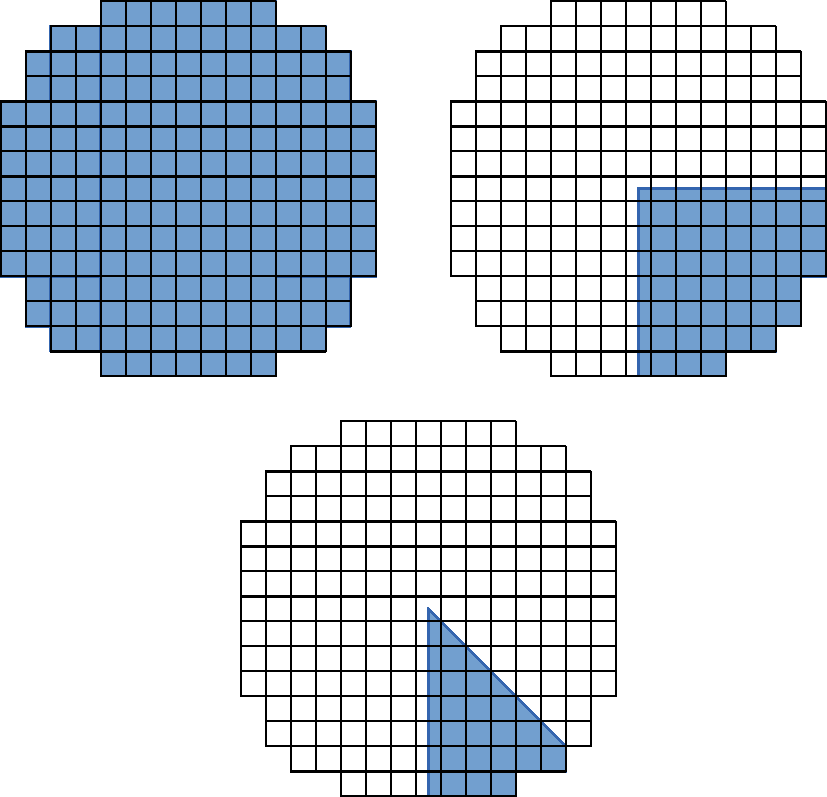
\includegraphics[width=5in]{figs/core_symmetry.pdf}
\end{center}
\caption{\label{fig:coresym} Full, quarter, and octant symmetry regions for a core map.}
\end{figure}

If there is an empty location in the map (e.g., if there is no detector or no control rod
in an assembly), then enter a dash (also known as a \textit{hyphen}) ``-'' for that location. The dash is significant and signifies an
empty location in the core map. (The dash indicates that something is missing, but it is still
a valid assembly location. The ``0'' in the {\it core\_shape} represents an invalid assembly location.)


\clearpage

The {\it assm\_map} shows where the assembly types are located within the core.
In the example below, there are three assembly types that will be defined in [ASSEMBLY] block(s).
\begin{Verbatim}[fontsize=\small]

  assm_map
                  A3 A3 A3 A3 A3 A3 A3
            A3 A3 A3 A1 A3 A1 A3 A1 A3 A3 A3
         A3 A3 A2 A1 A2 A1 A2 A1 A2 A1 A2 A3 A3
         A3 A2 A2 A2 A1 A2 A1 A2 A1 A2 A2 A2 A3
      A3 A3 A1 A2 A1 A2 A1 A2 A1 A2 A1 A2 A1 A3 A3
      A3 A1 A2 A1 A2 A1 A2 A1 A2 A1 A2 A1 A2 A1 A3
      A3 A3 A1 A2 A1 A2 A1 A2 A1 A2 A1 A2 A1 A3 A3
      A3 A1 A2 A1 A2 A1 A2 A1 A2 A1 A2 A1 A2 A1 A3
      A3 A3 A1 A2 A1 A2 A1 A2 A1 A2 A1 A2 A1 A3 A3
      A3 A1 A2 A1 A2 A1 A2 A1 A2 A1 A2 A1 A2 A1 A3
      A3 A3 A1 A2 A1 A2 A1 A2 A1 A2 A1 A2 A1 A3 A3
         A3 A2 A2 A2 A1 A2 A1 A2 A1 A2 A2 A2 A3
         A3 A3 A2 A1 A2 A1 A2 A1 A2 A1 A2 A3 A3
            A3 A3 A3 A1 A3 A1 A3 A1 A3 A3 A3
                  A3 A3 A3 A3 A3 A3 A3

\end{Verbatim}

The following map is equivalent to the previous map but demonstrates the use of input with octant symmetry.
Only values in the octant shown in Figure~\ref{fig:coresym} are entered in the map, and the parser automatically
unfolds the map to full symmetry.
\begin{Verbatim}[fontsize=\small]

  assm_map
     A1
     A2 A1
     A1 A2 A1
     A2 A1 A2 A1
     A1 A2 A1 A2 A2
     A2 A1 A2 A1 A2 A3
     A1 A3 A1 A3 A3 A3
     A3 A3 A3 A3         ! assembly map with octant symmetry

\end{Verbatim}

The {\it insert\_map} is used to show where assembly inserts are located within the core.
In the following quarter-symmetry example,
the inserts are burnable poison assemblies with different numbers of Pyrex rods.
The {\it insert\_map} can also be used to place geometry objects such as thimble plugs.
The geometry description of the inserts will be given in the [INSERT] block.
\begin{Verbatim}[fontsize=\small]

  insert_map
      -    BP20   -    BP20   -    BP20   -    BP12
     BP20   -    BP24   -    BP20   -    BP24   -
      -    BP24   -    BP20   -    BP16   -    BP8
     BP20   -    BP20   -    BP20   -    BP16   -
      -    BP20   -    BP20   -    BP24   -
     BP20   -    BP16   -    BP24  BP12   -
      -    BP24   -    BP16   -     -
     BP12   -    BP8    -

\end{Verbatim}
The {\it insert\_map} is optional if no inserts are present in the core.
A dash ``-'' is used to specify assembly locations without an insert.

The {\it det\_map} is used to show where detectors are located in the core. The geometry description
of the corresponding detector strings is given in the [DETECTOR] block. In this example,
there is only one detector type, denoted with a ``1''. Since the ``1'' occurs in a core map,
it is treated as a character string. This example uses a full-symmetry map.
\begin{Verbatim}[fontsize=\small]

  det_map
                 -  -  1  -  -  1  -
           1  -  -  1  -  1  -  -  -  -  -
        -  -  -  -  -  -  1  -  1  -  1  -  1
        1  1  -  -  -  -  1  -  -  -  -  -  -
     -  -  -  -  1  -  -  -  1  -  1  -  1  -  -
     1  -  1  -  -  1  -  1  -  -  -  -  -  1  -
     -  -  -  1  -  -  1  -  -  1  -  -  1  -  -
     1  -  1  -  1  -  1  -  -  1  -  1  1  1  -
     -  1  -  -  -  -  -  -  1  -  1  -  -  -  1
     -  -  -  -  1  -  1  -  -  -  -  1  -  -  -
     1  -  -  -  1  -  -  1  -  -  1  -  -  -  1
        -  -  -  -  1  -  -  1  -  -  1  -  -
        -  1  -  1  -  -  1  -  -  -  -  -  1
           1  -  -  -  1  -  -  1  -  1  -
                 1  -  -  1  -  -  -

\end{Verbatim}
The {\it det\_map} is optional if no detectors are present in the core.
A dash ``-'' is used to specify assembly locations without a detector.

% fix: Need to define what a control rod bank is

The control rod assemblies are described with two maps. The {\it crd\_map}
defines the control rod types and locations in the core.
The {\it crd\_bank} map assigns control rod locations to control rod banks.
The control rod maps are optional if no control rods are present in the core.
In the following example, there is only one control rod type, labeled ``1''.

\begin{Verbatim}[fontsize=\small]
  crd_map
                 -  -  -  -  -  -  -
           -  1  -  1  -  1  -  1  -  1  -
        -  -  -  1  -  1  -  1  -  1  -  -  -
        1  -  1  -  -  -  1  -  -  -  1  -  1
     -  -  1  -  1  -  -  -  -  -  1  -  1  -  -
     -  1  -  -  -  1  -  1  -  1  -  -  -  1  -
     -  -  1  -  -  -  -  -  -  -  -  -  1  -  -
     -  1  -  1  -  1  -  1  -  1  -  1  -  1  -
     -  -  1  -  -  -  -  -  -  -  -  -  1  -  -
     -  1  -  -  -  1  -  1  -  1  -  -  -  1  -
     -  -  1  -  1  -  -  -  -  -  1  -  1  -  -
        1  -  1  -  -  -  1  -  -  -  1  -  1
        -  -  -  1  -  1  -  1  -  1  -  -  -
           -  1  -  1  -  1  -  1  -  1  -
                 -  -  -  -  -  -  -
\end{Verbatim}
\vfill   % don't split map
\begin{Verbatim}[fontsize=\small]
  crd_bank
                 -  -  -  -  -  -  -
           - SA  -  B  -  C  -  B  - SA  -
        -  -  - SD  - SB  - SB  - SC  -  -  -
       SA  -  D  -  -  -  D  -  -  -  D  - SA
     -  - SC  -  A  -  -  -  -  -  A  - SD  -  -
     -  B  -  -  -  C  -  A  -  C  -  -  -  B  -
     -  - SB  -  -  -  -  -  -  -  -  - SB  -  -
     -  C  -  D  -  A  -  D  -  A  -  D  -  C  -
     -  - SB  -  -  -  -  -  -  -  -  - SB  -  -
     -  B  -  -  -  C  -  A  -  C  -  -  -  B  -
     -  - SD  -  A  -  -  -  -  -  A  - SC  -  -
       SA  -  D  -  -  -  D  -  -  -  D  - SA
        -  -  - SC  - SB  - SB  - SD  -  -  -
           - SA  -  B  -  C  -  B  - SA  -
                 -  -  -  -  -  -  -

\end{Verbatim}

%%%%%%%%%%%%%%%%%%%%%%%%%%%%%%%%%%%%%%%
\subsubsection{Core Baffle and Vessel}

The \textit{core baffle} or \textit{shroud} is a steel reflector that closely surrounds
the fuel assemblies in the core. The \textit{barrel} is a round steel structure that surrounds the baffle, and
the \textit{vessel} is the round outer pressure vessel. These structures are shown in
Figure~\ref{fig:corebaffle}.

\begin{figure}
\begin{center}
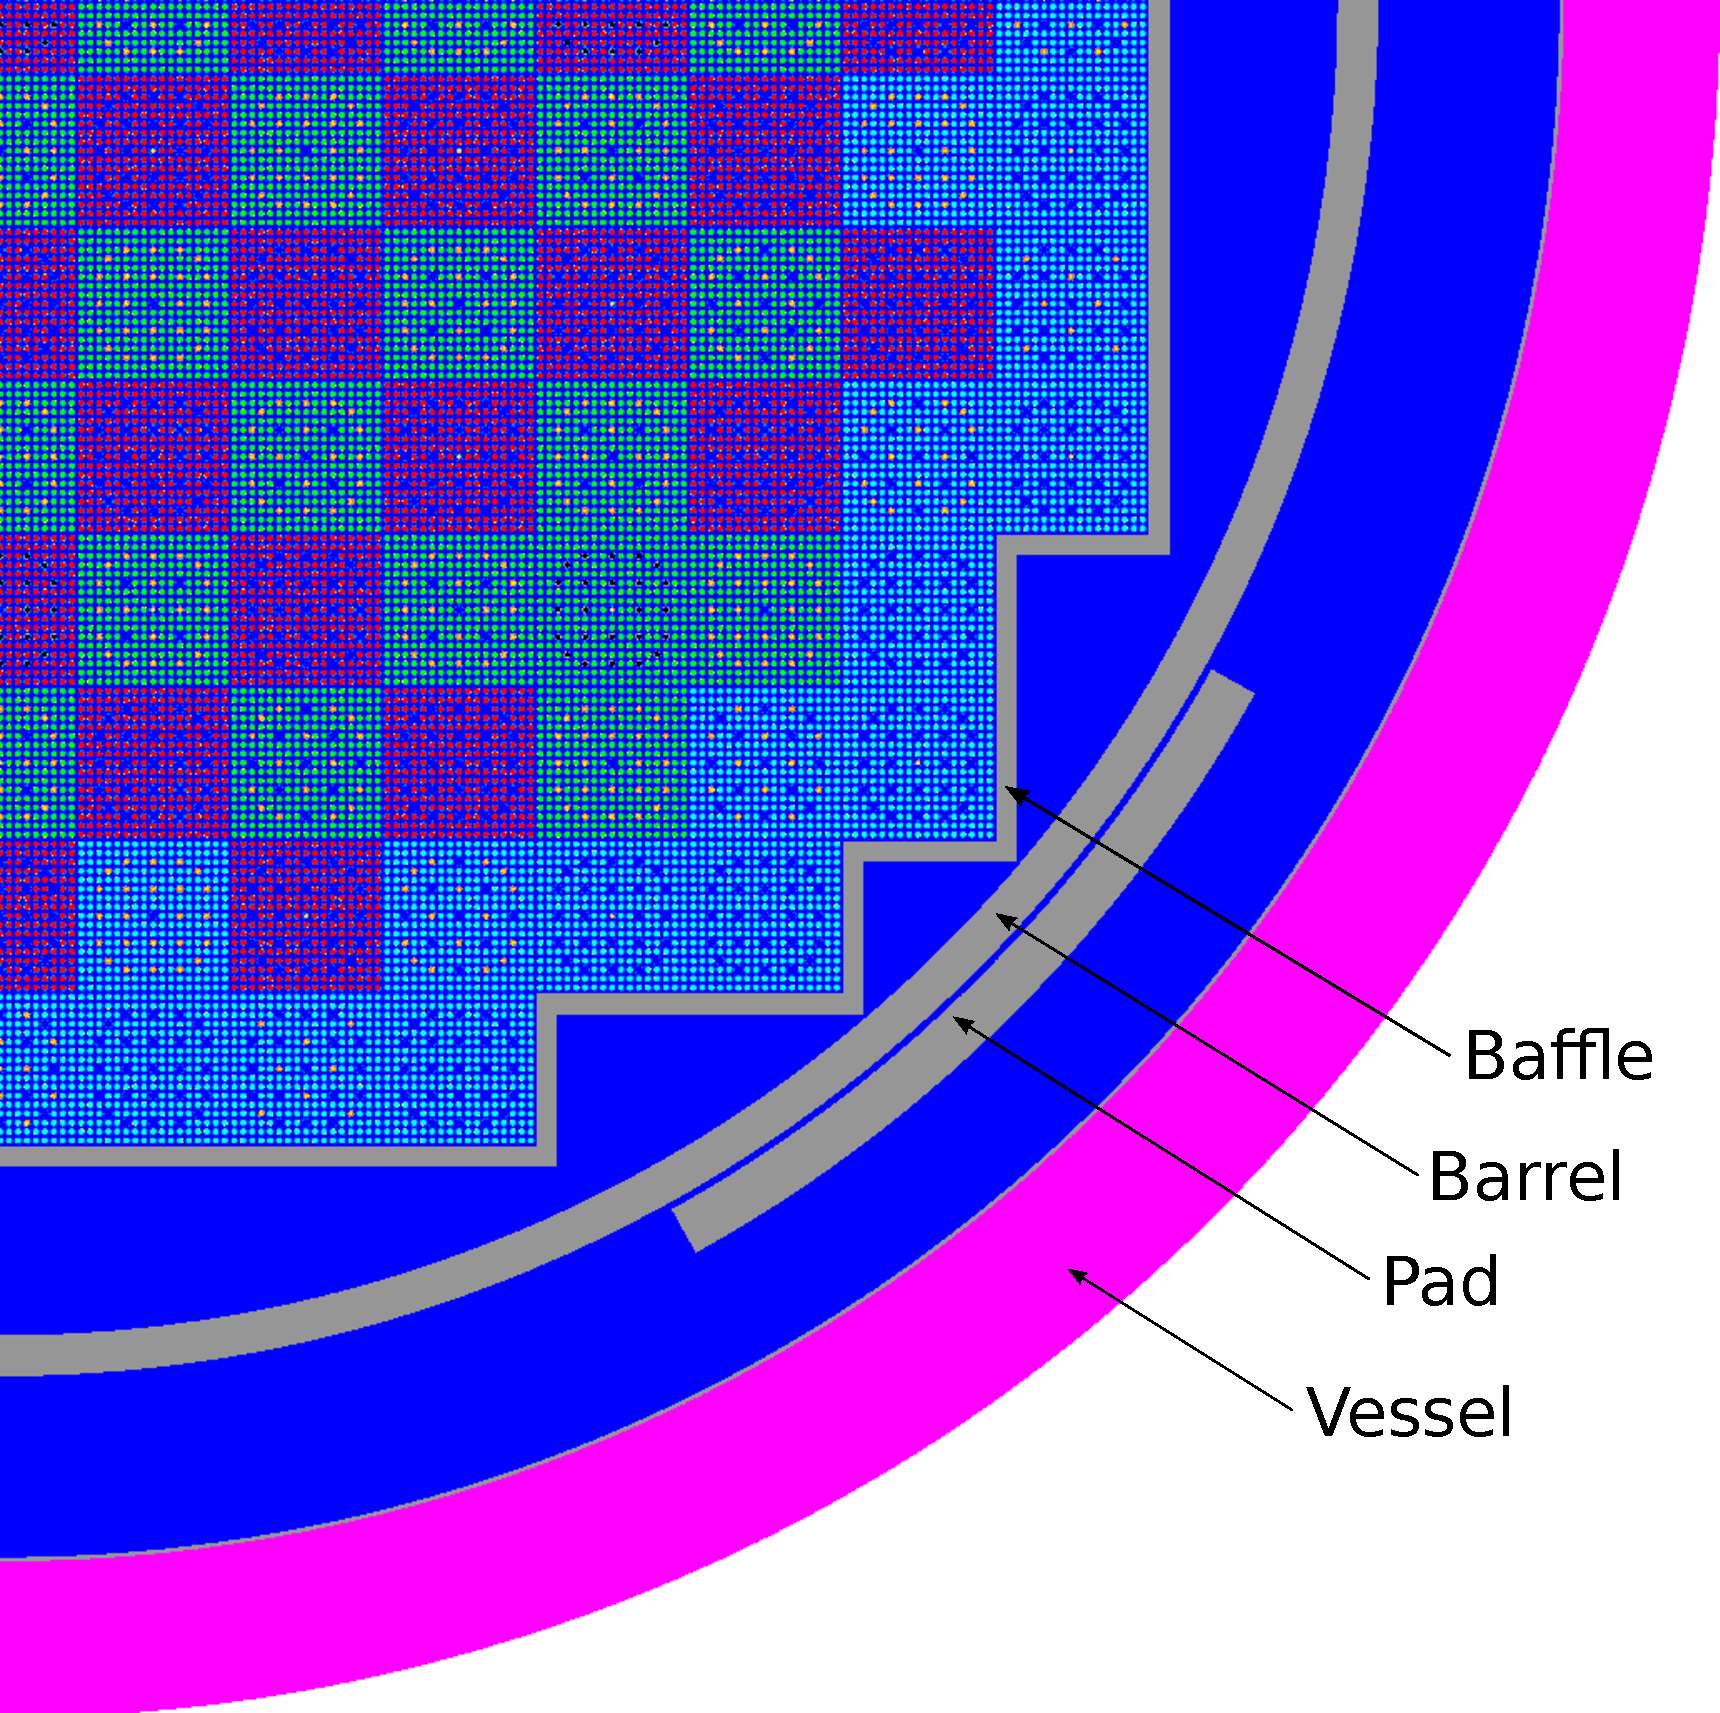
\includegraphics[width=5in]{figs/core_baffle.pdf}
\end{center}
\caption{\label{fig:corebaffle} Core baffle and vessel (image courtesy of Andrew Godfrey).}
\end{figure}

% fix: add figure showing exactly how the baffle gap is defined

The {\it baffle} is defined with a single material, the size of the gap between the
outer assembly and baffle, and the baffle thickness.
\begin{Verbatim}[fontsize=\small]

  baffle   SS304 0.19 1.26   ! material, gap (cm), and thickness (cm)

\end{Verbatim}

The barrel and vessel are defined with a {\it vessel} card. This card allows the
user to enter any arbitrary number of rings surrounding a core by specifying the
ring radii and the materials between the rings.

\begin{Verbatim}[fontsize=\small]

  vessel   mod 166.7 SS304 169.2 mod 175.0 SS304 176.0   ! materials and radii (cm)

\end{Verbatim}

There is currently no input defined to specify the neutron pad.

%%%%%%%%%%%%%%%%%%%%%%%%%%%%%%%%%%%%%%%
\subsubsection{Core Plates}

The core plates are large steel plates at the top and bottom of the core that have
various flow holes passing through them. All of the axial core heights are defined relative to the
top of the bottom core plate, and the total core {\it height} is defined as the distance
between the top of the bottom core plate and the bottom of the top core plate.

The core plates are modeled in the neutronics codes as smeared materials.
The upper and lower core plates are defined with a material composition, a thickness, and a
volume fraction of the structural material.
The remainder of the volume fraction is filled with coolant.

\begin{Verbatim}[fontsize=\small]

  lower_plate SS304  5.0  0.5   ! material, thickness (cm), volume fraction
  upper_plate SS304  7.6  0.5   ! material, thickness (cm), volume fraction
\end{Verbatim}

%%%%%%%%%%%%%%%%%%%%%%%%%%%%%%%%%%%%%%%
\subsubsection{Small Core Geometries}
\label{sec:smallcoregeom}

Even though the VERA input is designed for ``real'' core geometries, it can accommodate smaller
problems as well.
For example, to run a single-assembly calculation, the user would define the core size
as one assembly by one assembly, and all of the core maps would contain a single assembly.
\begin{Verbatim}[fontsize=\small]

  size 1                ! core composed of a single-assembly
  core_shape
     1

\end{Verbatim}

To model a single fuel rod, the user would define a core with one assembly and
an assembly with one rod in it.



%%%%%%%%%%%%%%%%%%%%%%%%%%%%%%%
%  Section: Assemblies
%*-------------------------------------------------------------------------*
%*                 Copyright 2013-2015 Core Physics, Inc.                  *
%*  Under terms of the contract to support CASL, there is a non-exclusive  *
%*  license for use of this work by or on behalf of the U.S. Government.   *
%*-------------------------------------------------------------------------*
%
% @version CVS $Id: assemblies.tex,v 1.23 2015/02/23 00:56:17 scott Exp $
%
%%%%%%%%%%%%%%%%%%%%%%%%%%%%%%%%%%%%%%%%%%%%%%%%%%%%%%%%%%%%%%%%
\subsection{Assembly Description}

The [ASSEMBLY] block contains the geometric description of a unique fuel assembly design (type).
Multiple [ASSEMBLY] blocks are permitted to describe different assembly designs in the core.

If there are multiple assembly designs that are geometrically identical (i.e., everything is the same except
the enrichments), then they can all be defined in a single [ASSEMBLY] block.
Each assembly type will have a unique {\it axial} card with possibly unique axial levels and lattice types.
Assemblies within a single reload typically have a design similar enough that they can share a single
[ASSEMBLY] block.

If assembly designs are not geometrically identical (e.g., if they are from different vendors or different generations), then
they need to be defined in separate [ASSEMBLY] blocks.
One advantage to having separate blocks for each assembly design is that each design can be
modeled (and archived) independently without the need to rely on global definitions.

A typical PWR assembly is shown in Figure~\ref{fig:assembly}. Refer to this figure in the following discussions.
\begin{figure}[hbt!]
\begin{center}
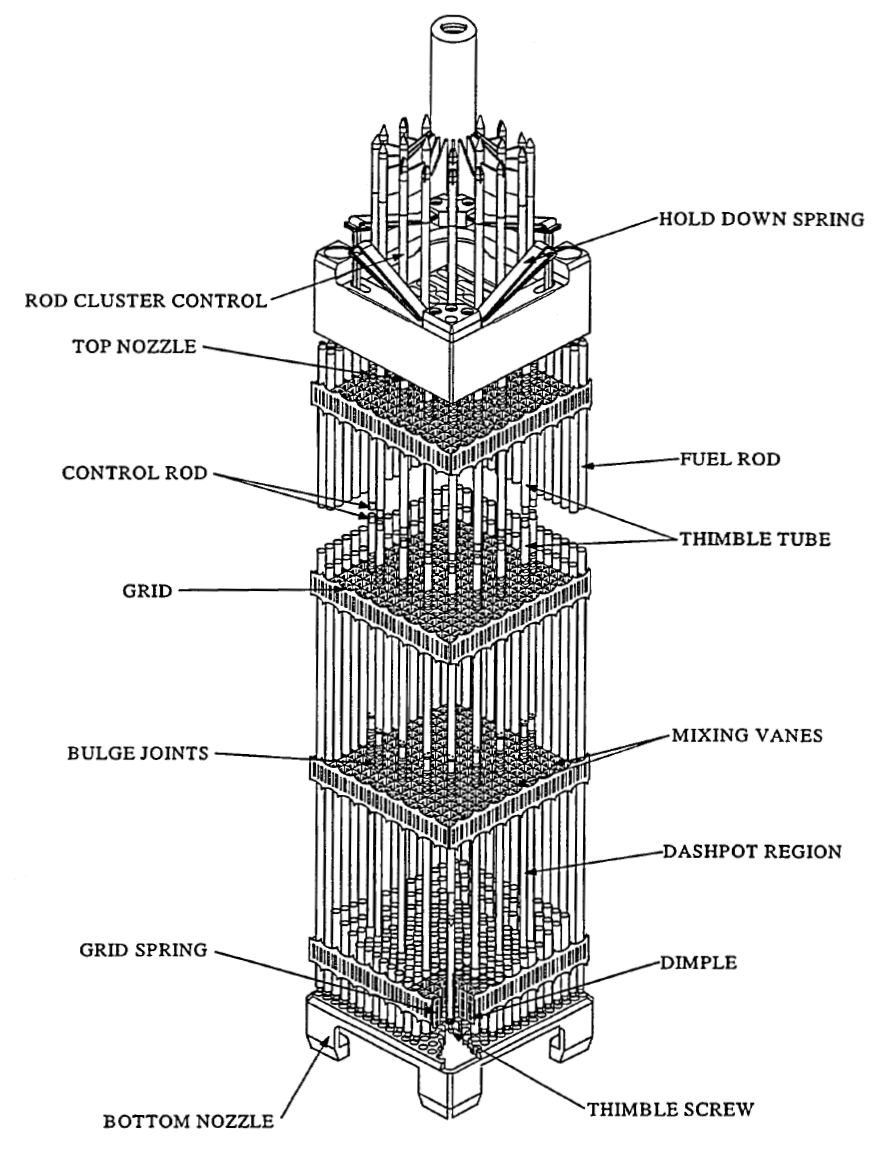
\includegraphics[scale=0.47]{figs/assembly.PNG}
\end{center}
\caption{\label{fig:assembly} PWR fuel assembly (Image courtesy of the US Nuclear Regulatory Commission).}
\end{figure}

A complete list of all the input cards in the [ASSEMBLY] block is located in Chapter~\ref{chap:cards}.

%%%%%%%%%%%%%%%%%%%%%%%%%%%
\subsubsection{Initial Data}

Each assembly block must contain a geometry description with the number of pins across the assembly and
the pin pitch.  An assembly block can also include an optional title card.
\begin{Verbatim}[fontsize=\small]

  title "Westinghouse 17x17"      ! assembly title
  npin 17                         ! number of pins across one side
  ppitch 1.260                    ! pin pitch (cm)

\end{Verbatim}

The number of pins {\it npin} must be the same for every assembly in a core.

The inter-assembly gap on each side of the assembly is calculated as $[apitch-npin*ppitch]/2$

For a boiling water reactor (BWR), a channel box may be specified with the following cards. See Section~\ref{sec:channel_box} for a complete
description of the channel box inputs.
\begin{Verbatim}[fontsize=\small]

  channel_box zirc 0.254 0.10         ! mat, corner thickness (cm), corner radius (cm)
  channel_box_segments 0.18 2.5 0.2   ! segment thickness (cm), segment length (cm),
                                      ! segment ramp (cm)

\end{Verbatim}

The fuel and structural materials are defined with the following cards.
See Chapter~\ref{chap:materials} for a complete description of the material inputs.
\begin{Verbatim}[fontsize=\small]

  fuel U31 10.257 95.0 / 3.1   ! mat, density (g/cc), Theoretical density (%)
                               !    / U-235 enrichment (%)
  mat inc   8.19               ! mat, density (g/cc)
  mat ss    8.0
  mat zirc4 6.56

\end{Verbatim}

%%%%%%%%%%%%%%%%%%%%%%%%%%%
\subsubsection{Cell Descriptions}

Cell cards are used to describe ``pincells.''  A pincell is defined as a configuration
of concentric cylinders (or rings) centered in a square region of coolant.
Cell configurations can be used to model fuel rods or guide tubes (GTs),
as shown in Figure~\ref{fig:pincell}.
\begin{figure}
\begin{center}
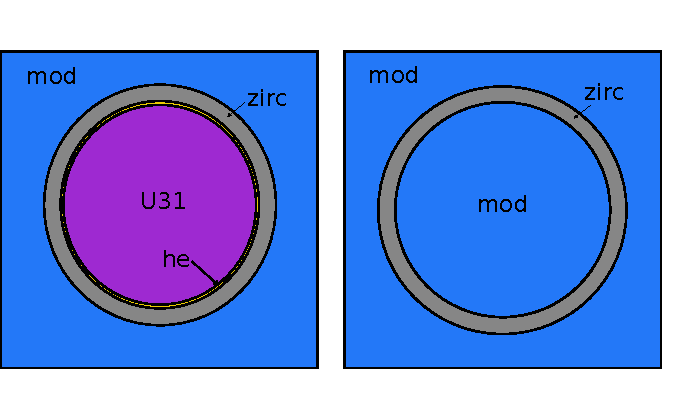
\includegraphics[width=4in]{figs/pincell1.pdf}
\end{center}
\caption{\label{fig:pincell} Pincell diagrams of a fuel rod and a guide tube.}
\end{figure}

The first parameter on the {\it cell} card is the cell ID.
This is followed by a list of radii for each ring in the cell, followed by a slash.
After the slash is a list of materials that comprise each ring.
The cell IDs are used in the rod maps described in the next section.

\begin{Verbatim}[fontsize=\small]

  cell 1     0.4096 0.418 0.475 / U31 he zirc4
  cell GT           0.561 0.602 / mod    zirc4      ! guide tube
  cell IT           0.561 0.602 / mod    zirc4      ! instrument tube
  cell 7            0.418 0.475 / mod    mod        ! empty location
  cell 8            0.418 0.475 /     he zirc4      ! plenum
  cell 9                  0.475 /        zirc4      ! pincap

\end{Verbatim}

In this example, in cell ``1,'' the material ``U31'' extends from radius 0 to 0.4096.
The material ``he'' extends from a radius 0.4096 to 0.418.
The materials ``U31''  and ``he'' are defined on {\it fuel} and {\it mat} cards, respectively.
(Refer to Chapter~\ref{chap:materials} for a complete description of material definitions.)

The outside of each cell is automatically filled with the special material ``mod,'' which
refers to the moderator (or coolant).
The composition of ``mod'' is calculated by the codes using the local thermal hydraulic (T/H) conditions and the
soluble boron concentration and cannot be specified by a user on a {\it mat} card.

In the example above, the GT and instrument tube (IT) descriptions
use the special moderator material ``mod'' to define the moderator material on both
the inside and outside of the tubes.

Large water rods that span more than one lattice cell can be specified by adding an optional keyword ``large4''
to the end of the {\it cell} card.
\begin{Verbatim}[fontsize=\small]

! large CE 16x16 water rod
  ppitch  1.28524
  cell WR 1.26 1.28 / mod zirc4 / large4

\end{Verbatim}

%%%%%%%%%%%%%%%%%%%%%%%%%%%
\subsubsection{Lattice Descriptions}

Once the cells are defined, they are placed into 2D ``lattices'' as shown below.
Like the core maps, lattice maps can be entered with either full-symmetry, quarter-symmetry,
or octant-symmetry. The maps below are octant-symmetric maps for 17$\times$17 assembly designs.
\vfill   % don't split map
\begin{Verbatim}[fontsize=\small]
  rodmap FUEL1
      IT
       1 1
       1 1 1
      GT 1 1 GT
       1 1 1  1 1
       1 1 1  1 1 GT
      GT 1 1 GT 1  1 1
       1 1 1  1 1  1 1 1
       1 1 1  1 1  1 1 1 1

  rodmap LGAP1
      IT
       7 7
       7 7 7
      GT 7 7 GT
       7 7 7  7 7
       7 7 7  7 7 GT
      GT 7 7 GT 7  7 7
       7 7 7  7 7  7 7 7
       7 7 7  7 7  7 7 7 7

  rodmap PLEN1
      IT
       8 8
       8 8 8
      GT 8 8 GT
       8 8 8  8 8
       8 8 8  8 8 GT
      GT 8 8 GT 8  8 8
       8 8 8  8 8  8 8 8
       8 8 8  8 8  8 8 8 8

  rodmap PCAP1
      IT
       9 9
       9 9 9
      GT 9 9 GT
       9 9 9  9 9
       9 9 9  9 9 GT
      GT 9 9 GT 9  9 9
       9 9 9  9 9  9 9 9
       9 9 9  9 9  9 9 9 9

\end{Verbatim}

Rod maps define each unique axial level in the assembly.
The first parameter is the lattice name (e.g., FUEL1 and PCAP1),
followed by a map of the {\it cell} IDs.

Each entry in a rod map must be a valid cell ID.

%%%%%%%%%%%%%%%%%%%%%%%%%%%
\subsubsection{Axial Descriptions}

After rod maps are defined for each axial level, the lattices are ``stacked'' into
an assembly using an {\it axial} card as shown below.

\begin{Verbatim}[fontsize=\small]
  axial A1    6.050
      LGAP1  10.281
      PCAP1  11.951
      FUEL1 377.711
      PLEN1 393.711
      PCAP1 395.381
      LGAP1 397.501

\end{Verbatim}

The {\it axial} card tells the code how to place the lattices axially.
The first parameter is the name of the assembly (A1), followed by a
list of elevations and lattice types.
For example, lattice ``FUEL1'' extends from 11.951 to 377.711 cm axially.

Multiple assembly types can be defined in a single [ASSEMBLY] block by using
multiple {\it axial} cards, each with a unique assembly ID.

All axial elevations are defined relative to the top of the lower core plate.

%%%%%%%%%%%%%%%%%%%%%%%%%%%
\subsubsection{Grid Spacer Descriptions}

Grid cards are used to define unique grid spacer types.
The following example defines two grid types, ``END'' and ``MID.''
\begin{Verbatim}[fontsize=\small]

  grid END inc    3.866 1017 / loss=0.9070  ! material, height(cm), mass (g), loss coef
  grid MID zirc4  3.810 875 / loss=0.9065

\end{Verbatim}

The grid types are placed axially with the {\it grid\_axial} card:
%\vfill   % don't split map
\begin{Verbatim}[fontsize=\small]

  grid_axial
      END  13.884
      MID  75.2
      MID 127.4
      MID 179.6
      MID 231.8
      MID 284.0
      MID 336.2
      END 388.2

\end{Verbatim}

The elevations are the midpoints of the spacer grid and are relative to the top of the lower core plate.

%%%%%%%%%%%%%%%%%%%%%%%%%%%
\subsubsection{Nozzle Descriptions}

The assembly nozzles are modeled in the neutronics codes as smeared materials. This approximation is
very good since the nozzles are not in the active fuel region and are mostly
composed of water, steel, and zirconium. The user only specifies a nozzle mass and a nozzle height.
The total volume of the nozzle region is calculated from the assembly pitch and nozzle height.
The volume of the nozzle is calculated from the nozzle mass and density.
The volume of the coolant is then calculated as the total volume minus the volume of the nozzle.
The coolant density is updated with the local T/H conditions.

% A typical PWR assembly nozzle is shown in Figure~\ref{fig:nozzle}.
% \begin{figure}
% \begin{center}
% 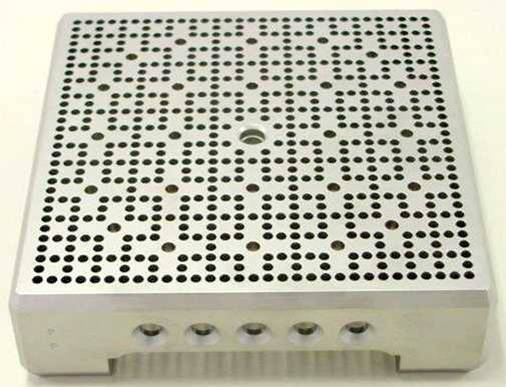
\includegraphics[width=4in]{figs/nozzle.jpg}
% \end{center}
% \caption{\label{fig:nozzle} PWR Assembly Lower Nozzle.}
% \end{figure}

\begin{Verbatim}[fontsize=\small]

  lower_nozzle  ss 6.05  6250.0  ! mat, height (cm), mass (g)
  upper_nozzle  ss 8.827 6250.0  ! mat, height (cm), mass (g)
\end{Verbatim}

Only a single material can be specified on a nozzle card.  To use
more than one material to define a nozzle, the user can define a custom material that
is a mixture of the materials and then use the custom material in the nozzle card.

Note that the {\it lower\_nozzle} height should match the bottom elevation on the {\it axial} card.
The {\it upper\_nozzle} height + the top elevation on the {\it axial} card must match the
core {\it height} in the [CORE] block.
The input parser does not currently perform a check to make sure the elevations are consistent.
Therefore, this check should be performed in each of the individual physics codes.

%%%%%%%%%%%%%%%%%%%%%%%%%%%%%%%%%%%%%%%%%%%%%%%%%%%%%%%%%%%
\subsection{Control Rod Assembly Description}

The [CONTROL] block contains the geometric description of a control assembly.

A control rod assembly is defined in a manner similar to that used to define a fuel assembly.
The user specifies cells, lattices, and axial descriptions of the control rod assembly.
The main difference between the control rod assembly and the fuel assembly is that
the control rod assembly describes what is inside the GTs, whereas the fuel assembly
defines the GTs themselves.

Control rod positions change during operation, so the geometric description of a control rod
should always be for a rod in the {\bf fully inserted} position.
In the example below, the bottom of the control rod in the fully inserted position is
at an axial location of 15.46 cm.

\begin{Verbatim}[fontsize=\small]

  title "B4C control rods with AIC tips"
  npin 17

  cell 1  0.382 0.386 0.484 / aic he ss      ! AIC cell
  cell 2  0.373 0.386 0.484 / b4c he ss      ! B4C cell

  rodmap  AIC
     -
     - -
     - - -
     1 - - 1
     - - - - -
     - - - - - 1
     1 - - 1 - - -
     - - - - - - - -
     - - - - - - - - -

  rodmap  B4C
     -
     - -
     - - -
     2 - - 2
     - - - - -
     - - - - - 2
     2 - - 2 - - -
     - - - - - - - -
     - - - - - - - - -

  axial CR1 15.46 AIC  376.44 B4C  394.3

\end{Verbatim}

The name of the control rod ``CR1'' refers to the control rod type in the
{\it crd\_map} in the [CORE] block.

Control rod positions are assigned to a control rod bank with the {\it crd\_bank} map
in the [CORE] block, and then the banks are positioned with the
{\it rodbank} card in the [STATE] block.

Note that the locations of the control rod fingers must match the GT locations in the
corresponding [ASSEMBLY] block descriptions.  Furthermore, the outer radii of the control
rod fingers must be smaller than the inner radii of the GTs.
The input parser does not currently perform a check to make sure the control rod finger
descriptions are consistent with the GT descriptions.
This check should be performed in each of the individual physics codes.

The user can define materials in the [CONTROL] block.  These materials only have scope in
this block and are not accessible by other blocks. See Chapter~\ref{chap:materials} for details.

A complete list of all the input cards in the [CONTROL] block is provided in Chapter~\ref{chap:cards}.

%%%%%%%%%%%%%%%%%%%%%%%%%%%
\subsubsection{Control Rod Stroke}
\label{sec:stroke}

The difference between control rod descriptions and assembly descriptions is that
the control rods move during operation. This movement is defined with a {\it stroke} card.

The first value on the {\it stroke} card is the total length of the control rod travel (stroke)
from fully inserted to fully withdrawn.

The second value on the {\it stroke} card is the number of steps in the fully withdrawn position.
Step 0 is the fully inserted position. The number of steps in the fully withdrawn position
is specified by the user, but 228 steps is often the number used for typical Westinghouse PWRs.

\begin{Verbatim}[fontsize=\small]

  stroke  360.0 228      ! stroke (cm), number of steps fully withdrawn

\end{Verbatim}

To position the control rods in percent withdrawn (\%), the number of steps should be set to 100, and
each step will signify 1\% withdrawn.

The geometry description in the input is for a control rod in the fully inserted position (step 0).

\subsubsection{Control Rod Position Example}

From the {\it axial} card shown above, the bottom of the AIC at the fully inserted position is 15.46 cm.
From the {\it stroke} card, the total stroke is 360.0 cm, and the number of steps in the fully withdrawn
position is 228 steps.
Therefore, the bottom elevation of the AIC lattice at step \textit{N} will be
\begin{equation}
   E(N) = 15.46 + \frac{360.0 \cdot N}{228}
\end{equation}

Using this formula, the bottom elevation of the AIC lattice at the following step positions is as follows:
\begin{itemize}   % itemize = bullet list
 \item step 228 (fully withdrawn) = 15.46 + 360.0 * 228 / 228 = 375.46 cm
 \item step 100 = 15.46 + 360.0 * 100 / 228 = 173.35 cm
 \item step 0 (fully inserted) = 15.46 + 360.0 * 0 / 228 = 15.46 cm
\end{itemize}

The steps withdrawn can be specified as real numbers and fractions of a step.

%%%%%%%%%%%%%%%%%%%%%%%%%%%%%%%%%%%%%%
\subsection{Insert Description}
An assembly insert is defined in the same way as a fuel assembly or control rod assembly.
The user defines the insert using cells, lattices, and axial descriptions.

The fuel assembly description should contain the GT descriptions, and the insert description
defines what is inserted into the GTs. Assembly inserts can be inserted and withdrawn
during a core shuffle (by specifying an {\it insert\_map} card in the [CORE] block),
but they cannot be moved during a cycle depletion.

The insert and control rod descriptions are very similar, with the only difference being that the
insert cannot change position axially during a cycle depletion, and a control rod moves axially
during operations.

The following example shows a definition of a Pyrex insert.

\begin{Verbatim}[fontsize=\small]

[INSERT]
    title "Pyrex"
    npin 17
    mat pyrx1 2.25 pyrex-vera
    cell 1  0.214 0.231 0.241 0.427 0.437 0.484 / he ss he pyrx1 he ss
    rodmap  PY24
       -
       - -
       - - -
       1 - - 1
       - - - - -
       - - - - - 1
       1 - - 1 - - -
       - - - - - - - -
       - - - - - - - - -

    axial INS24  15.76 PY24 376.441

\end{Verbatim}

The name of the insert ``INS24'' refers to an insert type defined in the
{\it insert\_map} in the [CORE] block.

The locations of the insert fingers must match the GT locations in the
corresponding [ASSEMBLY] block descriptions.  In addition, the outer radii of the insert
fingers must be smaller than the inner radii of the GTs.
The input parser does not currently perform a check to make sure the insert finger
descriptions are consistent with the GT descriptions.
This check should be performed in each physics code.

As with [ASSEMBLY] blocks, multiple insert types can be defined in a single [INSERT]
block by using multiple {\it axial} cards, each with a unique insert ID.

A complete list of all the input cards in the [INSERT] block is provided in Chapter~\ref{chap:cards}.

%%%%%%%%%%%%%%%%%%%%%%%%%%%%%%%%%%%%%%
\subsection{Detector Description}
A detector string is defined in the same way that a fuel assembly or insert assembly is defined.
The user defines cells, lattices, and axial descriptions for the detector string.

The insert and detector descriptions are very similar, with the difference being that
detectors have special properties used to calculate instrumentation signals.
\vfill   % don't split map
\begin{Verbatim}[fontsize=\small]
  [DETECTOR]
    title "Incore instrument thimble"
    npin 17

    mat he 0.0001786
    mat ss 8.0

    cell 1  0.258 0.382 / he ss

    rodmap  LAT
       1
       - -
       - - -
       - - - -
       - - - - -
       - - - - - -
       - - - - - - -
       - - - - - - - -
       - - - - - - - - -

    axial D1  0.0 LAT 406.337

\end{Verbatim}

The name of the detector ``D1'' refers to a detector type defined in the
{\it det\_map} in the [CORE] block.

A complete list of all the input cards in the [DETECTOR] block is located in Chapter~\ref{chap:cards}.

%%%%%%%%%%%%%%%%%%%%%%%%%%%%%%%%%%%%%%
\subsection{Channel Box}
\label{sec:channel_box}

The channel box that surrounds a BWR assembly may be modeled with the {\it channel\_box} and
{\it channel\_box\_segments} cards. The {\it channel\_box} card allows the representation of a normal box
with a nominal thickness and rounded corners. When paired with the {\it channel\_box\_segments} card,
a general explicit geometry of thick-thin designs may be modeled.

The card inputs are shown in Figure~\ref{fig:cbcard}.

\begin{figure}[h]
\begin{center}
  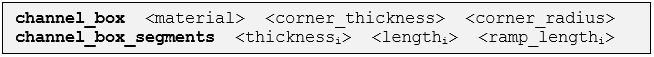
\includegraphics[width=5in]{figs/chanboxcard.jpg}
\end{center}
\caption{\label{fig:cbcard} Description of the channel box cards.}
\end{figure}

All of the dimensional quantities are in units of centimeters. The segment length and segment
ramp are deltas in length. The segment ramp should be entered as the horizontal distance
and not the slope. The definitions of the inputs are illustrated in Figure~\ref{fig:cbinputs}.
\begin{figure}[h]
\begin{center}
  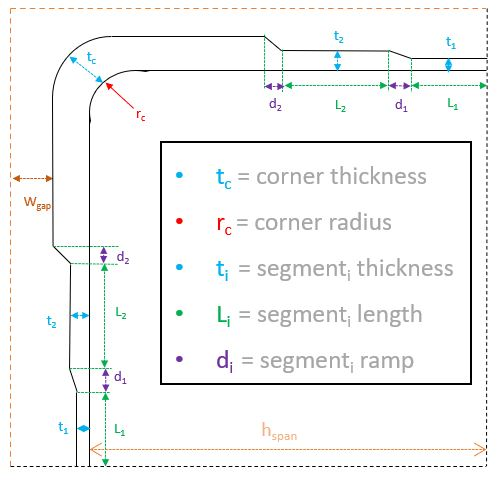
\includegraphics[width=3in]{figs/chanboxinputs.jpg}
\end{center}
\caption{\label{fig:cbinputs} Demonstration of the channel box cards.}
\end{figure}

The first channel box segment is entered at the halfspan of the box.
Each additional segment is entered in the direction of the corner.
It is assumed that the channels are symmetric about the corner and that all corners are alike.
The thick corner length is internally calculated from the given channel segments.

For both the normal and thick-thin channel box designs, the wide and narrow gaps should be
entered relative to the corner thickness. For the normal box, this is equivalent to the nominal
channel thickness.

Sample inputs are provided in Figure~\ref{fig:cbexample}.
\begin{figure}[h]
\begin{center}
  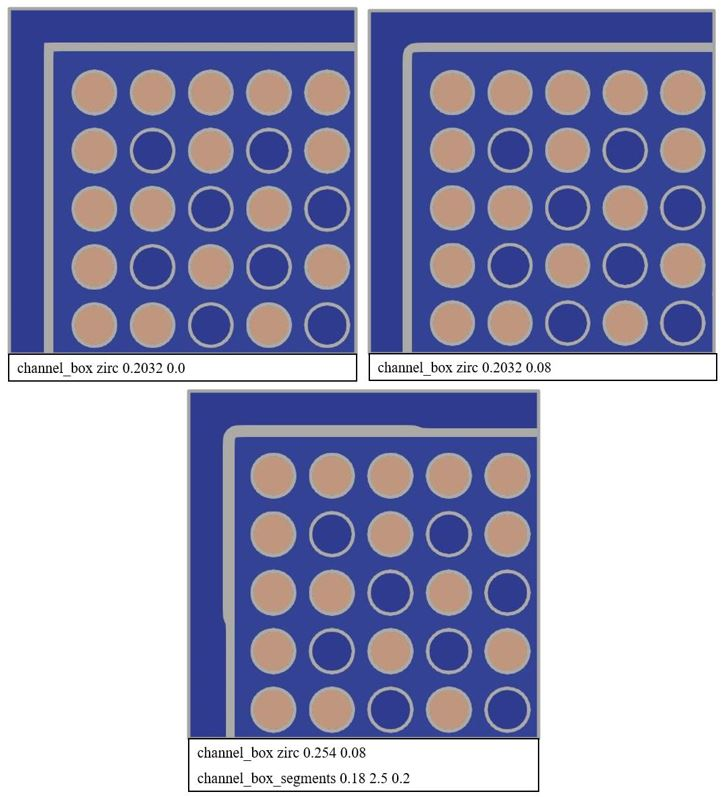
\includegraphics[width=4.5in]{figs/channelbox.jpg}
\end{center}
\caption{\label{fig:cbexample} Sample inputs for the channel box cards.}
\end{figure}

A complete list of the channel box cards is located in Chapter~\ref{chap:cards}.



%%%%%%%%%%%%%%%%%%%%%%%%%%%%%%%
%  Section: State
%*-------------------------------------------------------------------------*
%*                 Copyright 2013-2015 Core Physics, Inc.                  *
%*  Under terms of the contract to support CASL, there is a non-exclusive  *
%*  license for use of this work by or on behalf of the U.S. Government.   *
%*-------------------------------------------------------------------------*
%
% @version CVS $Id: state.tex,v 1.5 2015/02/17 03:26:30 Scott Exp $
%
%%%%%%%%%%%%%%%%%%%%%%%%%%%%%%%%%%%%%%%%%%%%%%%%%%%%%%%%%%%%%%%%
\subsection{State Description}

The [STATE] block defines the state of the core
(power, flow, pressure, inlet temperature, rod positions, boron concentration, etc.)
at a particular point in time.
These values will typically change during a cycle depletion.

An example showing the most common input cards in the [STATE] block is shown below.
A complete listing of all the input cards in the [STATE] block is located in Chapter~\ref{chap:cards}.

\begin{Verbatim}[fontsize=\small]
  [STATE]
    power   98.0       ! % of rated power - rated values defined in [CORE] block
    flow   100.0       ! % of rated flow
    pressure 2250.0    ! psia
    tinlet 557.33 F    !
    feedback on        ! turn on T/H feedback

    boron   1285       ! initial boron ppmB
    search  boron      ! turn on boron search

    sym qtr            ! run problem in qtr-symmetry

    rodbank SA 228
            SB 228
            SC 228
            SD 228
             A 228
             B 228
             C 228
             D 167
\end{Verbatim}

The {\it sym} card tells the code to run the calculation in full-core or
qtr-core symmetry. If the calculation is run in qtr-core symmetry, the symmetry is either
set to qtr-core rotational or qtr-core mirror by the {\it bc\_sym} card in the [CORE] block.

The {\it rodbank} card is used to position the control rods. The {\it rodbank} input includes pairs of bank names
and bank positions.  The bank names correspond to the {\it crd\_map} in the [CORE] block.
The positions indicate the position of the control rod bank in steps.
Step 0 is fully inserted.
The number of steps for a rod to be completely withdrawn is set by the {\it stroke} card in
the [CONTROL] block (see Section~\ref{sec:stroke}). For Westinghouse PWR's, a typical value of fully-withdrawn is 228 steps.

%%%%%%%%%%%%%%%%%%%%%%%%%%%%%%%
\subsection{Edits Description}

The [EDITS] block is used to control the output edits.

One of the edits produced by the core simulator is the rod power.   The user has
the ability to specify the axial levels that the power is averaged over with
the {\it axial\_edit\_bounds} card.
The user may choose to average power over uniform axial intervals (like most nodal codes),
or to specify the edit intervals manually.

(Note: the edit options are under development and more options will be added in the future.)

A complete listing of all the input cards in the [EDITS] block is located in Chapter~\ref{chap:cards}.

\subsubsection{CTF Nodalization}

The {\it axial\_edit\_bounds} card is also used to set the axial nodalization when coupling
the neutronics physics code to the CTF subchannel code.

When running CTF, there is a restriction that the grid boundaries must be explicitly
included in the {\it axial\_edit\_bounds}. This can get a little complicated for the user.
In the VERA input, spacer grids are defined in the [ASSEMBLY] block by specifying the
grid heights on the {\it grid} card and the elevations of the grid midpoints
on the {\it grid\_axial} card.
From the grid heights and midpoints, the elevations at the top and bottom of the spacer grid
can be calculated, and then the top and bottom elevations must be included
in the {\it axial\_edit\_bounds}.

For example, if a grid is defined with a centerline at 75.0 and a height of 2.5, then the
{\it axial\_edit\_bounds} must include the points $75.0 \pm 1.25 = 73.75$ and $76.25$.

\begin{Verbatim}[fontsize=\small]
   [ASSEMBLY]
    grid GRID1 inc 1000 2.5    ! grid name, material, mass (g), and height (cm)
    grid_axial                 ! locations of grid midpoints (cm)
        GRID1 75.0

   [EDITS]
    axial_edit_bounds
       ...
       73.75           ! this array must include top and bottom grid boundaries
       76.25
       ...
\end{Verbatim}

The reason for this restriction is because the power is calculated on the {\it axial\_edit\_bounds},
so it is natural to use the same power distribution to couple to the CTF model as well.
The grids must be explicitly included in the CTF boundaries so the loss coefficients are calculated correctly.

In the future, this restriction may be lifted and an additional edit bounds array may
be added explicitly for CTF calculations.


%%%%%%%%%%%%%%%%%%%%%%%%%%%%%%%
\subsection{Coupling Description}

The [COUPLING] block defines the relaxation parameters and convergence criteria to be
used when coupling different physics codes.  These values are used to determine
convergence {\it between} physics codes.  Convergence criteria {\it within} a physics
code is controlled by the code-specific block.

Refer to Chapter~\ref{chap:cards} for a complete listing of all the cards in the [COUPLING] block.

No code-specific information is included in the [COUPLING] block.  All code-specific information
is contained in the code-specific blocks.  The [COUPLING] block is only used to define
generic coupling parameters.

As an example, consider the following multi-physics code coupling:
\begin{enumerate}
  \item  Run T/H calculation
  \item  Run neutronics calculation
  \item  Check eigenvalue convergence \label{stepepsk}
  \item  Check power convergence \label{stepepsp}
  \item  Relax/dampen the power shape
  \item  If not converged, go to step 1.
\end{enumerate}
The eigenvalue convergence in step~\ref{stepepsk} uses the card {\it epsk} to check
the change in eigenvalue between coupled iterations.
There are additional eigenvalue convergence criteria {\it within} the neutronics
code, but the internal parameters are specified in the individual code blocks.

The power convergence in step~\ref{stepepsp} uses the card {\it epsp} to check
the change in power between coupled iterations.

Additional convergence checks are made on the peak fuel temperature, maximum change in density,
and change in boron concentration (if applicable).

The example shown above uses a Picard iteration to converge.  Picard iterations usually
need to apply a relaxation factor (also called a damping factor or under-relaxation factor) to
one or more of the calculated quantities to converge.
The relaxation factors are applied in the following manner:
\begin{equation}
  x = \omega \, x^{\mbox{new}} + (1 - \omega) x^{\mbox{old}}
\end{equation}
where $x$ is the calculated parameter and $\omega$ is the relaxation factor.
A relaxation factor of 1.0 signifies no relaxation is performed.
A relaxation factor $< 1.0$ signifies under-relaxation.

Relaxation factors can be specified for the point-wise power, point-wise temperature, and/or point-wise density.
The relaxation is applied to the transferred quantities sent between physics codes.  The state variables
within each physics code are not changed.

An example [COUPLING] input block is shown below.

\begin{Verbatim}[fontsize=\small]
   [COUPLING]
     epsk        5.0  ! eigenvalue convergence (pcm)
     eps_temp    1.0  ! temperature convergence (deg C)
     eps_boron   0.1  ! boron convergence (ppm)
     rlx_power   0.5  ! power relaxation factor
     rlx_tfuel   1.0  ! fuel temperature relaxation factor
     rlx_den     1.0  ! density relaxation factor
     maxiter     20   ! maximum number of coupled iterations
\end{Verbatim}

A complete listing of all the input cards in the [COUPLING] block is located in Chapter~\ref{chap:cards}.



%%%%%%%%%%%%%%%%%%%%%%%%%%%%%%%%%%%%%%%%%
%  Chapter: Materials
%*-------------------------------------------------------------------------*
%*                 Copyright 2013-2015 Core Physics, Inc.                  *
%*  Under terms of the contract to support CASL, there is a non-exclusive  *
%*  license for use of this work by or on behalf of the U.S. Government.   *
%*-------------------------------------------------------------------------*
%
% @version CVS $Id: materials.tex,v 1.22 2015/02/23 00:56:17 scott Exp $
%
%%%%%%%%%%%%%%%%%%%%%%%%%%%%%%%%%%%%%%%%%
\section{Materials}  \label{chap:materials}

This chapter contains a description of the material input.  There are two types of materials
in the input file -- structural materials (input with a {\it mat} card) and fuel materials
(input with a {\it fuel} card).

Structural materials can be defined in either the [CORE] block, or in the
geometry object blocks [ASSEMBLY], [INSERT], [CONTROL], and [DETECTOR].
If the materials are defined in the [CORE] block, they have global scope.
If the materials are defined in the geometry object blocks, they only have
scope in the block they are defined.
The reason for this is to maintain the modularity of the geometry objects.

Fuel materials can only be defined in [ASSEMBLY] blocks.

Materials are used in many different input cards.  They are used to define
cells, nozzles, core plates, baffles, grids, reflectors, etc.  Every material
used in the input must be defined with either a {\it mat} card or a {\it fuel} card
(see notes on the material ``mod'' below).

%%%%%%%%%%%%%%%%%%%%%%%%%%%%%%%%
\subsection{Structural Materials}

Structural materials are not fuel and do not deplete.  Structural
materials are defined with the following input card:

{\bf mat} {\it user-mat} {\it density} ({\it library-name$_i$}, {\it frac$_i$}, i=1, I)

where:
\begin{itemize}
\item {\it user-mat} is a user-defined material name.  The name is case sensitive.  {\it user-mat} is used to
define material names in other input cards such as {\it cell}, {\it grid}, {\it nozzle}, etc. (No default)
\item {\it density} is the material density in g/cc (No default)
\item {\it library-name} is a corresponding library name(s) for the user material.  The library name
must be defined in the cross section library. (Default = {\it user-mat}).  Multiple library materials
can be mixed to form a single user material.
\item {\it frac}  is the fraction of the library material in the user material. (Default=1.0 if there is only one library material in the user material).
\end{itemize}

There are two special user materials,  ``mod'' and ``vacuum''.
The user can use these materials in cell definitions, but the code will automatically
determine the composition of these materials  based on T/H feedback and soluble boron concentrations.
The user is not allowed to define a user material named ``mod'' or ``vacuum'' on a {\it mat} card.

Some example material cards are shown below.
\begin{Verbatim}[fontsize=\small]
  mat zirc4 6.56                   ! library-name defaults to user-name
  mat zirx  6.56 zirc4 1.0         ! user-name does not equal to library-name
  mat B10   12.0 boron 1.0
  mat XYZ   6.0  zirc4 0.8 ss 0.2  ! define new mixture of 80% zirc4 and 20% ss
  mat ABCD  8.0  zirc4 0.8 ss 0.15 b4c 0.05
  mat waba  3.65 b-10  1.36210E-02 ! creates material from isotopes in the XS-library
                 b-11  6.02818E-02
                 c-00  2.05259E-02
                 o-16  4.26297E-01
                 al-27 4.79274E-01
\end{Verbatim}

%% Fixed bug Andrew found below ~Feb 2014, atomic and weight were switched
All of the material fractions must sum to either +1.0 or -1.0.
If positive fractions are used, the fractions refer to weight fractions.
If negative fractions are used, the fractions refer to atomic fractions.

%%%%%%%%%%%%%%%%%%%%%%
\subsubsection{Search Order}

Structural materials can be defined in either the [CORE] block or one of the
geometry object blocks.  When a material is referred to in a block, it will look
for the material definition in the following order:
\begin{enumerate}  % enumerate = numbered list
 \item The code will first look for the material name in the local block ([ASSEMBLY], [INSERT], [CONTROL], or [DETECTOR])
 \item If the material is not found in the local block, it will look in the [CORE] block
\end{enumerate}

If materials are defined in the [CORE] block, they have global scope over the entire input.
If materials are defined in other blocks, they only have scope over the local block.  This means
that two geometry object blocks can use different material definitions with the same name.
One example of this is that two assemblies can be defined with the material ``zirc'', but
the ``zirc'' can have different compositions in each of the assemblies.

%%%%%%%%%%%%%%%%%%%%%%%%%%
\subsection{Default Materials}

There are many default files available to the users.  The default materials and their compositions
are defined on the initialization file CORE.ini.
A list of default materials is given in Table~\ref{table:mat}.
\begin{table}
\centering
\caption{Default Material List}
\label{table:mat}
\begin{tabular}{|c|c|l|}
\hline
  material  & density (g/cc)  & Notes \\
\hline
   air    &  1.189E-03  &        \\
   aic    &     10.2   &  silver-indium-cadmium      \\
   al2o3  &     3.96   &        \\
   b2o3   &     2.55   &        \\
   b4c    &   1.7597   &  boron carbide      \\
   boron  &     2.37   &        \\
   cs     &     7.85   &  carbon steel      \\
   gad    &     7.407  &        \\
   gap    & 0.17860E-03 &        \\
   he     & 0.17860E-03 &        \\
   inc    &    8.19    &  inconel      \\
   pyrex  &    2.34249 &        \\
   pyrex-vera& 2.24419 &        \\
   sio2     &   2.18   &        \\
   ss       &   8.0    &  stainless steel      \\
   tungsten &  19.3    &        \\
   water    &   0.743  &        \\
   waba     &   3.65   &        \\
   zirc2    &   6.56   &  Zircaloy-2      \\
   zirc4    &   6.56   &  Zircaloy-4      \\
   clad     &  6.56    &        \\
   zirc4-xhf&  6.55934 &  Zircaloy-4 with no Hf   \\
   zr       &  6.506   &  natural zirconium    \\
\hline
\end{tabular}
\end{table}

%%%%%%%%%%%%%%%%%%%%%%%%
\subsection{Fuel Materials}

Fuel materials are defined with {\it fuel} cards.
Fuel materials are heavy metal oxides which are usually UO$_2$ with different U-235 enrichments.
Fuel materials may also include MOX fuel, which consists of mixtures of uranium, plutonium and other actinides.
Fuel materials may also contain integral burnable absorbers, such as gadolinia.
Fuel materials are different from structural materials in that they deplete and have
additional properties as described below.

Fuel can only be defined in [ASSEMBLY] blocks, and fuel materials can only be referenced by {\it cell} cards
in the [ASSEMBLY] block they are defined in.

Fuel materials are defined with the following input card:

{\bf fuel} {\it user-mat} {\it density} {\it thden} / {\it U-235\_enrichment}
    \{{\it HM\_material$_i$}={\it HM\_enrichment$_i$}, i=1, N\}  \\
   \{ / {\it gad\_material}={\it gad\_fraction} \}

Where:
\begin{itemize}   % itemize = bullet list
  \item {\it user-mat} is a user-defined fuel name. It is case sensitive. (No default)
  \item {\it density} is the fuel material density in g/cc (No default).
     The density is used to calculate number densities.
  \item {\it thden} is the percent of theoretical density in the pellet (\%) (No default).
   The theoretical density is only used to look up material properties in the fuel performance,
   it is not used to calculate number densities.  There is no ``double counting'' between
   {\it density} and {\it thden}.
  \item {\it U-235\_enrichment} is the U-235 enrichment in the fuel in weight \%  (No default).
  \begin{itemize}   % itemize = bullet list
    \item If U-234 and U-236 are not specified, they will automatically be added to the
       fuel by a pre-determined function (see below)
    \item If the sum of the heavy metal (HM) enrichments does not equal 100\%, the remainder of the
        HM composition will be assigned to U-238.
  \end{itemize}
  \item {\it HM\_material$_i$} is the material name for HM isotope $i$ (Pu-239, Pu-241, etc.) (optional)
    The names of the HM materials must be valid library-names.
  \item {\it HM\_enrichment$_i$} is the enrichment of HM isotope $i$ in weight \% (optional)
  \item {\it gad\_material} is the material name for gadolina (or other integral burnable absorber material) (optional).
        The gad material is usually a mixture defined on a separate {\it mat} card.
  \item {\it gad\_fraction} is the weight percent of the gad material relative to the total fuel mass (optional)
\end{itemize}

Oxygen should not be included on the {\it fuel} card.  The correct amount of oxygen will automatically
be added to the HM to create an oxide (either UO$_2$  or (HM)O$_2$).

The {\it density} is the ``stack density'' or ``smeared density'' and should include the volume
of the pellet dishing and chamfers.
It is calculated as the total mass of the fuel pellets divided by the total volume of the fuel
\begin{equation}
  \mbox{stack density} = \frac{ (\mbox{fuel mass})} { \pi (\mbox{pellet radius})^2 \, (\mbox{fuel height}) }
\end{equation}

The {\it thden} refers to the actual theoretical density of the pellet.  This quantity may be
used in fuel performance codes to evaluate material properties.

If U-234 or U-236 enrichments are not included in the fuel definition, they are automatically
added to the fuel with the following formulas:
\begin{equation}
   W_{234} = 0.0089 \cdot W_{235}
\end{equation}
\begin{equation}
  W_{236} = 0.0046 \cdot W_{235}
\end{equation}
Where $W_{23x}$ is the enrichment of each of the uranium isotopes
in percent\footnote{Earlier versions of the code used a different formula for the default U-234 concentration.}.

If a user specifically does NOT want U-234 or U-236, they should specify a U-234
and/or U-236 enrichment of zero.

Examples of typical {\it fuel} cards are shown below.  The user
only has to specify the U-235 enrichment and the code will automatically add
U-234, U-236, U-238, and oxygen to the fuel.
\begin{Verbatim}[fontsize=\small]
  fuel U21 10.4 95.2 / 2.1        ! 2.1% enriched UO2 fuel, no gad
  fuel UO2-35 10.297 95.0 / 3.5   ! 3.5% enriched UO2 fuel, no gad
  fuel U23    10.111 / 2.3        ! fuel with default thden
\end{Verbatim}

An example of a {\it fuel} card with gadolinia burnable poison is shown next.
In this example, the gadolinia oxide is first defined with a {\it mat} card and
is mixed with the fuel as 5\%  gad oxide and 95\% UO$_2$ (weight percents).
\begin{Verbatim}[fontsize=\small]
  mat gad5 7.407 gd2o3 1.0                ! define gad material separately
  fuel U49 10.111 94.5 / 1.8  / gad5=5.0  ! 1.8% enriched fuel with 5% gad
\end{Verbatim}

Some examples of MOX fuel cards are shown next.  In these cards, the user specifies
the U-235 enrichment (the U-235 enrichment is usually small in MOX fuel) and the
plutonium isotope enrichments.  The code will automatically add U-234, U-236, U-238,
and oxygen.
\begin{Verbatim}[fontsize=\small]
  fuel MOX1 10.11 94.5 / 0.16174 u-234 0 u-236 0  pu-238 0.40232 pu-239 10.42187
                  pu-240 4.78046 pu-241 1.77834 pu-242 1.22383 am-241 0.51632
\end{Verbatim}

Only oxide fuel can be defined on the {\it fuel} card. Metallic fuel is not supported.



%%%%%%%%%%%%%%%%%%%%%%%%%%%%%%%%%%%%%%%%%
%  Chapter: Depletion
%*-------------------------------------------------------------------------*
%*                 Copyright 2013-2015 Core Physics, Inc.                  *
%*  Under terms of the contract to support CASL, there is a non-exclusive  *
%*  license for use of this work by or on behalf of the U.S. Government.   *
%*-------------------------------------------------------------------------*
%
% @version CVS $Id: depletion.tex,v 1.7 2015/02/23 02:31:24 scott Exp $
%
%%%%%%%%%%%%%%%%%%%%%%%%%%%%%%%%%%%%%%%%%
\section{Depletion}  \label{chap:depletion}

This chapter describes depletion and working with restart files.

Depletion and restart files are only available with MPACT.

%%%%%%%%%%%%%%%%%%%%%%%%%%%%%%%%
\subsection{Depletion}

\textit{Depletion} refers to taking a step in time and calculating the change in number densities (isotopics) in the core.

A problem is depleted by including a {\it deplete} input in the [STATE] block,
as in the following example:
\begin{Verbatim}[fontsize=\small]

  [STATE]
    deplete EFPD 0.0 1.0 10.0 30.0

\end{Verbatim}
The first parameter on the input is the units used in the depletion and can be ``EFPD'' for \ac{efpd},
``GWDMT'' for \ac{gwdmt}, or ``hours''.
Following the unit is a list of depletion steps to take.
Each depletion step is referred to as a ``statepoint'' calculation.
The first depletion step must always be zero.

Listing multiple depletion steps on a single {\it deplete} input will deplete with all of the other
values in the [STATE] block held constant. To change a state parameter between
depletion steps (power, flow, etc.), the user can split the depletion over multiple [STATE] blocks.
In the following example, the code depletes three statepoints at 50\% power, changes the power
to 100\%, and depletes for four more statepoints.
The depletion step at 10 EFPDs is run at both 50 and 100\% power.
\begin{Verbatim}[fontsize=\small]

  [STATE]
    power 50.0
    deplete EFPD 0.0 1.0 10.0
  [STATE]
    power 100.0
    deplete EFPD 10.0 30.0 60.0 90.0

\end{Verbatim}

The automatic list generation feature described in Section~\ref{sec:inputsyntax} is especially
useful when defining depletion cases. An example of a {\it deplete} input with automatic list
generation is as follows:
\begin{Verbatim}[fontsize=\small]

  deplete EFPD 0 1 5 <10..200x10>

\end{Verbatim}

Note that some materials, such as gad fuel, may require more refined time steps in order to obtain accurate solutions.

%%%%%%%%%%%%%%%%%%%%%%%%%%%%%%%%
\subsection{Writing Restart Files}

A user will often want to run a depletion and save the isotopic data to a file that can be used to
restart a calculation at a later time. This feature is useful if a calculation is long-running and needs to be
divided into multiple cases. Other times, a user may want to save certain statepoints to go
back and run perturbation or flux map calculations at the saved points.

The restart file includes {\bf only} isotopic data needed to restart a calculation and
data from the [STATE] block that the file was saved.
The restart file does not include the geometry description, so a regular input deck must also be used.
A user should set up an input deck for a fresh core and then use the restart file to
overwrite the fresh isotopic concentrations with the isotopic concentrations on the restart file.

A restart file can be written at any statepoint by using a {\it restart\_write} input,
\begin{Verbatim}[fontsize=\small]
  restart_write filename restart_label

\end{Verbatim}
where ``filename'' is the name of the restart file, and ``restart\_label'' is an arbitrary user label used
to differentiate multiple statepoints written to the same file. Examples of restart labels
include ``100EFPD'', ``HZP'', ``22.56'', ``100EFPD\_ARO'', etc.
A restart file can include multiple statepoints, as long as each one uses a different restart label.

If a {\it restart\_label} input is used with a {\it deplete} input, then the restart file is written at the last
exposure step of the depletion.

In the following example, a depletion is performed, and restart files are written at multiple statepoints.
\begin{Verbatim}[fontsize=\small]

  [STATE]
    deplete EFPD 0.0
    restart_write  restart_cyc12.h5 "BOC"
  [STATE]
    deplete EFPD 20 40 80 100
   ! restart file is written at last exposure step on deplete input
    restart_write  restart_cyc12.h5 "100EFPD"
  [STATE]
    deplete EFPD 150 200
    restart_write  restart_cyc12.h5 "200EFPD"
  [STATE]
    deplete EFPD 250 300
    restart_write  restart_cyc12.h5 "300EFPD"
  [STATE]
    deplete EFPD 350 400
    restart_write  restart_cyc12.h5 "400EFPD"
  [STATE]
    op_date 1994/05/23       ! include shutdown date for EOC
    power 80.0
    deplete EFPD 423.4
    restart_write  restart_cyc12.h5 "EFPD423_EOC"

\end{Verbatim}

Another application of restart files is to write the final isotopic information at the \ac{eoc}
so the data can be shuffled to a new cycle. (Core shuffles are discussed in a later section.)
If writing a restart file at the EOC, the shutdown date should be included using the {\it op\_date} input.
The reason for including the shutdown date is so that the code will be able to calculate the isotopic decay
during the outage. An example of the {\it op\_date} input is shown in the last [STATE] block in the example above.


%%%%%%%%%%%%%%%%%%%%%%%%%%%%%%%%
\subsection{Reading Restart Files}

A restart file can be read by including a {\it restart\_read} input in the [STATE] block,
\begin{Verbatim}[fontsize=\small]

  restart_read filename restart_label

\end{Verbatim}
where ``restart\_label'' is the label that was used to write the restart file.
The {\it restart\_read} input is used to restart an existing calculation; it is
not used to do core shuffles.

In the following example, one of the restart files from the previous example
is read, and a new calculation is performed with a different power and boron concentration.
\begin{Verbatim}[fontsize=\small]
  [STATE]
    power 50.0
    boron 800
    restart_read restart_cyc12.h5 "200EFPD"

\end{Verbatim}

It is possible to write a statepoint in quarter-symmetry and then read the restart back in full-symmetry,
or \textit{vice versa}.

There is currently a restriction that a user should not include a {\it deplete} input in any
[STATE] block where a restart is read. Instead, the user should divide the restart read and depletion
into separate blocks, as shown here:
\begin{Verbatim}[fontsize=\small]

  [STATE]
    restart_read restart_cycx.h5 "EFPD30"  ! read restart at 30 EFPD
  [STATE]
    deplete EFPD 60 90

\end{Verbatim}


%%%%%%%%%%%%%%%%%%%%%%%%%%%%%%%%
\subsection{Core Shuffling}

A core shuffle occurs when fuel assemblies are rearranged in a core and/or new fuel is added to the core.
Fuel assemblies discharged in previous cycles can be brought in from the fuel pool.
Even fuel discharged from other units can be added (cross-unit shuffle).

When performing a core shuffle, the user must specify the location from which existing fuel assemblies were moved
and what the new fuel assemblies look like.

When fuel isotopics are written to a restart file, the assembly locations are saved
based on the {\it xlabel} and {\it ylabel} labels.
The {\it xlabel}s start on the left side of the map and run horizontally.
The {\it ylabel}s start at the top of the map and run down.
For example, with the following labels defined:
\begin{Verbatim}[fontsize=\small]

  [CORE]
    xlabel   R  P  N  M  L  K  J  H  G  F  E  D  C  B  A
    ylabel  01 02 03 04 05 06 07 08 09 10 11 12 13 14 15

\end{Verbatim}
the assembly locations are defined as ``xlabel dash ylabel'':
\begin{Verbatim}[fontsize=\small]

                     L-01 K-01 J-01 H-01 G-01 F-01 E-01
           N-02 M-02 L-02 K-02 J-02 H-02 G-02 F-02 E-02 D-02 C-02
      P-03 N-03 M-03 L-03 K-03 J-03 H-03 G-03 F-03 E-03 D-03 C-03 B-03
      P-04 N-04 M-04 L-04 K-04 J-04 H-04 G-04 F-04 E-04 D-04 C-04 B-04
 R-05 P-05 N-05 M-05 L-05 K-05 J-05 H-05 G-05 F-05 E-05 D-05 C-05 B-05 A-05
 R-06 P-06 N-06 M-06 L-06 K-06 J-06 H-06 G-06 F-06 E-06 D-06 C-06 B-06 A-06
 R-07 P-07 N-07 M-07 L-07 K-07 J-07 H-07 G-07 F-07 E-07 D-07 C-07 B-07 A-07
 R-08 P-08 N-08 M-08 L-08 K-08 J-08 H-08 G-08 F-08 E-08 D-08 C-08 B-08 A-08
 R-09 P-09 N-09 M-09 L-09 K-09 J-09 H-09 G-09 F-09 E-09 D-09 C-09 B-09 A-09
 R-10 P-10 N-10 M-10 L-10 K-10 J-10 H-10 G-10 F-10 E-10 D-10 C-10 B-10 A-10
 R-11 P-11 N-11 M-11 L-11 K-11 J-11 H-11 G-11 F-11 E-11 D-11 C-11 B-11 A-11
      P-12 N-12 M-12 L-12 K-12 J-12 H-12 G-12 F-12 E-12 D-12 C-12 B-12
      P-13 N-13 M-13 L-13 K-13 J-13 H-13 G-13 F-13 E-13 D-13 C-13 B-13
           N-14 M-14 L-14 K-14 J-14 H-14 G-14 F-14 E-14 D-14 C-14
                     L-15 K-15 J-15 H-15 G-15 F-15 E-15
\end{Verbatim}
The restart file also includes the cycle number (which is stored as a label),
so the combination of the cycle number and location can be used to uniquely define any assembly location in any cycle.
For example, ``3K-12'' refers to location ``K-12'' of cycle ``3.''
If no cycle number is specified, then the cycle label defaults to the previous cycle number (i.e., cycle N-1). Therefore,
cycle labels are limited to integers only.

New fresh assemblies are defined by using a plus sign followed by an optional string.
(The string is not currently used for anything, but it may be used to refer to the fresh fuel assembly type in the future.)
For example, ``+ASMA'' signifies a fresh fuel assembly.

Using these naming conventions, a new core loading pattern can be defined using a {\it shuffle\_label} map.
The {\it shuffle\_label} map is a core map showing the the previous assembly locations and
new assembly fuel types. It is also possible to shuffle assembly inserts independently in a similar
fashion using a separate {\it insert\_shuffle\_label} map.

The following example is the full-core loading pattern for cycle 2 of the \ac{beavrs} benchmark.
The cycle numbers are not used in the location labels because all of the assemblies
were moved from the previous cycle (cycle 1), and the default behavior is to use
the previous cycle number if no cycle label is specified.
\begin{Verbatim}[fontsize=\small]

  [CORE]
    cycle 2
    op_date 1996/03/02     ! cycle startup date
  [STATE]
    shuffle_label
                       L-10 +X34 +X32 +X34 +X32 +X34 E-10
             G-10 +X32 +X32 L-02 P-12 N-03 B-12 E-02 +X32 +X32 J-10
        F-09 +X34 N-02 N-10 +X32 D-11 R-10 M-11 +X32 C-10 C-02 +X34 K-09
        +X32 P-03 L-08 +X32 M-09 E-15 G-08 L-15 D-09 +X32 H-05 B-03 +X32
   F-05 +X32 F-03 +X32 M-04 +X32 M-03 A-10 D-03 +X32 D-04 +X32 K-03 +X32 K-05
   +X34 P-05 +X32 G-04 +X32 N-08 R-09 G-14 A-09 H-03 +X32 J-04 +X32 B-05 +X34
   +X32 D-02 E-12 A-11 N-04 G-01 B-09 H-15 J-14 J-01 C-04 R-11 L-12 M-02 +X32
   +X34 N-13 F-15 H-07 F-01 B-07 A-08 F-14 R-08 P-09 K-15 H-09 K-01 C-03 +X34
   +X32 D-14 E-04 A-05 N-12 G-15 G-02 H-01 P-07 J-15 C-12 R-05 L-04 M-14 +X32
   +X34 P-11 +X32 G-12 +X32 H-13 R-07 J-02 A-07 C-08 +X32 J-12 +X32 B-11 +X34
   F-11 +X32 F-13 +X32 M-12 +X32 M-13 R-06 D-13 +X32 D-12 +X32 K-13 +X32 K-11
        +X32 P-13 H-11 +X32 M-07 E-01 J-08 L-01 D-07 +X32 E-08 B-13 +X32
        F-07 +X34 N-14 N-06 +X32 D-05 A-06 M-05 +X32 C-06 C-14 +X34 K-07
             G-06 +X32 +X32 L-14 P-04 C-13 B-04 E-14 +X32 +X32 J-06
                       L-06 +X34 +X32 +X34 +X32 +X34 E-06

\end{Verbatim}

The next example shows a quarter-core shuffle map. This map is not realistic,
but it shows how fresh assemblies are inserted, along with assemblies from
cycles 8, 19, 20, and 21. The fresh assemblies all have fuel type ``A12.''
\vfill
\begin{Verbatim}[fontsize=\small]
  [CORE]
    cycle 22               ! new cycle number
    op_date 2012/10/02     ! cycle startup date
  [STATE]
    shuffle_label
       8H-10  +A12  21E-03  +A12  21E-13 21G-02 21G-08 21N-04
       +A12  21O-08 20C-04 19L-07  +A12  21E-06  +A12  21K-03
      21C-11 20D-03 21E-08  +A12  21M-04  +A12  21K-04 21A-07
       +A12  19G-10  +A12  21P-08  +A12  21O-06 21B-06
      21O-11  +A12  21D-11  +A12  21B-07  +A12  21G-11
      21B-09 21F-05  +A12  21F-13  +A12  21L-06
      21H-09  +A12  21D-09 21F-02 21M-07
      21D-04 21C-09 21G-01

\end{Verbatim}

At this time, there is a restriction that also requires the user to include an {\it assm\_map} input
in the input to specify the fresh fuel assemblies. This restriction will be removed in the
future so that the fresh assembly types specified after the plus sign on the {\it shuffle\_label} input will be used.

In addition to the loading patterns, a list of restart files must be included to
define the restart search path. The order of the restart files is important: they
must be in reverse chronological order.
\begin{Verbatim}[fontsize=\small]

  restart_shuffle
    restart_file_12.h5 EOC12
    restart_file_11.h5 EOC11
    restart_file_10.h5 EOC10
    restart_file_5.h5  EOC5

\end{Verbatim}
The first restart file is used to define the ``previous'' cycle number. The cycle number
from this file will be used as the default cycle number in the shuffle map.
The code will search for the assembly on the first file. If the assembly is not found, then
the code will go to the second restart file, and so on.

The next section gives an example of a core shuffle.

%%%%%%%%%%%%%%%%%%%%%%%%%%%%%%%%%%%%%%%%%
\subsubsection{Core Shuffle Example}\label{sec:core-shuffle-example}

Consider an example of a core shuffle occuring at the beginning of cycle 3.
There are two EOC restart files that have been written from cycles 1 and 2.

These examples are not complete; they show only the pertinent inputs needed
to perform the core shuffle.

The EOC 1 restart file was generated with the following input:
\begin{Verbatim}[fontsize=\small]

  [CORE]
    cycle 1    ! could be any arbitrary string like CYC1, etc.
    xlabel   R  P  N  M  L  K  J  H  G  F  E  D  C  B  A
    ylabel  01 02 03 04 05 06 07 08 09 10 11 12 13 14 15
  [STATE]
    deplete EFPD ... 327.3   ! only last depletion date shown
    op_date "1993/03/01"     ! shutdown date
    restart_write restart_cyc1.h5 "EOC1"
  [ASSEMBLY]
    ! this input includes a definition of assembly type ASMA

\end{Verbatim}

The EOC 2 restart file was generated with the following input:
\begin{Verbatim}[fontsize=\small]

  [CORE]
    cycle 2
    xlabel   R  P  N  M  L  K  J  H  G  F  E  D  C  B  A
    ylabel  01 02 03 04 05 06 07 08 09 10 11 12 13 14 15
  [STATE]
    deplete EFPD ... 426.3
    op_date "1994/03/05"    ! shutdown date cycle 2
    restart_write restart_cyc2.h5 "EOC_with_coastdown"
  [ASSEMBLY]
   ! this input includes a definition of assembly type ASMB
   ! and ASMA from cycle 1

\end{Verbatim}

The following input is used to shuffle to cycle 3:
\begin{Verbatim}[fontsize=\small]

  [CORE]
    cycle 3
    op_date "1994/04/07"    ! start-up date of cycle 3
    xlabel   R  P  N  M  L  K  J  H  G  F  E  D  C  B  A
    ylabel  01 02 03 04 05 06 07 08 09 10 11 12 13 14 15

  [STATE]
    shuffle_label
     1H-10 +ASMC  E-03 +ASMC  E-13  G-02  G-08  N-04
     +ASMC  O-08  C-04  L-07 +ASMC  E-06 +ASMC  K-03
      C-11  D-03  E-08 +ASMC  M-04 +ASMC  K-04  A-07
     +ASMC  G-10 +ASMC  P-08 +ASMC  O-06  B-06
      O-11 +ASMC  D-11 +ASMC  B-07 +ASMC  G-11
      B-09  F-05 +ASMC  F-13 +ASMC  L-06
      H-09 +ASMC  D-09  F-02  M-07
      D-04  C-09  G-01

   ! One assembly was loaded from cycle 1 (in the center)
   ! This assembly had to have the cycle number prepended to it

   ! All of the other assemblies came from cycle 2.  This is the default cycle,
   ! and the cycle number did not have to be prepended.

   ! restart using the EOC restart files from cycles 1 and 2
    restart_shuffle
       restart_cyc2.h5 EOC_with_coastdown
       restart_cyc1.h5 EOC1

  [ASSEMBLY]
   ! include descriptions for ASMA, ASMB, ASMC if they are
   ! all used in cycle 3

\end{Verbatim}

%%%%%%%%%%%%%%%%%%%%%%%%%%%%%%%%%
\subsubsection{Shutdown Decay}
When performing a core shuffle, a shutdown decay is performed on each assembly to account for
the shutdown decay time. The shutdown decay calculation is important for calculating the decay and
buildup of fission products such as xenon and samarium.

The shutdown decay time is calculated using the shutdown date from when the assembly was discharged
and the new cycle startup date. The discharge date is the {\it op\_date} on the restart file
the assembly data was written.
The cycle startup date is the {\it op\_date} in the core shuffle deck.

%%%%%%%%%%%%%%%%%%%%%%%%%%%%%%%%%
\subsubsection{Cross Unit Shuffle}

The shuffling methodology can support cross-unit shuffles.

To use cross-unit shuffling, the unit number must be specified in the [CORE] block.
\begin{Verbatim}[fontsize=\small]

  unit 1    ! unit 1 of a 2 unit site

\end{Verbatim}

To read an assembly from a different unit, the unit label is prepended to the front of the location label
in the {\it shuffle\_label} input using a colon.
For example, ``U2:C3G-04'' is used to read the assembly from Unit ``U2,'' cycle ``C3,'' and location ``G-04.''

Once the location labels have been defined, the user can mix and match restart files from different units
in the {\it restart\_shuffle} input:
\begin{Verbatim}[fontsize=\small]

  restart_shuffle
    restart_file_U1_12.h5 EOC12
    restart_file_U2_5.h5  EOC
    restart_file_U1_11.h5 EOC11
    restart_file_U2_4.h5  EOC
    restart_file_U1_10.h5 EOC10
    restart_file_U2_3.h5  EOC
    restart_file_U1_5.h5  EOC5

\end{Verbatim}
The only ``trick'' is to list the restart points in the correct reverse chronological order since an
assembly could theoretically go from U2:CYC3 to U1:CYC10 and then back to U2:CYC6. Therefore, the restarts
must be in the correct reverse chronological order. Remember that the cycle numbers are arbitrary strings,
so there is no natural ``order'' to them. The order is defined by the order specified in the
{\it restart\_shuffle} input.

The shutdown dates are written to each restart file so that the shutdown decay will be correctly
calculated for each assembly.
It does not matter what unit the assembly came from---the correct shutdown dates will be used.

%%%%%%%%%%%%%%%%%%%%%%%%%%%%%%%%%%%%%%%%%
\subsection{Jumpin-In Calculations}

Another option for core loading is a jump-in calculation, using the {\it restart\_jumpin} input.  This type of calculation manually loads assemblies from restart files one location at a time.  Each assembly can come from its own restart file or several assemblies can come from a single restart file.  This capability is useful for modeling reactors that are many cycles past their first; it allows the user to skip many of the early cycles by running individual assembly calculations to the proper burnup and then loading all their restart files into a core to begin a new cycle in the middle of the reactor's life.

It is also possible to execute a shuffle calculation using {\it restart\_jumpin} instead of {\it restart\_shuffle} since {\it restart\_jumpin} is effectively a more flexible, verbose form of {\it restart\_shuffle}.  As an example, the cycle 3 shuffle example from Section \ref{sec:core-shuffle-example} is repeated below using the {\it restart\_jumpin} input.  This input would produce identical results to the first version.  If a true jump-in calculation were performed, there would be many more unique {\it .h5} files in the list and the source locations would be {\it A-01} for many or all of the source assemblies, but this example is sufficient to illustrate the use of the input.

\begin{Verbatim}[fontsize=\small]

  [CORE]
    cycle 3
    op_date "1994/04/07"    ! start-up date of cycle 3
    xlabel   R  P  N  M  L  K  J  H  G  F  E  D  C  B  A
    ylabel  01 02 03 04 05 06 07 08 09 10 11 12 13 14 15

  [STATE]
    restart_jumpin H-08 restart_cyc1.h5 EOC1               H-10
                   F-08 restart_cyc2.h5 EOC_with_coastdown E-03
                   D-08 restart_cyc2.h5 EOC_with_coastdown E-13
                   C-08 restart_cyc2.h5 EOC_with_coastdown G-02
                   B-08 restart_cyc2.h5 EOC_with_coastdown G-08
                   A-08 restart_cyc2.h5 EOC_with_coastdown N-04
                   G-09 restart_cyc2.h5 EOC_with_coastdown O-08
                   F-09 restart_cyc2.h5 EOC_with_coastdown C-04
                   E-09 restart_cyc2.h5 EOC_with_coastdown L-07
                   C-09 restart_cyc2.h5 EOC_with_coastdown E-06
                   A-09 restart_cyc2.h5 EOC_with_coastdown K-03
                   H-10 restart_cyc2.h5 EOC_with_coastdown C-11
                   G-10 restart_cyc2.h5 EOC_with_coastdown D-03
                   F-10 restart_cyc2.h5 EOC_with_coastdown E-08
                   D-10 restart_cyc2.h5 EOC_with_coastdown M-04
                   B-10 restart_cyc2.h5 EOC_with_coastdown K-04
                   A-10 restart_cyc2.h5 EOC_with_coastdown A-07
                   G-11 restart_cyc2.h5 EOC_with_coastdown G-10
                   E-11 restart_cyc2.h5 EOC_with_coastdown P-08
                   C-11 restart_cyc2.h5 EOC_with_coastdown O-06
                   B-11 restart_cyc2.h5 EOC_with_coastdown B-06
                   H-12 restart_cyc2.h5 EOC_with_coastdown O-11
                   F-12 restart_cyc2.h5 EOC_with_coastdown D-11
                   D-12 restart_cyc2.h5 EOC_with_coastdown B-07
                   B-12 restart_cyc2.h5 EOC_with_coastdown G-11
                   H-13 restart_cyc2.h5 EOC_with_coastdown B-09
                   G-13 restart_cyc2.h5 EOC_with_coastdown F-05
                   E-13 restart_cyc2.h5 EOC_with_coastdown F-13
                   C-13 restart_cyc2.h5 EOC_with_coastdown L-06
                   H-14 restart_cyc2.h5 EOC_with_coastdown H-09
                   F-14 restart_cyc2.h5 EOC_with_coastdown D-09
                   E-14 restart_cyc2.h5 EOC_with_coastdown F-02
                   D-14 restart_cyc2.h5 EOC_with_coastdown M-07
                   H-15 restart_cyc2.h5 EOC_with_coastdown D-04
                   G-15 restart_cyc2.h5 EOC_with_coastdown C-09
                   F-15 restart_cyc2.h5 EOC_with_coastdown G-01

   ! One assembly was loaded from cycle 1 (in the center)
   ! The cycle number is unnecessary because every assembly is
   ! directed at a specific file.  The true is for the other assemblies
   ! that came from cycle 2.

   ! Assemblies not listed in the restart_jumpin input will be treated as fresh

  [ASSEMBLY]
   ! include descriptions for ASMA, ASMB, ASMC if they are
   ! all used in cycle 3

\end{Verbatim}

%%%%%%%%%%%%%%%%%%%%%%%%%%%%%%%%%%%%%%%%%
\section{Input Card Descriptions} \label{chap:cards}
This chapter contains a complete list of the available input cards.

The input for each block is given in separate subsections.

In this chapter, input cards are given in {\bf bold} text followed by the parameters on the card.
Following each input card is a description of the parameters on that card.


 \subsection{Block CASEID}
 \label{sec:caseidinputs}

   {\bf title} case\_name
   \VERAInputTable{
     name={case\_name},
     type={Character String},
     need={Optional},
     unitsdefault={},
     unitsother={},
     valuedefault={},
     valuesapplicable={},
     limitations={},
     description={Problem name},
     notes={}
   }

 \subsection{Block BRANCH}
 \label{sec:branchinputs}

   {\bf title} branch\_name
   \VERAInputTable{
     name={branch\_name},
     type={Character Strings},
     need={Optional},
     unitsdefault={},
     unitsother={},
     valuedefault={},
     valuesapplicable={},
     limitations={},
     description={Name of the set of branch cases defined by this \texttt{[BRANCH]} block},
     notes={}
   }

   {\bf branch\_set} branch\_set
   \VERAInputTable{
     name={branch\_set},
     type={Array of mixed types},
     need={Optional},
     unitsdefault={},
     unitsother={},
     valuedefault={},
     valuesapplicable={},
     limitations={},
     description={Defines one set of branch calculations.  Every permutation of values
        listed in the \texttt{branch\_set} input will generate a new state.  For detailed
        documentation and examples, please see the section titled Branch Cases.},
     notes={This input does nothing unless the \texttt{[BRANCH]} block title
        is named in the texttt{[STATE]} block's \texttt{branch} input.}
   }

   {\bf state\_control} state\_control
   \VERAInputTable{
     name={state\_control},
     type={Array of Strings},
     need={Optional},
     unitsdefault={},
     unitsother={},
     valuedefault={},
     valuesapplicable={},
     limitations={},
     description={Applies temporary modifications to state variables; these modifications
        will only be applied during the branch calculations, not during the depletion and
        nominal calculations.  For detailed documentation and examples, please see
        the section titled Branch Cases.},
     notes={This input does nothing unless the \texttt{[BRANCH]} block title
        is named in the texttt{[STATE]} block's \texttt{branch} input.}
   }

 \subsection{Block STATE}
 \label{sec:stateinputs}

   {\bf branch} branch
   \VERAInputTable{
     name={branch},
     type={Array of Strings},
     need={Optional},
     unitsdefault={},
     unitsother={},
     valuedefault={},
     valuesapplicable={},
     limitations={},
     description={Names the \texttt{[BRANCH]} blocks that should be applied after each state
        point defined by this \texttt{[STATE]} block},
     notes={This input does not persist to following \texttt{[STATE]} blocks}
   }

   {\bf title} state\_name
   \VERAInputTable{
     name={state\_name},
     type={Character String},
     need={Optional},
     unitsdefault={},
     unitsother={},
     valuedefault={},
     valuesapplicable={},
     limitations={},
     description={State name},
     notes={}
   }

   {\bf op\_date} operating\_date
   \VERAInputTable{
     name={operating\_date},
     type={Character String},
     need={Optional},
     unitsdefault={},
     unitsother={},
     valuedefault={},
     valuesapplicable={},
     limitations={Limited to \texttt{MM/DD/YYYY} or \texttt{YYYY/MM/DD}},
     description={This input contains the operating date of this statepoint. It is used when writing restart files.
        The operating date must be entered for any restart file that is used in a core
        shuffle so that the isotopic decay can be calculated during an outage},
     notes={}
   }

   {\bf power} percent\_power
   \VERAInputTable{
     name={percent\_power},
     type={Float},
     need={Optional},
     unitsdefault={Percent},
     unitsother={},
     valuedefault={$1.0\times 10^{-8}$},
     valuesapplicable={$\ge 0$},
     limitations={},
     description={Percent of rated operating power},
     notes={Cannot be zero when depleting}
   }

   {\bf flow} percent\_flow
   \VERAInputTable{
     name={percent\_flow},
     type={Float},
     need={Optional},
     unitsdefault={Percent},
     unitsother={},
     valuedefault={$1.0\times 10^{-8}$},
     valuesapplicable={$\ge 0$},
     limitations={},
     description={Percent of rated operating flow},
     notes={}
   }

   {\bf flow\_dist} nominal\_flow\_multiplier
   \VERAInputTable{
     name={nominal\_flow\_multiplier},
     type={2D Float Map},
     need={Optional},
     unitsdefault={},
     unitsother={},
     valuedefault={1},
     valuesapplicable={$>0$},
     limitations={},
     description={This is a 2D array that must match the shape of \texttt{assm\_map} in [[CORE]].
        It gives a multiplier that will be applied to nominal inlet mass flow rate in each assembly},
     notes={This map is not normally used}
   }

   {\bf blade\_pos} blade\_pos
   \VERAInputTable{
     name={blade\_pos},
     type={2D Float Map},
     need={Optional},
     unitsdefault={},
     unitsother={},
     valuedefault={},
     valuesapplicable={$\ge 0$},
     limitations={},
     description={Steps withdrawn for each blade location},
     notes={The map must be in full symmetry, regardless
        of how other maps in the \texttt{[CORE]} block are entered}
   }

   {\bf pout\_dist} outlet\_pressure\_adder
   \VERAInputTable{
     name={outlet\_pressure\_adder},
     type={2D Float Map},
     need={Optional},
     unitsdefault={psi},
     unitsother={},
     valuedefault={0.0},
     valuesapplicable={Any float},
     limitations={},
     description={This is a 2D array that must match the shape of \texttt{assm\_map} in \texttt{[CORE]}.
        It gives an adder that will be added to nominal outlet pressure in each assembly},
     notes={This map is not normally used}
   }

   {\bf bypass} bypass\_option
   \VERAInputTable{
     name={bypass\_option},
     type={Float or String},
     need={Optional},
     unitsdefault={},
     unitsother={Percent},
     valuedefault={0},
     valuesapplicable={$\ge 0$, table},
     limitations={},
     description={This is the bypass flow fraction applied to the actual flow, or the word \texttt{table},
        indicating that a bypass flow rate table specified in \texttt{[CORE]} should be used},
     notes={}
   }

   {\bf tinlet} inlet\_temperature units
   \VERAInputTable{
     name={inlet\_temperature},
     type={Float or String},
     need={Optional},
     unitsdefault={$^{\circ}$C},
     unitsother={$^{\circ}$F, K},
     valuedefault={326.85 C},
     valuesapplicable={$>0$, table},
     limitations={},
     description={This is the core inlet temperature in given units. Examples of this input are
        \texttt{tinlet 560 F} or \texttt{tinlet 600 K}. Alternatively,
        \texttt{tinlet table} can be used to invoke the tinlet\_table},
     notes={This is required when coupling to CTF}
   }

   {\bf tinlet\_dist} inlet\_temperature\_adder
   \VERAInputTable{
     name={inlet\_temperature\_adder},
     type={2D Float Map},
     need={Optional},
     unitsdefault={C},
     unitsother={},
     valuedefault={0},
     valuesapplicable={},
     limitations={},
     description={This is a 2D array that must match the shape of \texttt{assm\_map} in \texttt{[CORE]}.
        It gives an adder that will be applied to the nominal inlet temperature in each assembly},
     notes={This map is not normally used}
   }

   {\bf subcool} inlet\_subcooled\_enthalpy
   \VERAInputTable{
     name={inlet\_subcooled\_enthalpy},
     type={Float},
     need={Optional},
     unitsdefault={BTU/lbm},
     unitsother={},
     valuedefault={},
     valuesapplicable={$\ge 0$},
     limitations={Cannot be used along with \texttt{tinlet} input. Requires \texttt{pressure} input},
     description={The enthalpy below the saturated liquid enthalpy at the inlet},
     notes={\texttt{tinlet} or \texttt{subcool} inputs are required and are exclusive}
   }

   {\bf void} void\_distribution
   \VERAInputTable{
     name={void\_distribution},
     type={Float},
     need={Optional},
     unitsdefault={Percent},
     unitsother={},
     valuedefault={},
     valuesapplicable={$>0$, $<100$},
     limitations={},
     description={Assembly-wise radial void distribution in percent},
     notes={\ac{bwr} only}
   }

   {\bf axial\_void} axial\_void\_map axial\_void\_bounds
   \VERAInputTable{
     name={axial\_void\_map},
     type={Float},
     need={Optional},
     unitsdefault={Percent},
     unitsother={},
     valuedefault={},
     valuesapplicable={$\ge 0$, $\le 100$},
     limitations={},
     description={List of axial void fractions},
     notes={\ac{bwr} only}
   }
   \VERAInputTable{
     name={axial\_void\_bounds},
     type={Float},
     need={Optional},
     unitsdefault={cm},
     unitsother={},
     valuedefault={},
     valuesapplicable={},
     limitations={},
     description={List of axial elevations for axial void fractions},
     notes={\ac{bwr} only}
   }

   {\bf tfuel} fuel\_temperature units
   \VERAInputTable{
     name={fuel\_temperature},
     type={Float},
     need={Optional},
     unitsdefault={K},
     unitsother={$^{\circ}$F, $^{\circ}$C},
     valuedefault={600 K},
     valuesapplicable={$>0K$, $<1600K$},
     limitations={},
     description={Fixed fuel temperatures},
     notes={This is only used if feedback is turned OFF. Examples of this input are \texttt{900 K}
        or \texttt{1200 F}}
   }

   {\bf modden} mod\_density
   \VERAInputTable{
     name={mod\_density},
     type={Float},
     need={Optional},
     unitsdefault={g/cc},
     unitsother={},
     valuedefault={0.743},
     valuesapplicable={$>0.01$, $<1.2$},
     limitations={},
     description={Fixed moderator density},
     notes={Only used if feedback is turned OFF}
   }

   {\bf xenon} xenon\_treatment
   \VERAInputTable{
     name={xenon\_treatment},
     type={Character String},
     need={Optional},
     unitsdefault={},
     unitsother={},
     valuedefault={dep},
     valuesapplicable={zero, equil},
     limitations={},
     description={Xenon treatment option:
     \begin{itemize}
        \item \texttt{zero}: sets $^{135}$I and $^{135}$Xe number densities to zero
        \item \texttt{equil}: sets $^{135}$I and $^{135}$Xe number densities to calculated equilibrium values
        \item \texttt{dep}: treats $^{135}$I and $^{135}$Xe explicitly as other isotopes in transport calculation
     \end{itemize}},
     notes={}
   }

   {\bf samar} samarium\_treatment
   \VERAInputTable{
     name={samarium\_treatment},
     type={Character String},
     need={Optional},
     unitsdefault={},
     unitsother={},
     valuedefault={dep},
     valuesapplicable={zero, equil, peak},
     limitations={},
     description={Samarium treatment option:
     \begin{itemize}
        \item \texttt{zero}: sets $^{149}$Pm and $^{149}$Sm number densities to zero
        \item \texttt{equil}: sets $^{149}$Pm and $^{149}$Sm number densities to calculated equilibrium values
        \item \texttt{dep}: treats $^{149}$Pm and $^{149}$Sm explicitly as other isotopes in transport calculation
        \item \texttt{peak}: adds $^{149}$Pm number density to $^{149}$Sm number density and then sets $^{149}$Pm
                                number density to zero
     \end{itemize}},
     notes={}
   }

   {\bf rlx\_xesm} Xe-Sm\_relaxation
   \VERAInputTable{
     name={Xe-Sm\_relaxation},
     type={Float},
     need={Optional},
     unitsdefault={},
     unitsother={},
     valuedefault={1.0},
     valuesapplicable={$>0$},
     limitations={},
     description={Xenon-samarium equilibrium relaxation factor},
     notes={Recommend value: 1.0}
   }

   {\bf pred\_order} predictor\_order
   \VERAInputTable{
     name={predictor\_order},
     type={Integer},
     need={Optional},
     unitsdefault={},
     unitsother={},
     valuedefault={0},
     valuesapplicable={$\ge 0$},
     limitations={},
     description={This input is used to specify the order of polynomial approximation
        to use for extrapolation of microscopic cross sections and fluxes over
        predictor depletion substeps},
     notes={The methodology employed for high-order depletion is described in the article by
        G. G. Davidson et al., ``Nuclide Depletion Capabilities in the Shift Monte Carlo
        Code,'' \textit{Annals of Nuclear Energy}, 114, pp. 259--276 (2018). For any given timestep,
        the code will attempt the highest polynomial order approximation without
        exceeding the user specification, as is allowed by the generated data thus far.
        For example, if the user designates order 2, then on the first timestep, order 0
        will be used since no previous time data are available. On the second timestep, order
        1 will be used since only one previous set of time data is available, and on the
        third and subsequent timesteps order 2 will be used since sufficient data from
        previous timesteps are available to perform an order 2 fit}
   }

   {\bf corr\_order} corrector\_order
   \VERAInputTable{
     name={corrector\_order},
     type={Integer},
     need={Optional},
     unitsdefault={},
     unitsother={},
     valuedefault={0},
     valuesapplicable={$\ge 0$},
     limitations={},
     description={This input is used to specify the order of polynomial approximation
        to use for interpolation of microscopic cross sections and fluxes over
        corrector depletion substeps},
     notes={This follows the same methodology as described for \texttt{pred\_order}}
   }

   {\bf boron} boron\_concentration
   \VERAInputTable{
     name={boron\_concentration},
     type={Float},
     need={Optional},
     unitsdefault={ppm},
     unitsother={},
     valuedefault={0.0},
     valuesapplicable={$\ge 0$},
     limitations={},
     description={Soluble boron concentration in the moderator},
     notes={}
   }

   {\bf b10} b10\_fraction b10\_depletion
   \VERAInputTable{
     name={b10\_fraction},
     type={Float},
     need={Optional},
     unitsdefault={},
     unitsother={Atom fraction of B-10 in boron},
     valuedefault={0.199},
     valuesapplicable={$\ge 0$},
     limitations={},
     description={Boron-10 fraction in coolant},
     notes={}
   }
   \VERAInputTable{
     name={b10\_depletion},
     type={Boolean},
     need={Optional},
     unitsdefault={},
     unitsother={},
     valuedefault={False},
     valuesapplicable={True},
     limitations={},
     description={Flag to enable B-10 depletion in coolant},
     notes={Required when using input parameter \texttt{b10} }
   }

   {\bf kcrit} target\_eigenvalue
   \VERAInputTable{
     name={target\_eigenvalue},
     type={Float},
     need={Optional},
     unitsdefault={},
     unitsother={},
     valuedefault={1.0},
     valuesapplicable={$\ge 0$},
     limitations={},
     description={Target eigenvalue used in boron, rod, power, flow, and tinlet search},
     notes={}
   }

   {\bf search} search\_option
   \VERAInputTable{
     name={search\_option},
     type={Character String},
     need={Optional},
     unitsdefault={},
     unitsother={},
     valuedefault={keff},
     valuesapplicable={boron, rod, power, flow, tinlet},
     limitations={},
     description={Search option},
     notes={}
   }

   {\bf search\_bank} rod\_search\_bank
   \VERAInputTable{
     name={rod\_search\_bank},
     type={Character String},
     need={Optional},
     unitsdefault={},
     unitsother={},
     valuedefault={},
     valuesapplicable={},
     limitations={},
     description={Control rod bank to be moved in rod search problems},
     notes={Required when input parameter \texttt{search} is set to \texttt{rod}}
   }

   {\bf pressure} outlet\_pressure
   \VERAInputTable{
     name={outlet\_pressure},
     type={Float},
     need={Optional},
     unitsdefault={psia},
     unitsother={},
     valuedefault={},
     valuesapplicable={$>0$},
     limitations={},
     description={Core exit pressure},
     notes={This is required for \ac{bwr} calculations. For \ac{pwr} calculations, the default
        is 2,250 psia. When using simplified TH calculations for acp{pwr}, this
        value must be 2,250 psia if it is specified}
   }

   {\bf deplete} deplete\_units depletion\_steps
   \VERAInputTable{
     name={deplete},
     type={Float},
     need={Optional},
     unitsdefault={},
     unitsother={GWDMT, MWDMT, EFPD, hours},
     valuedefault={},
     valuesapplicable={$\ge$},
     limitations={\texttt{depletion\_steps} must be listed in ascending order},
     description={Specification of depletion units and a single or multiple depletion steps},
     notes={Recommended that depletion step sizes are less than 1 GWDMT, 1,000 MWDMT, or 30 EFPD}
   }

   {\bf jump\_in\_file} file\_name
   \VERAInputTable{
     name={jump\_in\_file},
     type={Character String},
     need={Optional},
     unitsdefault={},
     unitsother={},
     valuedefault={},
     valuesapplicable={},
     limitations={},
     description={Name of h5 file containing data needed to perform detailed isotopic
        burn for cycle jump in. The inclusion of this input/file name will initiate an
        ORIGEN point depletion based ``burn in'' according to the data in the h5 file},
     notes={ORIGEN must be present and enabled in order to use this feature}
   }

   {\bf edit} state\_edits
   \VERAInputTable{
     name={state\_edits},
     type={Character String},
     need={Optional},
     unitsdefault={},
     unitsother={},
     valuedefault={},
     valuesapplicable={},
     limitations={},
     description={This is a list of state variables to be edited.  There are numerous other edits
        that can be enabled or disabled as needed, along with other related options.  Consult
        Chapter \ref{chap:edits} of the VERAIn User's Manual for detailed information about default
        and applicable values, units, and other features.},
     notes={One limitation in this input occurs when a user enables an edit using its name, a
        user-defined group, and an internal group of edits in MPACT all in the same calculation.
        For example, enabling \texttt{pin\_flux\_001} by referring to \texttt{pin\_flux\_001},
        \texttt{pin\_flux}, and a user-defined \texttt{edit\_group} option that includes
        \texttt{pin\_flux\_001} will result in unpredictable behavior and potentially crash the code.
        It is recommended that if any of the above built-in shorthand options are used, then the user
        should not name any of their components inside an \texttt{edit\_group} option. However,
        in this example, if the \texttt{edit\_group} option included \texttt{pin\_flux} instead of
        \texttt{pin\_flux\_001}, then the references would be correctly resolved}
   }

   {\bf reset\_sol} solution\_reset\_bool
   \VERAInputTable{
     name={solution\_reset\_bool},
     type={Boolean},
     need={Optional},
     unitsdefault={},
     unitsother={},
     valuedefault={False},
     valuesapplicable={True},
     limitations={},
     description={Resets the initial guess of the flux in MPACT},
     notes={}
   }

   {\bf rodbank} bank\_labels bank\_pos
   \VERAInputTable{
     name={bank\_labels},
     type={Character String},
     need={Optional},
     unitsdefault={},
     unitsother={},
     valuedefault={},
     valuesapplicable={},
     limitations={},
     description={This is a list of control rod banks to position. The labels correspond to
        \texttt{crd\_map} in \texttt{[CORE]} block},
     notes={Every \texttt{bank\_label} must have a corresponding \texttt{bank\_pos}}
   }
   \VERAInputTable{
     name={bank\_pos},
     type={Float},
     need={Optional},
     unitsdefault={},
     unitsother={},
     valuedefault={},
     valuesapplicable={$\ge 0$},
     limitations={},
     description={Steps withdrawn for each bank in list},
     notes={Every \texttt{bank\_pos} must have a corresponding \texttt{bank\_label}. Example:
        \texttt{rodbank SA 228 SB 50 SD 0 A 228}}
   }

   {\bf feedback} feedback\_option
   \VERAInputTable{
     name={feedback\_option},
     type={Character String},
     need={Optional},
     unitsdefault={},
     unitsother={},
     valuedefault={\texttt{off}},
     valuesapplicable={\texttt{on}},
     limitations={},
     description={Flag to turn on and off \ac{th} feedback},
     notes={}
   }

   {\bf decay\_heat} decay\_heat\_option
   \VERAInputTable{
     name={decay\_heat\_option},
     type={Character String},
     need={Optional},
     unitsdefault={},
     unitsother={},
     valuedefault={\texttt{off}},
     valuesapplicable={\texttt{on}},
     limitations={Does nothing if \texttt{feedback} is off.},
     description={Flag to turn on and off coupling of decay heat
        calculation with \ac{th} feedback and transient},
     notes={Should only be used in the first \texttt{STATE} block.
        \newline
        It is strongly recommended to use the full depletion chain
        if this option is enabled.  To do so, set \texttt{dep\_filename}
        in the \texttt{[MPACT]} block to \texttt{origen\_data\_paths\_scale62.txt}}
   }

   {\bf neutron\_transport} neutron\_transport\_option
   \VERAInputTable{
     name={neutron\_transport\_option},
     type={Character String},
     need={Optional},
     unitsdefault={},
     unitsother={},
     valuedefault={\texttt{on}},
     valuesapplicable={\texttt{off}},
     limitations={},
     description={Flag to turn on and off neutron transport},
     notes={If not specified, value carries forward from previous state or restart file.}
   }

   {\bf transient} transient\_option
   \VERAInputTable{
     name={transient\_option},
     type={Character String},
     need={Optional},
     unitsdefault={},
     unitsother={},
     valuedefault={\texttt{on}},
     valuesapplicable={\texttt{off}},
     limitations={},
     description={Flag to turn on and off transient},
     notes={The presence of the transient block implies that this option is
        on. Set this option to off to disable transient when a transient block is
        specified}
   }

   {\bf natcirc} natcirc
   \VERAInputTable{
     name={natcirc},
     type={Character String},
     need={Optional},
     unitsdefault={},
     unitsother={},
     valuedefault={\texttt{off}},
     valuesapplicable={\texttt{on}},
     limitations={},
     description={Flag to turn on and off natural circulation calculation},
     notes={}
   }

   {\bf fuel\_performance} fuel\_performance\_option
   \VERAInputTable{
     name={fuel\_performance\_option},
     type={Character String},
     need={Optional},
     unitsdefault={},
     unitsother={},
     valuedefault={\texttt{off}},
     valuesapplicable={\texttt{on}},
     limitations={},
     description={Flag to turn on and off BISON coupling},
     notes={}
   }

   {\bf crud} crud\_option
   \VERAInputTable{
     name={crud\_option},
     type={Character String},
     need={Optional},
     unitsdefault={},
     unitsother={},
     valuedefault={\texttt{off}},
     valuesapplicable={\texttt{on}},
     limitations={},
     description={Flag to turn on and off MAMBA CRUD deposition coupling},
     notes={}
   }

   {\bf excore\_transport} excore\_transport\_option
   \VERAInputTable{
     name={excore\_transport\_option},
     type={Character String},
     need={Optional},
     unitsdefault={},
     unitsother={},
     valuedefault={\texttt{off}},
     valuesapplicable={\texttt{on}},
     limitations={},
     description={Flag to turn on and off Shift excore transport coupling},
     notes={Additional SHIFT options are included in \texttt{[SHIFT]} block}
   }

   {\bf thexp} thermal\_expansion\_option
   \VERAInputTable{
     name={thermal\_expansion\_option},
     type={Character String},
     need={Optional},
     unitsdefault={},
     unitsother={},
     valuedefault={\texttt{on}},
     valuesapplicable={\texttt{off}},
     limitations={},
     description={Flag to turn on and off thermal expansion},
     notes={Additional thermal expansion options are given on other input inputs}
   }

   {\bf thexp\_tfuel} fuel\_thermal\_expansion\_temperature units
   \VERAInputTable{
     name={fuel\_thermal\_expansion\_temperature},
     type={Float},
     need={Optional},
     unitsdefault={K},
     unitsother={F, C},
     valuedefault={293 K},
     valuesapplicable={},
     limitations={},
     description={This is the temperature to use for thermal expansion of fuel. If not present,
        \texttt{tfuel} is used instead. If both \texttt{thexp\_tfuel} and
        \texttt{tfuel} are not specified, \texttt{tinlet} will be used},
     notes={Example: \texttt{900 K}}
   }

   {\bf thexp\_tclad} clad\_thermal\_expansion\_temperature units
   \VERAInputTable{
     name={clad\_thermal\_expansion\_temperature},
     type={Float},
     need={Optional},
     unitsdefault={K},
     unitsother={F, C},
     valuedefault={293 K},
     valuesapplicable={},
     limitations={},
     description={This is the temperature to use for thermal expansion of clad. If not present,
        \texttt{thexp\_tmod} is used instead. If both \texttt{thexp\_tfuel} and
        \texttt{thexp\_tmod} are not specified, \texttt{tinlet} will be used},
     notes={Example: \texttt{560 F}}
   }

   {\bf thexp\_tmod} moderator\_thermal\_expansion\_temperature units
   \VERAInputTable{
     name={moderator\_thermal\_expansion\_temperature},
     type={Float},
     need={Optional},
     unitsdefault={},
     unitsother={F, C},
     valuedefault={293 K},
     valuesapplicable={},
     limitations={},
     description={This is the temperature to use for thermal expansion of moderator and structural
        materials. If not present, \texttt{tinlet} is used instead},
     notes={Example: \texttt{560 F}}
   }

   {\bf expand3D} 3D\_thermal\_expansion\_option
   \VERAInputTable{
     name={3D\_thermal\_expansion\_option},
     type={Boolean},
     need={Optional},
     unitsdefault={},
     unitsother={},
     valuedefault={\texttt{false}},
     valuesapplicable={\texttt{true}},
     limitations={},
     description={This is an option to perform 3D thermal expansion. If set to false, thermal expansion
        will only be performed in the radial direction. When set to true, both radial and
        axial thermal expansion will be performed},
     notes={}
   }

   {\bf thexp\_outfile} thermal\_expansion\_outfile
   \VERAInputTable{
     name={thermal\_expansion\_outfile},
     type={Character String},
     need={Optional},
     unitsdefault={},
     unitsother={},
     valuedefault={},
     valuesapplicable={},
     limitations={},
     description={This is the name of the thermally expanded XML output. If the name of the outfile
        is the same as the XML input used to execute MPACT, the input file will be renamed
        to input\_filename.bak, and the thermally expanded XML output will be in the output
        file. If not specified, no thermally expanded XML output file will be generated},
     notes={}
   }

   {\bf thexp\_info} thermal\_expansion\_info
   \VERAInputTable{
     name={thermal\_expansion\_info},
     type={Boolean},
     need={Optional},
     unitsdefault={},
     unitsother={},
     valuedefault={\texttt{false}},
     valuesapplicable={\texttt{true}},
     limitations={},
     description={Logical flag to edit additional thermal expansion information to the output
        file},
     notes={}
   }

   {\bf apitch\_tec} assembly\_pitch\_expansion\_coefficient
   \VERAInputTable{
     name={assembly\_pitch\_expansion\_coefficient},
     type={Float},
     need={Optional},
     unitsdefault={K$^{-1}$},
     unitsother={},
     valuedefault={},
     valuesapplicable={$\ge 0$, $<50.0\times 10^{-6}$},
     limitations={},
     description={This is the thermal expansion coefficient to be used when expanding the assemblies in the
        problem. If not specified, the expansion coefficient will be calculated internally
        assuming a core plate nominal density for SS 304},
     notes={}
   }

   {\bf ppitch\_tec} pin\_pitch\_expansion\_coefficient
   \VERAInputTable{
     name={pin\_pitch\_expansion\_coefficient},
     type={Float},
     need={Optional},
     unitsdefault={K$^{-1}$},
     unitsother={},
     valuedefault={},
     valuesapplicable={$\ge 0$, $<50.0\times 10^{-6}$},
     limitations={},
     description={This is the thermal expansion coefficient to be used when expanding the pins in the
        problem. If not specified, the expansion coefficient will be calculated internally
        assuming Zircaloy-4 for grid materials},
     notes={}
   }

   {\bf axial\_tec} axial\_tec
   \VERAInputTable{
     name={axial\_tec},
     type={Float},
     need={Optional},
     unitsdefault={K$^{-1}$},
     unitsother={},
     valuedefault={},
     valuesapplicable={$\ge 0$, $<50.0\times 10^{-6}$},
     limitations={},
     description={This is the thermal expansion coefficient to be used when expanding the axial
        dimension of the problem. If not specified, the expansion coefficient will
        be calculated internally using the UO$_2$ thermal expansion coefficient and the
        fuel temperature. This is only done if 3D expansion is enabled},
     notes={}
   }

   {\bf sym} symmetry\_option
   \VERAInputTable{
     name={symmetry\_option},
     type={Character String},
     need={Optional},
     unitsdefault={},
     unitsother={},
     valuedefault={full},
     valuesapplicable={qtr, south},
     limitations={},
     description={This is an option for specifying the symmetry of the problem. The \texttt{full}
        option specifies that the problem will be modeled in full and that ray tracing
        will be performed across the whole geometry. The \texttt{qtr} option will
        only model the south-east quarter of the geometry. The \texttt{south} option will
        only model the southern half of the geometry. In quarter or half symmetry, the
        boundary conditions along the symmetry boundary are determined by the
        \texttt{bc\_sym} input},
     notes={For multistate simulations, if \texttt{sym} is not specified in the first state,
        any \texttt{sym} options specified in future states will be ignored}
   }

   {\bf kmul\_beta} kmul\_beta
   \VERAInputTable{
     name={kmul\_beta},
     type={Float},
     need={Optional},
     unitsdefault={},
     unitsother={},
     valuedefault={1.0},
     valuesapplicable={Real numbers on the interval (0.0,1.0]},
     limitations={Cannot specify exactly 0},
     description={This option is used to specify the direct multiplier on
        beta, the delayed neutron fraction. This option is used to apply conservatism to transient
        calculations specifically for RIA},
     notes={}
   }

   {\bf kmul\_doppler} kmul\_doppler
   \VERAInputTable{
     name={kmul\_doppler},
     type={Double},
     need={Optional},
     unitsdefault={},
     unitsother={},
     valuedefault={1.0},
     valuesapplicable={Real numbers on the interval (0.0,1.0]},
     limitations={Cannot specify exactly 0},
     description={This option is used to specify the direct multiplier on
        the temperature difference that the fuel experiences when evaluating
        cross sections. It is used to apply conservatism to transient calculations.
        It can be used in steady-state calculations to iterate to the desired value},
     notes={}
   }

   {\bf kmul\_modtemp} kmul\_modtemp
   \VERAInputTable{
     name={kmul\_modtemp},
     type={Double},
     need={Optional},
     unitsdefault={},
     unitsother={},
     valuedefault={1.0},
     valuesapplicable={Real numbers on the interval (0.0,1.0]},
     limitations={Cannot specify exactly 0},
     description={This option is used to specify the direct multiplier on
        the temperature difference that the moderator experiences when
        evaluating cross sections. It is used to apply conservatism to transient
        calculations. It can be used in steady-state calculations to iterate to
        the desired value},
     notes={}
   }

   {\bf kmul\_crw} kmul\_crw
   \VERAInputTable{
     name={kmul\_crw},
     type={Double},
     need={Optional},
     unitsdefault={},
     unitsother={},
     valuedefault={1.0},
     valuesapplicable={Real numbers on the interval (0.0,1.0]},
     limitations={Cannot specify exactly 0},
     description={This option is used to specify the direct multiplier on
        the critical rod worth. This option is used to apply conservatism to transient
        calculations specifically for RIA},
     notes={}
   }

   {\bf restart\_shuffle\_errorchecking} restart\_shuffle\_errorchecking
   \VERAInputTable{
     name={restart\_shuffle\_errorchecking},
     type={Character String},
     need={Optional},
     unitsdefault={},
     unitsother={},
     valuedefault={\texttt{on}},
     valuesapplicable={\texttt{off}, \texttt{true}, \texttt{false}},
     limitations={},
     description={This input is used to toggle more thorough geometry input checking
        between the \texttt{shuffle\_label} map and the \texttt{assm\_map}. If the unexpanded xml input
        parameter list is stored on the restart file, then the assembly parameter list
        at a shuffle label position is compared to the corresponding assembly parameter
        list at the same core \texttt{assm\_map} position},
     notes={}
   }

   {\bf restart\_jumpin} target\_location restart\_file restart\_label source\_location
   \VERAInputTable{
     name={restart\_jumpin},
     type={Array of Strings},
     need={Optional},
     unitsdefault={},
     unitsother={},
     valuedefault={\texttt{none}},
     valuesapplicable={},
     limitations={},
     description={This input is used to specify sets of assembly isotopic data for
        assembly batches that do not have full simulation histories. These assemblies
        have approximated histories, so a user can ``jump in'' to any later cycle
        without explicitly simulating all previous cycles. The user is required to
        specify all of the following parameters.
        \begin{itemize}
          \item \texttt{target\_location}: location to load isotopics in current
                                             model
          \item \texttt{restart\_file}: the end time of perturbation
          \item \texttt{restart\_label}: restart label in restart file with assembly
                                             data
          \item \texttt{source\_location}: core label coordinate for assembly position
                                             when restart data were written
        \end{itemize}
        },
     notes={This is a multiline input, so multiple entries may be given}
   }

   {\bf restart\_shuffle} restart\_shuffle\_file restart\_shuffle\_label
   \VERAInputTable{
     name={restart\_shuffle},
     type={Arrays of Character Strings},
     need={Optional},
     unitsdefault={},
     unitsother={},
     valuedefault={},
     valuesapplicable={},
     limitations={},
     description={To perform a restart shuffle, the user is required to specify the
        restart files to use, as well as the labels from within those files to use
        during the shuffle. They must be listed in matching file-label pairs},
     notes={See Section 4.4 for more information and examples}
   }

   {\bf restart\_read} restart\_read\_file restart\_read\_label
   \VERAInputTable{
     name={restart\_read},
     type={Character String},
     need={Optional},
     unitsdefault={},
     unitsother={},
     valuedefault={},
     valuesapplicable={},
     limitations={},
     description={To perform a restart, the user is required to specify the restart
        file to use, as well as the label from that file to use to begin the restart.
        The file and label must be listed as a matching file-label pair},
     notes={See Section 4.3 for more information and examples}
   }

   {\bf restart\_write} restart\_write\_file restart\_write\_label
   \VERAInputTable{
     name={restart\_write},
     type={Character String},
     need={Optional},
     unitsdefault={},
     unitsother={},
     valuedefault={},
     valuesapplicable={},
     limitations={},
     description={To write a restart file, the user is required to specify a restart
        file name to write to, as well as a label to call that state in the restart.
        The file and label must be listed as a matching file-label pair},
     notes={See Section 4.2 for more information and examples}
   }

   {\bf restart\_isotope\_set} restart\_isotope\_set\_option
   \VERAInputTable{
     name={restart\_isotope\_set\_option},
     type={Character String},
     need={Optional},
     unitsdefault={},
     unitsother={},
     valuedefault={transport},
     valuesapplicable={depletion},
     limitations={},
     description={This option selects the isotope set to be edited to the restart file},
     notes={}
   }

   {\bf shuffle\_label} shuffle\_label
   \VERAInputTable{
     name={shuffle\_label},
     type={2D map of Character Strings},
     need={Optional},
     unitsdefault={},
     unitsother={},
     valuedefault={},
     valuesapplicable={},
     limitations={},
     description={The label of the assembly or assemblies to be used in the restart shuffle.
        The shape of the \texttt{shuffle\_label} must match \texttt{core\_shape}, and any
        assembly that is not to be shuffled uses a \texttt{-} in place of the assembly
        label to maintain the \texttt{core\_shape}},
     notes={See Section 4.4 for more information and examples}
   }

   {\bf insert\_shuffle\_label} insert\_shuffle\_label
   \VERAInputTable{
     name={insert\_shuffle\_label},
     type={2D map of Character Strings},
     need={Optional},
     unitsdefault={},
     unitsother={},
     valuedefault={},
     valuesapplicable={},
     limitations={},
     description={The label of the assembly inserts to be used in the restart shuffle.
        The shape of \texttt{insert\_shuffle\_label} must match \texttt{core\_shape},
        and any inserts that are not to be shuffled use a \texttt{-} in place of
        the insert label to maintain the \texttt{core\_shape}},
     notes={}
   }

   {\bf shuffle\_homog} shuffle\_homog
   \VERAInputTable{
     name={shuffle\_homog},
     type={Character String},
     need={Optional},
     unitsdefault={},
     unitsother={},
     valuedefault={\texttt{none}},
     valuesapplicable={center, all},
     limitations={},
     description={The homogenization option for quarter-symmetric restart shuffle cases.
        By default, no homogenization occurs. If the \texttt{center} option is used,
        the center assembly alone will be homogenized, and then a quarter of it is
        used in the calculation with reflective boundary conditions. The
        \texttt{all} option does not currently have a function},
     notes={}
   }

   {\bf crud\_cleaning} crud\_cleaning\_map
   \VERAInputTable{
     name={crud\_cleaning\_map},
     type={2D Float Map},
     need={Optional},
     unitsdefault={},
     unitsother={},
     valuedefault={},
     valuesapplicable={},
     limitations={},
     description={This is a 2D array that must match the shape of \texttt{assm\_map} in \texttt{[CORE]}.
        Map specifies the assembly-wise crud cleaning fractions. For any
        assemblies that are not to be cleaned, use a dash \texttt{-} in place of the
        cleaning fraction},
     notes={For shuffle cases only}
   }

   {\bf crud\_removal} crud\_removal
   \VERAInputTable{
     name={crud\_removal},
     type={Float},
     need={Optional},
     unitsdefault={},
     unitsother={},
     valuedefault={},
     valuesapplicable={$\ge 0$, $\le 1$},
     limitations={},
     description={Core-wide crud removal fraction},
     notes={Does not carry over from state to state}
   }

   {\bf crud\_replenish\_b10} crud\_replenish\_b10
   \VERAInputTable{
     name={crud\_replenish\_b10},
     type={Float},
     need={Optional},
     unitsdefault={},
     unitsother={},
     valuedefault={},
     valuesapplicable={$\ge 0$, $\le 1$},
     limitations={},
     description={Crud b10 replenishment fraction.
        A value of 1 resets the crud b10 to the coolant b10 ratio},
     notes={Does not carry over from state to state}
   }

   {\bf cool\_chem} h\_conc li\_conc ni\_sol ni\_par fe\_sol
   \VERAInputTable{
     name={cool\_chem},
     type={Float},
     need={Optional},
     unitsdefault={},
     unitsother={},
     valuedefault={},
     valuesapplicable={$\ge 0$},
     limitations={},
     description={Coolant chemistry concentrations to be used for crud formation:
        \begin{itemize}
          \item \texttt{h\_conc}: dissolved hydrogen in coolant [\ac{ppm}]
          \item \texttt{li\_conc}: coolant lithium concentration [\ac{ppm}]
          \item \texttt{ni\_sol}: coolant soluble nickel concentration [\ac{ppb}]
          \item \texttt{ni\_par}: coolant particulate nickel concentration [\ac{ppb}]
          \item \texttt{fe\_sol}: coolant soluble iron concentration [\ac{ppb}]
        \end{itemize}
        },
     notes={}
   }

   {\bf vh2} h2\_specific\_volume
   \VERAInputTable{
     name={h2\_specific\_volume},
     type={Float},
     need={Optional},
     unitsdefault={},
     unitsother={},
     valuedefault={},
     valuesapplicable={$\ge 0$},
     limitations={},
     description={Specific volume of hydrogen in the coolant to be used for
        crud formation},
     notes={}
   }

   {\bf ni\_s} soluble\_ni\_concentration
   \VERAInputTable{
     name={soluble\_ni\_concentration},
     type={Float},
     need={Optional},
     unitsdefault={},
     unitsother={},
     valuedefault={},
     valuesapplicable={$\ge 0$},
     limitations={},
     description={Soluble nickel concentration in the coolant to be used for
        crud formation},
     notes={}
   }

   {\bf ni\_p} particulate\_ni\_concentration
   \VERAInputTable{
     name={particulate\_ni\_concentration},
     type={Float},
     need={Optional},
     unitsdefault={},
     unitsother={},
     valuedefault={},
     valuesapplicable={$\ge 0$},
     limitations={},
     description={Particulate nickel concentration in the coolant to be used for
        crud formation},
     notes={}
   }

   {\bf cleanup\_flow} cleanup\_flow
   \VERAInputTable{
     name={cleanup\_flow},
     type={Float},
     need={Optional},
     unitsdefault={Percent},
     unitsother={},
     valuedefault={},
     valuesapplicable={$\ge 0$, $\le 100$},
     limitations={},
     description={Percent of rated chemistry cleanup flow rate},
     notes={Only used when coupled to CTF}
   }

   {\bf temp\_pert} temperature\_multiplier temperature\_adder
   \VERAInputTable{
     name={temp\_pert},
     type={Float},
     need={Optional},
     unitsdefault={C(adder)},
     unitsother={},
     valuedefault={},
     valuesapplicable={},
     limitations={},
     description={A multiplier and adder to be used to perform fuel temperature
        perturbations. The variables are used in the following equation:
        \texttt{perturbTemp=fuelTemp*multiplier+adder}},
     notes={This option is only used when using fuel temperature tables}
   }

 \subsection{Block CORE}
 \label{sec:coreinputs}

   {\bf name} core\_name
   \VERAInputTable{
     name={core\_name},
     type={Character String},
     need={Optional},
     unitsdefault={},
     unitsother={},
     valuedefault={},
     valuesapplicable={},
     limitations={},
     description={Name of the reactor core},
     notes={}
   }

   {\bf cycle} cycle\_num
   \VERAInputTable{
     name={cycle\_num},
     type={Character String},
     need={Optional},
     unitsdefault={},
     unitsother={},
     valuedefault={},
     valuesapplicable={},
     limitations={The label can be alphanumeric, but integers are recommended.
        the previous cycle's label can be inferred for shuffling if an integer
        is used; otherwise, the user must specify the cycle label for every shuffle location.},
     description={Cycle number},
     notes={}
   }

   {\bf unit} unit
   \VERAInputTable{
     name={unit},
     type={Character String},
     need={Optional},
     unitsdefault={},
     unitsother={},
     valuedefault={},
     valuesapplicable={},
     limitations={},
     description={This is the reactor plant unit name. It is only used for multi-unit sites with
        cross-unit shuffle},
     notes={}
   }

   {\bf op\_date} operation\_date
   \VERAInputTable{
     name={operation\_date},
     type={Character String},
     need={Optional},
     unitsdefault={},
     unitsother={},
     valuedefault={},
     valuesapplicable={},
     limitations={Limited to \texttt{MM/DD/YYYY} or \texttt{YYYY/MM/DD}},
     description={Startup date of core reload},
     notes={Only used when performing core shuffle}
   }

   {\bf size} core\_size
   \VERAInputTable{
     name={core\_size},
     type={Integer},
     need={Required},
     unitsdefault={},
     unitsother={},
     valuedefault={},
     valuesapplicable={$>0$},
     limitations={},
     description={Number of assemblies across one axis in full-core geometry},
     notes={}
   }

   {\bf rated} rated\_power rated\_flow
   \VERAInputTable{
     name={rated\_power},
     type={Float},
     need={Required},
     unitsdefault={MW},
     unitsother={},
     valuedefault={},
     valuesapplicable={$\ge 0$},
     limitations={},
     description={Rated thermal power at 100\% power},
     notes={}
   }
   \VERAInputTable{
     name={rated\_flow},
     type={Float},
     need={Required},
     unitsdefault={Mlbs/hr},
     unitsother={},
     valuedefault={},
     valuesapplicable={$\ge 0$},
     limitations={},
     description={Rated vessel flow at 100\% flow},
     notes={}
   }

   {\bf bypass\_flow\_table} bypass\_flow\_table
   \VERAInputTable{
     name={bypass\_flow\_table},
     type={2D Float Table},
     need={Optional},
     unitsdefault={Percent},
     unitsother={},
     valuedefault={0},
     valuesapplicable={$\ge 0$},
     limitations={},
     description={This is a 2D array with \% rated power as the left-most column, \% rated flow as the top row,
        with the remainder of the table being bypass flow rate as a percent of full-core
        flow at the corresponding data points. For example:
        \newline \newline
        {\tt bypass\_flow\_table}\newline
        {\tt    30    70   100  105}\newline
        {\tt    50  13.3  14.2  14.8  15.0}\newline
        {\tt   100  13.0  13.9  14.5  14.7}\newline
        {\tt   105  12.9  13.8  14.4  14.6}},
     notes={\ac{bwr} only}
   }

   {\bf tinlet\_table\_unit} temperature\_unit
   \VERAInputTable{
     name={tinlet\_table\_unit},
     type={String},
     need={Optional},
     unitsdefault={},
     unitsother={},
     valuedefault={K},
     valuesapplicable={C, F},
     limitations={},
     description={This is the unit for inlet temperature defined in the \texttt{tinlet\_table} input.},
     notes={}
   }

   {\bf tinlet\_table} inlet\_temperature
   \VERAInputTable{
     name={tinlet\_table},
     type={2D Float Table},
     need={Optional},
     unitsdefault={K},
     unitsother={C, F},
     valuedefault={},
     valuesapplicable={$\ge 0$},
     limitations={},
     description={This is a 2D array with \% rated power as the left-most column, \% rated flow as the top row,
        with the remainder of the table being inlet temperature at the corresponding data points. For example:
        \newline \newline
        {\tt tinlet\_table}\newline
        {\tt 20   598  K}\newline
        {\tt 50   595  K}\newline
        {\tt 70   593  K}\newline
        {\tt 90   590  K}\newline
        {\tt 100  587  K}},
     notes={Units of table are defined in the \texttt{tinlet\_table\_unit} input.}
   }

   {\bf rcs\_volume} rcs\_volume
   \VERAInputTable{
     name={rcs\_volume},
     type={Float},
     need={Optional},
     unitsdefault={m$^3$},
     unitsother={},
     valuedefault={},
     valuesapplicable={$>0$},
     limitations={},
     description={Volume of the reactor coolant system},
     notes={Only used with B-10 depletion}
   }

   {\bf apitch} apitch
   \VERAInputTable{
     name={apitch},
     type={Float},
     need={Required},
     unitsdefault={cm},
     unitsother={},
     valuedefault={},
     valuesapplicable={$>0$},
     limitations={},
     description={Assembly pitch},
     notes={}
   }

   {\bf baffle} baffle\_mat baffle\_gap baffle\_thick
   \VERAInputTable{
     name={baffle\_mat},
     type={Character String},
     need={Optional},
     unitsdefault={},
     unitsother={},
     valuedefault={},
     valuesapplicable={},
     limitations={},
     description={Baffle material},
     notes={The \texttt{baffle} input is not valid for \ac{bwr} calculations}
   }
   \VERAInputTable{
     name={baffle\_gap},
     type={Float},
     need={Optional},
     unitsdefault={cm},
     unitsother={},
     valuedefault={},
     valuesapplicable={$= 0$, or $\ge \text{assembly gap}$ and $\le \text{apitch} - \text{assembly gap}$},
     limitations={},
     description={Gap between outside assembly (including assembly gap) and baffle},
     notes={The end of the \texttt{baffle\_gap} must not fall in the assembly gap portion
        of the reflector assembly, as specified above. Additionally, \texttt{baffle\_gap}
        $+$ \texttt{baffle\_thick} must also not fall in the assembly gap portion of the
        assembly. Their sum must be exactly 0.0, exactly the assembly pitch, or between
        the assembly gap and the assembly pitch minus the assembly gap. In this context, the
        assembly gap is defined as $\frac{\text{apitch}-\text{npin}*\text{ppitch}}{2}$}
   }
   \VERAInputTable{
     name={baffle\_thick},
     type={Float},
     need={Optional},
     unitsdefault={cm},
     unitsother={},
     valuedefault={},
     valuesapplicable={$\ge 0$},
     limitations={},
     description={Thickness of baffle},
     notes={Restrictions on \texttt{baffle\_thick} values are dependent on the
        \texttt{baffle\_gap} value. See notes on \texttt{baffle\_gap} for further detail}
   }

   {\bf pad} pad\_mat pad\_inner\_radius pad\_outer\_radius pad\_arc pad\_azi\_locs
   \VERAInputTable{
     name={pad\_mat},
     type={Character String},
     need={Optional},
     unitsdefault={},
     unitsother={},
     valuedefault={},
     valuesapplicable={},
     limitations={},
     description={This input defines the material to be used for all neutron pads},
     notes={}
   }
   \VERAInputTable{
     name={pad\_inner\_radius},
     type={Float},
     need={Optional},
     unitsdefault={cm},
     unitsother={},
     valuedefault={},
     valuesapplicable={$\ge 0$},
     limitations={},
     description={This input defines the inner radius to be used to construct all
        neutron pads},
     notes={}
   }
   \VERAInputTable{
     name={pad\_outer\_radius},
     type={Float},
     need={Optional},
     unitsdefault={cm},
     unitsother={},
     valuedefault={},
     valuesapplicable={$\ge 0$},
     limitations={},
     description={This input defines the outer radius to be used to construct all
        neutron pads},
     notes={}
   }
   \VERAInputTable{
     name={pad\_arc},
     type={Float},
     need={Optional},
     unitsdefault={degrees},
     unitsother={},
     valuedefault={},
     valuesapplicable={},
     limitations={},
     description={This input defines the arc length to be used to construct all
        neutron pads},
     notes={}
   }
   \VERAInputTable{
     name={pad\_azi\_locs},
     type={Array of Floats},
     need={Optional},
     unitsdefault={degrees},
     unitsother={},
     valuedefault={},
     valuesapplicable={},
     limitations={},
     description={This input defines the azimuthal angle location of each pad.
        These values should correspond to the centerpoint of each arc},
     notes={}
   }

   {\bf pad\_nonuniform\_arc} pad\_nonuniform\_arc
   \VERAInputTable{
     name={pad\_nonuniform\_arc},
     type={Array of Floats},
     need={Optional},
     unitsdefault={degrees},
     unitsother={},
     valuedefault={},
     valuesapplicable={},
     limitations={},
     description={This input is used to define the arc length for each corresponding
        neutron pad location defined in the \texttt{pad} input. Therefore, pads
        can be of different arc lengths. If all pads are the same arc length, this
        input is not needed, and the single \texttt{pad\_arc} value from the \texttt{pad}
        input will suffice},
     notes={This input requires the \texttt{pad} input to be defined}
   }

   {\bf vessel} vessel\_mats vessel\_radii
   \VERAInputTable{
     name={vessel\_mats},
     type={Character String},
     need={Optional},
     unitsdefault={},
     unitsother={},
     valuedefault={},
     valuesapplicable={},
     limitations={},
     description={Vessel materials},
     notes={Every \texttt{vessel\_mats} must have a corresponding \texttt{vessel\_radii}}
   }
   \VERAInputTable{
     name={vessel\_radii},
     type={Float},
     need={Optional},
     unitsdefault={cm},
     unitsother={},
     valuedefault={},
     valuesapplicable={$\ge 0$},
     limitations={},
     description={Vessel radii},
     notes={Every \texttt{vessel\_radii} must have a corresponding \texttt{vessel\_mats}. Example:
        \texttt{vessel mod 187.9 ss 193.7 mod 219.1 ss 219.7 cs 241.3}}
   }

   {\bf hole} hole\_x hole\_y hole\_radius
   \VERAInputTable{
     name={hole\_x},
     type={Float},
     need={Optional},
     unitsdefault={cm},
     unitsother={},
     valuedefault={},
     valuesapplicable={},
     limitations={},
     description={This input is used to specify the $x$ location of the centerpoint
        of the hole being defined},
     notes={}
   }
   \VERAInputTable{
     name={hole\_y},
     type={Float},
     need={Optional},
     unitsdefault={cm},
     unitsother={},
     valuedefault={},
     valuesapplicable={},
     limitations={},
     description={This input is used to specify the $y$ location of the centerpoint
        of the hole being defined},
     notes={}
   }
   \VERAInputTable{
     name={hole\_radius},
     type={Float},
     need={Optional},
     unitsdefault={cm},
     unitsother={},
     valuedefault={},
     valuesapplicable={},
     limitations={},
     description={This input is used to specify the radius of the hole being defined},
     notes={}
   }

   {\bf core\_shape} core\_shape
   \VERAInputTable{
     name={core\_shape},
     type={2D Integer Map},
     need={Required},
     unitsdefault={},
     unitsother={},
     valuedefault={},
     valuesapplicable={0 or 1},
     limitations={},
     description={This is a square map showing the fuel assembly locations. Enter 1 for
        fuel assembly locations and 0 for empty locations},
     notes={}
   }

   {\bf assm\_map} assm\_map
   \VERAInputTable{
     name={assm\_map},
     type={2D Character String Map},
     need={Required},
     unitsdefault={},
     unitsother={},
     valuedefault={},
     valuesapplicable={},
     limitations={},
     description={This is a core map of the fuel assembly types. The assembly types
        correspond to assembly labels in the \texttt{[ASSEMBLY]} block. All fuel
        assemblies must have a type defined},
     notes={}
   }

   {\bf inlet\_orifice\_map} inlet\_orifice\_map
   \VERAInputTable{
     name={inlet\_orifice\_map},
     type={2D Character String Map},
     need={Optional},
     unitsdefault={},
     unitsother={},
     valuedefault={},
     valuesapplicable={},
     limitations={},
     description={This is a 2D array that must match the shape of \texttt{assm\_map} in \texttt{[CORE]}.
        It specifies an ID for the inlet loss in that core location. The actual loss for the ID
        is later defined on the \texttt{inlet\_orifice\_loss} input. This input is only valid for \acp{bwr}},
     notes={}
   }

   {\bf inlet\_orifice\_loss} label form\_loss\_coefficient / area
   \VERAInputTable{
     name={label},
     type={Character String},
     need={Optional},
     unitsdefault={},
     unitsother={},
     valuedefault={},
     valuesapplicable={},
     limitations={},
     description={This is a label for the form loss being defined. It must match a label given in \texttt{inlet\_orifice\_map}},
     notes={All labels in the \texttt{inlet\_orifice\_map} array must be defined in the \texttt{inlet\_orifice\_loss}
        input}
   }
   \VERAInputTable{
     name={form\_loss\_coefficient},
     type={Float},
     need={Optional},
     unitsdefault={},
     unitsother={},
     valuedefault={},
     valuesapplicable={$\ge 0.0$},
     limitations={},
     description={Form loss coefficient for the loss},
     notes={}
   }
   \VERAInputTable{
     name={area},
     type={Float},
     need={Optional},
     unitsdefault={cm$^2$},
     unitsother={},
     valuedefault={64.516},
     valuesapplicable={$>0.0$},
     limitations={},
     description={Flow area of the orifice being modeled by this loss. This input shall be identified by keyword as \texttt{area=value}},
     notes={This input is optional on this input and will default if not provided}
   }

   {\bf inlet\_orifice\_bypass\_map} inlet\_orifice\_map
   \VERAInputTable{
     name={inlet\_orifice\_map},
     type={2D Character String Map},
     need={Optional},
     unitsdefault={},
     unitsother={},
     valuedefault={},
     valuesapplicable={},
     limitations={},
     description={This is a 2D array that must match the shape of \texttt{assm\_map} in \texttt{[CORE]}.
        It specifies an ID for the inlet loss in that core location's bypass. The actual loss for the ID
        is later defined on the \texttt{inlet\_orifice\_bypass\_loss} input. This input is only valid for \acp{bwr}},
     notes={This map does nothing unless \texttt{bypass\_treatment} is set to \texttt{heating}}
   }

   {\bf inlet\_orifice\_bypass\_loss} label form\_loss\_coefficient / area
   \VERAInputTable{
     name={label},
     type={Character String},
     need={Optional},
     unitsdefault={},
     unitsother={},
     valuedefault={},
     valuesapplicable={},
     limitations={},
     description={This is a label for the form loss being defined. It must match a label given in \texttt{inlet\_orifice\_bypass\_map}},
     notes={All labels in the \texttt{inlet\_orifice\_bypass\_map} array must be defined in the \texttt{inlet\_orifice\_bypass\_loss}
        input}
   }
   \VERAInputTable{
     name={form\_loss\_coefficient},
     type={Float},
     need={Optional},
     unitsdefault={},
     unitsother={},
     valuedefault={},
     valuesapplicable={$\ge 0.0$},
     limitations={},
     description={Form loss coefficient for the loss},
     notes={}
   }
   \VERAInputTable{
     name={area},
     type={Float},
     need={Optional},
     unitsdefault={cm$^2$},
     unitsother={},
     valuedefault={64.516},
     valuesapplicable={$>0.0$},
     limitations={},
     description={Flow area of the orifice being modeled by this loss. This input shall be identified by keyword as \texttt{area=value}},
     notes={This input is optional on this input and will default if not provided}
   }

   {\bf rotate\_map} rotate\_map
   \VERAInputTable{
     name={rotate\_map},
     type={2D Integer Map},
     need={Optional},
     unitsdefault={},
     unitsother={},
     valuedefault={},
     valuesapplicable={0, 1, 2, or 3},
     limitations={},
     description={Core map of assembly rotations},
     notes={}
   }

   {\bf insert\_rotate\_map} insert\_rotate\_map
   \VERAInputTable{
     name={insert\_rotate\_map},
     type={2D Integer Map},
     need={Optional},
     unitsdefault={},
     unitsother={},
     valuedefault={},
     valuesapplicable={0, 1, 2, or 3},
     limitations={},
     description={Core map of assembly insert rotations},
     notes={}
   }

   {\bf insert\_map} insert\_map
   \VERAInputTable{
     name={insert\_map},
     type={2D Character String Map},
     need={Optional},
     unitsdefault={},
     unitsother={},
     valuedefault={},
     valuesapplicable={},
     limitations={},
     description={This is a core map of the fuel insert types and locations. The insert types
        correspond to insert labels in the \texttt{[INSERT]} block. Use a dash to specify
        assemblies with no inserts},
     notes={}
   }

   {\bf det\_map} det\_map
   \VERAInputTable{
     name={det\_map},
     type={2D Character String Map},
     need={Optional},
     unitsdefault={},
     unitsother={},
     valuedefault={},
     valuesapplicable={},
     limitations={},
     description={This is a core map of the detector types and locations. The detector types
        correspond to detector labels in the \texttt{[DETECTOR]} block. Use a dash to specify
        assemblies with no detectors},
     notes={}
   }

   {\bf crd\_map} crd\_map
   \VERAInputTable{
     name={crd\_map},
     type={2D Character String Map},
     need={Optional},
     unitsdefault={},
     unitsother={},
     valuedefault={},
     valuesapplicable={},
     limitations={},
     description={This is a core map of the control rod types and locations. The control rod types
        correspond to control rod labels in the \texttt{[CONTROL]} block. Use a dash to specify
        assemblies with no control rods},
     notes={}
   }

   {\bf crd\_bank} crd\_bank
   \VERAInputTable{
     name={crd\_bank},
     type={2D Character String Map},
     need={Optional},
     unitsdefault={},
     unitsother={},
     valuedefault={},
     valuesapplicable={},
     limitations={},
     description={This is a core map of the control rod bank labels. These labels are used to
        position groups of control rods by bank label. Use a dash to specify
        assemblies with no control rods},
     notes={}
   }

   {\bf nblade} blade\_size
   \VERAInputTable{
     name={blade\_size},
     type={Integer},
     need={Required},
     unitsdefault={},
     unitsother={},
     valuedefault={},
     valuesapplicable={$>0$},
     limitations={},
     description={Maximum number of blades across one axis in full-core geometry},
     notes={}
   }

   {\bf blade\_map} blade\_map
   \VERAInputTable{
     name={blade\_map},
     type={2D Character String Map},
     need={Optional},
     unitsdefault={},
     unitsother={},
     valuedefault={},
     valuesapplicable={},
     limitations={},
     description={This is a core map of the control blade types and locations. The control blade types
        correspond to control rod labels in the \texttt{[CONTROL]} block. Use a dash to specify
        assemblies with no control blades.  The map must be in full symmetry, regardless
        of how other maps in the \texttt{[CORE]} block are entered},
     notes={}
   }

   {\bf nbwrdet} bwrdet\_size
   \VERAInputTable{
     name={bwrdet\_size},
     type={Integer},
     need={Required},
     unitsdefault={},
     unitsother={},
     valuedefault={},
     valuesapplicable={$>0$},
     limitations={},
     description={Maximum number of detectors across one axis in full-core geometry},
     notes={}
   }

   {\bf bwrdet\_map} bwrdet\_map
   \VERAInputTable{
     name={bwrdet\_map},
     type={2D Character String Map},
     need={Optional},
     unitsdefault={},
     unitsother={},
     valuedefault={},
     valuesapplicable={},
     limitations={},
     description={This is a core map of the detector types and locations. The detector types
        correspond to detector labels in the \texttt{[DETECTOR]} block. Use a dash to specify
        assemblies with no detectors},
     notes={}
   }

   {\bf lower\_plate} lower\_mat lower\_thick lower\_vfrac
   \VERAInputTable{
     name={lower\_mat},
     type={Character String},
     need={Optional},
     unitsdefault={},
     unitsother={},
     valuedefault={},
     valuesapplicable={},
     limitations={},
     description={Lower core plate material},
     notes={}
   }
   \VERAInputTable{
     name={lower\_thick},
     type={Float},
     need={Optional},
     unitsdefault={cm},
     unitsother={},
     valuedefault={},
     valuesapplicable={$\ge 0$},
     limitations={},
     description={Lower core plate thickness},
     notes={}
   }
   \VERAInputTable{
     name={lower\_vfrac},
     type={Float},
     need={Optional},
     unitsdefault={},
     unitsother={},
     valuedefault={},
     valuesapplicable={$\ge 0$,$\le 1$},
     limitations={},
     description={This is the lower core plate material volume fraction. The remainder of
        the volume fraction will be filled with moderator for \acp{pwr} and coolant for \acp{bwr}},
     notes={}
   }

   {\bf upper\_plate} upper\_mat upper\_thick upper\_vfrac
   \VERAInputTable{
     name={upper\_mat},
     type={Character String},
     need={Optional},
     unitsdefault={},
     unitsother={},
     valuedefault={},
     valuesapplicable={},
     limitations={},
     description={Upper core plate material},
     notes={}
   }
   \VERAInputTable{
     name={upper\_thick},
     type={Float},
     need={Optional},
     unitsdefault={cm},
     unitsother={},
     valuedefault={},
     valuesapplicable={$\ge 0$},
     limitations={},
     description={Upper core plate thickness},
     notes={}
   }
   \VERAInputTable{
     name={upper\_vfrac},
     type={Float},
     need={Optional},
     unitsdefault={},
     unitsother={},
     valuedefault={},
     valuesapplicable={$\ge 0$,$\le 1$},
     limitations={},
     description={This is the upper core plate material volume fraction. The remainder of
        the volume fraction will be filled with moderator for \acp{pwr} and coolant for \acp{bwr}},
     notes={}
   }

   {\bf bc\_sym} bc\_sym
   \VERAInputTable{
     name={bc\_sym},
     type={Character String},
     need={Optional},
     unitsdefault={},
     unitsother={},
     valuedefault={rot},
     valuesapplicable={mir},
     limitations={},
     description={This is the symmetry flag for the core when using quarter-symmetry.
        This flag is not used in full-symmetry},
     notes={}
   }

   {\bf bc\_bot} bc\_bot
   \VERAInputTable{
     name={bc\_bot},
     type={Character String},
     need={Optional},
     unitsdefault={},
     unitsother={},
     valuedefault={vacuum},
     valuesapplicable={reflecting},
     limitations={},
     description={Bottom neutron transport boundary condition},
     notes={}
   }

   {\bf bc\_top} bc\_top
   \VERAInputTable{
     name={bc\_top},
     type={Character String},
     need={Optional},
     unitsdefault={},
     unitsother={},
     valuedefault={vacuum},
     valuesapplicable={reflecting},
     limitations={},
     description={Top neutron transport boundary condition},
     notes={}
   }

   {\bf bc\_rad} bc\_rad
   \VERAInputTable{
     name={bc\_rad},
     type={Character String},
     need={Optional},
     unitsdefault={},
     unitsother={},
     valuedefault={vacuum},
     valuesapplicable={reflecting, periodic},
     limitations={},
     description={Radial neutron transport boundary condition},
     notes={}
   }

   {\bf xlabel} xlabel
   \VERAInputTable{
     name={xlabel},
     type={Character Strings},
     need={Optional},
     unitsdefault={},
     unitsother={},
     valuedefault={},
     valuesapplicable={},
     limitations={},
     description={This is a list of 2-character assembly position labels in the x-direction.
        These values are used in the edit maps},
     notes={See Section 4.4 for more information and Section 6.1 for examples}
   }

   {\bf ylabel} ylabel
   \VERAInputTable{
     name={ylabel},
     type={Character Strings},
     need={Optional},
     unitsdefault={},
     unitsother={},
     valuedefault={},
     valuesapplicable={},
     limitations={},
     description={This is a list of 2-character assembly position labels in the y-direction.
        These values are used in the edit maps},
     notes={See Section 4.4 for more information and Section 6.1 for examples}
   }

   {\bf label\_format} label\_format
   \VERAInputTable{
     name={label\_format},
     type={Character String},
     need={Optional},
     unitsdefault={},
     unitsother={},
     valuedefault={x-y},
     valuesapplicable={y-x, .x-y, .y-x},
     limitations={},
     description={This is the format of label entries in \texttt{shuffle\_label} input},
     notes={}
   }

   {\bf height} height
   \VERAInputTable{
     name={height},
     type={Float},
     need={Required},
     unitsdefault={cm},
     unitsother={},
     valuedefault={},
     valuesapplicable={$\ge 0$},
     limitations={},
     description={This is the total axial distance from bottom core plate to upper core
        plate. Distance does not include core plate thicknesses},
     notes={}
   }

   {\bf boron\_search\_range} min\_boron max\_boron
   \VERAInputTable{
     name={min\_boron},
     type={Float},
     need={Optional},
     unitsdefault={ppm},
     unitsother={},
     valuedefault={0.1},
     valuesapplicable={$> 0$},
     limitations={},
     description={Minimum boron concentration for search.},
     notes={}
   }
   \VERAInputTable{
     name={max\_boron},
     type={Float},
     need={Optional},
     unitsdefault={ppm},
     unitsother={},
     valuedefault={},
     valuesapplicable={$> 0$},
     limitations={Must be larger than minium value},
     description={Maximum boron concentration for search},
     notes={}
   }

   {\bf power\_search\_range} min\_power max\_power
   \VERAInputTable{
     name={min\_power},
     type={Float},
     need={Optional},
     unitsdefault={Percent},
     unitsother={},
     valuedefault={0.1},
     valuesapplicable={$> 0$},
     limitations={},
     description={Minimum percent power allowed in search.},
     notes={}
   }
   \VERAInputTable{
     name={max\_power},
     type={Float},
     need={Optional},
     unitsdefault={Percent},
     unitsother={},
     valuedefault={},
     valuesapplicable={$> 0$},
     limitations={Must be larger than minium value},
     description={Maximum percent power allowed in search},
     notes={}
   }

   {\bf flow\_search\_range} min\_flow max\_flow
   \VERAInputTable{
     name={min\_flow},
     type={Float},
     need={Optional},
     unitsdefault={Percent},
     unitsother={},
     valuedefault={0.1},
     valuesapplicable={$> 0$},
     limitations={},
     description={Minimum percent flow allowed in search.},
     notes={}
   }
   \VERAInputTable{
     name={max\_flow},
     type={Float},
     need={Optional},
     unitsdefault={Percent},
     unitsother={},
     valuedefault={},
     valuesapplicable={$> 0$},
     limitations={Must be larger than minium value},
     description={Maximum percent flow allowed in search},
     notes={}
   }

   {\bf tinlet\_search\_range} min\_tinlet max\_tinlet temperature\_units
   \VERAInputTable{
     name={min\_tinlet},
     type={Float},
     need={Optional},
     unitsdefault={},
     unitsother={},
     valuedefault={0},
     valuesapplicable={$> 0$},
     limitations={},
     description={Minimum inlet temperature used in search.},
     notes={}
   }
   \VERAInputTable{
     name={max\_tinlet},
     type={Float},
     need={Optional},
     unitsdefault={},
     unitsother={},
     valuedefault={},
     valuesapplicable={$> 0$},
     limitations={Must be larger than minium value},
     description={Maximum inlet temperature used in search},
     notes={}
   }
   \VERAInputTable{
     name={temperature\_units},
     type={String},
     need={Optional},
     unitsdefault={},
     unitsother={},
     valuedefault={},
     valuesapplicable={F, C, K},
     limitations={},
     description={Inlet temperature units used for setting range.},
     notes={}
   }

   {\bf steam\_gen\_natcirc} sg\_height sg\_flow\_area sg\_dh sg\_length / sg\_kf sg\_epsr
   \VERAInputTable{
     name={sg\_height},
     type={Float},
     need={Optional},
     unitsdefault={m},
     unitsother={},
     valuedefault={},
     valuesapplicable={},
     limitations={},
     description={Total axial distance from bottom core plate to steam generator exit.
        Required if natural circulation is turned on and reactor is a \ac{pwr}},
     notes={}
   }
   \VERAInputTable{
     name={sg\_flow\_area},
     type={Float},
     need={Optional},
     unitsdefault={m$^2$},
     unitsother={},
     valuedefault={},
     valuesapplicable={$> 0$},
     limitations={},
     description={Total flow area of steam generator section.
        Required if natural circulation is turned on and reactor is a \ac{pwr}},
     notes={}
   }
   \VERAInputTable{
     name={sg\_dh},
     type={Float},
     need={Optional},
     unitsdefault={m},
     unitsother={},
     valuedefault={},
     valuesapplicable={$> 0$},
     limitations={},
     description={Steam generator hydraulic diameter.
        Required if natural circulation is turned on and reactor is a \ac{pwr}},
     notes={}
   }
   \VERAInputTable{
     name={sg\_length},
     type={Float},
     need={Optional},
     unitsdefault={m},
     unitsother={},
     valuedefault={$\texttt{sg\_length}-\texttt{sg\_height}$},
     valuesapplicable={$\ge \texttt{chimney\_height}-\texttt{sg\_height}$},
     limitations={},
     description={Total flow length of the steam generator},
     notes={This input is not required on this input}
   }
   \VERAInputTable{
     name={sg\_kf},
     type={Float},
     need={Optional},
     unitsdefault={},
     unitsother={},
     valuedefault={0},
     valuesapplicable={$\ge 0$},
     limitations={},
     description={Steam generator forms loss coefficient.
        This input shall be identified as \texttt{loss=value}},
     notes={This input is not required on this input}
   }
   \VERAInputTable{
     name={sg\_epsr},
     type={Float},
     need={Optional},
     unitsdefault={m},
     unitsother={},
     valuedefault={2.5E-6},
     valuesapplicable={$\ge 0$},
     limitations={},
     description={Steam generator roughness. Not used if \texttt{friction\_correlation} is 1 or 2.
        Default value is in the range of the absolute roughness of stainless steel.
        This input shall be identified as \texttt{roughness=value}},
     notes={This input is not required on this input}
   }

   {\bf chimney} chimney\_height chimney\_area chimney\_dh / chimney\_kf chimney\_epsr
   \VERAInputTable{
     name={chimney\_height},
     type={Float},
     need={Optional},
     unitsdefault={m},
     unitsother={},
     valuedefault={\texttt{height}},
     valuesapplicable={$\ge \texttt{height}$},
     limitations={},
     description={Total axial distance from bottom core plate to chimney exit.
        Absence means assumption that chimney is modeled in core model},
     notes={}
   }
   \VERAInputTable{
     name={chimney\_area},
     type={Float},
     need={Optional},
     unitsdefault={m$^2$},
     unitsother={},
     valuedefault={1},
     valuesapplicable={$> 0$},
     limitations={},
     description={Chimney flow area. Required if \texttt{chimney\_height} is given},
     notes={}
   }
   \VERAInputTable{
     name={chimney\_dh},
     type={Float},
     need={Optional},
     unitsdefault={m},
     unitsother={},
     valuedefault={1},
     valuesapplicable={$> 0$},
     limitations={},
     description={Chimney hydraulic diameter. Required if \texttt{chimney\_height} is given},
     notes={}
   }
   \VERAInputTable{
     name={chimney\_kf},
     type={Float},
     need={Optional},
     unitsdefault={},
     unitsother={},
     valuedefault={0},
     valuesapplicable={$\ge 0$},
     limitations={},
     description={Chimney forms loss coefficient.
        This input shall be identified as \texttt{loss=value}},
     notes={}
   }
   \VERAInputTable{
     name={chimney\_epsr},
     type={Float},
     need={Optional},
     unitsdefault={m},
     unitsother={},
     valuedefault={2.5E-6},
     valuesapplicable={$\ge 0$},
     limitations={},
     description={Chimney roughness. Not used if \texttt{friction\_correlation} is 1 or 2.
        Default value is in the range of the absolute roughness of stainless steel.
        This input shall be identified as \texttt{roughness=value}},
     notes={}
   }

   {\bf downcomer} dc\_height dc\_area dc\_dh / dc\_kf dc\_epsr
   \VERAInputTable{
     name={dc\_height},
     type={Float},
     need={Optional},
     unitsdefault={m},
     unitsother={},
     valuedefault={},
     valuesapplicable={$\le 0$},
     limitations={},
     description={Negative axial distance from top of the bottom core plate to downcomer exit.
        Required if natural circulation is turned on. Should usually be 0},
     notes={}
   }
   \VERAInputTable{
     name={dc\_area},
     type={Float},
     need={Optional},
     unitsdefault={m$^2$},
     unitsother={},
     valuedefault={},
     valuesapplicable={$> 0$},
     limitations={},
     description={Downcomer flow area.
        Required if natural circulation is turned on},
     notes={}
   }
   \VERAInputTable{
     name={dc\_dh},
     type={Float},
     need={Optional},
     unitsdefault={m},
     unitsother={},
     valuedefault={},
     valuesapplicable={$> 0$},
     limitations={},
     description={Downcomer hydraulic diameter.
        Required if natural circulation is turned on},
     notes={}
   }
   \VERAInputTable{
     name={dc\_kf},
     type={Float},
     need={Optional},
     unitsdefault={},
     unitsother={},
     valuedefault={0},
     valuesapplicable={$\ge 0$},
     limitations={},
     description={Downcomer forms loss coefficient.
        This input shall be identified as \texttt{loss=value}},
     notes={}
   }
   \VERAInputTable{
     name={dc\_epsr},
     type={Float},
     need={Optional},
     unitsdefault={m},
     unitsother={},
     valuedefault={2.5E-6},
     valuesapplicable={$\ge 0$},
     limitations={},
     description={Downcomer roughness. Not used if \texttt{friction\_correlation} is 1 or 2.
        Default value is in the range of the absolute roughness of stainless steel.
        This input shall be identified as \texttt{roughness=value}},
     notes={}
   }

   {\bf mat} mat
   \VERAInputTable{
     name={mat},
     type={Character Strings},
     need={Optional},
     unitsdefault={},
     unitsother={},
     valuedefault={},
     valuesapplicable={},
     limitations={},
     description={Refer to the detailed materials description given in Chapter \ref{chap:materials}},
     notes={}
   }

   {\bf lower\_ref} lower\_refl\_mats lower\_refl\_thicks lower\_refl\_vfracs
   \VERAInputTable{
     name={lower\_refl\_mats},
     type={Character String},
     need={Optional},
     unitsdefault={},
     unitsother={},
     valuedefault={},
     valuesapplicable={},
     limitations={},
     description={Lower reflector materials},
     notes={}
   }
   \VERAInputTable{
     name={lower\_refl\_thicks},
     type={Float},
     need={Optional},
     unitsdefault={cm},
     unitsother={},
     valuedefault={},
     valuesapplicable={$\ge 0$},
     limitations={},
     description={Lower reflector thicknesses},
     notes={}
   }
   \VERAInputTable{
     name={lower\_refl\_vfracs},
     type={Float},
     need={Optional},
     unitsdefault={},
     unitsother={},
     valuedefault={},
     valuesapplicable={$\ge 0$,$\le 1$},
     limitations={},
     description={Lower reflector volume fractions. If less than one, the remainder of
        the volume fraction will be filled with moderator for \acp{pwr} and coolant for \acp{bwr}},
     notes={}
   }

   {\bf upper\_ref} upper\_refl\_mats upper\_refl\_thicks upper\_refl\_vfracs
   \VERAInputTable{
     name={upper\_refl\_mats},
     type={Character String},
     need={Optional},
     unitsdefault={},
     unitsother={},
     valuedefault={},
     valuesapplicable={},
     limitations={},
     description={Upper reflector materials},
     notes={}
   }
   \VERAInputTable{
     name={upper\_refl\_thicks},
     type={Float},
     need={Optional},
     unitsdefault={cm},
     unitsother={},
     valuedefault={},
     valuesapplicable={$\ge 0$},
     limitations={},
     description={Upper reflector thicknesses},
     notes={}
   }
   \VERAInputTable{
     name={upper\_refl\_vfracs},
     type={Float},
     need={Optional},
     unitsdefault={},
     unitsother={},
     valuedefault={},
     valuesapplicable={$\ge 0$,$\le 1$},
     limitations={},
     description={Upper reflector volume fractions. If less than one, the remainder of
        the volume fraction will be filled with moderator for \acp{pwr} and coolant for \acp{bwr}},
     notes={}
   }

   {\bf reactor\_type} reactor\_type
   \VERAInputTable{
     name={reactor\_type},
     type={Character String},
     need={Optional},
     unitsdefault={},
     unitsother={},
     valuedefault={PWR},
     valuesapplicable={BWR},
     limitations={},
     description={Model reactor type},
     notes={}
   }

   {\bf source} mat\_id iso\_id iso\_scal / spectrum(:) / stt\_str str\_mult
   \VERAInputTable{
     name={mat\_id},
     type={Integer},
     need={Optional},
     unitsdefault={},
     unitsother={},
     valuedefault={},
     valuesapplicable={},
     limitations={},
     description={This is an integer ID corresponding to the material of external source},
     notes={}
   }
   \VERAInputTable{
     name={iso\_id},
     type={Integer},
     need={Optional},
     unitsdefault={},
     unitsother={},
     valuedefault={},
     valuesapplicable={},
     limitations={},
     description={This is an integer value representing an isotope on whose absolute atom
        quantity the source strength will be scaled. The input should follow the
        format ZZAAA. Omitting this value indicates that no isotope will be used,
        and the user will provide an absolute strength flux spectrum},
     notes={}
   }
   \VERAInputTable{
     name={iso\_scale},
     type={Float},
     need={Optional},
     unitsdefault={},
     unitsother={},
     valuedefault={},
     valuesapplicable={},
     limitations={},
     description={This is a positive real corresponding to the scaling factor to use when
        scaling the fractional flux spectrum to its absolute strength. This scaling
        is in terms of the number of atoms of the scaling isotope which appears
        in a given FSR. Units are in neutrons per second per unit volume (cc)
        per number of isotope atoms. This value is only required if the user
        provides \texttt{iso\_id(i)}},
     notes={}
   }
   \VERAInputTable{
     name={spectrum},
     type={Float},
     need={Optional},
     unitsdefault={},
     unitsother={},
     valuedefault={},
     valuesapplicable={},
     limitations={},
     description={This contains positive real values corresponding to the either the fractional
        or absolute source spectrum. If scaling isotope information is provided,
        this represents a fractional spectrum; otherwise, it represents an absolute
        spectrum in units of neutrons per second per unit of volume (cc). The number
        of values must match the number of energy groups of the problem. Values cannot
        be negative and must sum to nearly 1.0 if the input corresponds to a fractional
        spectrum},
     notes={}
   }
   \VERAInputTable{
     name={stt\_str},
     type={Float},
     need={Optional},
     unitsdefault={},
     unitsother={},
     valuedefault={},
     valuesapplicable={},
     limitations={},
     description={This is a real number greater than 0.0 and less than or equal to 1.0 corresponding
        to the fractional starting strength of the source. This is how much of
        the source will be applied during the first external source iteration.
        If this value is not provided, it will default to full strength},
     notes={}
   }
   \VERAInputTable{
     name={str\_mult},
     type={Float},
     need={Optional},
     unitsdefault={},
     unitsother={},
     valuedefault={},
     valuesapplicable={},
     limitations={},
     description={This is a real number greater than 1.0 corresponding to the multiplicative
        increase of the source strength. If stt\_str is provided, then this value
        must be provided},
     notes={}
   }

   {\bf steam\_generator} sg\_type sg\_alloy sg\_area sg\_plug\_frac
   \VERAInputTable{
     name={sg\_type},
     type={Character String},
     need={Optional},
     unitsdefault={none},
     unitsother={},
     valuedefault={},
     valuesapplicable={oncethrough, utube},
     limitations={},
     description={Steam generator type},
     notes={Used in the chemistry source term calculation to calculate coolant
        temperatures}
   }
   \VERAInputTable{
     name={sg\_alloy},
     type={Integer},
     need={Optional},
     unitsdefault={none},
     unitsother={},
     valuedefault={},
     valuesapplicable={600, 690, 800, 304},
     limitations={},
     description={Steam generator tubing stainless steel alloy number},
     notes={This is used in the chemistry source term calculation to determine surface
        material properties}
   }
   \VERAInputTable{
     name={sg\_area},
     type={Float},
     need={Optional},
     unitsdefault={m$^2$},
     unitsother={},
     valuedefault={},
     valuesapplicable={$\ge 0$},
     limitations={},
     description={Total surface area of steam generator tubing},
     notes={This is used in the chemistry source term calculation to determine amount of
        source term created}
   }
   \VERAInputTable{
     name={sg\_plug\_frac},
     type={Float},
     need={Optional},
     unitsdefault={none},
     unitsother={},
     valuedefault={},
     valuesapplicable={$\ge 0$,$\le 1$},
     limitations={},
     description={Steam generator plugged area fraction},
     notes={The effective area of the steam generator used in the chemistry
        source term calculation is $sg\_area*(1-plug\_frac)$}
   }

   {\bf hot\_leg\_piping} hot\_leg\_alloy hot\_leg\_area
   \VERAInputTable{
     name={hot\_leg\_alloy},
     type={Integer},
     need={Optional},
     unitsdefault={none},
     unitsother={},
     valuedefault={},
     valuesapplicable={600, 690, 800, 304},
     limitations={},
     description={Hot leg piping stainless steel alloy number},
     notes={This is used in the chemistry source term calculation to determine surface
        material properties}
   }
   \VERAInputTable{
     name={hot\_leg\_area},
     type={Float},
     need={Optional},
     unitsdefault={m$^2$},
     unitsother={},
     valuedefault={},
     valuesapplicable={$\ge 0$},
     limitations={},
     description={Total surface area of hot leg piping},
     notes={This is used in the chemistry source term calculation to determine amount
        of source term created}
   }

   {\bf cold\_leg\_piping} cold\_leg\_alloy cold\_leg\_area
   \VERAInputTable{
     name={cold\_leg\_alloy},
     type={Integer},
     need={Optional},
     unitsdefault={none},
     unitsother={},
     valuedefault={},
     valuesapplicable={600, 690, 800, 304},
     limitations={},
     description={Cold leg piping stainless steel alloy number},
     notes={This is used in the chemistry source term calculation to determine surface
        material properties}
   }
   \VERAInputTable{
     name={cold\_leg\_area},
     type={Float},
     need={Optional},
     unitsdefault={m$^2$},
     unitsother={},
     valuedefault={},
     valuesapplicable={$\ge 0$},
     limitations={},
     description={Total surface area of cold leg piping},
     notes={This is used in the chemistry source term calculation to determine amount of
        source term created}
   }

   {\bf cleanup\_rated\_flow} cleanup\_rated\_flow
   \VERAInputTable{
     name={cleanup\_rated\_flow},
     type={Float},
     need={Optional},
     unitsdefault={kg/s},
     unitsother={},
     valuedefault={},
     valuesapplicable={$\ge 0$},
     limitations={},
     description={Rated flow rate of coolant chemistry cleanup system},
     notes={}
   }

   {\bf material\_perturbation\_file} material\_perturbation\_file
   \VERAInputTable{
     name={material\_perturbation\_file},
     type={Character String},
     need={Optional},
     unitsdefault={},
     unitsother={},
     valuedefault={},
     valuesapplicable={},
     limitations={},
     description={Name of the file to read in that contains material perturbation
        information in h5 format},
     notes={}
   }

   {\bf bioshield} bioshield
   \VERAInputTable{
     name={bioshield},
     type={Strings and Doubles},
     need={Optional},
     unitsdefault={},
     unitsother={},
     valuedefault={\texttt{none}},
     valuesapplicable={},
     limitations={},
     description={Bioshield materials and radii beyond the vessel used to
        automatically generate an Omnibus excore input},
     notes={Materials must be defined in the Omnibus template input}
   }

   {\bf det} det
   \VERAInputTable{
     name={det},
     type={Strings and Doubles},
     need={Optional},
     unitsdefault={},
     unitsother={},
     valuedefault={\texttt{none}},
     valuesapplicable={},
     limitations={},
     description={These are the defined detector types for automatic generation of an
        Omnibus excore input---requires \texttt{bioshield} input},
     notes={Materials must be defined in the Omnibus template input}
   }

   {\bf det\_locations} det\_locations
   \VERAInputTable{
     name={det\_locations},
     type={Strings and Doubles},
     need={Optional},
     unitsdefault={},
     unitsother={},
     valuedefault={\texttt{none}},
     valuesapplicable={},
     limitations={},
     description={These are the defined detector locations for automatic generation of an
        Omnibus excore input---requires \texttt{bioshield} and \texttt{det} inputs},
     notes={Materials must be defined in the Omnibus template input}
   }

 \subsection{Block ASSEMBLY}
 \label{sec:assemblyinputs}

   {\bf title} title
   \VERAInputTable{
     name={title},
     type={Character String},
     need={Optional},
     unitsdefault={},
     unitsother={},
     valuedefault={},
     valuesapplicable={},
     limitations={},
     description={Long descriptive title for assembly},
     notes={}
   }

   {\bf npin} npin
   \VERAInputTable{
     name={npin},
     type={Integer},
     need={Required},
     unitsdefault={},
     unitsother={},
     valuedefault={},
     valuesapplicable={$>0$},
     limitations={},
     description={The number of rods along the edge of an assembly},
     notes={}
   }

   {\bf ppitch} ppitch
   \VERAInputTable{
     name={ppitch},
     type={Float},
     need={Required},
     unitsdefault={cm},
     unitsother={},
     valuedefault={},
     valuesapplicable={},
     limitations={},
     description={Pincell pitch},
     notes={}
   }

   {\bf cell} cell
   \VERAInputTable{
     name={cell},
     type={Character Strings and Floats},
     need={Required},
     unitsdefault={},
     unitsother={},
     valuedefault={},
     valuesapplicable={},
     limitations={},
     description={Refer to the cell description given in Section 2.3.2},
     notes={}
   }

   {\bf lattice} lattice
   \VERAInputTable{
     name={lattice},
     type={Character String},
     need={Required},
     unitsdefault={},
     unitsother={},
     valuedefault={},
     valuesapplicable={},
     limitations={},
     description={This is an obsolete alias for \texttt{rodmap}. Use \texttt{rodmap} instead},
     notes={}
   }

   {\bf rodmap} axial\_label cell\_map
   \VERAInputTable{
     name={axial\_label},
     type={Character String},
     need={Required},
     unitsdefault={},
     unitsother={},
     valuedefault={},
     valuesapplicable={},
     limitations={},
     description={Label for this axial elevation description},
     notes={See Section 2.3.3 for examples}
   }
   \VERAInputTable{
     name={cell\_map},
     type={2D Character String Map},
     need={Required},
     unitsdefault={},
     unitsother={},
     valuedefault={},
     valuesapplicable={},
     limitations={},
     description={This is the lattice map for this axial elevation. Use a dash for an empty
        location},
     notes={See Section 2.3.3 for examples}
   }

   {\bf axial} Label axial\_labels axial\_elevations
   \VERAInputTable{
     name={Label},
     type={Character String},
     need={Required},
     unitsdefault={},
     unitsother={},
     valuedefault={},
     valuesapplicable={},
     limitations={},
     description={This is the label for this assembly. The label corresponds to \texttt{assm\_map}
        in \texttt{[CORE]} block},
     notes={See Section 2.3.4 for examples}
   }
   \VERAInputTable{
     name={axial\_labels},
     type={Character Strings},
     need={Required},
     unitsdefault={},
     unitsother={},
     valuedefault={},
     valuesapplicable={},
     limitations={},
     description={This is a list of axial labels for this assembly description, corresponding
        to labels in lattice maps},
     notes={See Section 2.3.4 for examples}
   }
   \VERAInputTable{
     name={axial\_elevations},
     type={Float},
     need={Required},
     unitsdefault={cm},
     unitsother={},
     valuedefault={},
     valuesapplicable={},
     limitations={},
     description={List of axial elevations for this assembly description},
     notes={See Section 2.3.4 for examples}
   }

   {\bf rpdlm} label rpdlm\_exposure rpdlm\_power
   \VERAInputTable{
     name={label},
     type={Character String},
     need={Optional},
     unitsdefault={},
     unitsother={},
     valuedefault={},
     valuesapplicable={},
     limitations={},
     description={Label for this assembly. Label corresponds to \texttt{assm\_map}
        in \texttt{[CORE]} block},
     notes={}
   }
   \VERAInputTable{
     name={rpdlm\_exposure},
     type={Float},
     need={Optional},
     unitsdefault={GWDMT},
     unitsother={},
     valuedefault={},
     valuesapplicable={$\ge 0$},
     limitations={Values must be listed in increasing order},
     description={Assembly averaged exposure values that form the intervals of
     the piecewise rpdlm function. The first exposure value is implied to be
     zero. Consecutive exposure points form an exposure interval over which the
     provided linear heat rate limits are interpolated. The last exposure
     value is taken to be infinity},
     notes={}
   }
   \VERAInputTable{
     name={rpdlm\_power},
     type={Float},
     need={Optional},
     unitsdefault={kW/ft},
     unitsother={},
     valuedefault={},
     valuesapplicable={$\ge 0$},
     limitations={},
     description={Linear heat rate limit values that will be used to form the
     piecewise rpdlm function. The first rpdlm segment is assumed to be
     constant at the first provided heat rate over the exposure interval
     from 0.0 GWd/MT to the first exposure value. Subsequent limits are
     defined by the line segment between consecutive exposure/power pairs. The
     final segment is constant at the last specified heat rate from the last
     specified exposure through infinite exposure},
     notes={}
   }

   {\bf grid} label material height mass / loss lossmap blockage gridmap yhl1 yhl2 area
   \VERAInputTable{
     name={label},
     type={Character String},
     need={Optional},
     unitsdefault={},
     unitsother={},
     valuedefault={},
     valuesapplicable={},
     limitations={},
     description={Grid label for a single grid type},
     notes={See Section 2.3.5 for examples}
   }
   \VERAInputTable{
     name={material},
     type={Character String},
     need={Optional},
     unitsdefault={},
     unitsother={},
     valuedefault={},
     valuesapplicable={},
     limitations={},
     description={Grid material for this grid type},
     notes={See Section 2.3.5 for examples}
   }
   \VERAInputTable{
     name={height},
     type={Float},
     need={Optional},
     unitsdefault={cm},
     unitsother={},
     valuedefault={},
     valuesapplicable={},
     limitations={},
     description={Grid height for this grid type},
     notes={See Section 2.3.5 for examples}
   }
   \VERAInputTable{
     name={mass},
     type={Float},
     need={Optional},
     unitsdefault={g},
     unitsother={},
     valuedefault={},
     valuesapplicable={$>0$},
     limitations={},
     description={Grid mass for this grid type},
     notes={See Section 2.3.5 for examples}
   }
   \VERAInputTable{
     name={loss},
     type={Float},
     need={Optional},
     unitsdefault={},
     unitsother={},
     valuedefault={0.0},
     valuesapplicable={$\ge 0.0$},
     limitations={},
     description={Loss coefficient for the spacer grid. Do not provide \texttt{lossmap} input if providing this input. This input shall be identified by keyword as \texttt{loss=value}.},
     notes={This input is not required on this input}
   }
   \VERAInputTable{
     name={lossmap},
     type={String},
     need={Optional},
     unitsdefault={},
     unitsother={},
     valuedefault={},
     valuesapplicable={},
     limitations={},
     description={Provides the name of a loss coefficient map, to be entered elsewhere in the [ASSEMBLY] block.
        This name must match a \texttt{lossmap\_name} entered in a \texttt{lossmap} entry of the input. This optional input
        shall be identified by keyword as \texttt{lossmap=lossmap\_name}},
     notes={This input is not required on this input}
   }
   \VERAInputTable{
     name={blockage},
     type={Float},
     need={Optional},
     unitsdefault={},
     unitsother={},
     valuedefault={0.0},
     valuesapplicable={$\ge 0.0$ and <1.0},
     limitations={},
     description={Provides the blockge ratio of this spacer grid. A value of zero means the spacer grid
        does not block the flow area and a value of 0.1 means it blocks 10\% of the flow area (for example).
        Do not provide this input if providing the \texttt{gridmap} optional input. This input shall be
        identified by keyword as \texttt{blockage=value}},
     notes={This input is not required on this input}
   }
   \VERAInputTable{
     name={gridmap},
     type={String},
     need={Optional},
     unitsdefault={},
     unitsother={},
     valuedefault={},
     valuesapplicable={},
     limitations={},
     description={Provides the name of the ROTHCON dataset to use for modeling grid heat transfer and turbulence
        enhancement effects. Do not provide a \texttt{blockage} input for this grid if specifying this input. The specified
        name must exist in a ROTHCON data file that is in the directory where the simulation will be run.
        This input shall be identified by keyword as \texttt{gridmap=value}},
     notes={This input is not required on this input}
   }
   \VERAInputTable{
     name={yhl1},
     type={Float},
     need={Optional},
     unitsdefault={},
     unitsother={},
     valuedefault={5.55},
     valuesapplicable={$\geq$0.0},
     limitations={},
     description={This is a coefficient in the Yao-Hochreiter-Leech grid spacer heat transfer enhancement model.
        The model has the form, $M=\left(1+{yhl_1}\epsilon^2\exp{\left[{yhl_2}\frac{z}{D}\right]}\right)$, where
        $M$ is the heat transfer coefficient multiplier, $z$ is the downstream distance from the grid location,
        and $D$ is the hydraulic diameter. The $\epsilon$ (blockage ratio), ${yhl_1}$, and ${yhl_2}$ terms are all user inputs that
        may be set for this spacer grid. This input provides the ${yhl_1}$ value. All parameters will default if
        not set by the user. This input shall be identified by keyword as \texttt{yhl1=value}},
     notes={This input is not required on this input. Do not enter this input if using a \emph{gridmap}}
   }
   \VERAInputTable{
     name={yhl2},
     type={Float},
     need={Optional},
     unitsdefault={},
     unitsother={},
     valuedefault={-0.13},
     valuesapplicable={},
     limitations={},
     description={This is a coefficient in the Yao-Hochreiter-Leech grid spacer heat transfer enhancement model.
        The model has the form, $M=\left(1+{yhl_1}\epsilon^2\exp{\left[{yhl_2}\frac{z}{D}\right]}\right)$, where
        $M$ is the heat transfer coefficient multiplier, $z$ is the downstream distance from the grid location,
        and $D$ is the hydraulic diameter. The $\epsilon$ (blockage ratio), ${yhl_1}$, and ${yhl_2}$ terms are all user inputs that
        may be set for this spacer grid. This input provides the ${yhl_2}$ value. All parameters will default if
        not set by the user. This input shall be identified by keyword as \texttt{yhl2=value}},
     notes={This input is not required on this input. Do not enter this input if using a \emph{gridmap}}
   }
   \VERAInputTable{
     name={area},
     type={Float},
     need={Optional},
     unitsdefault={cm$^2$},
     unitsother={},
     valuedefault={},
     valuesapplicable={},
     limitations={},
     description={Provides the reference area for the spacer grid loss coefficient.  If this is a
        \ac{bwr} model and this input is not provided, then this will have a default of 64.516 cm$^2$ (10 in$^2$).
        If this is a \ac{pwr} model, this input has no effect.  This reference area is used to adjust the
        form loss coefficient for a reference area.  If the
        form loss coefficient provided is the actual form loss coefficient, then the true flow area of
        the bundle should be provided},
     notes={}
   }

   {\bf lossmap} lossmap\_name loss\_coeff\_map
   \VERAInputTable{
     name={lossmap\_name},
     type={Character String},
     need={Optional},
     unitsdefault={},
     unitsother={},
     valuedefault={},
     valuesapplicable={},
     limitations={},
     description={The name for this map of loss coefficients},
     notes={}
   }
   \VERAInputTable{
     name={loss\_coeff\_map},
     type={2D Float Map},
     need={Optional},
     unitsdefault={},
     unitsother={},
     valuedefault={},
     valuesapplicable={},
     limitations={},
     description={A 2D map of loss coefficients. The shape of the map shall be identical to
        the rod lattice shape for the assembly which the loss map is being defined. Each
        loss coefficient will be applied to the flow adjacent to the rod for which it is defined},
     notes={}
   }

   {\bf grid\_axial} grid\_map grid\_elev
   \VERAInputTable{
     name={grid\_map},
     type={Character String},
     need={Optional},
     unitsdefault={},
     unitsother={},
     valuedefault={},
     valuesapplicable={},
     limitations={},
     description={This is a list of spacer grid labels for all grids in an assembly.
        All labels must correspond to \texttt{grid} input},
     notes={See Section 2.3.5 for examples}
   }
   \VERAInputTable{
     name={grid\_elev},
     type={Float},
     need={Optional},
     unitsdefault={cm},
     unitsother={},
     valuedefault={},
     valuesapplicable={},
     limitations={},
     description={This is a list of spacer grid elevations for all grids in an assembly.
        Elevations refer to the grid midpoint},
     notes={See Section 2.3.5 for examples}
   }

   {\bf lower\_nozzle} lower\_nozzle\_comp lower\_nozzle\_height lower\_nozzle\_mass / loss area
   \VERAInputTable{
     name={lower\_nozzle\_comp},
     type={Character String},
     need={Optional},
     unitsdefault={},
     unitsother={},
     valuedefault={},
     valuesapplicable={},
     limitations={},
     description={Lower nozzle material},
     notes={}
   }
   \VERAInputTable{
     name={lower\_nozzle\_height},
     type={Float},
     need={Optional},
     unitsdefault={cm},
     unitsother={},
     valuedefault={},
     valuesapplicable={$>0$},
     limitations={},
     description={Lower nozzle height},
     notes={}
   }
   \VERAInputTable{
     name={lower\_nozzle\_mass},
     type={Float},
     need={Optional},
     unitsdefault={g},
     unitsother={},
     valuedefault={},
     valuesapplicable={$>0$},
     limitations={},
     description={This is the lower nozzle mass. The code will calculate the volume of the nozzle
        given the nozzle mass and will fill the remaining volume with either moderator for \acp{pwr} or coolant for \acp{bwr}},
     notes={}
   }
   \VERAInputTable{
     name={loss},
     type={Float},
     need={Optional},
     unitsdefault={},
     unitsother={},
     valuedefault={0.0},
     valuesapplicable={$\ge 0.0$},
     limitations={},
     description={Loss coefficient associated with the lower nozzle. The input shall be identified by keyword as \texttt{loss=value}},
     notes={This input is optional on this input and will default if not provided}
   }
   \VERAInputTable{
     name={area},
     type={Float},
     need={Optional},
     unitsdefault={cm$^2$},
     unitsother={},
     valuedefault={64.516},
     valuesapplicable={$>0.0$},
     limitations={},
     description={Area associated with the lower nozzle. This input shall be identified by keyword as \texttt{area=value}},
     notes={This input is optional on this input and will default if not provided}
   }

   {\bf upper\_nozzle} upper\_nozzle\_comp upper\_nozzle\_height upper\_nozzle\_mass / loss area
   \VERAInputTable{
     name={upper\_nozzle\_comp},
     type={Character String},
     need={Optional},
     unitsdefault={},
     unitsother={},
     valuedefault={},
     valuesapplicable={},
     limitations={},
     description={Upper nozzle material},
     notes={}
   }
   \VERAInputTable{
     name={upper\_nozzle\_height},
     type={Float},
     need={Optional},
     unitsdefault={cm},
     unitsother={},
     valuedefault={},
     valuesapplicable={$>0$},
     limitations={},
     description={Upper nozzle height},
     notes={}
   }
   \VERAInputTable{
     name={upper\_nozzle\_mass},
     type={Float},
     need={Optional},
     unitsdefault={g},
     unitsother={},
     valuedefault={},
     valuesapplicable={$>0$},
     limitations={},
     description={This is the upper nozzle mass. The code will calculate the volume of the nozzle
        given the nozzle mass and will fill the remaining volume with either moderator for \acp{pwr} or coolant for \acp{bwr}},
     notes={}
   }
   \VERAInputTable{
     name={loss},
     type={Float},
     need={Optional},
     unitsdefault={},
     unitsother={},
     valuedefault={0.0},
     valuesapplicable={$\ge 0.0$},
     limitations={},
     description={Loss coefficient associated with the upper nozzle. The input shall be identified by keyword as \texttt{loss=value}},
     notes={This input is optional on this input and will default if not provided}
   }
   \VERAInputTable{
     name={area},
     type={Float},
     need={Optional},
     unitsdefault={cm$^2$},
     unitsother={},
     valuedefault={64.516},
     valuesapplicable={$>0.0$},
     limitations={},
     description={Area associated with the upper nozzle. The input shall be identified by keyword as \texttt{area=value}},
     notes={This input is optional on this input and will default if not provided}
   }

   {\bf fuel} fuel
   \VERAInputTable{
     name={fuel},
     type={Character String and Floats},
     need={Optional},
     unitsdefault={},
     unitsother={},
     valuedefault={},
     valuesapplicable={},
     limitations={},
     description={Refer to the detailed fuel materials description given in Section 3.3},
     notes={}
   }

   {\bf mat} mat
   \VERAInputTable{
     name={mat},
     type={Character Strings and Floats},
     need={Optional},
     unitsdefault={},
     unitsother={},
     valuedefault={},
     valuesapplicable={},
     limitations={},
     description={Refer to the detailed materials description given in Section 3.1},
     notes={}
   }

   {\bf gap} gapw gapn
   \VERAInputTable{
     name={gapw},
     type={Float},
     need={Optional},
     unitsdefault={cm},
     unitsother={},
     valuedefault={},
     valuesapplicable={$\ge 0$},
     limitations={},
     description={Wide-gap width},
     notes={\ac{bwr} only}
   }
   \VERAInputTable{
     name={gapn},
     type={Float},
     need={Optional},
     unitsdefault={cm},
     unitsother={},
     valuedefault={},
     valuesapplicable={$\ge 0$},
     limitations={},
     description={Narrow-gap width},
     notes={\ac{bwr} only}
   }

   {\bf channel\_box} chanmat cornerth chanrad
   \VERAInputTable{
     name={chanmat},
     type={Character String},
     need={Optional},
     unitsdefault={},
     unitsother={},
     valuedefault={},
     valuesapplicable={},
     limitations={},
     description={Channel box material},
     notes={}
   }
   \VERAInputTable{
     name={cornerth},
     type={Float},
     need={Optional},
     unitsdefault={cm},
     unitsother={},
     valuedefault={},
     valuesapplicable={$>0$},
     limitations={},
     description={Channel box corner thickness},
     notes={}
   }
   \VERAInputTable{
     name={chanrad},
     type={Float},
     need={Optional},
     unitsdefault={cm},
     unitsother={},
     valuedefault={},
     valuesapplicable={$\ge 0$},
     limitations={},
     description={Channel box inside corner radius},
     notes={}
   }

   {\bf channel\_box\_segments} chanth chanlen chanramp
   \VERAInputTable{
     name={chanth},
     type={Float},
     need={Optional},
     unitsdefault={cm},
     unitsother={},
     valuedefault={},
     valuesapplicable={$>0$},
     limitations={},
     description={Thickness of a channel box segment},
     notes={Addition information provided in Section \ref{sec:assembly-initial-data}}
   }
   \VERAInputTable{
     name={chanlen},
     type={Float},
     need={Optional},
     unitsdefault={cm},
     unitsother={},
     valuedefault={},
     valuesapplicable={$>0$},
     limitations={},
     description={Length of channel box segment},
     notes={Addition information provided in Section \ref{sec:assembly-initial-data}}
   }
   \VERAInputTable{
     name={chanramp},
     type={Float},
     need={Optional},
     unitsdefault={},
     unitsother={cm},
     valuedefault={},
     valuesapplicable={$\ge 0$},
     limitations={},
     description={Length of channel box segment ramp},
     notes={Addition information provided in Section \ref{sec:assembly-initial-data}}
   }

   {\bf temptable} temptable
   \VERAInputTable{
     name={temptable},
     type={Character String},
     need={Optional},
     unitsdefault={},
     unitsother={},
     valuedefault={},
     valuesapplicable={},
     limitations={Requires a temperature table file to be included below},
     description={This flag defines a temperature table in the assembly block
        that can be used in the cell definitions; each cell can have
        a separate table if desired},
     notes={Tables as generated through the BISON temperature table process,
        which define \texttt{temptable\_boundary}, \texttt{temptable\_qprime}, and
        \texttt{temptable\_polynomial}, can be included after the tag is specified.
        See the example below for usage with specification in the cell flag: \newline
        \newline
        temptable U26 \newline
        include u26.tab \newline
        temptable GAD \newline
        include ug3.tab \newline
        \newline
        cell 2     0.4096 0.418 0.475 / U26 he zirc4 / U26 \newline
        cell 3     0.4096 0.418 0.475 / UG3 he zirc4 / GAD}
   }

   {\bf xcentoffset} xcentoffset
   \VERAInputTable{
     name={xcentoffset},
     type={2D Float Map},
     need={Optional},
     unitsdefault={cm},
     unitsother={},
     valuedefault={},
     valuesapplicable={},
     limitations={This input cannot cause the pin to be clipped by the surrounding cell},
     description={This input input will shift the pin centroid along the x-axis.
        Positive values will shift the pin to the right, and negative values will shift
        to the left},
     notes={}
   }

   {\bf ycentoffset} ycentoffset
   \VERAInputTable{
     name={ycentoffset},
     type={2D Float Map},
     need={Optional},
     unitsdefault={cm},
     unitsother={},
     valuedefault={},
     valuesapplicable={},
     limitations={This input cannot cause the pin to be clipped by the surrounding cell},
     description={This input input will shift the pin centroid along the y-axis.
        Positive values will shift the pin up, and negative values will shift
        it down},
     notes={}
   }

 \subsection{Block CONTROL}
 \label{sec:controlinputs}

   {\bf title} title
   \VERAInputTable{
     name={title},
     type={Character String},
     need={Optional},
     unitsdefault={},
     unitsother={},
     valuedefault={},
     valuesapplicable={},
     limitations={},
     description={Long descriptive title for control rod description},
     notes={}
   }

   {\bf npin} num\_pins
   \VERAInputTable{
     name={num\_pins},
     type={Integer},
     need={Required},
     unitsdefault={},
     unitsother={},
     valuedefault={},
     valuesapplicable={$>0$},
     limitations={},
     description={The number of rods along the edge of an assembly},
     notes={}
   }

   {\bf stroke} stroke maxstep
   \VERAInputTable{
     name={stroke},
     type={Float},
     need={Required},
     unitsdefault={cm},
     unitsother={},
     valuedefault={},
     valuesapplicable={},
     limitations={},
     description={Control rod stroke---distance between full insertion and full withdrawal},
     notes={See Section 2.4.1 for examples}
   }
   \VERAInputTable{
     name={maxstep},
     type={Float},
     need={Required},
     unitsdefault={},
     unitsother={},
     valuedefault={},
     valuesapplicable={},
     limitations={},
     description={Total number of steps between full insertion and full withdrawal},
     notes={See Section 2.4.1 for examples}
   }

   {\bf cell} cell
   \VERAInputTable{
     name={cell},
     type={Character Strings and Floats},
     need={Required},
     unitsdefault={},
     unitsother={},
     valuedefault={},
     valuesapplicable={},
     limitations={},
     description={Refer to the cell description given in Section 2.4},
     notes={}
   }

   {\bf lattice} lattice
   \VERAInputTable{
     name={lattice},
     type={Character String},
     need={Required},
     unitsdefault={},
     unitsother={},
     valuedefault={},
     valuesapplicable={},
     limitations={},
     description={This is an obsolete alias for \texttt{rodmap}. Use \texttt{rodmap} instead},
     notes={}
   }

   {\bf rodmap} label cell\_map
   \VERAInputTable{
     name={label},
     type={Character String},
     need={Required},
     unitsdefault={},
     unitsother={},
     valuedefault={},
     valuesapplicable={},
     limitations={},
     description={Label for this axial elevation description},
     notes={See Section 2.4 for examples}
   }
   \VERAInputTable{
     name={cell\_map},
     type={2D Character String Map},
     need={Required},
     unitsdefault={},
     unitsother={},
     valuedefault={},
     valuesapplicable={},
     limitations={},
     description={This is a lattice map for this axial elevation. Use a dash for no
        control rod},
     notes={See Section 2.4 for examples}
   }

   {\bf axial} control\_label axial\_labels axial\_elevations
   \VERAInputTable{
     name={control\_label},
     type={Character String},
     need={Required},
     unitsdefault={},
     unitsother={},
     valuedefault={},
     valuesapplicable={},
     limitations={},
     description={This is the label for this control rod description---corresponds to
        \texttt{crd\_map} in \texttt{[CORE]} block},
     notes={See Section 2.4 for examples}
   }
   \VERAInputTable{
     name={axial\_labels},
     type={Character Strings},
     need={Required},
     unitsdefault={},
     unitsother={},
     valuedefault={},
     valuesapplicable={},
     limitations={},
     description={List of axial labels for this control rod description---corresponds
        to labels in rod maps},
     notes={See Section 2.4 for examples}
   }
   \VERAInputTable{
     name={axial\_elevations},
     type={Float},
     need={Required},
     unitsdefault={cm},
     unitsother={},
     valuedefault={},
     valuesapplicable={},
     limitations={},
     description={List of axial elevations for this control rod description},
     notes={See Section 2.4 for examples}
   }

   {\bf mat} mat
   \VERAInputTable{
     name={mat},
     type={Character Strings and Floats},
     need={Optional},
     unitsdefault={},
     unitsother={},
     valuedefault={},
     valuesapplicable={},
     limitations={},
     description={Refer to the detailed materials description given in Section 3.1},
     notes={}
   }

   {\bf bladegeom} bladegeomlabel span thickness tipradius sheaththickness winglength
   \VERAInputTable{
     name={bladegeomlabel},
     type={Character String},
     need={Optional},
     unitsdefault={},
     unitsother={},
     valuedefault={},
     valuesapplicable={},
     limitations={},
     description={Unique label name for each blade geometry specification},
     notes={}
   }
   \VERAInputTable{
     name={span},
     type={Float},
     need={Optional},
     unitsdefault={cm},
     unitsother={},
     valuedefault={},
     valuesapplicable={$>0$},
     limitations={},
     description={Control blade span from center to wing tip},
     notes={}
   }
   \VERAInputTable{
     name={thickness},
     type={Float},
     need={Optional},
     unitsdefault={cm},
     unitsother={},
     valuedefault={},
     valuesapplicable={$>0$},
     limitations={},
     description={Control blade wing thickness},
     notes={}
   }
   \VERAInputTable{
     name={tipradius},
     type={Float},
     need={Optional},
     unitsdefault={cm},
     unitsother={},
     valuedefault={},
     valuesapplicable={$>0$},
     limitations={},
     description={Radius of control blade tip},
     notes={}
   }
   \VERAInputTable{
     name={sheaththickness},
     type={Float},
     need={Optional},
     unitsdefault={cm},
     unitsother={},
     valuedefault={},
     valuesapplicable={$>0$},
     limitations={},
     description={Control blade sheath thickness},
     notes={}
   }
   \VERAInputTable{
     name={winglength},
     type={Float},
     need={Optional},
     unitsdefault={cm},
     unitsother={},
     valuedefault={},
     valuesapplicable={$>0$},
     limitations={},
     description={Blade central structure wing length},
     notes={}
   }

   {\bf bladetype} bladetypelabel bladegeomlabel blademat tubeorient ntube tubecelllist
   \VERAInputTable{
     name={bladetypelabel},
     type={Character String},
     need={Optional},
     unitsdefault={},
     unitsother={},
     valuedefault={},
     valuesapplicable={},
     limitations={},
     description={Unique label name for each blade geometry, material, and absorber loading},
     notes={}
   }
   \VERAInputTable{
     name={bladegeomlabel},
     type={Character String},
     need={Optional},
     unitsdefault={},
     unitsother={},
     valuedefault={},
     valuesapplicable={},
     limitations={},
     description={Unique label name for each blade geometry specification},
     notes={}
   }
   \VERAInputTable{
     name={blademat},
     type={Character String},
     need={Optional},
     unitsdefault={},
     unitsother={},
     valuedefault={},
     valuesapplicable={},
     limitations={},
     description={Sheath and wing material},
     notes={}
   }
   \VERAInputTable{
     name={tubeorient},
     type={Character String},
     need={Optional},
     unitsdefault={},
     unitsother={},
     valuedefault={vert},
     valuesapplicable={hor},
     limitations={},
     description={This specifies whether the tubes are inserted vertically or horizontally
        in the control blade. If the option is horizontal, MPACT will internally
        rotate and adjust them to model them vertically},
     notes={}
   }
   \VERAInputTable{
     name={ntube},
     type={Integer},
     need={Optional},
     unitsdefault={},
     unitsother={},
     valuedefault={},
     valuesapplicable={$\ge 0$},
     limitations={},
     description={Number of rodlets in control blade wing},
     notes={}
   }
   \VERAInputTable{
     name={tubecelllist},
     type={Character String Array},
     need={Optional},
     unitsdefault={},
     unitsother={},
     valuedefault={},
     valuesapplicable={},
     limitations={},
     description={A spatially dependent list of cell (rodlet) labels. The list of cells
        are added from left to right from the center of the control blade to the tip.
        The number of labels in the list must match the value of \texttt{ntube}},
     notes={}
   }

 \subsection{Block INSERT}
 \label{sec:insertinputs}

   {\bf title} title
   \VERAInputTable{
     name={title},
     type={Character String},
     need={Optional},
     unitsdefault={},
     unitsother={},
     valuedefault={},
     valuesapplicable={},
     limitations={},
     description={Long descriptive title for assembly insert description},
     notes={}
   }

   {\bf npin} num\_pins
   \VERAInputTable{
     name={num\_pins},
     type={Integer},
     need={Required},
     unitsdefault={},
     unitsother={},
     valuedefault={},
     valuesapplicable={$>0$},
     limitations={},
     description={The number of rods along the edge of an assembly},
     notes={}
   }

   {\bf cell} cell
   \VERAInputTable{
     name={cell},
     type={Character Strings and Floats},
     need={Required},
     unitsdefault={},
     unitsother={},
     valuedefault={},
     valuesapplicable={},
     limitations={},
     description={Refer to the cell description given in Section 2.5},
     notes={}
   }

   {\bf lattice} lattice
   \VERAInputTable{
     name={lattice},
     type={Character String},
     need={Required},
     unitsdefault={},
     unitsother={},
     valuedefault={},
     valuesapplicable={},
     limitations={},
     description={This is an obsolete alias for \texttt{rodmap}. Use \texttt{rodmap} instead},
     notes={}
   }

   {\bf rodmap} label cell\_map
   \VERAInputTable{
     name={label},
     type={Character String},
     need={Required},
     unitsdefault={},
     unitsother={},
     valuedefault={},
     valuesapplicable={},
     limitations={},
     description={Label for this axial elevation description},
     notes={See Section 2.5 for examples}
   }
   \VERAInputTable{
     name={cell\_map},
     type={2D Character String Map},
     need={Required},
     unitsdefault={},
     unitsother={},
     valuedefault={},
     valuesapplicable={},
     limitations={},
     description={This is the lattice map for this axial elevation. Use a dash for no
        insert rod},
     notes={See Section 2.5 for examples}
   }

   {\bf axial} control\_label axial\_labels axial\_elevations
   \VERAInputTable{
     name={control\_label},
     type={Character String},
     need={Required},
     unitsdefault={},
     unitsother={},
     valuedefault={},
     valuesapplicable={},
     limitations={},
     description={This is the label for this assembly insert description. It corresponds to
        \texttt{insert\_map} in \texttt{[CORE]} block},
     notes={See Section 2.5 for examples}
   }
   \VERAInputTable{
     name={axial\_labels},
     type={Character Strings},
     need={Required},
     unitsdefault={},
     unitsother={},
     valuedefault={},
     valuesapplicable={},
     limitations={},
     description={This is a list of axial labels for this assembly insert description. It corresponds
        to labels in rod maps},
     notes={See Section 2.5 for examples}
   }
   \VERAInputTable{
     name={axial\_elevations},
     type={Float},
     need={Required},
     unitsdefault={cm},
     unitsother={},
     valuedefault={},
     valuesapplicable={},
     limitations={},
     description={List of axial elevations for this assembly insert description},
     notes={See Section 2.5 for examples}
   }

   {\bf mat} mat
   \VERAInputTable{
     name={mat},
     type={Character Strings and Floats},
     need={Optional},
     unitsdefault={},
     unitsother={},
     valuedefault={},
     valuesapplicable={},
     limitations={},
     description={Refer to the detailed materials description given in Section 3.1},
     notes={}
   }

 \subsection{Block DETECTOR}
 \label{sec:detectorinputs}

   {\bf title} title
   \VERAInputTable{
     name={title},
     type={Character String},
     need={Optional},
     unitsdefault={},
     unitsother={},
     valuedefault={},
     valuesapplicable={},
     limitations={},
     description={Long descriptive title for detector},
     notes={}
   }

   {\bf type} detector\_type
   \VERAInputTable{
     name={detector\_type},
     type={Character String},
     need={Optional},
     unitsdefault={},
     unitsother={},
     valuedefault={u235},
     valuesapplicable={v, rh, gamma, gamma\_approx},
     limitations={},
     description={This is a flag used to specify the type of detector to be modeled. \texttt{u235}
        is the $^{235}$U fission reaction rate, \texttt{v} is the absorption reaction rate in
        vanadium, \texttt{rh} is the absorption reaction rate in rhodium, \texttt{gamma}
        is the total gamma reaction rate in titanium, and \texttt{gamma\_approx}
        is an approximate gamma response using the fastest neutron flux},
     notes={}
   }

   {\bf npin} num\_pins
   \VERAInputTable{
     name={num\_pins},
     type={Integer},
     need={Required},
     unitsdefault={},
     unitsother={},
     valuedefault={},
     valuesapplicable={$>0$},
     limitations={},
     description={The number of rods along the edge of an assembly},
     notes={}
   }

   {\bf cell} cell
   \VERAInputTable{
     name={cell},
     type={Character Strings and Floats},
     need={Required},
     unitsdefault={},
     unitsother={},
     valuedefault={},
     valuesapplicable={},
     limitations={},
     description={Refer to the cell description given in Section 2.6},
     notes={}
   }

   {\bf lattice} lattice
   \VERAInputTable{
     name={lattice},
     type={Character String},
     need={Required},
     unitsdefault={},
     unitsother={},
     valuedefault={},
     valuesapplicable={},
     limitations={},
     description={This is an obsolete alias for \texttt{rodmap}. Use \texttt{rodmap} instead},
     notes={}
   }

   {\bf rodmap} label cell\_map
   \VERAInputTable{
     name={label},
     type={Character String},
     need={Required},
     unitsdefault={},
     unitsother={},
     valuedefault={},
     valuesapplicable={},
     limitations={},
     description={Label for this axial elevation description},
     notes={See Section 2.6 for examples}
   }
   \VERAInputTable{
     name={cell\_map},
     type={2D Character String Map},
     need={Required},
     unitsdefault={},
     unitsother={},
     valuedefault={},
     valuesapplicable={},
     limitations={},
     description={This is the lattice map for this axial elevation. Use a dash for no
        detector rod},
     notes={See Section 2.6 for examples}
   }

   {\bf axial} detector\_label axial\_labels axial\_elevations
   \VERAInputTable{
     name={detector\_label},
     type={Character String},
     need={Required},
     unitsdefault={},
     unitsother={},
     valuedefault={},
     valuesapplicable={},
     limitations={},
     description={This is the label for this detector description. It corresponds to
        \texttt{det\_map} in \texttt{[CORE]} block},
     notes={See Section 2.6 for examples}
   }
   \VERAInputTable{
     name={axial\_labels},
     type={Character Strings},
     need={Required},
     unitsdefault={},
     unitsother={},
     valuedefault={},
     valuesapplicable={},
     limitations={},
     description={This is the list of axial labels for this detector description. It corresponds
        to labels in rod maps},
     notes={See Section 2.6 for examples}
   }
   \VERAInputTable{
     name={axial\_elevations},
     type={Float},
     need={Required},
     unitsdefault={cm},
     unitsother={},
     valuedefault={},
     valuesapplicable={},
     limitations={},
     description={List of axial elevations for this detector description},
     notes={See Section 2.6 for examples}
   }

   {\bf mat} mat
   \VERAInputTable{
     name={mat},
     type={Character Strings and Floats},
     need={Optional},
     unitsdefault={},
     unitsother={},
     valuedefault={},
     valuesapplicable={},
     limitations={},
     description={Refer to the detailed materials description given in Section 3.1},
     notes={}
   }

 \subsection{Block EDITS}
 \label{sec:editsinputs}

   {\bf axial\_edit\_bounds} axial\_edit\_bounds
   \VERAInputTable{
     name={axial\_edit\_bounds},
     type={Float},
     need={Required},
     unitsdefault={cm},
     unitsother={},
     valuedefault={},
     valuesapplicable={},
     limitations={},
     description={The boundaries of the axial regions over which axial information
        should be printed},
     notes={See Section 2.8 for examples}
   }

   {\bf axial\_edit\_mesh\_delta} axial\_edit\_mesh\_delta
   \VERAInputTable{
     name={axial\_edit\_mesh\_delta},
     type={Float},
     need={Optional},
     unitsdefault={cm},
     unitsother={},
     valuedefault={},
     valuesapplicable={},
     limitations={},
     description={Produces a uniform axial output grid (integrates pin powers
        over a uniform axial mesh)},
     notes={}
   }

   {\bf points} points\_type points\_dim1 points\_dim2 points\_dim3
   \VERAInputTable{
     name={points\_type},
     type={Character String},
     need={Optional},
     unitsdefault={},
     unitsother={},
     valuedefault={},
     valuesapplicable={CART,RTHETA},
     limitations={},
     description={Type of coordinate system to be used to define point edits},
     notes={}
   }
   \VERAInputTable{
     name={points\_dim1},
     type={Float},
     need={Optional},
     unitsdefault={cm},
     unitsother={},
     valuedefault={},
     valuesapplicable={},
     limitations={},
     description={This is the first dimension in point edit. If \texttt{points\_type} is
        \texttt{CART}, then dim1 represents X. If \texttt{points\_type} is
        \texttt{RTHETA}, then dim1 represents R},
     notes={}
   }
   \VERAInputTable{
     name={points\_dim2},
     type={Float},
     need={Optional},
     unitsdefault={cm(CART), degrees(RTHETA)},
     unitsother={},
     valuedefault={},
     valuesapplicable={},
     limitations={},
     description={This is the second dimension in point edit. If \texttt{points\_type} is
        \texttt{CART}, then dim2 represents Y. If \texttt{points\_type} is
        \texttt{RTHETA}, then dim2 represents Theta},
     notes={}
   }
   \VERAInputTable{
     name={points\_dim3},
     type={Float},
     need={Optional},
     unitsdefault={cm},
     unitsother={},
     valuedefault={},
     valuesapplicable={},
     limitations={},
     description={This is the third dimension in point edit. If \texttt{points\_type} is
        \texttt{CART}, then dim3 represents Z. If \texttt{points\_type} is
        \texttt{RTHETA}, then dim3 represents Z},
     notes={}
   }

   {\bf edit\_group} edit\_group
   \VERAInputTable{
     name={edit\_group},
     type={Character String},
     need={Optional},
     unitsdefault={},
     unitsother={},
     valuedefault={},
     valuesapplicable={},
     limitations={},
     description={This is a list of edits that can be turned on or off as a group using
        the \texttt{edit} input in the \texttt{[STATE]} block},
     notes={There are known issues with naming the same edit in multiple groups.
        It is best to name each edit in at most one \texttt{edit\_group} input to
        prevent unpredictable behavior}
   }

   {\bf edit\_scrape} edit\_scrape
   \VERAInputTable{
     name={edit\_scrape},
     type={Table of String, Doubles and ints. Each row in the table has length 8},
     need={Optional},
     unitsdefault={},
     unitsother={},
     valuedefault={},
     valuesapplicable={},
     limitations={},
     description={This input specifies an area on the specified rod
        surface over which a crud scrape is generated. The scrape location
        is specified as follows:
        \begin{itemize}
            \item \texttt{<scrape\_id>}: String. Unique scrape identifier
            \item \texttt{<asm\_col\_row>}: String. Assembly label. Dashed delimited
               ex: `H-2'
            \item \texttt{<pin\_row>}: Int. CTF pin row in assembly
            \item \texttt{<pin\_col>}: Int. CTF pin column in assembly
            \item \texttt{<min\_th>}: Float. Minimum azimuthal scrape angle in degrees,
                0 degrees points due east
            \item \texttt{<max\_th>}: Float. Maximum azimuthal scrape angle in degrees
            \item \texttt{<min\_z>}: Float. Minimum axial scrape location in cm
            \item \texttt{<max\_z>}: Float. Maximum axial scrape location in cm
        \end{itemize}},
     notes={This is only needed for specifying crud scrape locations}
   }

   {\bf detector\_mesh} detector\_mesh\_type detector\_mesh
   \VERAInputTable{
     name={detector\_mesh\_type},
     type={Character String},
     need={Optional},
     unitsdefault={},
     unitsother={},
     valuedefault={},
     valuesapplicable={pointwise, integral},
     limitations={},
     description={Defines which detector responses should be edited. \texttt{pointwise}
        will edit the detector response at the meshes provided, whereas \texttt{integral}
        will provide the integral detector response between meshes},
     notes={}
   }
   \VERAInputTable{
     name={detector\_mesh},
     type={Array of Floats},
     need={Optional},
     unitsdefault={cm},
     unitsother={},
     valuedefault={},
     valuesapplicable={$\ge 0$},
     limitations={Must be listed in ascending order},
     description={Axial heights used to define detector response},
     notes={}
   }

 \subsection{Block SHIFT}
 \label{sec:shiftinputs}

   {\bf num\_threads} num\_threads
   \VERAInputTable{
     name={num\_threads},
     type={Integer},
     need={Optional},
     unitsdefault={},
     unitsother={},
     valuedefault={1},
     valuesapplicable={$>0$},
     limitations={},
     description={Number of threads per processor},
     notes={Applicable to threaded machines}
   }

   {\bf num\_rejection\_samples} num\_rejection\_samples
   \VERAInputTable{
     name={num\_rejection\_samples},
     type={Integer},
     need={Optional},
     unitsdefault={},
     unitsother={},
     valuedefault={1000},
     valuesapplicable={$>0$},
     limitations={},
     description={Number of allowed initial source sampling rejections},
     notes={}
   }

   {\bf seed} seed
   \VERAInputTable{
     name={seed},
     type={Integer},
     need={Optional},
     unitsdefault={},
     unitsother={},
     valuedefault={121434},
     valuesapplicable={$>0$},
     limitations={},
     description={Initial seed for random number generator (global)},
     notes={}
   }

   {\bf ce\_lib\_path} ce\_lib\_path
   \VERAInputTable{
     name={ce\_lib\_path},
     type={String},
     need={Optional},
     unitsdefault={},
     unitsother={},
     valuedefault={ce\_v7.1\_endf.h5},
     valuesapplicable={},
     limitations={},
     description={Path to SCALE CE data library file},
     notes={}
   }

   {\bf transfer} transfer
   \VERAInputTable{
     name={transfer},
     type={String},
     need={Optional},
     unitsdefault={},
     unitsother={},
     valuedefault={Depends on coupling},
     valuesapplicable={all, fiss\_src, isotopics, temps},
     limitations={},
     description={What to transfer with VERA},
     notes={}
   }

   {\bf temp\_transfer} temp\_transfer
   \VERAInputTable{
     name={temp\_transfer},
     type={String},
     need={Optional},
     unitsdefault={},
     unitsother={},
     valuedefault={all},
     valuesapplicable={all, \texttt{none}, pin},
     limitations={},
     description={Which temperatures to couple with CTF},
     notes={}
   }

   {\bf verbosity} verbosity
   \VERAInputTable{
     name={verbosity},
     type={String},
     need={Optional},
     unitsdefault={},
     unitsother={},
     valuedefault={\texttt{none}},
     valuesapplicable={\texttt{none}, low, medium, high},
     limitations={},
     description={How often to print about particles being transported},
     notes={}
   }

   {\bf balance\_tol} balance\_tol
   \VERAInputTable{
     name={balance\_tol},
     type={Double},
     need={Optional},
     unitsdefault={},
     unitsother={},
     valuedefault={0.5},
     valuesapplicable={(0,1)},
     limitations={},
     description={Tolerance for checking balance of CE cross sections},
     notes={}
   }

   {\bf n\_energy\_min} n\_energy\_min
   \VERAInputTable{
     name={n\_energy\_min},
     type={Double},
     need={Optional},
     unitsdefault={eV},
     unitsother={},
     valuedefault={0.00001},
     valuesapplicable={$>0$},
     limitations={},
     description={Minimum neutron energy for transport},
     notes={}
   }

   {\bf n\_energy\_max} n\_energy\_max
   \VERAInputTable{
     name={n\_energy\_max},
     type={Double},
     need={Optional},
     unitsdefault={eV},
     unitsother={},
     valuedefault={20.0e6},
     valuesapplicable={$>0$},
     limitations={},
     description={Maximum neutron energy for transport},
     notes={}
   }

   {\bf broaden\_xs} broaden\_xs
   \VERAInputTable{
     name={broaden\_xs},
     type={Boolean},
     need={Optional},
     unitsdefault={},
     unitsother={},
     valuedefault={\texttt{false}},
     valuesapplicable={\texttt{true}},
     limitations={},
     description={Cross section Doppler broadening for temperature},
     notes={}
   }

   {\bf temperature\_tol} temperature\_tol
   \VERAInputTable{
     name={temperature\_tol},
     type={Double},
     need={Optional},
     unitsdefault={K},
     unitsother={},
     valuedefault={4.0},
     valuesapplicable={$>0$},
     limitations={},
     description={Tolerance for reusing existing broadened cross sections},
     notes={}
   }

   {\bf union\_energy} union\_energy
   \VERAInputTable{
     name={union\_energy},
     type={Boolean},
     need={Optional},
     unitsdefault={},
     unitsother={},
     valuedefault={\texttt{true}},
     valuesapplicable={\texttt{false}},
     limitations={},
     description={Unionize lower and upper library temperature energy grids},
     notes={}
   }

   {\bf delta\_t} delta\_t
   \VERAInputTable{
     name={delta\_t},
     type={Double},
     need={Optional},
     unitsdefault={},
     unitsother={},
     valuedefault={1.0},
     valuesapplicable={$>0$},
     limitations={},
     description={Finite difference grid spacing for Leal-Hwang temperature interpolation of cross sections},
     notes={}
   }

   {\bf energy\_tol} energy\_tol
   \VERAInputTable{
     name={energy\_tol},
     type={Double},
     need={Optional},
     unitsdefault={},
     unitsother={},
     valuedefault={1.0E-10},
     valuesapplicable={(0,1)},
     limitations={},
     description={Relative difference for considering two energy points equal},
     notes={}
   }

   {\bf kinematics} kinematics
   \VERAInputTable{
     name={kinematics},
     type={Boolean},
     need={Optional},
     unitsdefault={},
     unitsother={},
     valuedefault={\texttt{false}},
     valuesapplicable={\texttt{true}},
     limitations={},
     description={Apply broadening to collision data},
     notes={}
   }

   {\bf dbrc} dbrc
   \VERAInputTable{
     name={dbrc},
     type={Boolean},
     need={Optional},
     unitsdefault={},
     unitsother={},
     valuedefault={\texttt{true}},
     valuesapplicable={\texttt{false}},
     limitations={},
     description={Apply doppler broadening resonance correction},
     notes={}
   }

   {\bf global\_log} global\_log
   \VERAInputTable{
     name={global\_log},
     type={String},
     need={Optional},
     unitsdefault={},
     unitsother={},
     valuedefault={info},
     valuesapplicable={debug, diagnostic, status, info, warning, error, critical},
     limitations={},
     description={Level of global log information},
     notes={}
   }

   {\bf local\_log} local\_log
   \VERAInputTable{
     name={local\_log},
     type={String},
     need={Optional},
     unitsdefault={},
     unitsother={},
     valuedefault={error},
     valuesapplicable={debug, diagnostic, status, info, warning, error, critical},
     limitations={},
     description={Level of local node log information},
     notes={}
   }

   {\bf do\_debug\_history\_tally} do\_debug\_history\_tally
   \VERAInputTable{
     name={do\_debug\_history\_tally},
     type={Boolean},
     need={Optional},
     unitsdefault={},
     unitsother={},
     valuedefault={\texttt{false}},
     valuesapplicable={\texttt{true}},
     limitations={},
     description={Output a particle history diagnostic tally if error occurs},
     notes={}
   }

   {\bf log\_memory} log\_memory
   \VERAInputTable{
     name={log\_memory},
     type={Boolean},
     need={Optional},
     unitsdefault={},
     unitsother={},
     valuedefault={\texttt{false}},
     valuesapplicable={\texttt{true}},
     limitations={},
     description={Output debug memory usage to stderr},
     notes={}
   }

   {\bf do\_micro\_tally} do\_micro\_tally
   \VERAInputTable{
     name={do\_micro\_tally},
     type={Boolean},
     need={Optional},
     unitsdefault={},
     unitsother={},
     valuedefault={\texttt{false}},
     valuesapplicable={\texttt{true}},
     limitations={},
     description={Tally micro reactions in eigenvalue mode},
     notes={Eigenvalue mode only}
   }

   {\bf do\_transport} do\_transport
   \VERAInputTable{
     name={do\_transport},
     type={Boolean},
     need={Optional},
     unitsdefault={},
     unitsother={},
     valuedefault={\texttt{true}},
     valuesapplicable={\texttt{false}},
     limitations={},
     description={Perform Monte Carlo transport},
     notes={}
   }

   {\bf do\_output} do\_output
   \VERAInputTable{
     name={do\_output},
     type={Boolean},
     need={Optional},
     unitsdefault={},
     unitsother={},
     valuedefault={\texttt{true}},
     valuesapplicable={\texttt{false}},
     limitations={},
     description={Do Shift output},
     notes={}
   }

   {\bf micro\_zaids} micro\_zaids
   \VERAInputTable{
     name={micro\_zaids},
     type={Array of Integers},
     need={Optional},
     unitsdefault={},
     unitsother={},
     valuedefault={92235, 92238},
     valuesapplicable={},
     limitations={},
     description={Nuclides to tally micro reactions in eigenvalue mode},
     notes={Eigenvalue mode only}
   }

   {\bf micro\_rxns} micro\_rxns
   \VERAInputTable{
     name={micro\_rxns},
     type={Array of Integers},
     need={Optional},
     unitsdefault={},
     unitsother={},
     valuedefault={18, 102},
     valuesapplicable={},
     limitations={},
     description={MT of micro reactions to tally in eigenvalue mode},
     notes={Eigenvalue mode only}
   }

   {\bf gamma\_flux} gamma\_flux
   \VERAInputTable{
     name={gamma\_flux},
     type={Boolean},
     need={Optional},
     unitsdefault={},
     unitsother={},
     valuedefault={\texttt{false}},
     valuesapplicable={\texttt{true}},
     limitations={},
     description={Tally the photon flux in each pincell},
     notes={}
   }

   {\bf lost\_particle\_error\_tol} lost\_particle\_error\_tol
   \VERAInputTable{
     name={lost\_particle\_error\_tol},
     type={Double},
     need={Optional},
     unitsdefault={},
     unitsother={},
     valuedefault={1E-06},
     valuesapplicable={$>0$},
     limitations={},
     description={Fraction of lost particles to tolerate before aborting},
     notes={}
   }

   {\bf num\_cycles} num\_cycles
   \VERAInputTable{
     name={num\_cycles},
     type={Integer},
     need={Optional},
     unitsdefault={},
     unitsother={},
     valuedefault={50},
     valuesapplicable={$>0$},
     limitations={},
     description={Number of eigenvalue cycles},
     notes={}
   }

   {\bf num\_inactive\_cycles} num\_inactive\_cycles
   \VERAInputTable{
     name={num\_inactive\_cycles},
     type={Integer},
     need={Optional},
     unitsdefault={},
     unitsother={},
     valuedefault={10},
     valuesapplicable={$>0$},
     limitations={},
     description={Number of inactive eigenvalue cycles},
     notes={}
   }

   {\bf Np} Np
   \VERAInputTable{
     name={Np},
     type={Double},
     need={Optional},
     unitsdefault={},
     unitsother={},
     valuedefault={1000},
     valuesapplicable={$>0$},
     limitations={},
     description={Number of particles to transport},
     notes={}
   }

   {\bf transport} transport
   \VERAInputTable{
     name={transport},
     type={String},
     need={Optional},
     unitsdefault={},
     unitsother={},
     valuedefault={ce},
     valuesapplicable={ce, mg},
     limitations={},
     description={Type of physics},
     notes={}
   }

   {\bf problem\_mode} problem\_mode
   \VERAInputTable{
     name={problem\_mode},
     type={String},
     need={Optional},
     unitsdefault={},
     unitsother={},
     valuedefault={eigenvalue},
     valuesapplicable={cadis, eigenvalue, forward, fwcadis},
     limitations={},
     description={Run mode},
     notes={}
   }

   {\bf problem\_name} problem\_name
   \VERAInputTable{
     name={problem\_name},
     type={String},
     need={Optional},
     unitsdefault={},
     unitsother={},
     valuedefault={},
     valuesapplicable={},
     limitations={},
     description={Base prefix name for all Shift-produced output files},
     notes={}
   }

   {\bf mode} mode
   \VERAInputTable{
     name={mode},
     type={String},
     need={Optional},
     unitsdefault={},
     unitsother={},
     valuedefault={n (eigenvalue), np (forward)},
     valuesapplicable={n, np},
     limitations={},
     description={Type of particles to transport},
     notes={}
   }

   {\bf output\_geometry} output\_geometry
   \VERAInputTable{
     name={output\_geometry},
     type={Boolean},
     need={Optional},
     unitsdefault={},
     unitsother={},
     valuedefault={\texttt{true}},
     valuesapplicable={\texttt{false}},
     limitations={},
     description={Output HDF5 files of ray-traced geometry (initial) and compositions (each state)},
     notes={}
   }

   {\bf output\_fission\_source} output\_fission\_source
   \VERAInputTable{
     name={output\_fission\_source},
     type={Boolean},
     need={Optional},
     unitsdefault={},
     unitsother={},
     valuedefault={\texttt{false}},
     valuesapplicable={\texttt{true}},
     limitations={},
     description={Output the initial fission source for each state},
     notes={}
   }

   {\bf output\_external\_source} output\_external\_source
   \VERAInputTable{
     name={output\_external\_source},
     type={Boolean},
     need={Optional},
     unitsdefault={},
     unitsother={},
     valuedefault={\texttt{false}},
     valuesapplicable={\texttt{true}},
     limitations={},
     description={Output the external source for each state},
     notes={}
   }

   {\bf output\_micro\_tally} output\_micro\_tally
   \VERAInputTable{
     name={output\_micro\_tally},
     type={Boolean},
     need={Optional},
     unitsdefault={},
     unitsother={},
     valuedefault={\texttt{false}},
     valuesapplicable={\texttt{true}},
     limitations={},
     description={Output micro reaction tallies},
     notes={}
   }

   {\bf output\_ww} output\_ww
   \VERAInputTable{
     name={output\_ww},
     type={Boolean},
     need={Optional},
     unitsdefault={},
     unitsother={},
     valuedefault={\texttt{false}},
     valuesapplicable={\texttt{true}},
     limitations={},
     description={Output the weight windows},
     notes={}
   }

   {\bf thermal\_energy\_cutoff} thermal\_energy\_cutoff
   \VERAInputTable{
     name={thermal\_energy\_cutoff},
     type={Double},
     need={Optional},
     unitsdefault={eV},
     unitsother={},
     valuedefault={10.0},
     valuesapplicable={$>0$},
     limitations={},
     description={Cutoff for treatment of thermal neutrons},
     notes={}
   }

   {\bf excore\_filename} excore\_filename
   \VERAInputTable{
     name={excore\_filename},
     type={String},
     need={Optional},
     unitsdefault={},
     unitsother={},
     valuedefault={},
     valuesapplicable={},
     limitations={},
     description={Name of Omnibus XML file with excore features and tallies},
     notes={}
   }

   {\bf raytrace\_levels} raytrace\_levels
   \VERAInputTable{
     name={raytrace\_levels},
     type={Array of Doubles},
     need={Optional},
     unitsdefault={},
     unitsother={},
     valuedefault={midpoint of active fuel},
     valuesapplicable={},
     limitations={},
     description={Z levels to raytrace geometry and output},
     notes={}
   }

   {\bf raytrace\_resolution} raytrace\_resolution
   \VERAInputTable{
     name={raytrace\_resolution},
     type={Integer},
     need={Optional},
     unitsdefault={},
     unitsother={},
     valuedefault={1024},
     valuesapplicable={$>0$},
     limitations={},
     description={Resolution for geometry raytrace},
     notes={}
   }

   {\bf vera\_pressure\_vessel} vera\_pressure\_vessel
   \VERAInputTable{
     name={vera\_pressure\_vessel},
     type={Boolean},
     need={Optional},
     unitsdefault={},
     unitsother={},
     valuedefault={\texttt{false}},
     valuesapplicable={\texttt{true}},
     limitations={},
     description={Pull in the pressure vessel from the VERA geometry},
     notes={Applicable to excore only}
   }

   {\bf fiss\_src\_spectrum} fiss\_src\_spectrum
   \VERAInputTable{
     name={fiss\_src\_spectrum},
     type={String},
     need={Optional},
     unitsdefault={},
     unitsother={},
     valuedefault={nuclide\_watt},
     valuesapplicable={u235\_watt,mpact,nuclide\_watt},
     limitations={},
     description={The type of fission source spectrum to use},
     notes={}
   }

   {\bf rtk\_output\_format} rtk\_output\_format
   \VERAInputTable{
     name={rtk\_output\_format},
     type={String},
     need={Optional},
     unitsdefault={},
     unitsother={},
     valuedefault={hdf5},
     valuesapplicable={hdf5,xml},
     limitations={},
     description={The type of file format for the core dumped
        geometry description},
     notes={Applicable to eigenvalue and CADIS modes with
        \texttt{output\_geometry} on}
   }

   {\bf use\_pole\_data} use\_pole\_data
   \VERAInputTable{
     name={use\_pole\_data},
     type={Boolean},
     need={Optional},
     unitsdefault={},
     unitsother={},
     valuedefault={\texttt{false}},
     valuesapplicable={\texttt{true}},
     limitations={},
     description={Use the pole data for on-the-fly Doppler broadening},
     notes={}
   }

   {\bf use\_reduced\_xs} use\_reduced\_xs
   \VERAInputTable{
     name={use\_reduced\_xs},
     type={Boolean},
     need={Optional},
     unitsdefault={},
     unitsother={},
     valuedefault={\texttt{false}},
     valuesapplicable={\texttt{true}},
     limitations={Only applies to CADIS and FWCADIS},
     description={Use reduced number of multigroup cross sections for adjoint},
     notes={}
   }

   {\bf use\_fission\_source} use\_fission\_source
   \VERAInputTable{
     name={use\_fission\_source},
     type={Boolean},
     need={Optional},
     unitsdefault={},
     unitsother={},
     valuedefault={\texttt{true}},
     valuesapplicable={\texttt{false}},
     limitations={},
     description={Use the fission source provided by MPACT},
     notes={}
   }

   {\bf use\_external\_source} use\_external\_source
   \VERAInputTable{
     name={use\_external\_source},
     type={Boolean},
     need={Optional},
     unitsdefault={},
     unitsother={},
     valuedefault={\texttt{true}},
     valuesapplicable={\texttt{false}},
     limitations={},
     description={Use the external source provided by MPACT},
     notes={}
   }

   {\bf hybrid\_tally\_names} hybrid\_tally\_names
   \VERAInputTable{
     name={hybrid\_tally\_names},
     type={Array of Strings},
     need={Required if problem mode is CADIS},
     unitsdefault={},
     unitsother={},
     valuedefault={},
     valuesapplicable={},
     limitations={},
     description={Excore tally name to optimize for CADIS},
     notes={Applicable to hybrid simulations}
   }

   {\bf hybrid\_multiplier\_names} hybrid\_multiplier\_names
   \VERAInputTable{
     name={hybrid\_multiplier\_names},
     type={Array of Strings},
     need={Optional},
     unitsdefault={},
     unitsother={},
     valuedefault={},
     valuesapplicable={},
     limitations={},
     description={Excore tally multipliers to optimize for CADIS},
     notes={Applicable to hybrid simulations}
   }

   {\bf src\_disc\_l2\_error} src\_disc\_l2\_error
   \VERAInputTable{
     name={src\_disc\_l2\_error},
     type={Double},
     need={Optional},
     unitsdefault={},
     unitsother={},
     valuedefault={0.01},
     valuesapplicable={(0,1)},
     limitations={},
     description={Maximum L2 error for point-sampling discretization},
     notes={Applicable to hybrid simulations}
   }

   {\bf src\_disc\_samples\_per\_batch} src\_disc\_samples\_per\_batch
   \VERAInputTable{
     name={src\_disc\_samples\_per\_batch},
     type={Integer},
     need={Optional},
     unitsdefault={},
     unitsother={},
     valuedefault={1E05},
     valuesapplicable={$>0$},
     limitations={},
     description={Number of samples per point-sampling batch},
     notes={Applicable to hybrid simulations}
   }

   {\bf src\_disc\_max\_samples} src\_disc\_max\_samples
   \VERAInputTable{
     name={src\_disc\_max\_samples},
     type={Integer},
     need={Optional},
     unitsdefault={},
     unitsother={},
     valuedefault={1E10},
     valuesapplicable={$>0$},
     limitations={},
     description={Maximum number of discretization samples},
     notes={Applicable to hybrid simulations}
   }

   {\bf ww\_decomp} ww\_decomp
   \VERAInputTable{
     name={ww\_decomp},
     type={String},
     need={Optional},
     unitsdefault={},
     unitsother={},
     valuedefault={separable},
     valuesapplicable={full},
     limitations={},
     description={Whether the weight window adjoint flux should be decomposed},
     notes={Applicable to hybrid simulations}
   }

   {\bf radial\_mesh} radial\_mesh
   \VERAInputTable{
     name={radial\_mesh},
     type={Array of Doubles},
     need={Optional},
     unitsdefault={},
     unitsother={},
     valuedefault={vessel radii},
     valuesapplicable={},
     limitations={},
     description={Radii for flux tally},
     notes={}
   }

   {\bf num\_theta} num\_theta
   \VERAInputTable{
     name={num\_theta},
     type={Integer},
     need={Optional},
     unitsdefault={},
     unitsother={},
     valuedefault={1},
     valuesapplicable={$>0$},
     limitations={},
     description={Number of theta divisions for flux tallies in $[0,2\pi]$},
     notes={}
   }

   {\bf num\_axial} num\_axial
   \VERAInputTable{
     name={num\_axial},
     type={Integer},
     need={Optional},
     unitsdefault={},
     unitsother={},
     valuedefault={1},
     valuesapplicable={$>0$},
     limitations={},
     description={Number of axial levels for flux tallies},
     notes={}
   }

   {\bf n\_bounds} n\_bounds
   \VERAInputTable{
     name={n\_bounds},
     type={Array of decreasing Doubles},
     need={Optional},
     unitsdefault={eV},
     unitsother={},
     valuedefault={},
     valuesapplicable={},
     limitations={},
     description={Neutron energy bounds for tallies},
     notes={}
   }

   {\bf p\_bounds} p\_bounds
   \VERAInputTable{
     name={p\_bounds},
     type={Array of decreasing Doubles},
     need={Optional},
     unitsdefault={eV},
     unitsother={},
     valuedefault={},
     valuesapplicable={},
     limitations={},
     description={Photon energy bounds for tallies},
     notes={}
   }

   {\bf homog\_type} homog\_type
   \VERAInputTable{
     name={homog\_type},
     type={String},
     need={Optional},
     unitsdefault={},
     unitsother={},
     valuedefault={},
     valuesapplicable={assem, rings},
     limitations={},
     description={If using homogenization, homogenize each assembly or in rings},
     notes={Experimental capability}
   }

   {\bf homog\_ring\_radii} homog\_ring\_radii
   \VERAInputTable{
     name={homog\_ring\_radii},
     type={List of Floats},
     need={Optional},
     unitsdefault={cm},
     unitsother={},
     valuedefault={Depends on create\_unique\_pins},
     valuesapplicable={},
     limitations={},
     description={Radii of rings for homogenization},
     notes={Applicable if \texttt{homog\_type} is rings; experimental capability}
   }

   {\bf homog\_pin\_rings} homog\_pin\_rings
   \VERAInputTable{
     name={homog\_pin\_rings},
     type={Boolean},
     need={Optional},
     unitsdefault={},
     unitsother={},
     valuedefault={\texttt{false}},
     valuesapplicable={\texttt{true}},
     limitations={},
     description={Homogenize according to pin locations or assembly locations},
     notes={Applicable when \texttt{homog\_type} is rings; experimental capability}
   }

   {\bf homog\_explicit\_ring} homog\_explicit\_ring
   \VERAInputTable{
     name={homog\_explicit\_ring},
     type={Integer},
     need={Optional},
     unitsdefault={cm},
     unitsother={},
     valuedefault={},
     valuesapplicable={$\ge 0$},
     limitations={},
     description={Radius within which to homogenize within and to have explicit pins outside},
     notes={Experimental capability}
   }

   {\bf bc\_bnd\_mesh} bc\_bnd\_mesh
   \VERAInputTable{
     name={bc\_bnd\_mesh},
     type={Array of 6 Strings},
     need={Optional},
     unitsdefault={},
     unitsother={},
     valuedefault={vacuum, vacuum, vacuum, vacuum, vacuum, vacuum},
     valuesapplicable={vacuum, reflect},
     limitations={},
     description={Boundary mesh boundary conditions on
        -x, +x, -y, +y, -z, +z},
     notes={}
   }

   {\bf x\_bnd\_mesh} x\_bnd\_mesh
   \VERAInputTable{
     name={x\_bnd\_mesh},
     type={Array of increasing Doubles},
     need={Optional},
     unitsdefault={cm},
     unitsother={},
     valuedefault={},
     valuesapplicable={},
     limitations={},
     description={Boundary mesh x-axis edges},
     notes={}
   }

   {\bf y\_bnd\_mesh} y\_bnd\_mesh
   \VERAInputTable{
     name={y\_bnd\_mesh},
     type={Array of increasing Doubles},
     need={Optional},
     unitsdefault={cm},
     unitsother={},
     valuedefault={},
     valuesapplicable={},
     limitations={},
     description={Boundary mesh y-axis edges},
     notes={}
   }

   {\bf z\_bnd\_mesh} z\_bnd\_mesh
   \VERAInputTable{
     name={z\_bnd\_mesh},
     type={Array of increasing Doubles},
     need={Optional},
     unitsdefault={cm},
     unitsother={},
     valuedefault={},
     valuesapplicable={},
     limitations={},
     description={Boundary mesh z-axis edges},
     notes={}
   }

   {\bf subblock\_procs} subblock\_procs
   \VERAInputTable{
     name={subblock\_procs},
     type={Array of Integers},
     need={Optional},
     unitsdefault={},
     unitsother={},
     valuedefault={Unit array of size number of Shift blocks},
     valuesapplicable={$\ge 1$},
     limitations={Only applies to domain-decomposed problems},
     description={Number of sub-block processors per domain block},
     notes={This is an advanced parameter to further specify how to
   domain decompose the Shift problem to handle load imbalance}
   }

   {\bf overlap} overlap
   \VERAInputTable{
     name={overlap},
     type={Double},
     need={Optional},
     unitsdefault={},
     unitsother={},
     valuedefault={0.0},
     valuesapplicable={[0,1]},
     limitations={Only applies to domain-decomposed problems},
     description={Overlap percentage of domain blocks},
     notes={This is an advanced parameter to help with message
   passing at domain boundaries in domain-decomposed problems}
   }

   {\bf core\_translate} core\_translate
   \VERAInputTable{
     name={core\_translate},
     type={Array of 3 Doubles},
     need={Optional},
     unitsdefault={cm},
     unitsother={},
     valuedefault={0.0, 0.0, 0.0},
     valuesapplicable={},
     limitations={},
     description={Position to translate center of core},
     notes={}
   }

   {\bf rtk\_corner\_translate} rtk\_corner\_translate
   \VERAInputTable{
     name={rtk\_corner\_translate},
     type={Array of 3 Doubles},
     need={Optional},
     unitsdefault={cm},
     unitsother={},
     valuedefault={0.0, 0.0, 0.0},
     valuesapplicable={},
     limitations={Only applies to non-excore problems},
     description={Translation of RTK geometry bottom left corner},
     notes={}
   }

   {\bf create\_unique\_pins} create\_unique\_pins
   \VERAInputTable{
     name={create\_unique\_pins},
     type={Boolean},
     need={Optional},
     unitsdefault={},
     unitsother={},
     valuedefault={\texttt{true}},
     valuesapplicable={\texttt{false}},
     limitations={},
     description={Make all pincells unique compositions},
     notes={}
   }

   {\bf track\_isotopes} track\_isotopes
   \VERAInputTable{
     name={track\_isotopes},
     type={String},
     need={Optional},
     unitsdefault={},
     unitsother={},
     valuedefault={short},
     valuesapplicable={full},
     limitations={},
     description={Which set of isotopes to transfer},
     notes={}
   }

   {\bf xs\_library} xs\_library
   \VERAInputTable{
     name={xs\_library},
     type={String},
     need={Required if problem mode is CADIS},
     unitsdefault={},
     unitsother={},
     valuedefault={},
     valuesapplicable={},
     limitations={},
     description={Name of SCALE multigroup data library file},
     notes={Applicable to hybrid simulations}
   }

   {\bf mesh} mesh
   \VERAInputTable{
     name={mesh},
     type={Integer},
     need={Optional},
     unitsdefault={},
     unitsother={},
     valuedefault={},
     valuesapplicable={$>0$},
     limitations={},
     description={Number of mesh cells per pincell},
     notes={Applicable to hybrid simulations}
   }

   {\bf refl\_mesh\_size} refl\_mesh\_size
   \VERAInputTable{
     name={refl\_mesh\_size},
     type={Double},
     need={Optional},
     unitsdefault={},
     unitsother={},
     valuedefault={},
     valuesapplicable={$>0.0$},
     limitations={},
     description={Radial reflector region mesh size},
     notes={Applicable to hybrid simulations}
   }

   {\bf extend\_axial\_mesh\_size} extend\_axial\_mesh\_size
   \VERAInputTable{
     name={extend\_axial\_mesh\_size},
     type={Double},
     need={Optional},
     unitsdefault={},
     unitsother={},
     valuedefault={},
     valuesapplicable={$>0.0$},
     limitations={},
     description={Axial excore region mesh size},
     notes={Applicable to hybrid simulations}
   }

   {\bf output\_adjoint} output\_adjoint
   \VERAInputTable{
     name={output\_adjoint},
     type={Boolean},
     need={Optional},
     unitsdefault={},
     unitsother={},
     valuedefault={\texttt{false}},
     valuesapplicable={\texttt{true}},
     limitations={},
     description={Output adjoint flux to Shift HDF5 file and adjoint source to a separate HDF5 file},
     notes={Applicable to hybrid simulations}
   }

   {\bf adjoint} adjoint
   \VERAInputTable{
     name={adjoint},
     type={Boolean},
     need={Optional},
     unitsdefault={},
     unitsother={},
     valuedefault={\texttt{true}},
     valuesapplicable={\texttt{false}},
     limitations={},
     description={Perform adjoint solve},
     notes={Applicable to hybrid simulations}
   }

   {\bf num\_blocks\_i} num\_blocks\_i
   \VERAInputTable{
     name={num\_blocks\_i},
     type={Integer},
     need={Optional},
     unitsdefault={},
     unitsother={},
     valuedefault={depends on number of processors},
     valuesapplicable={$>0$},
     limitations={},
     description={Number of partitions (processors) in $x$},
     notes={Applicable to hybrid simulations}
   }

   {\bf num\_blocks\_j} num\_blocks\_j
   \VERAInputTable{
     name={num\_blocks\_j},
     type={Integer},
     need={Optional},
     unitsdefault={},
     unitsother={},
     valuedefault={depends on number of processors},
     valuesapplicable={$>0$},
     limitations={},
     description={Number of partitions (processors) in $y$},
     notes={Applicable to hybrid simulations}
   }

   {\bf num\_z\_blocks} num\_z\_blocks
   \VERAInputTable{
     name={num\_z\_blocks},
     type={Integer},
     need={Optional},
     unitsdefault={},
     unitsother={},
     valuedefault={depends on mesh},
     valuesapplicable={$>0$},
     limitations={},
     description={Number of pipelining blocks in $z$},
     notes={Applicable to hybrid simulations}
   }

   {\bf num\_sets} num\_sets
   \VERAInputTable{
     name={num\_sets},
     type={Integer},
     need={Optional},
     unitsdefault={},
     unitsother={},
     valuedefault={1},
     valuesapplicable={$>0$},
     limitations={},
     description={Number of energy sets},
     notes={Applicable to hybrid simulations}
   }

   {\bf num\_groups} num\_groups
   \VERAInputTable{
     name={num\_groups},
     type={Integer},
     need={Required for hybrid},
     unitsdefault={},
     unitsother={},
     valuedefault={},
     valuesapplicable={$>0$},
     limitations={},
     description={Number of energy groups},
     notes={Applicable to hybrid simulations}
   }

   {\bf max\_delta\_z} max\_delta\_z
   \VERAInputTable{
     name={max\_delta\_z},
     type={Double},
     need={Optional},
     unitsdefault={},
     unitsother={},
     valuedefault={},
     valuesapplicable={$>0.0$},
     limitations={},
     description={Maximum mesh size in $z$},
     notes={Applicable to hybrid simulations}
   }

   {\bf partition\_upscatter} partition\_upscatter
   \VERAInputTable{
     name={partition\_upscatter},
     type={Boolean},
     need={Optional},
     unitsdefault={},
     unitsother={},
     valuedefault={\texttt{false}},
     valuesapplicable={\texttt{true}},
     limitations={},
     description={Partition energy over upscatter groups only},
     notes={Applicable to hybrid simulations}
   }

   {\bf store\_fulcrum\_string} store\_fulcrum\_string
   \VERAInputTable{
     name={store\_fulcrum\_string},
     type={Boolean},
     need={Optional},
     unitsdefault={},
     unitsother={},
     valuedefault={\texttt{true} if using 35 nodes or fewer},
     valuesapplicable={\texttt{false}},
     limitations={},
     description={Save Fulcrum string as file},
     notes={Applicable to hybrid simulations}
   }

   {\bf upscatter\_solver} upscatter\_solver
   \VERAInputTable{
     name={upscatter\_solver},
     type={String},
     need={Optional},
     unitsdefault={},
     unitsother={},
     valuedefault={gauss\_seidel},
     valuesapplicable={gauss\_seidel, gmres},
     limitations={},
     description={Which upscatter solver to use},
     notes={Applicable to hybrid simulations}
   }

   {\bf within\_group\_solver} within\_group\_solver
   \VERAInputTable{
     name={within\_group\_solver},
     type={String},
     need={Optional},
     unitsdefault={},
     unitsother={},
     valuedefault={gmres},
     valuesapplicable={},
     limitations={},
     description={Which within group solver to use},
     notes={Applicable to hybrid simulations}
   }

   {\bf iterate\_downscatter} iterate\_downscatter
   \VERAInputTable{
     name={iterate\_downscatter},
     type={Boolean},
     need={Optional},
     unitsdefault={},
     unitsother={},
     valuedefault={\texttt{false}},
     valuesapplicable={\texttt{true}},
     limitations={},
     description={Iterate over downscatter groups},
     notes={Applicable to hybrid simulations}
   }

   {\bf downscatter} downscatter
   \VERAInputTable{
     name={downscatter},
     type={Boolean},
     need={Optional},
     unitsdefault={},
     unitsother={},
     valuedefault={\texttt{false}},
     valuesapplicable={\texttt{true}},
     limitations={},
     description={Downscatter only},
     notes={Applicable to hybrid simulations}
   }

   {\bf Pn\_order} Pn\_order
   \VERAInputTable{
     name={Pn\_order},
     type={Integer},
     need={Optional},
     unitsdefault={},
     unitsother={},
     valuedefault={0},
     valuesapplicable={$>0$},
     limitations={},
     description={Order of moments},
     notes={Applicable to hybrid simulations}
   }

   {\bf upscatter\_subspace\_size} upscatter\_subspace\_size
   \VERAInputTable{
     name={upscatter\_subspace\_size},
     type={Integer},
     need={Optional},
     unitsdefault={},
     unitsother={},
     valuedefault={30},
     valuesapplicable={$>0$},
     limitations={},
     description={Maximum subspace size for upscatter solver},
     notes={Applicable when \texttt{upscatter\_solver} is \texttt{gmres}}
   }

   {\bf within\_group\_subspace\_size} within\_group\_subspace\_size
   \VERAInputTable{
     name={within\_group\_subspace\_size},
     type={Integer},
     need={Optional},
     unitsdefault={},
     unitsother={},
     valuedefault={20},
     valuesapplicable={$>0$},
     limitations={},
     description={Maximum subspace size for within group solver},
     notes={Applicable when \texttt{within\_group\_solver} is \texttt{gmres}}
   }

   {\bf upscatter\_max\_itr} upscatter\_max\_itr
   \VERAInputTable{
     name={upscatter\_max\_itr},
     type={Integer},
     need={Optional},
     unitsdefault={},
     unitsother={},
     valuedefault={1000},
     valuesapplicable={$>0$},
     limitations={},
     description={Maximum number of iterations for upscatter solve},
     notes={Applicable to hybrid simulations}
   }

   {\bf within\_group\_max\_itr} within\_group\_max\_itr
   \VERAInputTable{
     name={within\_group\_max\_itr},
     type={Integer},
     need={Optional},
     unitsdefault={},
     unitsother={},
     valuedefault={1000},
     valuesapplicable={$>0$},
     limitations={},
     description={Maximum number of iterations for within group solve},
     notes={Applicable to hybrid simulations}
   }

   {\bf eq\_set} eq\_set
   \VERAInputTable{
     name={eq\_set},
     type={String},
     need={Optional},
     unitsdefault={},
     unitsother={},
     valuedefault={sc},
     valuesapplicable={bld, bld\_2d, ld, sc},
     limitations={},
     description={Solution method or spatial discretization},
     notes={Applicable to hybrid simulations}
   }

   {\bf upscatter\_verbosity} upscatter\_verbosity
   \VERAInputTable{
     name={upscatter\_verbosity},
     type={String},
     need={Optional},
     unitsdefault={},
     unitsother={},
     valuedefault={low},
     valuesapplicable={\texttt{none}, low, medium, high},
     limitations={},
     description={Solver verbosity},
     notes={Applicable to hybrid simulations}
   }

   {\bf within\_group\_verbosity} within\_group\_verbosity
   \VERAInputTable{
     name={within\_group\_verbosity},
     type={String},
     need={Optional},
     unitsdefault={},
     unitsother={},
     valuedefault={low},
     valuesapplicable={\texttt{none}, low, medium, high},
     limitations={},
     description={Solver verbosity},
     notes={Applicable to hybrid simulations}
   }

   {\bf new\_grp\_bounds}  new\_grp\_bounds
   \VERAInputTable{
     name={new\_grp\_bounds},
     type={Array of decreasing Doubles},
     need={Optional},
     unitsdefault={eV},
     unitsother={},
     valuedefault={},
     valuesapplicable={$>0.0$},
     limitations={},
     description={Collapsed group boundaries},
     notes={Applicable to hybrid simulations}
   }

   {\bf grp\_collapse\_src}  grp\_collapse\_src
   \VERAInputTable{
     name={grp\_collapse\_src},
     type={Array of Doubles},
     need={Optional},
     unitsdefault={},
     unitsother={},
     valuedefault={depends on xs\_library},
     valuesapplicable={},
     limitations={},
     description={Source to do group collapse},
     notes={Applicable to hybrid simulations}
   }

   {\bf quad\_type} quad\_type
   \VERAInputTable{
     name={quad\_type},
     type={String},
     need={Optional},
     unitsdefault={},
     unitsother={},
     valuedefault={qr},
     valuesapplicable={qr, levelsym, galerkin, glproduct, ldfe},
     limitations={},
     description={Type of $S_N$ quadrature},
     notes={Applicable to hybrid simulations}
   }

   {\bf polars\_octant} polars\_octant
   \VERAInputTable{
     name={polars\_octant},
     type={Integer},
     need={Optional},
     unitsdefault={},
     unitsother={},
     valuedefault={6 (2 if adjoint)},
     valuesapplicable={$>0$},
     limitations={},
     description={Number of polar angles per octant for $S_N$ quadrature},
     notes={Applicable to hybrid simulations}
   }

   {\bf azimuthals\_octant} azimuthals\_octant
   \VERAInputTable{
     name={azimuthals\_octant},
     type={Integer},
     need={Optional},
     unitsdefault={},
     unitsother={},
     valuedefault={8 (4 if adjoint)},
     valuesapplicable={$>0$},
     limitations={},
     description={Number of azimuthal angles per octant for $S_N$ quadrature},
     notes={Applicable to hybrid simulations}
   }

   {\bf Sn\_order} Sn\_order
   \VERAInputTable{
     name={Sn\_order},
     type={Integer},
     need={Optional},
     unitsdefault={},
     unitsother={},
     valuedefault={4},
     valuesapplicable={$>0$},
     limitations={},
     description={Level-symmetric quadrature set order},
     notes={Applicable to hybrid simulations}
   }

   {\bf upscatter\_tolerance} upscatter\_tolerance
   \VERAInputTable{
     name={upscatter\_tolerance},
     type={Double},
     need={Optional},
     unitsdefault={},
     unitsother={},
     valuedefault={1E-04},
     valuesapplicable={(0,1)},
     limitations={},
     description={Upscatter solver convergence tolerance},
     notes={}
   }

   {\bf within\_group\_tolerance} within\_group\_tolerance
   \VERAInputTable{
     name={within\_group\_tolerance},
     type={Double},
     need={Optional},
     unitsdefault={},
     unitsother={},
     valuedefault={1E-04},
     valuesapplicable={(0,1)},
     limitations={},
     description={Within-group solver convergence tolerance},
     notes={}
   }

   {\bf cell\_homogenize} cell\_homogenize
   \VERAInputTable{
     name={cell\_homogenize},
     type={Boolean},
     need={Optional},
     unitsdefault={},
     unitsother={},
     valuedefault={\texttt{false}},
     valuesapplicable={\texttt{true}},
     limitations={},
     description={Homogenize material in cells},
     notes={}
   }

   {\bf Pn\_correction} Pn\_correction
   \VERAInputTable{
     name={Pn\_correction},
     type={Boolean},
     need={Optional},
     unitsdefault={},
     unitsother={},
     valuedefault={\texttt{false}},
     valuesapplicable={\texttt{true}},
     limitations={},
     description={Use outscatter-corrected diffusion coefficient to reduce memory in solve},
     notes={}
   }

   {\bf pin\_partitioning} pin\_partitioning
   \VERAInputTable{
     name={pin\_partitioning},
     type={Boolean},
     need={Optional},
     unitsdefault={},
     unitsother={},
     valuedefault={\texttt{false}},
     valuesapplicable={\texttt{true}},
     limitations={},
     description={Partition mesh over pincells},
     notes={}
   }

 \subsection{Block COBRATF}
 \label{sec:cobratfinputs}

   {\bf nfuel} nfuel
   \VERAInputTable{
     name={nfuel},
     type={Integer},
     need={Optional},
     unitsdefault={},
     unitsother={},
     valuedefault={10},
     valuesapplicable={$>0$},
     limitations={},
     description={The number of rings in the fuel rod pellet (only effective when nc$>0$)},
     notes={}
   }

   {\bf min\_steps} min\_steps
   \VERAInputTable{
     name={min\_steps},
     type={Integer},
     need={Optional},
     unitsdefault={},
     unitsother={},
     valuedefault={4},
     valuesapplicable={$\ge 0$},
     limitations={},
     description={The minimum number of iterations CTF should take during a solve},
     notes={}
   }

   {\bf imox} imox
   \VERAInputTable{
     name={imox},
     type={Integer},
     need={Optional},
     unitsdefault={},
     unitsother={},
     valuedefault={0},
     valuesapplicable={1, 2, 3, 4, 5},
     limitations={},
     description={The fuel thermal conductivity model to use in CTF (only effective when nc$>0$). Options are:
        0 - MATPRO-11
        1 - Modified NFI (UO2)
        2 - Halden (UO2)
        3 - Duriez/Modified NFI (MOX)
        4 - Halden (MOX)
        5 - Amaya (MOX)},
     notes={}
   }

   {\bf nc} nc
   \VERAInputTable{
     name={nc},
     type={Integer},
     need={Optional},
     unitsdefault={},
     unitsother={},
     valuedefault={1},
     valuesapplicable={0, 2, 3},
     limitations={},
     description={This is the fuel rod conduction model. Options are: (0) No conduction, power is supplied as a
        surface heat flux (can lead to numerical stability issues), (1) Conduction in the radial direction
        only, (2) Conduction in the radial and azimuthal directions, and (3) Conduction in the radial, azimuthal
        and axial directions},
     notes={}
   }

   {\bf solve\_heat\_end} solve\_heat\_end
   \VERAInputTable{
     name={solve\_heat\_end},
     type={Integer},
     need={Optional},
     unitsdefault={},
     unitsother={},
     valuedefault={0},
     valuesapplicable={1},
     limitations={},
     description={Set to 1 to perform the heat transfer and conduction solve performed by CTF after the
        steady-state fluid solve instead of during the fluid solve},
     notes={This option should not be used when modeling a transient.
        Also note that this must not be used for two-phase problems (cases in which significant void is
        expected) because it will cause an inaccurate vapor generation rate to be calculated}
   }

   {\bf chf} chf
   \VERAInputTable{
     name={chf},
     type={Integer},
     need={Optional},
     unitsdefault={},
     unitsother={},
     valuedefault={1},
     valuesapplicable={0, 2 },
     limitations={},
     description={
        \ac{chf} model option. Options are:
        (0) - No CHF check during the transient (a check will be made using W-3 at the completion of the CTF steady-state solve)
        (1) - Check CHF during transient using W-3
        (2) - No CHF check during or after simulation (set CHF to infinity)
        (3) - No CHF check during the transient (a check will be made using the Groeneveld lookup tables at the completion of the steady-state CTF solve)},
     notes={}
   }

   {\bf tp\_fric\_model} tp\_fric\_model
   \VERAInputTable{
     name={tp\_fric\_model},
     type={String},
     need={Optional},
     unitsdefault={},
     unitsother={},
     valuedefault={wallis},
     valuesapplicable={chisholm, lockhart},
     limitations={},
     description={
        Sets the two-phase multiplier model to use in CTF. Options are as follows:
        \begin{itemize}
        \item \texttt{wallis}: two-phase multiplier calculated based on void
        \item \texttt{chisholm}: two-phase multiplier calculated using the Chisholm model
        \item \texttt{lockhart}: two-phase multiplier calculated using the Lockhart-Martinelli model
        \end{itemize}
        Descriptions of the models can be found in the CTF Theory Manual},
     notes={}
   }

   {\bf debug} debug
   \VERAInputTable{
     name={debug},
     type={Integer},
     need={Optional},
     unitsdefault={},
     unitsother={},
     valuedefault={0},
     valuesapplicable={1, 2},
     limitations={},
     description={Setting to 1 will cause CTF to print every power distribution it receives before
        doing the solve to a separate
        HDF5 file. Setting to 2 will cause CTF to print every power distribution it receives similar to
        Option 1, but it will also print the solution after the solve.
        This can be used to run CTF standalone on a power distribution that causes it to crash, or it may be
        used to observe coupled convergence behavior},
     notes={}
   }

   {\bf disable\_xml2ctf} disable\_xml2ctf
   \VERAInputTable{
     name={disable\_xml2ctf},
     type={Integer},
     need={Optional},
     unitsdefault={},
     unitsother={},
     valuedefault={0},
     valuesapplicable={1},
     limitations={},
     description={Setting to 0 will allow xml2ctf to run during code initialization and generate the
        CTF input file. This is the normal VERA behavior. If set to 1, xml2ctf will not run. In this
        case, it is up to the user to ensure that a CTF input file called \texttt{deck.inp} is present in the simulation
        directory and that that model is consistent with the MPACT model. This option is provided so that
        a user may customize the CTF input file with options not provided through xml2ctf},
     notes={}
   }

   {\bf irfc} irfc
   \VERAInputTable{
     name={irfc},
     type={Integer},
     need={Optional},
     unitsdefault={},
     unitsother={},
     valuedefault={2},
     valuesapplicable={1, 3, 4},
     limitations={},
     description={
        Friction model:
        1 - original CTF model
        2 - new CTF model
        3 - Colebrook
        4 - Sylvester},
     notes={}
   }

   {\bf bwr\_dp\_tol} bwr\_dp\_tol
   \VERAInputTable{
     name={bwr\_dp\_tol},
     type={Float},
     need={Optional},
     unitsdefault={psi},
     unitsother={},
     valuedefault={0.1},
     valuesapplicable={$> 0.0$},
     limitations={},
     description={Solver tolerance for the pressure balance iteration loop performed in CTF for \ac{bwr}
        models. The pressure drop in all bundles must be the same to within this tolerance for the
        pressure loop to exit. The pressure balance loop is used for adjusting inlet flow rates to
        balance the pressure drops in all assemblies in the core},
     notes={}
   }

   {\bf crud\_evap\_coeff} crud\_evap\_coeff
   \VERAInputTable{
     name={crud\_evap\_coeff},
     type={Float},
     need={Optional},
     unitsdefault={},
     unitsother={},
     valuedefault={0.0},
     valuesapplicable={$\ge 0.0$ and $\le 1.0$},
     limitations={},
     description={This is the amount of crud chimney boiling that results in vapor generation in CTF.
        A value of zero means that none of the chimney boiling results in vapor generation in
        CTF, and a value of 1.0 means that 100\% of the chimney boiling results in vapor generation
        in CTF},
     notes={}
   }

   {\bf crud\_boil\_coeff\_model} crud\_boil\_coeff\_model
   \VERAInputTable{
     name={crud\_boil\_coeff\_model},
     type={Integer},
     need={Optional},
     unitsdefault={},
     unitsother={},
     valuedefault={0},
     valuesapplicable={1},
     limitations={},
     description={Set to 1 to switch to using the coefficient-based crud boiling model when solving
        crud problems. Set to 0 to use the traditional explicit crud boiling model},
     notes={}
   }

   {\bf guide\_tube\_coefficient} guide\_tube\_coefficient
   \VERAInputTable{
     name={guide\_tube\_coefficient},
     type={Float},
     need={Optional},
     unitsdefault={},
     unitsother={},
     valuedefault={0.5},
     valuesapplicable={$0.0 \le $ guide\_tube\_coefficient $\le 1.0$},
     limitations={},
     description={This is used to determine the temperature rise in guide tubes using the following:
        \texttt{T\_guide\_tube(z) = (T\_fluid(z)-tinlet)*guide\_tube\_coefficient+tinlet},
        where T\_guide\_tube is the temperature in the guide tube, T\_fluid is the temperature in the channels
        adjacent to the guide tube, and tinlet is the inlet temperature. 0.0 means the guide tube outlet
        temperature will be the same as the inlet temperature, and 1.0 means it will be equal to the fluid side
        outlet temperature},
     notes={}
   }

   {\bf beta\_htc} beta\_htc
   \VERAInputTable{
     name={beta\_htc},
     type={Float},
     need={Optional},
     unitsdefault={},
     unitsother={},
     valuedefault={0.2},
     valuesapplicable={$>0.0$},
     limitations={},
     description={This is the boiling heat transfer coefficient underrelaxation coefficient. Because of the semi-implicit
        coupling of the fluid and energy equations in the CTF numerical solution, it is necessary to underrelax the
        heat transfer coefficient in time for numerical stability. For some boiling cases, it may be necessary to increase the
        underrelaxation},
     notes={}
   }

   {\bf beta\_clad\_creep} beta\_clad\_creep
   \VERAInputTable{
     name={beta\_clad\_creep},
     type={Float},
     need={Optional},
     unitsdefault={},
     unitsother={},
     valuedefault={1.0},
     valuesapplicable={$>0.0$ and $<=1.0$},
     limitations={},
     description={This is an underrelaxation coefficient on the clad creep effect predicted by CTFFuel.
        Setting this less than 1.0 will slow the impact of the effect in the CTF solution, but it will not
        affect results for steady-state and depletion simulations. The coefficient will only have an effect
        if the dynamic gap model is enabled in CTF and if a depletion is being modeled that would result
        in clad creep},
     notes={}
   }

   {\bf fuel\_gap\_htc\_beta} fuel\_gap\_htc\_beta
   \VERAInputTable{
     name={fuel\_gap\_htc\_beta},
     type={Float},
     need={Optional},
     unitsdefault={},
     unitsother={},
     valuedefault={1.0},
     valuesapplicable={$>0.0$ and $\le 1.0$},
     limitations={},
     description={This is the underrelaxation coefficient used on the fuel rod gap heat transfer coefficient.
        This is only used when modeling a steady-state simulation. During transient portions of the
        simulation, this value will be ignored. This parameter only has an effect when using
        gap\_model=\texttt{dynamic}},
     notes={}
   }

   {\bf rothcon\_temp\_beta} rothcon\_temp\_beta
   \VERAInputTable{
     name={rothcon\_temp\_beta},
     type={Float},
     need={Optional},
     unitsdefault={},
     unitsother={},
     valuedefault={0.3},
     valuesapplicable={$>0.0$ and $<1.0$},
     limitations={},
     description={This is the underrelaxation coefficient used when calculating rod surface temperatures on the
        rod surface coupling mesh set up by CTF for coupling to MAMBA. It may be necessary to reduce
        this value if many iterations are failing during the temperature reconstruction process when
        using the rod thermal-hydraulic reconstruction (ROTHCON) grid files},
     notes={}
   }

   {\bf hgap} hgap
   \VERAInputTable{
     name={hgap},
     type={Float},
     need={Optional},
     unitsdefault={W/m$^2$/K},
     unitsother={},
     valuedefault={5678.3},
     valuesapplicable={$>0.0$},
     limitations={},
     description={This sets the gap conductance in the fuel rod gap (only applicable when using a constant gap conductance fuel rod model)},
     notes={}
   }

   {\bf epso} epso
   \VERAInputTable{
     name={epso},
     type={Float},
     need={Optional},
     unitsdefault={},
     unitsother={},
     valuedefault={$1.0\times 10^{-4}$},
     valuesapplicable={$>0.0$},
     limitations={},
     description={This is the relative tolerance for the linear solver (pressure matrix solve). It is only applicable when using
        an iterative solver. Setting this too high can lead to numerical instability},
     notes={}
   }

   {\bf iitmax} iitmax
   \VERAInputTable{
     name={iitmax},
     type={Integer},
     need={Optional},
     unitsdefault={},
     unitsother={},
     valuedefault={160},
     valuesapplicable={$>0$},
     limitations={},
     description={This is the maximum number of iterations to take in the linear solve (pressure matrix solve). It is only
        applicable when using an iterative solver. Setting this too low can lead to numerical instabilities},
     notes={}
   }

   {\bf dtmin} dtmin
   \VERAInputTable{
     name={dtmin},
     type={Float},
     need={Optional},
     unitsdefault={s},
     unitsother={},
     valuedefault={$1.0\times 10^{-6}$},
     valuesapplicable={$>0$},
     limitations={},
     description={This sets the minimum allowable timestep size. It is used for both transients and steady-state, because CTF
        solves a transient to get to steady-state. If the timestep size needs to be reduced smaller than this value,
        the code will crash with a ``cannot reduce timestep size'' error},
     notes={}
   }

   {\bf dtmax} dtmax
   \VERAInputTable{
     name={dtmax},
     type={Float},
     need={Optional},
     unitsdefault={s},
     unitsother={},
     valuedefault={0.1},
     valuesapplicable={$>0$},
     limitations={},
     description={This sets the maximum allowable timestep size. It is used for both transients and steady-state, because CTF
        solves a transient to get to steady-state. CTF uses dynamic timestep selection, which is mainly a function
        of the Courant number. This puts a ceiling on the dynamic timestep size to prevent numerical instability},
     notes={}
   }

   {\bf rtwfp} rtwfp
   \VERAInputTable{
     name={rtwfp},
     type={Float},
     need={Optional},
     unitsdefault={},
     unitsother={},
     valuedefault={100.0},
     valuesapplicable={$\ge 1.0$},
     limitations={},
     description={This sets the ratio between the conduction and fluid timestep sizes. For steady-state problems,
        the timestep sizes of the conduction equation can be set larger than the fluid timestep sizes to reduce
        computational time. For transients, CTF will override this to be 1.0. Setting this too high can lead
        to numerical instability},
     notes={}
   }

   {\bf maxits} maxits
   \VERAInputTable{
     name={maxits},
     type={Integer},
     need={Optional},
     unitsdefault={},
     unitsother={},
     valuedefault={10000},
     valuesapplicable={$\ge 1$},
     limitations={},
     description={This sets the maximum number of iterations CTF will take during any individual steady-state solve.
        If the iterations go over this maximum value, CTF will crash on an unable-to-converge exception},
     notes={}
   }

   {\bf courant} courant
   \VERAInputTable{
     name={courant},
     type={Float},
     need={Optional},
     unitsdefault={},
     unitsother={},
     valuedefault={0.8},
     valuesapplicable={$>0.0$},
     limitations={},
     description={This sets the Courant number to use when setting timesteps size. Setting this value lower will
        lead to overall smaller timestep sizes being used in CTF, and setting it higher will lead to overall
        larger timestep sizes being used. It is not recommended that the user adjust this value, as it typically
        is not an effective means of improving CTF convergence},
     notes={}
   }

   {\bf solver} solver
   \VERAInputTable{
     name={solver},
     type={Integer},
     need={Optional},
     unitsdefault={},
     unitsother={},
     valuedefault={3/5},
     valuesapplicable={5, 6, 7, 8},
     limitations={},
     description={Selects the linear solver to use for the pressure matrix solve. Options are:
        0 - Direct
        3 - Internal Krylov solver (BiCGStab) (serial runs only, default for serial run)
        5 - PETSc BiCGStab (default for parallel run)
        6 - PETSc with pressure matrix reduced to root and solved in serial (used only for parallel verification cases, do not use for production parallel runs)
        7 - PETSc BiCGStab using block Jacobi preconditioner
        8 - Trillinos BiCGStab solver},
     notes={}
   }

   {\bf parallel} parallel
   \VERAInputTable{
     name={parallel},
     type={Integer},
     need={Optional},
     unitsdefault={},
     unitsother={},
     valuedefault={1},
     valuesapplicable={0},
     limitations={},
     description={Instructs CTF to run in serial (0) or in parallel (1)},
     notes={}
   }

   {\bf domain\_decomp} domain\_decomp
   \VERAInputTable{
     name={domain\_decomp},
     type={2D Integer Map},
     need={Optional},
     unitsdefault={},
     unitsother={},
     valuedefault={},
     valuesapplicable={$\ge 1$},
     limitations={},
     description={This is a core map of the assembly domains.  A domain is a group of entities that
        will be solved by one processor in a parallel simulation.  This input is only required for
        nodal parallel models and will have no impact on pin-resolved models.  The shape shall be
        the same as the core map, and each entry shall define an ID for the domain.  All assemblies
        with the same ID will be solved by the same processor.  Note that domain IDs must begin
        at 1 and increase incrementally.  Generally, domains should be organized so that they
        are as compact as possible, meaning that \texttt{surface area} or interaction with adjacnet
        domains is minimized to limit the number of communications
        required between solution domains},
     notes={}
   }

   {\bf nodal\_subregion\_map} nodal\_subregion\_map
   \VERAInputTable{
     name={nodal\_subregion\_map},
     type={2D Integer Map},
     need={Optional},
     unitsdefault={},
     unitsother={},
     valuedefault={0},
     valuesapplicable={1},
     limitations={},
     description={This is a core map of the subregion assembly locations.  Valid values are 0 or 1.
        A value of 1 indicates a pin-resolved subregion assembly, while a value of 0 indicates a
        nodal assembly.  This input will only have an impact for nodal models.  The shape shall be
        the same as the core map.},
     notes={}
   }

   {\bf global\_energy\_balance} global\_energy\_balance
   \VERAInputTable{
     name={global\_energy\_balance},
     type={Float},
     need={Optional},
     unitsdefault={percent},
     unitsother={},
     valuedefault={0.01},
     valuesapplicable={$>0.0$},
     limitations={},
     description={This sets the tolerance for energy balance (energy in minus energy out normalized to energy in) for steady-state runs},
     notes={}
   }

   {\bf global\_mass\_balance} global\_mass\_balance
   \VERAInputTable{
     name={global\_mass\_balance},
     type={Float},
     need={Optional},
     unitsdefault={percent},
     unitsother={},
     valuedefault={0.01},
     valuesapplicable={$>0.0$},
     limitations={},
     description={This sets the tolerance for mass balance (mass in minus mass out normalized to mass in) for steady-state runs},
     notes={}
   }

   {\bf fluid\_energy\_storage} fluid\_energy\_storage
   \VERAInputTable{
     name={fluid\_energy\_storage},
     type={Float},
     need={Optional},
     unitsdefault={percent},
     unitsother={},
     valuedefault={0.5},
     valuesapplicable={$>0.0$},
     limitations={},
     description={This sets the tolerance for energy storage in the fluid (change in energy over a timestep) for steady-state runs.
        It is only applicable when using the storage-based convergence criteria (when \texttt{use\_sol\_stop\_crit} is 0).
        See the CTF user manual for more details},
     notes={}
   }

   {\bf solid\_energy\_storage} solid\_energy\_storage
   \VERAInputTable{
     name={solid\_energy\_storage},
     type={Float},
     need={Optional},
     unitsdefault={percent},
     unitsother={},
     valuedefault={0.5},
     valuesapplicable={$>0.0$},
     limitations={},
     description={This sets the tolerance for energy storage in the solid (change in energy over a timestep) for steady-state runs.
        It is only applicable when using the storage-based convergence criteria (when \texttt{use\_sol\_stop\_crit} is 0).
        See the CTF user manual for more details},
     notes={}
   }

   {\bf mass\_storage} mass\_storage
   \VERAInputTable{
     name={mass\_storage},
     type={Float},
     need={Optional},
     unitsdefault={percent},
     unitsother={},
     valuedefault={0.5},
     valuesapplicable={$>0.0$},
     limitations={},
     description={This sets the tolerance for mass storage in the fluid (change in mass in system over a timestep) for steady-state runs.
        It is only applicable when using the storage-based convergence criteria (when \texttt{use\_sol\_stop\_crit} is 0).
        See the CTF user manual for more details},
     notes={}
   }

   {\bf pressure\_criteria} pressure\_criteria
   \VERAInputTable{
     name={pressure\_criteria},
     type={Float},
     need={Optional},
     unitsdefault={},
     unitsother={},
     valuedefault={$1.0\times 10^{-4}$},
     valuesapplicable={$>0.0$},
     limitations={},
     description={This sets the tolerance on l-infinity of pressure change for steady-state runs.
        It is only applicable when using the change-based convergence criteria (when \texttt{use\_sol\_stop\_crit}=1).
        Note that when using the change-based criteria, all criteria are optional.
        See the CTF user manual for more details},
     notes={}
   }

   {\bf Tcool\_criteria} Tcool\_criteria
   \VERAInputTable{
     name={Tcool\_criteria},
     type={Float},
     need={Optional},
     unitsdefault={},
     unitsother={},
     valuedefault={$1.0\times 10^{-3}$},
     valuesapplicable={$>0.0$},
     limitations={},
     description={This sets the tolerance on l-infinity of coolant temperature for steady-state runs.
        It is only applicable when using the change-based convergence criteria (when \texttt{use\_sol\_stop\_crit}=1).
        Note that when using the change-based criteria, all criteria are optional.
        See the CTF user manual for more details},
     notes={}
   }

   {\bf Tsolid\_criteria} Tsolid\_criteria
   \VERAInputTable{
     name={Tsolid\_criteria},
     type={Float},
     need={Optional},
     unitsdefault={},
     unitsother={},
     valuedefault={$1.0\times 10^{-3}$},
     valuesapplicable={$>0.0$},
     limitations={},
     description={This sets the tolerance on l-infinity of solid temperature for steady-state runs.
        It is only applicable when using the change-based convergence criteria (when \texttt{use\_sol\_stop\_crit}=1).
        Note that when using the change-based criteria, all criteria are optional.
        See the CTF user manual for more details},
     notes={}
   }

   {\bf void\_criteria} void\_criteria
   \VERAInputTable{
     name={void\_criteria},
     type={Float},
     need={Optional},
     unitsdefault={},
     unitsother={},
     valuedefault={$1.0\times 10^{-4}$},
     valuesapplicable={$>0.0$},
     limitations={},
     description={This sets the tolerance on l-infinity of void for steady-state runs.
        It is only applicable when using the change-based convergence criteria (when \texttt{use\_sol\_stop\_crit}=1).
        Note that when using the change-based criteria, all criteria are optional. It is not checked for single-phase runs.
        See the CTF user manual for more details},
     notes={}
   }

   {\bf vliq\_criteria} vliq\_criteria
   \VERAInputTable{
     name={vliq\_criteria},
     type={Float},
     need={Optional},
     unitsdefault={},
     unitsother={},
     valuedefault={$1.0\times 10^{-3}$},
     valuesapplicable={$>0.0$},
     limitations={},
     description={This sets the tolerance on l-infinity of liquid velocity for steady-state runs.
        It is only applicable when using the change-based convergence criteria (when \texttt{use\_sol\_stop\_crit}=1).
        Note that when using the change-based criteria, all criteria are optional.
        See the CTF user manual for more details},
     notes={}
   }

   {\bf vvap\_criteria} vvap\_criteria
   \VERAInputTable{
     name={vvap\_criteria},
     type={Float},
     need={Optional},
     unitsdefault={},
     unitsother={},
     valuedefault={$1.0\times 10^{-2}$},
     valuesapplicable={$>0.0$},
     limitations={},
     description={This sets the tolerance on l-infinity of vapor velocity for steady-state runs.
        It is only applicable when using the change-based convergence criteria (when \texttt{use\_sol\_stop\_crit}=1).
        Note that when using the change-based criteria, all criteria are optional. It is not checked for single-phase runs.
        See the CTF user manual for more details},
     notes={}
   }

   {\bf vdrop\_criteria} vdrop\_criteria
   \VERAInputTable{
     name={vdrop\_criteria},
     type={Float},
     need={Optional},
     unitsdefault={},
     unitsother={},
     valuedefault={$1.0\times 10^{-2}$},
     valuesapplicable={$>0.0$},
     limitations={},
     description={This sets the tolerance on l-infinity of droplet velocity for steady-state runs.
        It is only applicable when using the change-based convergence criteria (when \texttt{use\_sol\_stop\_crit}=1).
        Note that when using the change-based criteria, all criteria are optional. It is not checked for single-phase runs.
        See the CTF user manual for more details},
     notes={}
   }

   {\bf pressurea\_criteria} pressurea\_criteria
   \VERAInputTable{
     name={pressurea\_criteria},
     type={Float},
     need={Optional},
     unitsdefault={bar},
     unitsother={},
     valuedefault={$1.0\times 10^{-3}$},
     valuesapplicable={$>0.0$},
     limitations={},
     description={This sets the absolute tolerance on l-infinity of pressure for steady-state runs.
        It is only applicable when using the change-based convergence criteria (when \texttt{use\_sol\_stop\_crit}=1).
        Note that when using the change-based criteria, all criteria are optional.
        See the CTF user manual for more details},
     notes={}
   }

   {\bf Tcoola\_criteria} Tcoola\_criteria
   \VERAInputTable{
     name={Tcoola\_criteria},
     type={Float},
     need={Optional},
     unitsdefault={K},
     unitsother={},
     valuedefault={$1.0\times 10^{-3}$},
     valuesapplicable={$>0.0$},
     limitations={},
     description={This sets the absolute tolerance on l-infinity of coolant temperature for steady-state runs.
        It is only applicable when using the change-based convergence criteria (when \texttt{use\_sol\_stop\_crit}=1).
        Note that when using the change-based criteria, all criteria are optional.
        See the CTF user manual for more details},
     notes={}
   }

   {\bf Tsolida\_criteria} Tsolida\_criteria
   \VERAInputTable{
     name={Tsolida\_criteria},
     type={Float},
     need={Optional},
     unitsdefault={K},
     unitsother={},
     valuedefault={$1.0\times 10^{-3}$},
     valuesapplicable={$>0.0$},
     limitations={},
     description={This sets the absolute tolerance on l-infinity of solid temperature for steady-state runs.
        It is only applicable when using the change-based convergence criteria (when \texttt{use\_sol\_stop\_crit}=1).
        Note that when using the change-based criteria, all criteria are optional.
        See the CTF user manual for more details},
     notes={}
   }

   {\bf vliqa\_criteria} vliqa\_criteria
   \VERAInputTable{
     name={vliqa\_criteria},
     type={Float},
     need={Optional},
     unitsdefault={m/s},
     unitsother={},
     valuedefault={$1.0\times 10^{-3}$},
     valuesapplicable={$>0.0$},
     limitations={},
     description={This sets the absolute tolerance on l-infinity of liquid velocity for steady-state runs.
        It is only applicable when using the change-based convergence criteria (when \texttt{use\_sol\_stop\_crit}=1).
        Note that when using the change-based criteria, all criteria are optional.
        See the CTF user manual for more details},
     notes={}
   }

   {\bf vvapa\_criteria} vvapa\_criteria
   \VERAInputTable{
     name={vvapa\_criteria},
     type={Float},
     need={Optional},
     unitsdefault={m/s},
     unitsother={},
     valuedefault={$1.0\times 10^{-2}$},
     valuesapplicable={$>0.0$},
     limitations={},
     description={This sets the absolute tolerance on l-infinity of vapor velocity for steady-state runs.
        It is only applicable when using the change-based convergence criteria (when \texttt{use\_sol\_stop\_crit}=1).
        Note that when using the change-based criteria, all criteria are optional. It is not used for single-phase runs.
        See the CTF user manual for more details},
     notes={}
   }

   {\bf vdropa\_criteria} vdropa\_criteria
   \VERAInputTable{
     name={vdropa\_criteria},
     type={Float},
     need={Optional},
     unitsdefault={m/s},
     unitsother={},
     valuedefault={$1.0\times 10^{-2}$},
     valuesapplicable={$>0.0$},
     limitations={},
     description={This sets the absolute tolerance on l-infinity of droplet velocity for steady-state runs.
        It is only applicable when using the change-based convergence criteria (when \texttt{use\_sol\_stop\_crit}=1).
        Note that when using the change-based criteria, all criteria are optional. It is not used for single-phase runs.
        See the CTF user manual for more details},
     notes={}
   }

   {\bf pressure\_criteria\_l2} pressure\_criteria\_l2
   \VERAInputTable{
     name={pressure\_criteria\_l2},
     type={Float},
     need={Optional},
     unitsdefault={},
     unitsother={},
     valuedefault={$1.0\times 10^{-5}$},
     valuesapplicable={$>0.0$},
     limitations={},
     description={This sets the relative tolerance on l-2 of pressure for steady-state runs.
        It is only applicable when using the change-based convergence criteria (when \texttt{use\_sol\_stop\_crit}=1).
        Note that when using the change-based criteria, all criteria are optional.
        See the CTF user manual for more details},
     notes={}
   }

   {\bf Tcool\_criteria\_l2} Tcool\_criteria\_l2
   \VERAInputTable{
     name={Tcool\_criteria\_l2},
     type={Float},
     need={Optional},
     unitsdefault={},
     unitsother={},
     valuedefault={$1.0\times 10^{-4}$},
     valuesapplicable={$>0.0$},
     limitations={},
     description={This sets the relative tolerance on l-2 of coolant temperature for steady-state runs.
        It is only applicable when using the change-based convergence criteria (when \texttt{use\_sol\_stop\_crit}=1).
        Note that when using the change-based criteria, all criteria are optional.
        See the CTF user manual for more details},
     notes={}
   }

   {\bf Tsolid\_criteria\_l2} Tsolid\_criteria\_l2
   \VERAInputTable{
     name={Tsolid\_criteria\_l2},
     type={Float},
     need={Optional},
     unitsdefault={},
     unitsother={},
     valuedefault={$1.0\times 10^{-4}$},
     valuesapplicable={$>0.0$},
     limitations={},
     description={This sets the relative tolerance on l-2 of solid temperature for steady-state runs.
        It is only applicable when using the change-based convergence criteria (when \texttt{use\_sol\_stop\_crit}=1).
        Note that when using the change-based criteria, all criteria are optional.
        See the CTF user manual for more details},
     notes={}
   }

   {\bf void\_criteria\_l2} void\_criteria\_l2
   \VERAInputTable{
     name={void\_criteria\_l2},
     type={Float},
     need={Optional},
     unitsdefault={},
     unitsother={},
     valuedefault={$1.0\times 10^{-5}$},
     valuesapplicable={$>0.0$},
     limitations={},
     description={This sets the absolute tolerance on l-2 of void for steady-state runs.
        It is only applicable when using the change-based convergence criteria (when \texttt{use\_sol\_stop\_crit}=1).
        Note that when using the change-based criteria, all criteria are optional. It is not used in single-phase runs.
        See the CTF user manual for more details},
     notes={}
   }

   {\bf vliq\_criteria\_l2} vliq\_criteria\_l2
   \VERAInputTable{
     name={vliq\_criteria\_l2},
     type={Float},
     need={Optional},
     unitsdefault={},
     unitsother={},
     valuedefault={$1.0\times 10^{-4}$},
     valuesapplicable={$>0.0$},
     limitations={},
     description={This sets the relative tolerance on l-2 of liquid velocity for steady-state runs.
        It is only applicable when using the change-based convergence criteria (when \texttt{use\_sol\_stop\_crit}=1).
        Note that when using the change-based criteria, all criteria are optional.
        See the CTF user manual for more details},
     notes={}
   }

   {\bf vvap\_criteria\_l2} vvap\_criteria\_l2
   \VERAInputTable{
     name={vvap\_criteria\_l2},
     type={Float},
     need={Optional},
     unitsdefault={},
     unitsother={},
     valuedefault={$1.0\times 10^{-4}$},
     valuesapplicable={$>0.0$},
     limitations={},
     description={This sets the relative tolerance on l-2 of vapor velocity for steady-state runs.
        It is only applicable when using the change-based convergence criteria (when \texttt{use\_sol\_stop\_crit}=1).
        Note that when using the change-based criteria, all criteria are optional. It is not used for single-phase runs.
        See the CTF user manual for more details},
     notes={}
   }

   {\bf vdrop\_criteria\_l2} vdrop\_criteria\_l2
   \VERAInputTable{
     name={vdrop\_criteria\_l2},
     type={Float},
     need={Optional},
     unitsdefault={},
     unitsother={},
     valuedefault={$1.0\times 10^{-4}$},
     valuesapplicable={$>0.0$},
     limitations={},
     description={This sets the relative tolerance on l-2 of droplet velocity for steady-state runs.
        It is only applicable when using the change-based convergence criteria (when \texttt{use\_sol\_stop\_crit}=1).
        Note that when using the change-based criteria, all criteria are optional. It is not used for single-phase runs.
        See the CTF user manual for more details},
     notes={}
   }

   {\bf pressurea\_criteria\_l2} pressurea\_criteria\_l2
   \VERAInputTable{
     name={pressurea\_criteria\_l2},
     type={Float},
     need={Optional},
     unitsdefault={},
     unitsother={},
     valuedefault={$1.0\times 10^{-5}$},
     valuesapplicable={$>0.0$},
     limitations={},
     description={This sets the relative tolerance on l-2 of pressure for steady-state runs.
        It is only applicable when using the change-based convergence criteria (when \texttt{use\_sol\_stop\_crit}=1).
        Note that when using the change-based criteria, all criteria are optional.
        See the CTF user manual for more details},
     notes={}
   }

   {\bf Tcoola\_criteria\_l2} Tcoola\_criteria\_l2
   \VERAInputTable{
     name={Tcoola\_criteria\_l2},
     type={Float},
     need={Optional},
     unitsdefault={K},
     unitsother={},
     valuedefault={$1.0\times 10^{-5}$},
     valuesapplicable={$>0.0$},
     limitations={},
     description={This sets the absolute tolerance on l-2 of coolant temperature for steady-state runs.
        It is only applicable when using the change-based convergence criteria (when \texttt{use\_sol\_stop\_crit}=1).
        Note that when using the change-based criteria, all criteria are optional.
        See the CTF user manual for more details},
     notes={}
   }

   {\bf Tsolida\_criteria\_l2} Tsolida\_criteria\_l2
   \VERAInputTable{
     name={Tsolida\_criteria\_l2},
     type={Float},
     need={Optional},
     unitsdefault={K},
     unitsother={},
     valuedefault={$1.0\times 10^{-5}$},
     valuesapplicable={$>0.0$},
     limitations={},
     description={This sets the absolute tolerance on l-2 of solid temperature for steady-state runs.
        It is only applicable when using the change-based convergence criteria (when \texttt{use\_sol\_stop\_crit}=1).
        Note that when using the change-based criteria, all criteria are optional.
        See the CTF user manual for more details},
     notes={}
   }

   {\bf vliqa\_criteria\_l2} vliqa\_criteria\_l2
   \VERAInputTable{
     name={vliqa\_criteria\_l2},
     type={Float},
     need={Optional},
     unitsdefault={m/s},
     unitsother={},
     valuedefault={$1.0\times 10^{-5}$},
     valuesapplicable={$>0.0$},
     limitations={},
     description={This sets the absolute tolerance on l-2 of liquid velocity for steady-state runs.
        It is only applicable when using the change-based convergence criteria (when \texttt{use\_sol\_stop\_crit}=1).
        Note that when using the change-based criteria, all criteria are optional.
        See the CTF user manual for more details},
     notes={}
   }

   {\bf vvapa\_criteria\_l2} vvapa\_criteria\_l2
   \VERAInputTable{
     name={vvapa\_criteria\_l2},
     type={Float},
     need={Optional},
     unitsdefault={m/s},
     unitsother={},
     valuedefault={$1.0\times 10^{-4}$},
     valuesapplicable={$>0.0$},
     limitations={},
     description={This sets the absolute tolerance on l-2 of vapor velocity for steady-state runs.
        It is only applicable when using the change-based convergence criteria (when \texttt{use\_sol\_stop\_crit}=1).
        Note that when using the change-based criteria, all criteria are optional. It is not used for single-phase runs.
        See the CTF user manual for more details},
     notes={}
   }

   {\bf vdropa\_criteria\_l2} vdropa\_criteria\_l2
   \VERAInputTable{
     name={vdropa\_criteria\_l2},
     type={Float},
     need={Optional},
     unitsdefault={m/s},
     unitsother={},
     valuedefault={$1.0\times 10^{-4}$},
     valuesapplicable={$>0.0$},
     limitations={},
     description={This sets the absolute tolerance on l-2 of droplet velocity for steady-state runs.
        It is only applicable when using the change-based convergence criteria (when \texttt{use\_sol\_stop\_crit}=1).
        Note that when using the change-based criteria, all criteria are optional. It is not used for single-phase runs.
        See the CTF user manual for more details},
     notes={}
   }

   {\bf use\_sol\_stop\_crit} use\_sol\_stop\_crit
   \VERAInputTable{
     name={use\_sol\_stop\_crit},
     type={Integer},
     need={Optional},
     unitsdefault={},
     unitsother={},
     valuedefault={0},
     valuesapplicable={1},
     limitations={},
     description={Selects the stopping criteria to use for steady-state runs. Options are:
        0 - storage-based criteria (\texttt{global\_energy\_balance}, \texttt{global\_mass\_balance},
            \texttt{fluid\_energy\_storage}, \texttt{solid\_energy\_storage}, \texttt{mass\_storage})
        1 - change-based criteria (\texttt{global\_energy\_balance}, \texttt{global\_mass\_balance},
            \texttt{pressure\_criteria}, \texttt{pressurea\_criteria}, \texttt{Tcool\_criteria},
            \texttt{Tcoola\_criteria}, \texttt{Tsolid\_criteria}, \texttt{Tsolida\_criteria},
            \texttt{void\_criteria}, \texttt{vliq\_criteria}, \texttt{vliqa\_criteria},
            \texttt{vvap\_criteria}, \texttt{vvapa\_criteria}, \texttt{vdrop\_criteria},
            \texttt{vdropa\_criteria}, \texttt{void\_criteria\_l2}, \texttt{Tcool\_criteria\_l2},
            \texttt{Tcoola\_criteria\_l2}, \texttt{Tsolid\_criteria\_l2}, \texttt{Tsolida\_criteria\_l2},
            \texttt{pressure\_criteria\_l2}, \texttt{pressurea\_criteria\_l2}, \texttt{vliq\_criteria\_l2},
            \texttt{vliqa\_criteria\_l2}, \texttt{vvap\_criteria\_l2}, \texttt{vvapa\_criteria\_l2},
            \texttt{vdrop\_criteria\_l2}, \texttt{vdropa\_criteria\_l2}).
        All criteria are optional with defaults},
     notes={}
   }

   {\bf proc\_per\_assem} proc\_per\_assem
   \VERAInputTable{
     name={proc\_per\_assem},
     type={Integer},
     need={Optional},
     unitsdefault={},
     unitsother={},
     valuedefault={9},
     valuesapplicable={1, 4, 16},
     limitations={},
     description={This sets the number of domains to divide each full assembly into for parallel runs.
        It is only applicable for parallel runs. The higher the number, the more cores CTF will use and the faster
        it will run in a parallel model. However, the number of cores required by CTF must be less than or
        equal to the number required by VERA and the number of cores available on the system},
     notes={For \ac{bwr} models, \texttt{proc\_per\_assem} can only be set to 1}
   }

   {\bf edit\_gaps} edit\_gaps
   \VERAInputTable{
     name={edit\_gaps},
     type={Integer},
     need={Optional},
     unitsdefault={},
     unitsother={},
     valuedefault={0},
     valuesapplicable={1},
     limitations={},
     description={Set this to 1 to write an output file from CTF specifying gap (lateral flow path) solution data.
        This file will be large for full-core models},
     notes={This optional only works for serial models}
   }

   {\bf edit\_main\_text\_output} edit\_main\_text\_output
   \VERAInputTable{
     name={edit\_main\_text\_output},
     type={Integer},
     need={Optional},
     unitsdefault={},
     unitsother={},
     valuedefault={0},
     valuesapplicable={1},
     limitations={},
     description={Set this to 1 to write the main text output file from CTF summarizing solution data.
        This file will be large for full-core models},
     notes={This optional only works for serial models}
   }

   {\bf edit\_channels} edit\_channels
   \VERAInputTable{
     name={edit\_channels},
     type={Integer},
     need={Optional},
     unitsdefault={},
     unitsother={},
     valuedefault={0},
     valuesapplicable={1},
     limitations={},
     description={Set this to 1 to write the channel text output file from CTF summarizing solution data.
        This file will be large for full-core models},
     notes={This optional only works for serial models}
   }

   {\bf edit\_th\_details} edit\_th\_details
   \VERAInputTable{
     name={edit\_th\_details},
     type={Integer},
     need={Optional},
     unitsdefault={},
     unitsother={},
     valuedefault={0},
     valuesapplicable={1},
     limitations={},
     description={Set this to 1 to write more detailed fluid solution data from CTF to the VERA HDF5
        output file},
     notes={}
   }

   {\bf edit\_rods} edit\_rods
   \VERAInputTable{
     name={edit\_rods},
     type={Integer},
     need={Optional},
     unitsdefault={},
     unitsother={},
     valuedefault={0},
     valuesapplicable={1},
     limitations={},
     description={Set this to 1 to write rod data to the main text output file from CTF.
        This file will be large for full-core models},
     notes={This optional only works for serial models}
   }

   {\bf edit\_dnb} edit\_dnb
   \VERAInputTable{
     name={edit\_dnb},
     type={Integer},
     need={Optional},
     unitsdefault={},
     unitsother={},
     valuedefault={0},
     valuesapplicable={1},
     limitations={},
     description={Set this to 1 to write DNB data to the VERA HDF5 file},
     notes={}
   }

   {\bf edit\_dnb\_text\_file} edit\_dnb\_text\_file
   \VERAInputTable{
     name={edit\_dnb\_text\_file},
     type={Integer},
     need={Optional},
     unitsdefault={},
     unitsother={},
     valuedefault={0},
     valuesapplicable={1},
     limitations={},
     description={Set this to 1 to write the DNB text file. This file will be large for full-core models},
     notes={This optional only works for serial models}
   }

   {\bf edit\_convergence} edit\_convergence
   \VERAInputTable{
     name={edit\_convergence},
     type={Integer},
     need={Optional},
     unitsdefault={},
     unitsother={},
     valuedefault={1},
     valuesapplicable={0},
     limitations={},
     description={Set this to 1 to write the convergence information output file from CTF},
     notes={}
   }

   {\bf edit\_hdf5} edit\_hdf5
   \VERAInputTable{
     name={edit\_hdf5},
     type={Integer},
     need={Optional},
     unitsdefault={},
     unitsother={},
     valuedefault={1},
     valuesapplicable={0},
     limitations={},
     description={Set this to 1 to write CTF data to the VERA HDF5 file},
     notes={}
   }

   {\bf edit\_native\_hdf5} edit\_native\_hdf5
   \VERAInputTable{
     name={edit\_native\_hdf5},
     type={Integer},
     need={Optional},
     unitsdefault={},
     unitsother={},
     valuedefault={0},
     valuesapplicable={0 1},
     limitations={},
     description={Set this to 1 to write the CTF native HDF5 file. This file writes information for all
        pins in the model in a more arbitrary way than the VERA HDF5 file, which is organized by
        assembly and core location. This file contains more detailed information than the VERA HDF5 file},
     notes={}
   }

   {\bf edit\_fluid\_vtk} edit\_fluid\_vtk
   \VERAInputTable{
     name={edit\_fluid\_vtk},
     type={Integer},
     need={Optional},
     unitsdefault={},
     unitsother={},
     valuedefault={0},
     valuesapplicable={1},
     limitations={},
     description={Set this to 1 to write the CTF fluid VTK file. This allows the user to visualize solution
        results using a VTK reader, but this file will be large for full-core models},
     notes={}
   }

   {\bf edit\_rod\_vtk} edit\_rod\_vtk
   \VERAInputTable{
     name={edit\_rod\_vtk},
     type={Integer},
     need={Optional},
     unitsdefault={},
     unitsother={},
     valuedefault={0},
     valuesapplicable={1},
     limitations={},
     description={Set this to 1 to write the CTF rod VTK file. This allows the user to visualize solution
        results using a VTK reader, but this file will be large for full-core models},
     notes={}
   }

   {\bf hi2lo\_sub\_axial} hi2lo\_sub\_axial
   \VERAInputTable{
     name={hi2lo\_sub\_axial},
     type={Integer},
     need={Optional},
     unitsdefault={},
     unitsother={},
     valuedefault={1},
     valuesapplicable={$>0$},
     limitations={},
     description={This is used to set the number of sub-levels to divide each CTF axial level into when forming
        the coupling mesh with MAMBA. It is only applicable when using ROTHCON to reconstruct rod surface temperatures
        and TKE},
     notes={}
   }

   {\bf hi2lo\_sub\_theta} hi2lo\_sub\_theta
   \VERAInputTable{
     name={hi2lo\_sub\_theta},
     type={Integer},
     need={Optional},
     unitsdefault={},
     unitsother={},
     valuedefault={1},
     valuesapplicable={$>0$},
     limitations={},
     description={This is used to set the number of sub-sectors to divide each CTF rod sector into when forming
        the coupling mesh with MAMBA. It is only applicable when using ROTHCON to reconstruct rod surface temperatures
        and TKE},
     notes={}
   }

   {\bf hi2lo\_grid} hi2lo\_grid
   \VERAInputTable{
     name={hi2lo\_grid},
     type={Integer},
     need={Optional},
     unitsdefault={},
     unitsother={},
     valuedefault={},
     valuesapplicable={$>0$},
     limitations={},
     description={This specifies which grids should have their coupling mesh refined using \texttt{hi2lo\_sub\_theta} and
        \texttt{hi2lo\_sub\_axial}. Leaving this out means that all grid spans will be refined. The grid span numbering
        ranges from 1 to the number of grid spans (number of \texttt{grid\_axial} entries in the [ASSEMBLY] block). The
        region below the first grid does not count as a span},
     notes={This only has an effect when using the ROTHCON capability for reconstructing grid heat transfer and turbulence enhancement behavior}
   }

   {\bf model\_corrosion} model\_corrosion
   \VERAInputTable{
     name={model\_corrosion},
     type={Integer},
     need={Optional},
     unitsdefault={},
     unitsother={},
     valuedefault={0},
     valuesapplicable={1},
     limitations={},
     description={Set this to 1 to turn on the clad corrosion model in CTF. It is only applicable for crud simulations},
     notes={}
   }

   {\bf int\_drag\_model} int\_drag\_model
   \VERAInputTable{
     name={int\_drag\_model},
     type={String},
     need={Optional},
     unitsdefault={},
     unitsother={},
     valuedefault={legacy},
     valuesapplicable={drift\_flux},
     limitations={},
     description={Use to set the interfacial drag model that CTF shall use},
     notes={}
   }

   {\bf flow\_regime\_map} flow\_regime\_map
   \VERAInputTable{
     name={flow\_regime\_map},
     type={String},
     need={Optional},
     unitsdefault={},
     unitsother={},
     valuedefault={legacy},
     valuesapplicable={ge\_nonprop},
     limitations={},
     description={Selects the flow regime map to be used in CTF},
     notes={}
   }

   {\bf th\_solver} th\_solver
   \VERAInputTable{
     name={th\_solver},
     type={String},
     need={Optional},
     unitsdefault={},
     unitsother={},
     valuedefault={ctf},
     valuesapplicable={fireant, ants},
     limitations={},
     description={Selects the fluid solver to use for the TH solution.  Options are
        \texttt{ctf}, \texttt{fireant}, or \texttt{ants}.  The \texttt{fireant} and \texttt{ants} options are steady-state solvers
        that are much faster than \texttt{ctf}, but they only do an axial sweep, and they lack many of the more
        advanced models of \texttt{ctf}.  Regardless of the TH solver, CTFFuel will be used for the pin
        temperature solution},
     notes={}
   }

   {\bf gap\_model} gap\_model
   \VERAInputTable{
     name={gap\_model},
     type={String},
     need={Optional},
     unitsdefault={},
     unitsother={},
     valuedefault={constant},
     valuesapplicable={dynamic},
     limitations={},
     description={This sets the fuel rod pellet/clad gap thermal conductivity model. It can either be constant (user-specified value) or dynamic (CTF will calculate based on thermal expansion and burnup effects)},
     notes={}
   }

   {\bf boil\_ht\_cor} boil\_ht\_cor
   \VERAInputTable{
     name={boil\_ht\_cor},
     type={String},
     need={Optional},
     unitsdefault={},
     unitsother={},
     valuedefault={thom},
     valuesapplicable={chen, gorenflo},
     limitations={},
     description={This sets the boiling heat transfer model. Note that when \texttt{gorenflo} is selected,
        the ONB model is also used in CTF for determining when heat transfer transitioning to
        boiling heat transfer},
     notes={}
   }

   {\bf property\_evaluations} property\_evaluations
   \VERAInputTable{
     name={property\_evaluations},
     type={String},
     need={Optional},
     unitsdefault={},
     unitsother={},
     valuedefault={iapws1997\_lookup},
     valuesapplicable={asme1968, iapws1997\_direct, flibe},
     limitations={},
     description={This sets the equation of state source to use for fluid properties. Options are:
        asme1968 - ASME 1968 tables
        iapws1997\_direct - IAPWS 1997 standard using direct correlation evaluations (will be computationally slower)
        iapws1997\_lookup - IAPWS 1997 standard lookup tables built from the direct correlation evaluations during initialization (computationally faster to evaluate)
        flibe - Generic properties for FLiBe salt coolant},
     notes={}
   }

   {\bf beta\_sp} beta\_sp
   \VERAInputTable{
     name={beta\_sp},
     type={Float},
     need={Optional},
     unitsdefault={},
     unitsother={},
     valuedefault={0.037},
     valuesapplicable={$\ge 0.0$},
     limitations={},
     description={This sets the strength of turbulent mixing causing lateral cross-flow in CTF. The default
        is currently 0.037},
     notes={}
   }

   {\bf k\_void\_drift} k\_void\_drift
   \VERAInputTable{
     name={k\_void\_drift},
     type={Float},
     need={Optional},
     unitsdefault={},
     unitsother={},
     valuedefault={1.4},
     valuesapplicable={$\ge 0.0$},
     limitations={},
     description={This sets the equilibrium distribution weighting factor in the void drift model. Decreasing
        this value leads to less void drift and increasing it leads to more},
     notes={}
   }

   {\bf crud\_tool} crud\_tool
   \VERAInputTable{
     name={crud\_tool},
     type={String},
     need={Optional},
     unitsdefault={},
     unitsother={},
     valuedefault={MAMBA},
     valuesapplicable={cicada},
     limitations={},
     description={This sets the crud modeling tool. Only applicable during a crud simulation.
        Note that Cicada is an experimental feature},
     notes={}
   }

   {\bf max\_crud\_step\_size} max\_crud\_step\_size
   \VERAInputTable{
     name={max\_crud\_step\_size},
     type={Float},
     need={Optional},
     unitsdefault={day},
     unitsother={},
     valuedefault={},
     valuesapplicable={$>0$},
     limitations={},
     description={This is the maximum number of days in a crud grow. Setting this smaller than the depletion step size will result in multiple crud grows being made during the depletion step, with source term data being updated during each substep},
     notes={}
   }

   {\bf crud\_dT\_feedback} crud\_dT\_feedback
   \VERAInputTable{
     name={crud\_dT\_feedback},
     type={Integer},
     need={Optional},
     unitsdefault={},
     unitsother={},
     valuedefault={1},
     valuesapplicable={0},
     limitations={},
     description={Set this to 0 to shut off the crud thermal resistance effect on the rod internal temperature calculation.
        Note that the crud thermal resistance will still affect the corrosion growth calculation},
     notes={}
   }

   {\bf cicada\_outer\_radial\_zone\_num\_cells\_r} cicada\_outer\_radial\_zone\_num\_cells\_r
   \VERAInputTable{
     name={cicada\_outer\_radial\_zone\_num\_cells\_r},
     type={Integer},
     need={Optional},
     unitsdefault={},
     unitsother={},
     valuedefault={100},
     valuesapplicable={$\ge 1$},
     limitations={},
     description={This sets the number of rings in the oxide region of the clad for Cicada runs. It is only
        applicable when Cicada is used as the crud tool. It is only applicable when \texttt{cicada\_dimension}=3. Note
        that Cicada is an experimental feature},
     notes={}
   }

   {\bf cicada\_inner\_radial\_zone\_num\_cells\_r} cicada\_inner\_radial\_zone\_num\_cells\_r
   \VERAInputTable{
     name={cicada\_inner\_radial\_zone\_num\_cells\_r},
     type={Integer},
     need={Optional},
     unitsdefault={},
     unitsother={},
     valuedefault={20},
     valuesapplicable={$\ge 1$},
     limitations={},
     description={This sets the number of rings in the clad region of the clad for Cicada runs. Only
        applicable when Cicada used as the crud tool. It is only applicable when \texttt{cicada\_dimension}=3.
        Note that Cicada is an experimental feature},
     notes={}
   }

   {\bf cicada\_outer\_radial\_zone\_thickness} cicada\_outer\_radial\_zone\_thickness
   \VERAInputTable{
     name={cicada\_outer\_radial\_zone\_thickness},
     type={Float},
     need={Optional},
     unitsdefault={m},
     unitsother={},
     valuedefault={$100.0\times 10^{-6}$},
     valuesapplicable={$>0.0$},
     limitations={},
     description={This sets the thickness of the oxide modeling region of the clad. It is only applicable for
        crud simulations in which Cicada is being used as the modeling tool. It is only applicable when \texttt{cicada\_dimension}=3.
        Note that Cicada is an experimental feature},
     notes={}
   }

   {\bf cicada\_dimensions} cicada\_dimension
   \VERAInputTable{
     name={cicada\_dimensions},
     type={Integer},
     need={Optional},
     unitsdefault={},
     unitsother={},
     valuedefault={1},
     valuesapplicable={3},
     limitations={},
     description={This chooses the dimensions of the clad/oxide conduction solution in Cicada. It is only applicable
        when doing a crud simulation using Cicada as the crud tool. Can either be 1 for radial conduction
        only or 3 for radial/axial/azimuthal conduction. Note that Cicada is an experimental feature},
     notes={}
   }

   {\bf enable\_corrosion\_lithium} enable\_corrosion\_lithium
   \VERAInputTable{
     name={enable\_corrosion\_lithium},
     type={Integer},
     need={Optional},
     unitsdefault={},
     unitsother={},
     valuedefault={0},
     valuesapplicable={1},
     limitations={},
     description={Set this to 1 to turn on the lithium effect on clad corrosion. It is only has an effect when modeling
        a crud simulation using MAMBA as the crud code},
     notes={}
   }

   {\bf crud\_details} crud\_details
   \VERAInputTable{
     name={crud\_details},
     type={Integer},
     need={Optional},
     unitsdefault={},
     unitsother={},
     valuedefault={0},
     valuesapplicable={1},
     limitations={},
     description={Set this to 1 to turn on additional edits to the VERA HDF5 file related to the crud simulation},
     notes={}
   }

   {\bf rod\_details} rod\_details
   \VERAInputTable{
     name={rod\_details},
     type={Integer},
     need={Optional},
     unitsdefault={},
     unitsother={},
     valuedefault={0},
     valuesapplicable={1},
     limitations={},
     description={Set this to 1 to turn on additional edits to the VERA HDF5 file related to the rod solution},
     notes={}
   }

   {\bf oxide\_thermal\_conductivity} oxide\_thermal\_conductivity
   \VERAInputTable{
     name={oxide\_thermal\_conductivity},
     type={Float},
     need={Optional},
     unitsdefault={W/cm/K},
     unitsother={},
     valuedefault={1.5},
     valuesapplicable={Greater than or equal to 0.0},
     limitations={},
     description={The thermal conductivity of the clad oxide layer},
     notes={}
   }
   {\bf clad\_corrosion\_model} clad\_corrosion\_model
   \VERAInputTable{
     name={clad\_corrosion\_model},
     type={Integer},
     need={Optional},
     unitsdefault={},
     unitsother={},
     valuedefault={1},
     valuesapplicable={2, 3},
     limitations={},
     description={This selects the corrosion model to use. The corrosion model is based on the clad material. Options include the following:
        1 - Zirc 4
        2 - M5
        3 - ZIRLO},
     notes={}
   }

   {\bf trans\_dnb} trans\_dnb
   \VERAInputTable{
     name={trans\_dnb},
     type={Integer},
     need={Optional},
     unitsdefault={},
     unitsother={},
     valuedefault={0},
     valuesapplicable={1},
     limitations={},
     description={Set this to 1 to enable the transient CHF model. It is only applicable for transients},
     notes={}
   }

   {\bf cross\_flow} cross\_flow
   \VERAInputTable{
     name={cross\_flow},
     type={Integer},
     need={Optional},
     unitsdefault={},
     unitsother={},
     valuedefault={1},
     valuesapplicable={0},
     limitations={},
     description={Set this to 0 to shut off lateral cross flow in CTF},
     notes={}
   }

   {\bf plr\_gap\_effect} plr\_gap\_effect
   \VERAInputTable{
     name={plr\_gap\_effect},
     type={Integer},
     need={Optional},
     unitsdefault={},
     unitsother={},
     valuedefault={0},
     valuesapplicable={1},
     limitations={},
     description={When modeling geometry that includes part-length fuel rods, setting this to
        1 will include the effect of the gap (between adjacent fuel rods) width increasing downstream
        of where the part-length rod disappears. Leaving it to the default of 0 will keep the gap
        width constant for the entire model. It has been found that the discontinuity in the gap
        width axially in the model can lead to more difficulty in converging CTF. Because the effect
        of the gap width is less significant than the change channel area and wetted perimeter (which
        is always captured), this was made to be optional},
     notes={}
   }

   {\bf allow\_fuzzy\_grid\_placement} allow\_fuzzy\_grid\_placement
   \VERAInputTable{
     name={allow\_fuzzy\_grid\_placement},
     type={Integer},
     need={Optional},
     unitsdefault={},
     unitsother={},
     valuedefault={0},
     valuesapplicable={1},
     limitations={},
     description={If this is set to 1 (true), then it relaxes the requirement that mesh cell boundaries line up
         with the spacer grid bottom and top.  In this case, the grid effects will be moved to
         the nearest mesh boundary in the CTF model, and a warning will be printed.  If this is set to 0, then
         an error will be raised if the grid top and bottom do not line up with mesh cell boundaries},
     notes={}
   }

   {\bf nodal\_inter\_assem\_gap\_width\_uniform} nodal\_inter\_assem\_gap\_width\_uniform
   \VERAInputTable{
     name={nodal\_inter\_assem\_gap\_width\_uniform},
     type={Integer},
     need={Optional},
     unitsdefault={},
     unitsother={},
     valuedefault={1},
     valuesapplicable={0},
     limitations={},
     description={If this is set to 1 (true) and it is creating a nodal model, then the widths of the gaps between
         assemblies will use the gap width of the gaps inside the assemblies, which results in
         more uniform gap widths throughout the model.  This only affects nodal models},
     notes={}
   }

   {\bf nodal\_gap\_len\_node\_centers} nodal\_gap\_len\_node\_centers
   \VERAInputTable{
     name={nodal\_gap\_len\_node\_centers},
     type={Integer},
     need={Optional},
     unitsdefault={},
     unitsother={},
     valuedefault={1},
     valuesapplicable={0},
     limitations={},
     description={If this is set to 1 (true) and it is creating a nodal model, then the lengths of the gaps
         will be calculated using the distance between the node centers.  If it is set to 0 (false), then
         the distance between the actual subchannels on either side of the node boundary (pin pitch plus
         assembly spacing) will be used.  This only affects nodal models},
     notes={}
   }

   {\bf nodal\_inter\_assem\_loss} nodal\_inter\_assem\_loss
   \VERAInputTable{
     name={nodal\_inter\_assem\_loss},
     type={Float},
     need={Optional},
     unitsdefault={},
     unitsother={},
     valuedefault={0.5},
     valuesapplicable={$\ge 0.0$},
     limitations={},
     description={Sets the form loss coefficient in the gaps between assemblies in nodal models.
         This only affects nodal models},
     notes={}
   }

 \subsection{Block COUPLING}
 \label{sec:couplinginputs}

   {\bf epsk} epsk
   \VERAInputTable{
     name={epsk},
     type={Float},
     need={Optional},
     unitsdefault={pcm},
     unitsother={},
     valuedefault={},
     valuesapplicable={$>0$},
     limitations={},
     description={Eigenvalue convergence criteria},
     notes={}
   }

   {\bf epsp} epsp
   \VERAInputTable{
     name={epsp},
     type={Float},
     need={Optional},
     unitsdefault={L2 norm},
     unitsother={},
     valuedefault={},
     valuesapplicable={$>0$},
     limitations={},
     description={Power convergence criteria},
     notes={}
   }

   {\bf eps\_temp} eps\_temp
   \VERAInputTable{
     name={eps\_temp},
     type={Float},
     need={Optional},
     unitsdefault={degrees F},
     unitsother={},
     valuedefault={},
     valuesapplicable={$>0$},
     limitations={},
     description={Temperature convergence criteria},
     notes={}
   }

   {\bf ctf\_iters\_max} ctf\_iters\_max
   \VERAInputTable{
     name={ctf\_iters\_max},
     type={Integer},
     need={Optional},
     unitsdefault={},
     unitsother={},
     valuedefault={},
     valuesapplicable={$>0$},
     limitations={},
     description={Maximum number of CTF time-steps per coupled iteration},
     notes={}
   }

   {\bf ctf\_iters\_growth} ctf\_iters\_growth
   \VERAInputTable{
     name={ctf\_iters\_growth},
     type={Float},
     need={Optional},
     unitsdefault={},
     unitsother={},
     valuedefault={},
     valuesapplicable={$>0$},
     limitations={},
     description={Fractional change in \texttt{ctf\_iters\_max} by coupled iteration},
     notes={Value of 1 is no change}
   }

   {\bf eps\_boron} eps\_boron
   \VERAInputTable{
     name={eps\_boron},
     type={Float},
     need={Optional},
     unitsdefault={ppm},
     unitsother={},
     valuedefault={},
     valuesapplicable={$>0$},
     limitations={},
     description={Boron convergence criteria},
     notes={}
   }

   {\bf rlx\_power} rlx\_power
   \VERAInputTable{
     name={rlx\_power},
     type={Float},
     need={Optional},
     unitsdefault={},
     unitsother={},
     valuedefault={},
     valuesapplicable={$>0$,$\le 1$},
     limitations={},
     description={Power relaxation factor},
     notes={Recommend 0.5}
   }

   {\bf rlx\_tfuel} rlx\_tfuel
   \VERAInputTable{
     name={rlx\_tfuel},
     type={Float},
     need={Optional},
     unitsdefault={},
     unitsother={},
     valuedefault={},
     valuesapplicable={$>0$,$\le 1$},
     limitations={},
     description={Fuel temperature relaxation factor},
     notes={Recommend 1.0}
   }

   {\bf rlx\_den} rlx\_den
   \VERAInputTable{
     name={rlx\_den},
     type={Float},
     need={Optional},
     unitsdefault={},
     unitsother={},
     valuedefault={},
     valuesapplicable={$>0$,$\le 1$},
     limitations={},
     description={Density relaxation factor},
     notes={Recommend 1.0}
   }

   {\bf dhfrac} dhfrac
   \VERAInputTable{
     name={dhfrac},
     type={Float},
     need={Optional},
     unitsdefault={},
     unitsother={},
     valuedefault={0.026},
     valuesapplicable={$\ge 0.0$, $\le 1.0$},
     limitations={},
     description={Fraction of rod heat directly deposited into fluid (gamma heating)},
     notes={}
   }

   {\bf extend\_coupling\_mesh} extend\_coupling\_mesh
   \VERAInputTable{
     name={extend\_coupling\_mesh},
     type={String},
     need={Optional},
     unitsdefault={},
     unitsother={},
     valuedefault={\texttt{none}},
     valuesapplicable={\texttt{above, below, both}},
     limitations={},
     description={This input is used to specify whether to enable coupling
        above and below the active fuel when using CTF. The extended coupling
        can be enabled only above the fuel with \texttt{above}, only below
        it with \texttt{below}, or both above and below with \texttt{both}.
        Deprecated options \texttt{true} and \texttt{false} correspond to
        \texttt{both} and \texttt{none}, respectively},
     notes={}
   }

   {\bf rlx\_crud} rlx\_crud
   \VERAInputTable{
     name={rlx\_crud},
     type={Float},
     need={Optional},
     unitsdefault={},
     unitsother={},
     valuedefault={},
     valuesapplicable={$>0$,$\le 1$},
     limitations={},
     description={Crud relaxation factor},
     notes={Recommend 0.5}
   }

   {\bf nonlinear\_coupling\_method} unknown\_quantity method
   \VERAInputTable{
     name={unknown\_quantity},
     type={String},
     need={Optional},
     unitsdefault={},
     unitsother={},
     valuedefault={},
     valuesapplicable={pin\_powers, mod\_dens},
     limitations={},
     description={Specifies unknown quantities for which the user would like to choose the solution
        procedure},
     notes={This is only effective for coupled (multiphysics) simulations. If the
        \texttt{nonlinear\_coupling\_method} input is not used, then all unknowns default to being
        solved with Picard iterations}
   }
   \VERAInputTable{
     name={method},
     type={String},
     need={Optional},
     unitsdefault={},
     unitsother={},
     valuedefault={picard},
     valuesapplicable={anderson, partconv},
     limitations={},
     description={The solution method to be used for the specified coupling unknown},
     notes={Only effective for coupled (multiphysics) simulations. When \texttt{partconv} is
        is used, \texttt{anderson} should not be used for the other parameters and relaxation factor
        should be 1}
   }

   {\bf anderson\_options} unknown\_quantity depth mixing\_parameter starting\_iteration
   \VERAInputTable{
     name={unknown\_quantity},
     type={String},
     need={Optional},
     unitsdefault={},
     unitsother={},
     valuedefault={},
     valuesapplicable={pin\_powers, mod\_dens},
     limitations={},
     description={Specifies the unknown quantities for which the user would like to set the Anderson
        solver control parameters},
     notes={Only effective for coupled (multiphysics) simulations and for cases in which Anderson was
        chosen for the \texttt{nonlinear\_coupling\_method} corresponding to the specified
        \texttt{unknown\_quantity}}
   }
   \VERAInputTable{
     name={depth},
     type={Integer},
     need={Optional},
     unitsdefault={},
     unitsother={},
     valuedefault={1},
     valuesapplicable={$ \ge1$, $<1000$},
     limitations={},
     description={In Anderson Acceleration, the \texttt{depth} is the number of previous iterates
        the solver should use in generating better future iterates. Larger choices
        for \texttt{depth} result in more aggressive acceleration; however, this can lead
        to instability and slower speed overall for highly nonlinear problems.
        A \texttt{depth} of 0 is equivalent to classic Picard iteration},
     notes={Only effective for coupled (multiphysics) simulations}
   }
   \VERAInputTable{
     name={mixing\_parameter},
     type={Float},
     need={Optional},
     unitsdefault={},
     unitsother={},
     valuedefault={0.5},
     valuesapplicable={$ >0.0$, $\le1.0$},
     limitations={},
     description={The \texttt{mixing\_parameter} can be viewed as a damping or underrelaxation
        factor in the Anderson solution scheme. Obviously, this means larger choices for
        this parameter can result in more aggressive acceleration, although that does not always
        translate into better performance. The optimum choice will be problem
        dependent, with the default of 0.5 being quite conservative},
     notes={Only effective for coupled (multiphysics) simulations}
   }
   \VERAInputTable{
     name={starting\_iteration},
     type={Integer},
     need={Optional},
     unitsdefault={},
     unitsother={},
     valuedefault={1},
     valuesapplicable={$ >0$, $<1000$},
     limitations={},
     description={The \texttt{starting\_iteration} is the iteration at which the user would like Anderson
        to actually start accelerating the chosen unknown. While the iteration
        count is below this number, the Anderson solver will proceed like classic
        Picard, using the \texttt{mixing\_parameter} as an underrelaxation factor. Normally
        the default choice of 1 is best},
     notes={Only effective for coupled (multiphysics) simulations}
   }

   {\bf partconv\_opt} gammamode est\_fdintense dperturb fdmul par\_nchk par\_multchk
   \VERAInputTable{
     name={gammamode},
     type={String},
     need={Optional},
     unitsdefault={},
     unitsother={},
     valuedefault={hyb},
     valuesapplicable={debug, maxave},
     limitations={},
     description={This input is used to define the solver method for the
        nearly optimal partial converged CMFD nonlinear solver; described as
        \begin{itemize}
           \item \texttt{debug}: print out the feedback intensity for each
             iteration
           \item \texttt{maxave}: use either the maximum or flux-weighted feedback
             intensity
           \item \texttt{hyb}: use maximum feedback intensity when shielding
             calculation has been performed; use flux-weighted feedback intensity
             when not
        \end{itemize}},
     notes={The input is only used when \texttt{partconv} is specified in
            \texttt{nonlinear\_coupling\_method}}
   }
   \VERAInputTable{
     name={est\_fdintense},
     type={Float},
     need={Optional},
     unitsdefault={},
     unitsother={},
     valuedefault={1.5e-3},
     valuesapplicable={$ >0$, $<1$},
     limitations={},
     description={This input is used to specify the estimated feedback intensity
        before calculating the feedback intensity},
     notes={The input is only used when \texttt{partconv} is specified in
        \texttt{nonlinear\_coupling\_method}}
   }
   \VERAInputTable{
     name={dperturb},
     type={Float},
     need={Optional},
     unitsdefault={},
     unitsother={},
     valuedefault={5e-3},
     valuesapplicable={$ >0$},
     limitations={},
     description={This input is used to specify the perturbation factor to calculate
        the feedback intensity},
     notes={The input is only used when \texttt{partconv} is specified in
        \texttt{nonlinear\_coupling\_method}}
   }
   \VERAInputTable{
     name={fdmul},
     type={Float},
     need={Optional},
     unitsdefault={},
     unitsother={},
     valuedefault={1.0},
     valuesapplicable={},
     limitations={},
     description={This input is used to specify the multiplication factor applied to
        the feedback intensity calculated during the perturbation.
        When \texttt{gammamode} is \texttt{maxave} or \texttt{debug},
        a positive input makes the feedback intensity the maximum of all
        the feedback intensities;
        while a negative input makes value the flux-weighted of all the
        feedback intensities},
     notes={The input is only used when \texttt{partconv} is specified in
        \texttt{nonlinear\_coupling\_method}. The multiplication factor is
        applied to the feedback intensities that is calculated from perturbation}
   }
   \VERAInputTable{
     name={par\_nchk},
     type={Integer},
     need={Optional},
     unitsdefault={},
     unitsother={},
     valuedefault={4},
     valuesapplicable={$ >0$},
     limitations={},
     description={The initial guess of the flux is flat and far from its converged
        value for the single-state simulation and the first state of the
        multi-state simulation. The \texttt{par\_nchk} is the index of the
        iteration at which the user believes the flux is close to its
        converged value for the first state and the estimation of the
        feedback intensity can be performed},
     notes={The input is only used when \texttt{partconv} is specified in
        \texttt{nonlinear\_coupling\_method}, and the calculation is a multi-state
        simulation}
   }
   \VERAInputTable{
     name={par\_multchk},
     type={Integer},
     need={Optional},
     unitsdefault={},
     unitsother={},
     valuedefault={2},
     valuesapplicable={$ >0$},
     limitations={},
     description={The \texttt{par\_multchk} is the index of the iteration at which
        the user believes the flux is close to its converged value
        for the states other than the first state and the estimation of the
        feedback intensity can be performed},
     notes={The input is only used when \texttt{partconv} is specified in
        \texttt{nonlinear\_coupling\_method}}
   }

   {\bf maxiter} maxiter
   \VERAInputTable{
     name={maxiter},
     type={Integer},
     need={Optional},
     unitsdefault={},
     unitsother={},
     valuedefault={},
     valuesapplicable={$>0$},
     limitations={},
     description={Maximum number of coupled iterations},
     notes={}
   }

   {\bf read\_restart} read\_restart
   \VERAInputTable{
     name={read\_restart},
     type={Character String},
     need={Optional},
     unitsdefault={},
     unitsother={},
     valuedefault={},
     valuesapplicable={},
     limitations={},
     description={This is the name of coupling restart file. Leave this blank for no coupling restart},
     notes={}
   }

   {\bf bypass\_treatment} bypass\_treatment
   \VERAInputTable{
     name={bypass\_treatment},
     type={Character String},
     need={Optional},
     unitsdefault={},
     unitsother={},
     valuedefault={saturated},
     valuesapplicable={inlet, outlet, fixed\_heating, explicit\_heating},
     limitations={},
     description={This controls the treatment of the bypass flow in \ac{bwr} models.  The default value
        is saturation conditions at the input pressure, but inlet and outlet conditions can also
        be used.  A simplified bypass heating model can also be used by specifying the \texttt{fixed\_heating}
        or \texttt{explicit\_heating} options.  For these options, the \texttt{bypass\_heating} and
        \texttt{bypass} inputs should also be set to non-zero values.\newline
        \newline
        This input is ignored for non-\ac{bwr} models or if feedback is off},
     notes={}
   }

   {\bf bypass\_heating} bypass\_heating
   \VERAInputTable{
     name={bypass\_heating},
     type={Floating Point Number},
     need={Optional},
     unitsdefault={Percent},
     unitsother={},
     valuedefault={0.0},
     valuesapplicable={$\ge 0.0$, $\le 1.0$, explicit},
     limitations={},
     description={This controls the treatment of the bypass heating in \ac{bwr} models.  The default value
        is 0.0.  The \texttt{bypass\_heating} fraction determines how much of the reactor power is
        deposited directly into the bypass region, having no impact on fuel conduction or active
        coolant inside the bundles.  If \texttt{explicit} is input, then the neutron flux is used to
        calculate the actual heating; a channel box conduction model is also applied in this case.},
     notes={}
   }

 \subsection{Block MPACT}
 \label{sec:mpactinputs}

   {\bf transport\_method} transport\_method
   \VERAInputTable{
     name={transport\_method},
     type={Fixed Character String},
     need={Optional},
     unitsdefault={},
     unitsother={},
     valuedefault={MOC},
     valuesapplicable={sn, nodal-nem, nodal-senm-2, nodal-senm-4},
     limitations={},
     description={This input is used to specify whether method of characteristics, Sn,
        or nodal diffusion transport methods are used for the global problem solution
        method},
     notes={}
   }

   {\bf gamma\_transport} gamma\_transport
   \VERAInputTable{
     name={gamma\_transport},
     type={Boolean},
     need={Optional},
     unitsdefault={},
     unitsother={},
     valuedefault={\texttt{false}},
     valuesapplicable={\texttt{true}},
     limitations={},
     description={This input is used to enable/disable the gamma transport calculation},
     notes={}
   }

   {\bf sn\_numcart} sn\_numcart
   \VERAInputTable{
     name={sn\_numcart},
     type={Integer},
     need={Optional},
     unitsdefault={},
     unitsother={},
     valuedefault={1},
     valuesapplicable={},
     limitations={},
     description={This input is used to specify the number of X and Y pincell sub-divisions
        in which to divide each pincell into for the Sn Transport sweeper},
     notes={}
   }

   {\bf ray\_spacing} ray\_spacing
   \VERAInputTable{
     name={ray\_spacing},
     type={Floating-Point Real Number},
     need={Optional},
     unitsdefault={cm},
     unitsother={},
     valuedefault={0.05},
     valuesapplicable={Positive floating-point real numbers},
     limitations={},
     description={This input is used to specify the characteristic ray spacing
        for the rays used in the MOC calculation. A finer spacing will permit a
        more detailed calculation (with finer spatial features) at the cost of
        computing time. However, the decomposition of rays across multiple threads
        parallelizes very efficiently. Finally, one should be cognizant of
        minimum feature size (i.e., minimum flat-source region size) to ensure
        that there are an adequate number of rays traversing each region to
        have an accurate solution in that region. More information regarding
        the MOC methodology and implications of \texttt{ray\_spacing} on the
        overall calculation is available in the MPACT Theory Manual},
     notes={}
   }

   {\bf gamma\_ray\_spacing} gamma\_ray\_spacing
   \VERAInputTable{
     name={gamma\_ray\_spacing},
     type={Floating-Point Real Number},
     need={Optional},
     unitsdefault={cm},
     unitsother={},
     valuedefault={0.05},
     valuesapplicable={Positive floating-point real numbers},
     limitations={},
     description={This input is used to specify the characteristic ray spacing
        for the rays used in the MOC calculation for gammas},
     notes={}
   }

   {\bf shield\_ray\_spacing} shield\_ray\_spacing
   \VERAInputTable{
     name={shield\_ray\_spacing},
     type={Floating-Point Real Number},
     need={Optional},
     unitsdefault={cm},
     unitsother={},
     valuedefault={0.05},
     valuesapplicable={Positive floating-point real numbers},
     limitations={},
     description={This input is used to specify the characteristic ray spacing
        for the rays used in the MOC shielding calculation. A finer spacing will
        permit a more detailed calculation (with finer spatial features) at the cost of
        computing time. However, the decomposition of rays across multiple threads
        parallelizes very efficiently. Finally, one should be cognizant of
        minimum feature size (i.e., minimum flat-source region size) to ensure
        that there are an adequate number of rays traversing each region to
        have an accurate solution in that region. More information regarding
        the MOC methodology and implications of \texttt{ray\_spacing} on the
        overall calculation is available in the MPACT Theory Manual},
     notes={}
   }

   {\bf log\_message} log\_message
   \VERAInputTable{
     name={log\_message},
     type={Character String},
     need={Optional},
     unitsdefault={},
     unitsother={},
     valuedefault={warn},
     valuesapplicable={debug, basic},
     limitations={},
     description={This input is used to specify which type of messages should be written
        to the log file},
     notes={}
   }

   {\bf refl\_assembly\_layers} refl\_assembly\_layers
   \VERAInputTable{
     name={refl\_assembly\_layers},
     type={String},
     need={Optional},
     unitsdefault={},
     unitsother={},
     valuedefault={1 (if PWR), 2 (if BWR)},
     valuesapplicable={$\ge 0$, all, \texttt{none}, default},
     limitations={},
     description={This input is used to specify the number of assembly layers to be added
        for the radial reflector region: that is, anything outside of the fuel radially.
        A given number is used as a hard limit on the number of assembly layers added,
        \texttt{all} puts no limit on the number of assemblies added; however, only those
        needed for core baffle, barrel, and vessel modeling will be added},
     notes={Only features or parts of features that fit within the given reflector thickness
        or default thickness will be modeled}
   }

   {\bf refl\_highres} refl\_highres
   \VERAInputTable{
     name={refl\_highres},
     type={Boolean},
     need={Optional},
     unitsdefault={},
     unitsother={},
     valuedefault={\texttt{false}},
     valuesapplicable={\texttt{true}},
     limitations={},
     description={This input is used to enable the reflector high resolution flag. If enabled,
        vessel components are read as holes instead},
     notes={}
   }

   {\bf moc\_kernel} moc\_kernel
   \VERAInputTable{
     name={moc\_kernel},
     type={Fixed Character String},
     need={Optional},
     unitsdefault={},
     unitsother={},
     valuedefault={MG},
     valuesapplicable={1G,kokkos},
     limitations={},
     description={This input is used to specify whether one-group or multi-group
        MOC kernels are used for neutron transport},
     notes={}
   }

   {\bf gamma\_moc\_kernel} gamma\_moc\_kernel
   \VERAInputTable{
     name={gamma\_moc\_kernel},
     type={Fixed Character String},
     need={Optional},
     unitsdefault={},
     unitsother={},
     valuedefault={MG},
     valuesapplicable={1G},
     limitations={},
     description={This input is used to specify whether one-group or multi-group
        MOC kernels are used for gamma transport},
     notes={}
   }

   {\bf shield\_moc\_kernel} shield\_moc\_kernel
   \VERAInputTable{
     name={shield\_moc\_kernel},
     type={Fixed Character String},
     need={Optional},
     unitsdefault={},
     unitsother={},
     valuedefault={same value as moc\_kernel},
     valuesapplicable={1G,MG},
     limitations={},
     description={This input is used to specify whether one-group or multi-group
        MOC kernels are used for the shielding sweeper},
     notes={}
   }

   {\bf group\_structure} group\_structure
   \VERAInputTable{
     name={group\_structure},
     type={Array of Floating-Point Real Numbers, Length = User Specified},
     need={Optional},
     unitsdefault={eV},
     unitsother={},
     valuedefault={same structure as provided by XS library named in \texttt{xs\_filename}},
     valuesapplicable={},
     limitations={},
     description={Gives the list of energy group boundaries to use for the multigroup transport,
        calculations.  If the input is not provided, the XS library structure is used.  The
        list of energies must be provided in descending order.  Each energy will be treated
        as the upper bounday of a group.  The final group has a lower boundary of 0 eV, which
        should not be input by the user.  All user-specified energy group boundaries must
        be equal to one of the energy boundaries in the XS library (splitting XS library groups
        is disallowed), and the first user-specified energy boundary must always be equal to the
        first group boundary in the XS library.},
     notes={}
   }

   {\bf moc\_mg\_data\_passing} moc\_mg\_data\_passing
   \VERAInputTable{
     name={moc\_mg\_data\_passing},
     type={Boolean},
     need={Optional},
     unitsdefault={},
     unitsother={},
     valuedefault={\texttt{true}},
     valuesapplicable={\texttt{false}},
     limitations={},
     description={This input is used to specify whether one-group or multi-group
        MOC data passing is used},
     notes={This is primarily to bypass the message passing interface (MPI) issues observed with
        the multi-group angular flux and is only applicable when using \texttt{moc\_kernel}=MG}
   }

   {\bf moc\_blocking\_data\_passing} moc\_blocking\_data\_passing
   \VERAInputTable{
     name={moc\_blocking\_data\_passing},
     type={Boolean},
     need={Optional},
     unitsdefault={},
     unitsother={},
     valuedefault={\texttt{false}},
     valuesapplicable={\texttt{true}},
     limitations={},
     description={This input is used to specify whether blocking or non-blocking
        MOC data passing is used},
     notes={}
   }

   {\bf moc\_rational\_frac\_tol} moc\_rational\_frac\_tol
   \VERAInputTable{
     name={moc\_rational\_frac\_tol},
     type={Floating-Point Real Number},
     need={Optional},
     unitsdefault={},
     unitsother={},
     valuedefault={$\max\left(0.001,\min\left(0.02,10^{(-1.2653-0.0271 \cdot n_{azi})}\right)\right)$},
     valuesapplicable={Positive floating-point real numbers},
     limitations={},
     description={This input is used to set the tolerance of the rational fractions
        calculation that is part of the modular angle-spacing pair setup. A default
        is defined to set reasonable values for the likely \texttt{azimuthals\_octant} values
        ranging between $2$ and $64$. However, \texttt{azimuthals\_octant}$>=64$ may require a
        tighter tolerance to achieve accurate results. Therefore, the user may use
        this input to override the default behavior as needed},
     notes={}
   }

   {\bf moc\_min\_flux} moc\_min\_flux
   \VERAInputTable{
     name={moc\_min\_flux},
     type={Floating-Point Real Number},
     need={Optional},
     unitsdefault={},
     unitsother={},
     valuedefault={},
     valuesapplicable={$\ge 0$},
     limitations={},
     description={This input is used to prevent a non-positive MOC scalar flux.
        At the end of each MOC sweep, any MOC flux less than \texttt{moc\_min\_flux}
        is set to  \texttt{moc\_min\_flux}},
     notes={A very small positive real number such as $1.0\times 10^{-20}$ is recommended}
   }

   {\bf volume\_corr} volume\_corr
   \VERAInputTable{
     name={volume\_corr},
     type={Fixed Character String},
     need={Optional},
     unitsdefault={},
     unitsother={},
     valuedefault={\texttt{none}},
     valuesapplicable={integral, angledep},
     limitations={},
     description={This input is used to specify the volume correction being applied
        to the MOC segments},
     notes={The \texttt{integral} option can be used to significantly improve the
        convergence properties of certain transient calculations}
   }

   {\bf modular\_rays} modular\_rays
   \VERAInputTable{
     name={modular\_rays},
     type={Fixed Character String},
     need={Optional},
     unitsdefault={},
     unitsother={},
     valuedefault={two},
     valuesapplicable={decart, three, cactus, ratfrac},
     limitations={},
     description={This input is used to specify the volume correction being applied
        to the MOC segments},
     notes={}
   }

   {\bf radial\_src\_order} radial\_src\_order
   \VERAInputTable{
     name={radial\_src\_order},
     type={Integer},
     need={Optional},
     unitsdefault={},
     unitsother={},
     valuedefault={0},
     valuesapplicable={1},
     limitations={Zero or positive integers},
     description={This input is used to read the source order in the radial
        direction},
     notes={Currently only flat(0) and linear(1) are implemented}
   }

   {\bf axial\_src\_order} axial\_src\_order
   \VERAInputTable{
     name={axial\_src\_order},
     type={Integer},
     need={Optional},
     unitsdefault={},
     unitsother={},
     valuedefault={0},
     valuesapplicable={1},
     limitations={Zero or positive integers},
     description={This input is used to read the source order in the axial
        direction},
     notes={Currently only flat(0) and linear(1) are implemented}
   }

   {\bf power\_edit} power\_edit
   \VERAInputTable{
     name={power\_edit},
     type={Fixed Character String},
     need={Optional},
     unitsdefault={},
     unitsother={},
     valuedefault={KAPPA-FISSION},
     valuesapplicable={FISSION,GAMMA-SMEARED},
     limitations={},
     description={This input is used to specify a cross section used for the
        \texttt{power} calculations. \texttt{KAPPA-FISSION} is the standard power
        calculation, whereas \texttt{FISSION} actually produces the normalized
        fission reaction rate distribution, and \texttt{GAMMA-SMEARED} calculates the
        normalized gamma smeared power distribution},
     notes={}
   }

   {\bf jagged} jagged
   \VERAInputTable{
     name={jagged},
     type={Boolean},
     need={Optional},
     unitsdefault={},
     unitsother={},
     valuedefault={\texttt{true}},
     valuesapplicable={\texttt{false}},
     limitations={See notes regarding potential inefficiencies when running
        a parallel-processing simulation},
     description={This input is used to specify whether the reflector region
        will be  modeled using a jagged (stair-step) representation or by
        filling the full square extent of the modeling domain with moderator
        material},
     notes={When a jagged core is used, care should be taken if the user elects
        to perform manual parallel domain decomposition to ensure proper load
        balancing. Additional information is
        provided with the \texttt{par\_file}}
   }

   {\bf rod\_treatment} rod\_treatment
   \VERAInputTable{
     name={rod\_treatment},
     type={Fixed Character String},
     need={Optional},
     unitsdefault={},
     unitsother={},
     valuedefault={\texttt{none}},
     valuesapplicable={polynomial,1dcpm},
     limitations={The pre-generated polynomials were generated using AIC, B4C,
        and tungsten control rods for Watts Bar Unit 1. Materials with any other
        name will be ignored, and the results may not be improved as much for
        reactors other than Watts Bar Unit 1},
     description={This input toggles the use of volume weighting for control
        rods to minimize the effect of control rod cusping on the
        calculated results.
        \newline\newline
        Rod cusping is a calculational effect that occurs when a control rod is
        partially inserted into a calculational plane. This causes an
        artificial reduction in the local flux, which in turn causes an error in
        the calculated eigenvalue and global power distribution. Enabling this
        rod treatment input will correct for these effects. The polynomial option
        uses pre-generated polynomials to reduce the volume fraction of the control
        rod material during the homogenization step, providing better solutions
        near the tip of the control rod. The 1D collision probabilities
        method (1dcpm) is used to generate radial shape functions for rodded and
        unrodded regions, and then these shape functions are used to flux-volume homogenize
        the cross sections for the MOC calculations},
     notes={This input only has an effect when used in a 3D calculation (i.e.,
        a calculation with axial planes). Options other than \texttt{none} and \texttt{polynomial}
        require that one of \texttt{subplane\_max}, \texttt{subplane\_target}, or
        \texttt{num\_subplanes} be used as well. All options requiring subplane
        to be enabled are considered experimental}
   }

   {\bf ppm\_method} ppm\_method
   \VERAInputTable{
     name={ppm\_method},
     type={Character String},
     need={Optional},
     unitsdefault={},
     unitsother={},
     valuedefault={2},
     valuesapplicable={1},
     limitations={},
     description={This input is used to specify which method should be used for
        computing soluble boron in the critical boron search. The options are as follows:
        \begin{itemize}
           \item \texttt{1}: this is the method suggested by nuclear vendors
              that just adds boron to water and does not conserve moderator density
           \item \texttt{2}: this is the original MPACT method that conserves
              moderator density
        \end{itemize}
        },
     notes={}
   }

   {\bf checkpoint\_mode} checkpoint\_mode
   \VERAInputTable{
     name={checkpoint\_mode},
     type={Fixed Character String},
     need={Optional},
     unitsdefault={},
     unitsother={},
     valuedefault={I},
     valuesapplicable={T, F, R, W, RW},
     limitations={File system permissions must be configured such that MPACT
        can interact with files as needed},
     description={This input is used to control whether the calculation is
        restarted from a checkpoint file.
        \newline\newline
        The input option descriptions are:
        \begin{itemize}
          \item \texttt{I}: specifies that a checkpoint file may be written
            through a user interrupt
          \item \texttt{T}: specifies that the case will be started from a
            checkpoint file
          \item \texttt{F}: disables initialization of the checkpoint file
          \item \texttt{R}: same as T
          \item \texttt{W}: specifies that a checkpoint file is to be
            written
          \item \texttt{RW}: same as T and R, but after the checkpoint file
            is read, it can be overwritten during the calculation
        \end{itemize}
        The user can send the interrupt signal to MPACT after execution has
        begun by creating a file named \texttt{MPACT\_CHECKPOINT\_FILE} in the
        simulation's working directory. The existence of this file causes a
        checkpoint file to be written after every outer iteration. Likewise,
        the removal of \texttt{MPACT\_CHECKPOINT\_FILE} disables the writing of a
        checkpoint file.
        \newline\newline
        See the \texttt{checkpoint\_file} input regarding checkpoint file
        naming},
     notes={}
   }

   {\bf checkpoint\_file} checkpoint\_file
   \VERAInputTable{
     name={checkpoint\_file},
     type={Free-form Character String},
     need={Optional},
     unitsdefault={},
     unitsother={},
     valuedefault={\texttt{<CASEID>}.mcp},
     valuesapplicable={},
     limitations={The filename must be specified with characters valid for use
        on the computer system being used for execution. As a general practice, one
        should avoid the use of special characters. Similarly, one must not
        specify a name that conflicts with other files that are (or will be)
        created within the MPACT directory},
     description={If a checkpoint file will be used,
        the name of this file can be chosen and specified by the user},
     notes={There is no strict limit on how many characters can be used to
        to specify the filename; however, good judgment should be used to
        keep the filename a reasonable length}
   }

   {\bf rst\_compress} rst\_compress
   \VERAInputTable{
     name={rst\_compress},
     type={Free-form Character String},
     need={Optional},
     unitsdefault={},
     unitsother={},
     valuedefault={5},
     valuesapplicable={\texttt{none}, 0 through 9},
     limitations={This only affects the WRITING of the restart file.
        \texttt{restart\_read} cases and \texttt{restart\_shuffle} cases are
        not affected},
     description={\texttt{None} means the HDF5 Filter for
        gzip compression is NOT used when writing the restart file. The
        numeric value indicates the level of compression to use in gzip. The
        higher the number, the more aggressive the compression, and the more
        resources used. See documentation of gzip for information},
     notes={The primary reason for this option is to disable compression,
        because on some platforms, decompression by HDF5 while reading may
        lead to an allocation error in HDF5 due to heap fragmentation. See
        documentation on the h5repack utility installed with the HDF5 library
        for removing compression after the file is written (e.g.,
        \texttt{h5repack -f NONE <old\_file> <new\_file>})}
   }

   {\bf vis\_edits} vis\_edits
   \VERAInputTable{
     name={vis\_edits},
     type={Fixed Character String},
     need={Optional},
     unitsdefault={},
     unitsother={},
     valuedefault={core},
     valuesapplicable={\texttt{none}, fsr},
     limitations={},
     description={This input is used to specify the type of visualization
        outputs (edits). The visualization outputs are created in the form of
        the VTK legacy file format which is suitable for use with VisIt
        (\url{https://wci.llnl.gov/simulation/computer-codes/visit/}) or other
        suitable programs capable of reading the format.
        These options are described as follows:
        \begin{enumerate}
          \item \texttt{core}: will print pin level edits of power for the
            full-core
          \item \texttt{none}: will not print any visualization files
          \item \texttt{fsr}: will print all available edits in the code on
            a flat source region-basis which includes material boundaries, mesh
            identification indices, and group-wise scalar flux
        \end{enumerate}},
     notes={The FSR edits will be very large and may require considerable time
        to generate the visualization files}
   }

   {\bf rr\_edits} rr\_edits
   \VERAInputTable{
     name={rr\_edits},
     type={Fixed Character String},
     need={Optional},
     unitsdefault={},
     unitsother={},
     valuedefault={\texttt{none}},
     valuesapplicable={hdf5, out, both},
     limitations={},
     description={This input is used to specify the type of reaction rate
        outputs (edits). The reaction rate of an isotope is currently smeared
        over the problem domain when being printed to the output file, but the
        HDF5 file contains full information of reaction rates in geometry mesh.
        These options are described as follows:
        \begin{enumerate}
          \item \texttt{none}: will not generate reaction rate edits
          \item \texttt{hdf5}: will generate reaction rate edits in HDF5
          \item \texttt{out}: will print reaction rate in the output file
          \item \texttt{both}: will do both \texttt{hdf5} and \texttt{out}
        \end{enumerate}},
     notes={The reaction rate edits could be slow and memory-consuming for
        a large problem}
   }

   {\bf rr\_edits\_opt} rr\_edits\_opt
   \VERAInputTable{
     name={rr\_edits\_opt},
     type={Array of Pre-defined Format Strings},
     need={Optional},
     unitsdefault={},
     unitsother={},
     valuedefault={\texttt{none}},
     valuesapplicable={\texttt{isotope\_reaction} (absorption, fission, nu*fission, inscatter, outscatter, selfscatter)},
     limitations={This input can only be used if \texttt{rr\_edits} is turned on},
     description={This input is used to specify the reaction rate edits for user-specified
        isotopes and reactions. The \texttt{isotope} is in a format of xx-AAA,
        (e.g., U-235 and Pu-239). The available reaction types are \texttt{absorption},
        \texttt{fission}, \texttt{nu*fission}, \texttt{inscatter}, \texttt{outscatter}
        and \texttt{selfscatter}},
     notes={Select the important isotopes and reactions for edits can reduce the computing time
        and memory requirements for a large problem}
   }

   {\bf xe135m\_opt} xe135m\_opt
   \VERAInputTable{
     name={xe135m\_opt},
     type={Fixed Character String},
     need={Optional},
     unitsdefault={},
     unitsother={},
     valuedefault={ignore},
     valuesapplicable={combine, explicit},
     limitations={},
     description={This input is used to specify the treatment of $^{135m}Xe$.
        By default, MPACT ignores $^{135m}Xe$ when performing transport calculation,
        although depletion solver may consider it. When combining $^{135m}Xe$ into $^{135}Xe$,
        cross sections of the two isotopes are assumed to be the same. Explicit treatment can be
        enabled only for the latest MG library that has $^{135m}Xe$ data based
        on TENDL data. These options are described as follows:
          \begin{enumerate}
            \item \texttt{ignore}: will ignore $^{135m}Xe$ in transport calculation
            \item \texttt{combine}: will combine $^{135m}Xe$ into $^{135}Xe$ in transport calculation
            \item \texttt{explicit}: will treat $^{135m}Xe$ explicitly as other isotopes in transport calculation
          \end{enumerate}},
     notes={}
   }

   {\bf azimuthal\_xs} azimuthal\_xs
   \VERAInputTable{
     name={azimuthal\_xs},
     type={Fixed Character String},
     need={Optional},
     unitsdefault={},
     unitsother={},
     valuedefault={\texttt{none}},
     valuesapplicable={full, fuel, gad},
     limitations={},
     description={This input is used to specify the azimuthally dependent cross section
        region option. By default, MPACT will generate cross sections for radial rings only
        to minimize computational resource requirements. For \ac{bwr} applications, or other
        special cases, increased accuracy may be needed by treating cross sections radially
        and azimuthally in the fuel pellet. These options are described as follows:
        \begin{enumerate}
          \item \texttt{none}: original cross section generation scheme
          \item \texttt{full}: use azimuthal XS for all pin cell types
          \item \texttt{fuel}: use azimuthal XS for fuel pin cell types only
          \item \texttt{gad}: use azimuthal XS for gadolinium pin cell types only
        \end{enumerate}},
     notes={Several options are provided to fine tune the accuracy vs. computational
        resources. The \texttt{full} option causes the largest increase in run time
        and memory usage, followed by \texttt{fuel} and \texttt{gad}. The depletion
        calculation will be performed for specified azimuthal regions as well}
   }

   {\bf explicit\_erg\_deposit} explicit\_erg\_deposit
   \VERAInputTable{
     name={explicit\_erg\_deposit},
     type={Boolean},
     need={Optional},
     unitsdefault={},
     unitsother={},
     valuedefault={\texttt{false}},
     valuesapplicable={\texttt{true}},
     limitations={},
     description={This input is used to specify whether the explicit energy deposition
        is used. Explicit energy deposition will compute the energy deposited in all
        regions from neutron fission, capture, and slowing-down},
     notes={Presently, the capture kappa data are only available in simplified AMPX
        library. MPACT library uses the hard-coded values. Other libraries do not
        support this input}
   }

   {\bf nodal\_edits} nodal\_edits
   \VERAInputTable{
     name={nodal\_edits},
     type={Fixed Character String},
     need={Optional},
     unitsdefault={},
     unitsother={},
     valuedefault={\texttt{false}},
     valuesapplicable={nem, sanm-2, sanm-4, senm-2, senm-4},
     limitations={},
     description={This input is used to enable or disable MPACT's nodal cross section
        capability. If enabled, node-averaged cross sections, flux moments, kinetics
        data, TH data, discontinuity factors, and other information will be written
        to each block of the HDF5 file. The different options will generate ADFs using
        different kernels. These options are described as follows:
        \begin{enumerate}
          \item \texttt{nem}: enables MPACT nodal cross section edits using a
            quartic NEM kernel to generate ADFs
          \item \texttt{sanm-2}: enables MPACT nodal cross section edits using a
            quadratic SANM kernel to generate ADFs
          \item \texttt{sanm-4}: enables MPACT nodal cross section edits using a
            quartic SANM kernel to generate ADFs
          \item \texttt{senm-2}: enables MPACT nodal cross section edits using a
            quadratic SENM kernel to generate ADFs
          \item \texttt{senm-4}: enables MPACT nodal cross section edits using a
            quartic SENM kernel to generate ADFs
          \item \texttt{false}: disables MPACT nodal cross section edits
        \end{enumerate}},
     notes={The SANM input options do the same thing as the SENM options}
   }

   {\bf nodal\_edits\_energy\_cutoff} nodal\_edits\_energy\_cutoff
   \VERAInputTable{
     name={nodal\_edits\_energy\_cutoff},
     type={Float},
     need={Optional},
     unitsdefault={eV},
     unitsother={},
     valuedefault={},
     valuesapplicable={Any energy greater than 0.0 that is also an energy boundary
        in the transport library used for the calculation},
     limitations={},
     description={This input is used to set the energy cut-off between the two groups
        when generating nodal data. The default cut-off is the energy between the
        last group with no up-scatter and the first group with up-scatter. This value
        is library-dependent and automatically determined during the calculation. The
        user may specify any of the energy group boundaries defined by the transport
        library as an input to this input},
     notes={}
   }

   {\bf nodal\_data\_filename} nodal\_data\_filename
   \VERAInputTable{
     name={nodal\_data\_filename},
     type={Free-Form Character String, Max. Length = 200},
     need={Optional},
     unitsdefault={},
     unitsother={},
     valuedefault={N/A},
     valuesapplicable={Filename of any valid HDF5 file with user defined nodal data},
     limitations={This input must be present if using the Nodal transport method, and
        nodal data must be provided for every state},
     description={This input is used to indicate the name of the file
        containing the nodal data for each state},
     notes={The format of the HDF5 file must follow the same format as the HDF5 output
        nodal edits. The head dataset of the file must contain \texttt{[STATE]} datasets following
        the \textit{STATE\_\#\#\#\#} nomenclature, which are populated with \texttt{NODAL\_XS}
        datasets. \texttt{NODAL\_XS} must include \textit{ADF}, \textit{CHI},
        \textit{KXSF}, \textit{NXSF}, \textit{XSF}, \textit{XSRM}, \textit{XSS}, and
        \textit{XSTR}. These nodal datasets must have the same shapes as their
        corresponding output counterparts}
   }

   {\bf nodal\_edits\_adapt\_adf} nodal\_edits\_adapt\_adf
   \VERAInputTable{
     name={nodal\_edits\_adapt\_adf},
     type={Boolean},
     need={Optional},
     unitsdefault={},
     unitsother={},
     valuedefault={\texttt{false}},
     valuesapplicable={\texttt{true}},
     limitations={},
     description={This input is used to enable or disable MPACT's adaptive ADF
        calculations. When enabled, MPACT will adjust the outgoing current on vacuum
        boundaries until the ADF is equal to 1.0. The removal cross section will then
        be modified to preserve neutrons, and the diffusion cross section will be
        modified to be consistent with the removal cross section.
        These options are described as follows:
        \begin{enumerate}
          \item \texttt{true}: enables MPACT adaptive ADF calculations
          \item \texttt{false}: disables MPACT adaptive ADF calculations
        \end{enumerate}},
     notes={Has no effect if \texttt{nodal\_edits} is set to \texttt{false}}
   }

   {\bf nodal\_edits\_transient\_data} nodal\_edits\_transient\_data
   \VERAInputTable{
     name={nodal\_edits\_transient\_data},
     type={Boolean},
     need={Optional},
     unitsdefault={},
     unitsother={},
     valuedefault={\texttt{true}},
     valuesapplicable={\texttt{false}},
     limitations={},
     description={This input is used to enable or disable editing transient data in the
        nodal edits. When enabled, MPACT will solve for the adjoint flux and collapse all
        transient data such as velocity, delayed neutron fraction and decay rate, and delayed
        fisison spectrum.
        These options are described as follows:
        \begin{enumerate}
          \item \texttt{true}: enables MPACT editing transient data
          \item \texttt{false}: disables MPACT editing transient data
        \end{enumerate}},
     notes={Has no effect if \texttt{nodal\_edits} is set to \texttt{false}}
   }

   {\bf nodal\_edits\_collapse\_axial\_reflectors} nodal\_edits\_collapse\_axial\_reflectors
   \VERAInputTable{
     name={nodal\_edits\_collapse\_axial\_reflectors},
     type={Boolean},
     need={Optional},
     unitsdefault={},
     unitsother={},
     valuedefault={\texttt{false}},
     valuesapplicable={\texttt{true}},
     limitations={},
     description={This input is used to enable or disable collapsing the axial
        reflector nodal data. When enabled, each reflector will be collapsed into a
        single plane, regardless of how many planes are in the reflector.
        These options are described as follows:
        \begin{enumerate}
          \item \texttt{true}: collapses each axial reflector into a single plane
          \item \texttt{false}: treats each axial reflector plane separately
        \end{enumerate}},
     notes={Has no effect if \texttt{nodal\_edits} is set to \texttt{false}}
   }

   {\bf crit\_buckling} crit\_buckling
   \VERAInputTable{
     name={crit\_buckling},
     type={Fixed Character String},
     need={Optional},
     unitsdefault={},
     unitsother={},
     valuedefault={\texttt{none}},
     valuesapplicable={fmode, B1, P1},
     limitations={The input must be a single square lattice.},
     description={This input calls for the use of a critical buckling calculation. The
        solver can be choosen for use on the fundamental mode, P1, or B1
        equations. The MoC scalar flux is corrected with the critical
        spectrum. Generated homogenized cross sections are representative of
        a critical configuration.  These inputs are:
       \begin{enumerate}
         \item \texttt{fmode} --- Corrects the scalar flux with a critical spectrum
           obtained from the solution of the fundamental mode equation.
         \item \texttt{B1} --- Corrects the scalar flux with a critical spectrum
           obtained from the solution of the B1 equations.
         \item \texttt{P1} --- Corrects the scalar flux with a critical spectrum
           obtained from the solution of the P1 equations.
         \item \texttt{none} --- No critical buckling calculation.
       \end{enumerate}},
     notes={}
   }

   {\bf native\_excore\_detector} native\_excore\_detector
   \VERAInputTable{
     name={native\_excore\_detector},
     type={Fixed Character String},
     need={Optional},
     unitsdefault={},
     unitsother={},
     valuedefault={\texttt{\texttt{false}}},
     valuesapplicable={\texttt{true}},
     limitations={},
     description={This input is used to specify whether to perform the excore
        detector edits using the native simplified MPACT solver},
     notes={}
   }

   {\bf grid\_treatment} grid\_treatment
   \VERAInputTable{
     name={grid\_treatment},
     type={Fixed Character String},
     need={Optional},
     unitsdefault={},
     unitsother={},
     valuedefault={\texttt{homogenize}},
     valuesapplicable={\texttt{equal\_mass}, \texttt{equal\_thickness}},
     limitations={For grids with large masses that fall within axially narrow
        lattices, there is a possibility that the grid will intersect one or more
        pins for the \texttt{equal\_thickness} and \texttt{equal\_mass} options.
        If this occurs, then MPACT will raise an error, and the user will be required to
        change the axial meshing options, change the geometry of the lattice, or
        simply use the \texttt{homogenize} option for the \texttt{grid\_treatment}
        input. These options are described as follows:
        \begin{itemize}
          \item \texttt{homogenize}: will take the mass specified in the
            grid input, calculate the moderator volume of the lattice where the
            grid is located, and use the two values to compute the density of
            the material. This option applies the grid material uniformly
            throughout the lattice.
          \item \texttt{equal\_thickness}: uses the grid mass and the
            corresponding grid material density to compute the total grid
            volume for that lattice. The volume is then used to determine what the
            grid thickness would be within each pin cell and is modeled as
            an additional rectangular mesh around the perimeter of each pin cell
            in the lattice.
          \item \texttt{equal\_mass}: similar to the \texttt{equal\_thickness}
            option, except that the thickness of the grid in each pin cell is
            changed throughout the lattice so that every pin cell contains the same
            grid material mass.
        \end{itemize}},
     description={This input is used to indicate the method of applying the
        grid structure in a lattice on the mesh},
     notes={}
   }

   {\bf axial\_buckling} axial\_buckling
   \VERAInputTable{
     name={axial\_buckling},
     type={Float},
     need={Optional},
     unitsdefault={},
     unitsother={},
     valuedefault={},
     valuesapplicable={},
     limitations={},
     description={Value used for critical buckling calculations},
     notes={}
   }

   {\bf uniform\_crud} uniform\_crud
   \VERAInputTable{
     name={uniform\_crud},
     type={Floating-Point Real Numbers},
     need={Optional},
     unitsdefault={microns, mg/cm$^2$, mg/cm$^2$},
     unitsother={},
     valuedefault={0.0, 0.0, 0.0},
     valuesapplicable={},
     limitations={},
     description={This input is used to define a uniform layer of CRUD on all
        fuel pins. The \texttt{thickness} is the CRUD thickness in microns,
        the \texttt{crud\_mass} is the surface mass density of Ni Fe$_2$
        O$_4$ in mg/cm$^2$, and the \texttt{boron\_mass} is the surface mass
        density of  Li B$_4$ O$_7$ in mg/cm$^2$},
     notes={}
   }

   {\bf crud\_depletion} flag crud\_depfrac
   \VERAInputTable{
     name={flag},
     type={Boolean},
     need={Optional},
     unitsdefault={},
     unitsother={},
     valuedefault={},
     valuesapplicable={\texttt{true}, false},
     limitations={},
     description={This input is used to enable or disable crud depletion},
     notes={}
   }
   \VERAInputTable{
     name={crud\_depfrac},
     type={Float},
     need={Optional},
     unitsdefault={},
     unitsother={},
     valuedefault={},
     valuesapplicable={$\ge 0$},
     limitations={},
     description={This input is used to specify the fraction of crud to be depleted},
     notes={}
   }

   {\bf meshing\_method} meshing\_method
   \VERAInputTable{
     name={meshing\_method},
     type={Fixed Character String},
     need={Optional},
     unitsdefault={},
     unitsother={},
     valuedefault={\texttt{useraxialmesh} (axial\_mesh input present), \emph{or}
        \texttt{matbound} (axial\_mesh input not present)},
     valuesapplicable={\texttt{nonfuel}, \texttt{all}},
     limitations={Must be set in conjunction with the \texttt{axial\_edit\_bounds}
        input in the \texttt{EDIT} block of the VERA input when the option is not
        \texttt{useraxialmesh}. These data are required to set up the axial mesh for
        every input option except the \texttt{useraxialmesh}, where it is separately
        specified},
     description={This input specifies the type of axial meshing to be used.
        If this input is not present, then the method will default to \texttt{useraxialmesh}
        if the \texttt{axial\_mesh} input is present, or it will default to
        \texttt{matbound} if the \texttt{axial\_mesh} input is not present.
        \newline\newline
        \begin{itemize}
          \item \texttt{useraxialmesh}: requires the use of the
            axial mesh input, and no auto meshing is performed in this instance.
            This option will not use the values specified by the
            \texttt{automesh\_bounds} because it does not perform any automeshing.
          \item \texttt{matbound}: calculates the axial mesh
            just at the axial material boundaries of the problem and uses the
            \texttt{axial\_edit\_bounds} as the mesh within the fuel regions.
            No further meshing is performed. This option will not use the
            values specified by the \texttt{automesh\_bounds} because it does not
            perform any automeshing.
          \item \texttt{nonfuel}: will take the material
            boundaries and automesh the regions below and above the fuel. The
            minimum and maximum bounds (or default values) specified by the
            \texttt{automesh\_bounds} will be used to determine the sizing.
          \item \texttt{all}: will take the material boundaries
            and automesh all regions. The minimum and maximum bounds (or
            default values) specified by the \texttt{automesh\_bounds} will be
            used to determine the sizing. When using the \texttt{all} option, fuel
            regions will not be homogenized with non-fuel regions. Homogenization
            will only occur within those regions.
        \end{itemize}},
     notes={When using the \texttt{useraxialmesh} option, it is possible to
        specify a mesh that does not conform or align with the problem's
        geometry. Warnings will be printed to the log file stating that the
        mesh does not match the geometry boundaries, and those regions will be
        homogenized}
   }

   {\bf automesh\_bounds} automesh\_bounds
   \VERAInputTable{
     name={automesh\_bounds},
     type={Array of Floating-Point Real Numbers, Length = 2},
     need={Optional},
     unitsdefault={cm},
     unitsother={},
     valuedefault={2.0 10.0 (when automeshing is enabled)},
     valuesapplicable={Positive real numbers greater than zero. The maximum value
        must be at least 1.0 greater than the minimum value},
     limitations={},
     description={This input specifies the minimum and  maximum desired axial
        mesh for the auto axial meshing. Any geometry or mesh region larger
        than the specified value will be divided into smaller mesh regions
        that have heights between the maximum and minimum values. Any
        geometry or mesh region smaller than the specified value will be
        homogenized and added to a neighboring mesh region until the value is
        above the minimum and below the maximum},
     notes={The region where these values are applied is specified by the
        \texttt{meshing\_method} input. This input is ignored when the
        \texttt{useraxialmesh} and \texttt{matbound} method is specified.
        \newline\newline
        It should also be noted that specifying min and max values that are
        close together will most likely result in more axial homogenization
        than may be desired by the user. This would mean that most of the
        material interfaces will be homogenized to some degree.
        \newline\newline
        Also, this routine in no way optimizes the axial meshing for a given
        problem. It is primarily designed to reduce user burden from
        specifying a typically troublesome input parameter. It is best suited for
        problems with a large number of planes that vary in thickness. It is also
        useful for setting a problem up if the user is unsure about the axial
        discretization. Using this input will save time spent on recalculating
        values whenever the axial mesh needs to be adjusted}
   }

   {\bf axial\_mesh} axial\_mesh
   \VERAInputTable{
     name={axial\_mesh},
     type={Array of Floating-Point Real Numbers, Length = User Specified},
     need={Optional},
     unitsdefault={cm},
     unitsother={},
     valuedefault={N/A},
     valuesapplicable={Array of positive real numbers},
     limitations={The sum of the values specified within this input must be
        equal to the total geometric height of the problem},
     description={This input is used to specify the axial mesh used in the 2D/1D
        simulation. The input is the thickness of each axial section the user
        wishes to model. This input is optional if the \texttt{meshing\_method}
        input specifies an option other than \texttt{useraxialmesh}. If the
        \texttt{meshing\_method} is \texttt{useraxialmesh}, then it is required},
     notes={If the array of axial meshes sums to less than the problem height,
        the geometry at the top will be truncated. If it sums to more than the
        problem height, the top geometry will be extended all the way to the upper
        mesh height. Therefore, it is very important to make sure the axial mesh
        is specified in accordance with the geometry}
   }

   {\bf inter\_assembly\_gapmeshnum} wide\_gap\_normal wide\_gap\_parallel
     narrow\_gap\_normal narrow\_gap\_parallel inner\_gap
   \VERAInputTable{
     name={wide\_gap\_normal},
     type={Integer},
     need={Optional},
     unitsdefault={},
     unitsother={},
     valuedefault={3},
     valuesapplicable={values must be on the interval [1,10]},
     limitations={Only applicable to \ac{bwr} cores},
     description={This input defines the number of MOC fine source mesh regions
        in a pin cell in the wide gap along the direction normal to the channel box},
     notes={The \texttt{inter\_assembly\_gapmeshnum} input is optional, but this
       parameter is required on this input}
   }
   \VERAInputTable{
     name={wide\_gap\_parallel},
     type={Integer},
     need={Optional},
     unitsdefault={},
     unitsother={},
     valuedefault={3},
     valuesapplicable={values must be on the interval [1,10]},
     limitations={Only applicable to \ac{bwr} cores},
     description={This input defines the number of MOC fine source mesh regions in
        a pin cell in the wide gap along the direction parallel to the channel box},
     notes={The \texttt{inter\_assembly\_gapmeshnum} input is optional, but this
       parameter is required on this input}
   }
   \VERAInputTable{
     name={narrow\_gap\_normal},
     type={Integer},
     need={Optional},
     unitsdefault={},
     unitsother={},
     valuedefault={3},
     valuesapplicable={values must be on the interval [1,10]},
     limitations={Only applicable to \ac{bwr} cores},
     description={This input defines the number of MOC fine source mesh regions in
        a pin cell in the narrow gap along the direction normal to the channel box},
     notes={The \texttt{inter\_assembly\_gapmeshnum} input is optional, but this
       parameter is required on this input}
   }
   \VERAInputTable{
     name={narrow\_gap\_parallel},
     type={Integer},
     need={Optional},
     unitsdefault={},
     unitsother={},
     valuedefault={3},
     valuesapplicable={values must be on the interval [1,10]},
     limitations={Only applicable to \ac{bwr} cores},
     description={This input defines the number of MOC fine source mesh regions in
        a pin cell in the narrow gap along the direction parallel to the channel box},
     notes={The \texttt{inter\_assembly\_gapmeshnum} input is optional, but this
       parameter is required on this input}
   }
   \VERAInputTable{
     name={inner\_gap},
     type={Integer},
     need={Optional},
     unitsdefault={},
     unitsother={},
     valuedefault={1},
     valuesapplicable={values must be on the interval [1,10]},
     limitations={Only applicable to \ac{bwr} cores},
     description={This input defines the number of MOC fine source mesh regions in a
        pin cell in the inner gap of the channel box and fuel pins parallel to channel
        box},
     notes={The \texttt{inter\_assembly\_gapmeshnum} input is optional, but this
        parameter is required on this input. The number of inner gap and channel box
        mesh divisions normal to the channel box uses the corresponding values of the
        \texttt{wide\_gap\_normal} and \texttt{narrow\_gap\_normal} parameters}
   }

   {\bf control\_blade\_meshnum} sheath\_num CR\_rodlet\_num
   \VERAInputTable{
     name={sheath\_num},
     type={Integer},
     need={Optional},
     unitsdefault={},
     unitsother={},
     valuedefault={3},
     valuesapplicable={values must be on the interval [1,10]},
     limitations={Only applicable to \ac{bwr} cores},
     description={This input defines the number of MOC fine source regions along the
        length of the sheath of the control blade in a pin cell},
     notes={The \texttt{control\_blade\_meshnum} input is optional, but this parameter
        is required}
   }
   \VERAInputTable{
     name={CR\_rodlet\_num},
     type={Integer},
     need={Optional},
     unitsdefault={},
     unitsother={},
     valuedefault={2},
     valuesapplicable={values must be on the interval [1,10]},
     limitations={Only applicable to \ac{bwr} cores},
     description={This input defines the number of MOC fine source radial mesh in the
        rodlets of the control blade},
     notes={The \texttt{control\_blade\_meshnum} input is optional, but this parameter
        is required}
   }

   {\bf detector\_meshnum} DT\_gap\_num DT\_rodlet\_num
   \VERAInputTable{
     name={DT\_gap\_num},
     type={Integer},
     need={Optional},
     unitsdefault={},
     unitsother={},
     valuedefault={2},
     valuesapplicable={values must be on the interval [1,10]},
     limitations={Only applicable to detectors in \ac{bwr} cores},
     description={This input defines the gap mesh number of the \ac{bwr} detector region.
        This is the number of radial divisions in the water outside the detector,
        inside the detector cell.  24 azimuthal divisons are used.},
     notes={The \texttt{detector\_meshnum} input is optional, but this parameter
        is required if \texttt{detector\_meshnum} is present}
   }
   \VERAInputTable{
     name={DT\_rodlet\_num},
     type={Integer},
     need={Optional},
     unitsdefault={},
     unitsother={},
     valuedefault={2},
     valuesapplicable={values must be on the interval [1,10]},
     limitations={Only applicable to detectors in \ac{bwr} cores},
     description={This input defines the rodlet mesh number of the \ac{bwr} detector.
        This is the number of radial divisions in the detector cell.  8 azimuthal
        divisions are used.},
     notes={The \texttt{detector\_meshnum} input is optional, but this parameter
        is required if \texttt{detector\_meshnum} is present}
   }

   {\bf pin\_cell\_mod\_mesh} pin\_cell\_mod\_mesh
   \VERAInputTable{
     name={pin\_cell\_mod\_mesh},
     type={Array of mixed types Integer and String, Length = 2},
     need={Optional},
     unitsdefault={},
     unitsother={},
     valuedefault={\texttt{num\_rings} = 1 and \texttt{pin\_cell\_type} = fuel},
     valuesapplicable={$>0$ nonfuel, $>0$ both},
     limitations={This option does not work with explicit grid spacers. To use with
        grid spacers, set the \texttt{grid\_treatment} option to \texttt{homogenize}},
     description={This input is used to specify the MOC flat source region mesh
        in the moderator outside the defined cylindrical geometry in specified pin cells.
        The radius of the outermost moderator ring is fixed at
        \texttt{0.95*sqrt(2)/2*pitch}. This gives more refined meshing in the pin cell
        corners, which improves the accuracy of calculations at room temperature.
        \begin{itemize}
          \item \texttt{num\_rings}: positive integers. Practically less than 10.
          \item \texttt{pin\_cell\_type}: \texttt{fuel,} \texttt{nonfuel,} \texttt{both.}
        \end{itemize}},
     notes={When this input is not specified, the following value is used for the 1
        default moderator radius:
        \texttt{max\_radii} = \texttt{0.75*(pitch*0.5 - r\_last)+r\_last}.
        When this input is specified, that value changes to
        \texttt{max\_radii} = \texttt{0.95*(0.5*pitch*sqrt(2))},
        which is equal to 95\% of the distance from the pin cell's center to the corner.
        The default moderator radius is also applied to pin cells which do not match
        the \texttt{pin\_cell\_type} when the input is used. So, for example, if
        \texttt{pin\_cell\_type} is set to \texttt{nonfuel}, then the fuel pins would still use
        the default moderator radius}
   }

   {\bf rad\_fuel\_mesh} rad\_fuel\_mesh
   \VERAInputTable{
     name={rad\_fuel\_mesh},
     type={Float},
     need={Optional},
     unitsdefault={},
     unitsother={},
     valuedefault={},
     valuesapplicable={$>0.0$ or $<1.0$},
     limitations={Size must match radial divisions specified for fuel on the
        \texttt{mesh fuel} input---not applicable to annular fuel},
     description={Fractional radii of MOC source regions in fuel},
     notes={}
   }

   {\bf crud\_mesh} crud\_mesh
   \VERAInputTable{
     name={crud\_mesh},
     type={One Floating-Point Real and One Integer},
     need={Optional},
     unitsdefault={microns},
     unitsother={},
     valuedefault={N/A},
     valuesapplicable={},
     limitations={},
     description={This input is used to specify the radial mesh that is
        added for each cell to account for CRUD build-up on the surfaces of the fuel
        pins. The options are positive real numbers for \texttt{max\_rad} and integers
        greater than 0 for \texttt{num\_rad}. The \texttt{max\_rad} is the maximum
        thickness of the outermost CRUD region in microns and \texttt{num\_rad}
        is the number of radial subdivisions in the CRUD region},
     notes={}
   }

   {\bf quad\_type} quad\_type
   \VERAInputTable{
     name={quad\_type},
     type={Fixed Character String},
     need={Required},
     unitsdefault={},
     unitsother={},
     valuedefault={CHEBYSHEV-YAMAMOTO},
     valuesapplicable={CHEBYSHEV-CHEBYSHEV (Product), CHEBYSHEV-GAUSS (Product),
        CHEBYSHEV-BICKLEY (Product),
        QUADRUPLE-RANGE (Product), LEVEL-SYMMETRIC (Base)},
     limitations={},
     description={This input is used to specify the name of the angular
        quadrature to use when determining the angles at which the rays are
        traced throughout the problem.
        \newline \newline
        {\tt Quadrature Name$\ \ \ \ \ \ \ $ Type $\ \ \ \ $ Azimuthal Order $\ \ \ \ \ $ Polar Order}\newline
        {\tt CHEBYSHEV-CHEBYSHEV $\ \ $ Product $\ $ integers $>$ 0 $\ \ \ \ \ \ \ \ $ integers $>$ 0}\newline
        {\tt CHEBYSHEV-GAUSS $\ \ \ \ \ \ $ Product $\ $ integers $>$ 0 $\ \ \ \ \ \ \ \ $ integers $>$ 0}\newline
        {\tt CHEBYSHEV-BICKLEY $\ \ \ \ $ Product $\ $ integers $>$ 0 $\ \ \ \ \ \ \ \ $ 1, 2, 3, or 4}\newline
        {\tt CHEBYSHEV-YAMAMOTO $\ \ \ $ Product $\ $ integers $>$ 0 $\ \ \ \ \ \ \ \ $ 1, 2, or 3}\newline
        {\tt LEVEL-SYMMETRIC $\ \ \ \ \ \ $ General $\ $ even integers $\in [2,16]\ $ N/A}\newline
        {\tt QUADRUPLE-RANGE $\ \ \ \ \ \ $ Product $\ $ integers $\in [1,37]\ \ \ \ \ \ $ integers $\in [1,18]$}},
     notes={}
   }

   {\bf gamma\_quad\_type} gamma\_quad\_type
   \VERAInputTable{
     name={gamma\_quad\_type},
     type={Fixed Character String},
     need={Required},
     unitsdefault={},
     unitsother={},
     valuedefault={CHEBYSHEV-YAMAMOTO},
     valuesapplicable={CHEBYSHEV-CHEBYSHEV (Product), CHEBYSHEV-GAUSS (Product),
        CHEBYSHEV-BICKLEY (Product), QUADRUPLE-RANGE (Product), LEVEL-SYMMETRIC (Base)},
     limitations={},
     description={This input is used to specify the name of the angular
        quadrature to use when determining the angles at which the rays are
        traced throughout the problem for gamma transport.
        \newline \newline
        {\tt Quadrature Name$\ \ \ \ \ \ \ $ Type $\ \ \ \ $ Azimuthal Order $\ \ \ \ \ $ Polar Order}\newline
        {\tt CHEBYSHEV-CHEBYSHEV $\ \ $ Product $\ $ integers $>$ 0 $\ \ \ \ \ \ \ \ $ integers $>$ 0}\newline
        {\tt CHEBYSHEV-GAUSS $\ \ \ \ \ \ $ Product $\ $ integers $>$ 0 $\ \ \ \ \ \ \ \ $ integers $>$ 0}\newline
        {\tt CHEBYSHEV-BICKLEY $\ \ \ \ $ Product $\ $ integers $>$ 0 $\ \ \ \ \ \ \ \ $ 1, 2, 3, or 4}\newline
        {\tt CHEBYSHEV-YAMAMOTO $\ \ \ $ Product $\ $ integers $>$ 0 $\ \ \ \ \ \ \ \ $ 1, 2, or 3}\newline
        {\tt LEVEL-SYMMETRIC $\ \ \ \ \ \ $ General $\ $ even integers $\in [2,16]\ $ N/A}\newline
        {\tt QUADRUPLE-RANGE $\ \ \ \ \ \ $ Product $\ $ integers $\in [1,37]\ \ \ \ \ \ $ integers $\in [1,18]$}},
     notes={}
   }

   {\bf shield\_quad\_type} shield\_quad\_type
   \VERAInputTable{
     name={shield\_quad\_type},
     type={Fixed Character String},
     need={Required},
     unitsdefault={},
     unitsother={},
     valuedefault={CHEBYSHEV-YAMAMOTO},
     valuesapplicable={CHEBYSHEV-CHEBYSHEV (Product), CHEBYSHEV-GAUSS (Product),
        CHEBYSHEV-BICKLEY (Product), QUADRUPLE-RANGE (Product), LEVEL-SYMMETRIC (Base)},
     limitations={},
     description={This input is used to specify the name of the angular
        quadrature to use when determining the angles at which the rays are
        traced throughout the problem for the shielding calculation.
        \newline \newline
        {\tt Quadrature Name$\ \ \ \ \ \ \ $ Type $\ \ \ \ $ Azimuthal Order $\ \ \ \ \ $ Polar Order}\newline
        {\tt CHEBYSHEV-CHEBYSHEV $\ \ $ Product $\ $ integers $>$ 0 $\ \ \ \ \ \ \ \ $ integers $>$ 0}\newline
        {\tt CHEBYSHEV-GAUSS $\ \ \ \ \ \ $ Product $\ $ integers $>$ 0 $\ \ \ \ \ \ \ \ $ integers $>$ 0}\newline
        {\tt CHEBYSHEV-BICKLEY $\ \ \ \ $ Product $\ $ integers $>$ 0 $\ \ \ \ \ \ \ \ $ 1, 2, 3, or 4}\newline
        {\tt CHEBYSHEV-YAMAMOTO $\ \ \ $ Product $\ $ integers $>$ 0 $\ \ \ \ \ \ \ \ $ 1, 2, or 3}\newline
        {\tt LEVEL-SYMMETRIC $\ \ \ \ \ \ $ General $\ $ even integers $\in [2,16]\ $ N/A}\newline
        {\tt QUADRUPLE-RANGE $\ \ \ \ \ \ $ Product $\ $ integers $\in [1,37]\ \ \ \ \ \ $ integers $\in [1,18]$}},
     notes={}
   }

   {\bf azimuthals\_octant} azimuthals\_octant
   \VERAInputTable{
     name={azimuthals\_octant},
     type={Integer},
     need={Required},
     unitsdefault={},
     unitsother={},
     valuedefault={\texttt{none}},
     valuesapplicable={Column Order in the above table},
     limitations={},
     description={This input is used to specify the number of azimuthal angles
        per octant and corresponds to the \texttt{Order} column in the table in
        \texttt{quad\_type} input},
     notes={}
   }

   {\bf gamma\_azimuthals\_octant} gamma\_azimuthals\_octant
   \VERAInputTable{
     name={gamma\_azimuthals\_octant},
     type={Integer},
     need={Required},
     unitsdefault={},
     unitsother={},
     valuedefault={\texttt{none}},
     valuesapplicable={Column Order in the above table},
     limitations={},
     description={This input is used to specify the number of azimuthal angles
        per octant for gamma transport and corresponds to the \texttt{Order} column in
        the table in \texttt{quad\_type} input},
     notes={}
   }

   {\bf polars\_octant} polars\_octant
   \VERAInputTable{
     name={polars\_octant},
     type={Integer},
     need={Required},
     unitsdefault={},
     unitsother={},
     valuedefault={\texttt{none}},
     valuesapplicable={Column Order $\Theta$ in the above table},
     limitations={},
     description={This input is used to specify the number of polar angles per
        octant and corresponds to the \texttt{Order $\Theta$} column in the quadrature
        table specified in \texttt{quad\_type} input. Note the number of polar angles
        may be limited by the quadrature type used. Also, any non-product quadrature
        types will not use this input input (i.e., in the only applicable case
        \texttt{LEVEL-SYMMETRIC})},
     notes={}
   }

   {\bf gamma\_polars\_octant} gamma\_polars\_octant
   \VERAInputTable{
     name={gamma\_polars\_octant},
     type={Integer},
     need={Required},
     unitsdefault={},
     unitsother={},
     valuedefault={\texttt{none}},
     valuesapplicable={Column Order $\Theta$ in the above table},
     limitations={},
     description={This input is used to specify the number of polar angles per
        octant for gamma transport and corresponds to the \texttt{Order $\Theta$} column
        in the quadrature table specified in \texttt{quad\_type} input. Note the
        number of polar angles may be limited by the quadrature type used. Also,
        any non-product quadrature types will not use this input input (i.e., in
        the only applicable case \texttt{LEVEL-SYMMETRIC})},
     notes={}
   }

   {\bf shield\_azimuthals\_octant} shield\_azimuthals\_octant
   \VERAInputTable{
     name={shield\_azimuthals\_octant},
     type={Integer},
     need={Required},
     unitsdefault={},
     unitsother={},
     valuedefault={\texttt{none}},
     valuesapplicable={Column Order in the above table},
     limitations={},
     description={This input is used to specify the number of azimuthal angles
        per octant for the shielding sweeper and corresponds to the \texttt{Order} column
        in the table in \texttt{quad\_type} input},
     notes={}
   }

   {\bf shield\_polars\_octant} shield\_polars\_octant
   \VERAInputTable{
     name={shield\_polars\_octant},
     type={Integer},
     need={Required},
     unitsdefault={},
     unitsother={},
     valuedefault={\texttt{none}},
     valuesapplicable={Column Order $\Theta$ in the above table},
     limitations={},
     description={This input is used to specify the number of polar angles per
        octant for the shielding calculation and corresponds to the \texttt{Order $\Theta$}
        column in the quadrature table specified in \texttt{quad\_type} input. Note the
        number of polar angles may be limited by the quadrature type used. Also, any
        non-product quadrature types will not use this input input (i.e., in the only
        applicable case \texttt{LEVEL-SYMMETRIC})},
     notes={}
   }

   {\bf xs\_type} xs\_type
   \VERAInputTable{
     name={xs\_type},
     type={Fixed Character String},
     need={Optional},
     unitsdefault={},
     unitsother={},
     valuedefault={\texttt{NONE}},
     valuesapplicable={\texttt{ORNL}, \texttt{SIMPLIFIED\_AMPX}, or \texttt{HELIOS}},
     limitations={},
     description={This input is used to specify the type of cross section file
        to use},
     notes={}
   }

   {\bf xs\_filename} xs\_filename
   \VERAInputTable{
     name={xs\_filename},
     type={Free-Form Character String, Max. Length = 200},
     need={Required},
     unitsdefault={},
     unitsother={},
     valuedefault={No default value},
     valuesapplicable={filename of a supported cross section library},
     limitations={},
     description={This input is used to specify the name of the cross section
        file to use},
     notes={}
   }

   {\bf ce\_filename} ce\_filename
   \VERAInputTable{
     name={ce\_filename},
     type={Free-Form Character String, Max. Length = 200},
     need={Optional},
     unitsdefault={},
     unitsother={},
     valuedefault={No default value},
     valuesapplicable={filename of an indexing file for CE library},
     limitations={},
     description={This input is used to specify the name of the indexing
        file of continuous-energy cross section library to be
        used when \texttt{quasi\_1D} is toggled on},
     notes={}
   }

   {\bf shield\_method} shield\_method
   \VERAInputTable{
     name={shield\_method},
     type={Fixed Character String},
     need={Optional},
     unitsdefault={},
     unitsother={},
     valuedefault={\texttt{subgroup}},
     valuesapplicable={\texttt{essm}, \texttt{subgroup-cell}, \texttt{essm-cell},
       \texttt{sdessm-cell}},
     limitations={The \texttt{xs\_shielder} input must be enabled (default) in
        order to enable this input; otherwise, unshielded cross section
        (infinite-dilute) will be used},
     description={This input is used to specify the method used to shield the
        cross sections. The values are described below:
        \begin{itemize}
          \item \texttt{subgroup}: uses the whole-core subgroup self-shielding
             method to calculate equivalence cross sections
          \item \texttt{essm}: uses the whole-core embedded self-shielding method (ESSM)
             to calculate equivalence cross sections
          \item \texttt{subgroup-cell}: uses a cell-based subgroup self shielding
             method to calculate equivalence cross sections
          \item \texttt{essm-cell}: uses a cell-based ESSM to calculate
             equivalence cross sections
          \item \texttt{sdessm-cell}: uses a cell-based spatially dependent ESSM
             to calculate equivalence cross sections
        \end{itemize}},
     notes={The subgroup method has a few advantages over ESSM, such
        as a better representation of distributed self-shielding within
        the fuel and the resonance category treatment (resonance isotopes are grouped
        into categories). Therefore, the subgroup method is an option with better accuracy than
        in the current version.\newline
        \newline
        The cell-based shelf-shielding methods still use a one-group whole-core subgroup
        calculation to treat spacer grids, cladding, and other similar materials. The
        cell-based method is then applied to the fuel rods, control rods, and other
        important resonance materials that have multiple subgroup categories and levels}
   }

   {\bf shield\_nbatch} shield\_nbatch
   \VERAInputTable{
     name={shield\_nbatch},
     type={Integer},
     need={Optional},
     unitsdefault={},
     unitsother={},
     valuedefault={5},
     valuesapplicable={},
     limitations={},
     description={This input is used to specify the number of batches used to
        divide the pseudogroups of the MG shielding sweeper},
     notes={}
   }

   {\bf xs\_shielder} xs\_shielder
   \VERAInputTable{
     name={xs\_shielder},
     type={Fixed Character String},
     need={Optional},
     unitsdefault={},
     unitsother={},
     valuedefault={\texttt{true}},
     valuesapplicable={\texttt{false}, \texttt{t}, \texttt{f}},
     limitations={},
     description={This input is used to specify whether to shield the cross
        sections or not: \texttt{true}--enabled, \texttt{false}--disabled},
     notes={If shielder is disabled, the infinite-dilute cross sections
        for the resonance energy groups are used}
   }

   {\bf spatial\_essm} spatial\_essm
   \VERAInputTable{
     name={spatial\_essm},
     type={Fixed Character String},
     need={Optional},
     unitsdefault={},
     unitsother={},
     valuedefault={\texttt{false}},
     valuesapplicable={\texttt{true}, \texttt{t}, \texttt{f}},
     limitations={},
     description={This input is used to specify whether to perform the
        spatial essm correction for self-shielding
        calculation. Currently, this option can only be toggled
        on with \texttt{essm}},
     notes={}
   }

   {\bf quasi\_1D} quasi\_1D
   \VERAInputTable{
     name={quasi\_1D},
     type={Fixed Character String},
     need={Optional},
     unitsdefault={},
     unitsother={},
     valuedefault={\texttt{false}},
     valuesapplicable={\texttt{true}, \texttt{t}, \texttt{f}},
     limitations={},
     description={This input is used to specify whether to perform the
        quasi-1D slowing-down correction for self-shielding
        calculation. Currently, this option can only be toggled
        on with \texttt{essm}},
     notes={}
   }

   {\bf res\_up\_scatter} res\_up\_scatter
   \VERAInputTable{
     name={res\_up\_scatter},
     type={Fixed Character String},
     need={Optional},
     unitsdefault={},
     unitsother={},
     valuedefault={\texttt{false}},
     valuesapplicable={\texttt{true}},
     limitations={},
     description={This input is used to specify whether to use the resonance
        data that incorporates the epithermal upscattering model.
        Currently, this option is only supported for ORNL library
        from version 4 onward},
     notes={}
   }

   {\bf subgr\_temp\_average} subgr\_temp\_average
   \VERAInputTable{
     name={subgr\_temp\_average},
     type={Fixed Character String},
     need={Optional},
     unitsdefault={},
     unitsother={},
     valuedefault={\texttt{plane}},
     valuesapplicable={\texttt{pin}},
     limitations={},
     description={This input is used to specify the fuel temperature averaging
        scheme for the subgroup temperature correction},
     notes={The averaged temperature is not directly used for cross section
        calculation. It is used to correct the non-uniform temperature
        effect in calculating the equivalence cross sections for subgroup method}
   }

   {\bf dep\_filename} dep\_filename
   \VERAInputTable{
     name={dep\_filename},
     type={Free-Form Character String, Max. Length = 200},
     need={Required},
     unitsdefault={},
     unitsother={},
     valuedefault={No default value},
     valuesapplicable={filename of a supported cross section library},
     limitations={The format of this file should be consistent with the standard
        MPACT depletion library file \texttt{MPACT.dpl}},
     description={This input is used to specify the depletion file to use, which
        provides all the data required, in addition to the data in the transport
        library for depletion calculation},
     notes={}
   }

   {\bf mats\_file} mats\_file
   \VERAInputTable{
     name={mats\_file},
     type={Free-Form Character String, Max. Length = 200},
     need={Optional},
     unitsdefault={},
     unitsother={},
     valuedefault={No default value},
     valuesapplicable={filename of a HDF5 material database file},
     limitations={},
     description={This input is used to specify the name of the HDF5 material
        database file. This file is used to overwrite the isotopic and weight
        fraction values for default VERA material},
     notes={Marked for deprecation---do not use!}
   }

   {\bf mod\_mat} mod\_mat
   \VERAInputTable{
     name={mod\_mat},
     type={Free-Form Character String, Max. Length = 200},
     need={Optional},
     unitsdefault={},
     unitsother={},
     valuedefault={\texttt{mod}},
     valuesapplicable={any user-defined name of the moderator material},
     limitations={},
     description={This input is used to rename the moderator material},
     notes={}
   }

   {\bf subgroup\_set} subgroup\_set
   \VERAInputTable{
     name={subgroup\_set},
     type={Integer},
     need={Optional},
     unitsdefault={},
     unitsother={},
     valuedefault={4},
     valuesapplicable={integers 1 through 9},
     limitations={The \texttt{shield\_method} must be set to \texttt{subgroup} or
        \texttt{subgroup-cell}. Other shielding options ignore this input},
     description={This input is used to specify the subgroup set},
     notes={In most cases, 4 (the default) should be used. This option provides a
        good balance of accuracy and computing time. In general, the
        numbering is from 1 to 9, with 1 being the simplest
        set (fast), and 9 being the most explicit set (slow)}
   }

   {\bf cat\_onegroup} cat\_onegroup
   \VERAInputTable{
     name={cat\_onegroup},
     type={Array of Integers, Length = User Specified},
     need={Optional},
     unitsdefault={},
     unitsother={},
     valuedefault={3(if \texttt{subgroup\_set} = 4)},
     valuesapplicable={any integer number},
     limitations={The \texttt{shield\_method} must be set to \texttt{subgroup}.
        ESSM ignores the \texttt{cat\_onegroup} option},
     description={This input is used to specify the categories that use one-group subgroup},
     notes={The user can specify the categories that will use one-group subgroup
        treatment, which results in a fast, approximate subgroup calculation in that
        category. If \texttt{subgroup\_set} = 4 (default), the default value of
        this option is 3 (clad category); otherwise, no default category will be assigned to
        one-group subgroup unless specified by the user. The user can also specify zero or
        a negative integer number to use MG-subgroup for all categories}
   }

   {\bf shld\_range} shld\_range
   \VERAInputTable{
     name={shld\_range},
     type={Array of Integers, Length = 2},
     need={Optional},
     unitsdefault={},
     unitsother={},
     valuedefault={1,ng},
     valuesapplicable={between 1 and ng},
     limitations={Currently only simplified AMPX library supports this option},
     description={This input is used to specify the beginning and ending groups
        that resonance self-shielding calculation will be performed},
     notes={}
   }

   {\bf k\_tolerance} k\_tol
   \VERAInputTable{
     name={k\_tol},
     type={Floating-Point Real Number},
     need={Optional},
     unitsdefault={},
     unitsother={},
     valuedefault={1.0E-5},
     valuesapplicable={$>$0.0},
     limitations={},
     description={This input is used to specify the global tolerance on convergence
        of the eigenvalue},
     notes={}
   }

   {\bf flux\_tolerance} flux\_tolerance
   \VERAInputTable{
     name={flux\_tolerance},
     type={Floating-Point Real Number},
     need={Optional},
     unitsdefault={},
     unitsother={},
     valuedefault={1.0E-4},
     valuesapplicable={$>$0.0},
     limitations={},
     description={This input is used to specify the tolerance on the convergence
        of the 2-norm of the fission source},
     notes={}
   }

   {\bf gamma\_flux\_tolerance} gamma\_flux\_tolerance
   \VERAInputTable{
     name={gamma\_flux\_tolerance},
     type={Floating-Point Real Number},
     need={Optional},
     unitsdefault={},
     unitsother={},
     valuedefault={1.0E-4},
     valuesapplicable={$>$0.0},
     limitations={},
     description={This input is used to specify the tolerance on the convergence
        of the 2-norm of the gamma flux},
     notes={}
   }

   {\bf search\_tolerance} search\_tol
   \VERAInputTable{
     name={search\_tol},
     type={Floating-Point Real Number},
     need={Optional},
     unitsdefault={units will follow what is searched: ppm for boron, \% for power and flow, and C for Tinlet, etc.},
     unitsother={},
     valuedefault={1.0E-2},
     valuesapplicable={$>$0.0},
     limitations={},
     description={This input is used to specify the global tolerance for search variables including boron
        power, flow, and tinlet.  There is no convergence criteria for critical rod search.},
     notes={}
   }

   {\bf num\_outers} num\_outers
   \VERAInputTable{
     name={num\_outers},
     type={Integer},
     need={Optional},
     unitsdefault={},
     unitsother={},
     valuedefault={500},
     valuesapplicable={$\ge$1},
     limitations={},
     description={This input is used to specify the maximum number of outer
        eigenvalue iterations. If the case is not converged to within the specified
        tolerances, this input value is compared to the current outer iteration value.
        If the current outer iteration value is equal to the input value, the program execution
        will exit with an error saying that the maximum number of iterations has been reached.},
     notes={}
   }

   {\bf num\_inners} num\_inners
   \VERAInputTable{
     name={num\_inners},
     type={Integer},
     need={Optional},
     unitsdefault={},
     unitsother={},
     valuedefault={1},
     valuesapplicable={$\ge$1},
     limitations={},
     description={This input is used to specify the number of inner 1-group transport
        sweeps done during group sweeping every outer iteration},
     notes={For 2D/1D problems, it is usually optimal for \texttt{num\_inners} to be set to 1.
        However, numerical instability is frequently an issue. The instability
        presents as an inability to converge to the desired tolerance. The solution
        will stagnate to within some tolerance and oscillate around that value until
        the maximum number of outers are reached. In this case, it is advised to use
        additional inner sweeps for stabilization. If so, \texttt{num\_inners}=2 or 3
        (with \texttt{up\_scatter}=1) is a typical value.}
   }

   {\bf gamma\_num\_inners} gamma\_num\_inners
   \VERAInputTable{
     name={gamma\_num\_inners},
     type={Integer},
     need={Optional},
     unitsdefault={},
     unitsother={},
     valuedefault={1},
     valuesapplicable={$\ge$1},
     limitations={},
     description={This input is used to specify the number of inner 1-group transport
        sweeps for gamma transport performed during group sweeping for every outer iteration},
     notes={}
   }

   {\bf up\_scatter} up\_scatter
   \VERAInputTable{
     name={up\_scatter},
     type={Integer},
     need={Optional},
     unitsdefault={},
     unitsother={},
     valuedefault={1},
     valuesapplicable={$\ge$0},
     limitations={},
     description={This input is used to specify the number of upscattering
        iterations that occur during group sweeping, i.e., between fission source
        iterations},
     notes={Increasing \texttt{up\_scatter} is one way to potentially remedy issues
        with numerical instability}
   }

   {\bf gamma\_up\_scatter} gamma\_up\_scatter
   \VERAInputTable{
     name={gamma\_up\_scatter},
     type={Integer},
     need={Optional},
     unitsdefault={},
     unitsother={},
     valuedefault={1},
     valuesapplicable={$\ge$0},
     limitations={},
     description={This input is used to specify the number of upscattering
        iterations that occur during group sweeping for gamma transport:
        that is, between fission source iterations},
     notes={Increasing \texttt{up\_scatter} is one way to potentially remedy issues
        with numerical instability}
   }

   {\bf num\_extsrc\_itrs} num\_extsrc\_itrs
   \VERAInputTable{
     name={num\_extsrc\_itrs},
     type={Integer},
     need={Optional},
     unitsdefault={},
     unitsother={},
     valuedefault={num\_outers},
     valuesapplicable={$\ge$1},
     limitations={},
     description={This input is used to specify the number of outer iterations an
        external source strength iteration will perform before increasing the source
        strength. If the current outer iteration value is equal to it, the source
        strengths will be increased by the strength multiplication factor, and outer
        iterations will be started again from count zero. This will repeat until the source
        is at full strength, wherein the full \texttt{num\_outers} value will be used for the
        full strength iterations},
     notes={}
   }

   {\bf scattering} scattering
   \VERAInputTable{
     name={scattering},
     type={Fixed Character String},
     need={Optional},
     unitsdefault={},
     unitsother={},
     valuedefault={TCP0},
     valuesapplicable={P0, P1, P2, P3, P4, P5, Pn0, LTCP0, FLTCP0},
     limitations={},
     description={This input is used to specify the scattering treatment to be used by
        the radial neutron transport calculations in MPACT. There are
        two primary categories: those which use the P0 sweeper, and those which use the
        Pn sweeper. The P0 sweeper options are described as follows:
        \begin{itemize}
          \item \texttt{P0}: performs transport calculations using isotropic
            scattering with no transport correction
          \item \texttt{TCP0}: performs transport calculations using isotropic
            scattering with transport-corrected cross sections---this is the default
          \item \texttt{LTCP0}: performs the same transport calculations as TCP0,
            except that for energies above 1 MeV, the transport correction is limited
            to prevent negative self-scatter cross sections. This can hinder accuracy,
            but it can help stability in certain cases
          \item \texttt{FLTCP0}: does the same thing as LTCP0, but for all energies
        \end{itemize}
        The Pn sweeper options are described as follows:
        \begin{itemize}
          \item \texttt{Pn0}: uses the same physics as TCP0, but with the Pn sweeper
          \item \texttt{P1}: uses linearly anisotropic scattering for the transport
            calculations
          \item \texttt{P2}: uses second-order anisotropic scattering for transport
            calculations
          \item \texttt{P3}: uses third-order anisotropic scattering for transport
            calculations
          \item \texttt{P4}: uses fourth-order anisotropic scattering for transport
            calculations
          \item \texttt{P5}: uses fifth-order anisotropic scattering for transport
            calculations
        \end{itemize}},
     notes={}
   }

   {\bf gamma\_scattering} gamma\_scattering
   \VERAInputTable{
     name={gamma\_scattering},
     type={Fixed Character String},
     need={Optional},
     unitsdefault={},
     unitsother={},
     valuedefault={TCP0},
     valuesapplicable={P0, LTCP0, FLTCP0},
     limitations={},
     description={This input is used to specify the scattering treatment to be used by
        the radial gamma transport calculations in MPACT.
        The options for gamma transport are described as follows:
        \begin{itemize}
          \item \texttt{P0}: performs transport calculations using isotropic
            scattering with no transport correction
          \item \texttt{TCP0}: performs transport calculations using isotropic
            scattering with transport-corrected cross sections---this is the default
          \item \texttt{LTCP0}: performs the same transport calculations as TCP0,
            except that for energies above 1 MeV, the transport correction is limited
            to prevent negative self-scatter cross sections. This can hinder accuracy,
            but it can help stability in certain cases
          \item \texttt{FLTCP0}: does the same thing as LTCP0, but for all energies
        \end{itemize}},
     notes={}
   }

   {\bf trim\_Pn\_moments} trim\_Pn\_moments
   \VERAInputTable{
     name={trim\_Pn\_moments},
     type={Boolean},
     need={Optional},
     unitsdefault={},
     unitsother={},
     valuedefault={\texttt{true}},
     valuesapplicable={\texttt{false}},
     limitations={},
     description={This input is used to toggle the logic to trim unused
        scattering moments when using Pn scattering techniques},
     notes={}
   }

   {\bf boundary\_update} boundary\_update
   \VERAInputTable{
     name={boundary\_update},
     type={String},
     need={Optional},
     unitsdefault={},
     unitsother={},
     valuedefault={P0},
     valuesapplicable={\texttt{none}, DP0, P1},
     limitations={},
     description={This input is used to specify the CMFD boundary update method
        to accelerate convergence of problems using CMFD. The following options are
        available:
        \begin{itemize}
          \item \texttt{NONE}: use no boundary update
          \item \texttt{P0}: use CMFD scalar fluxes to scale transport angular
            fluxes (default)
          \item \texttt{DP0}: use CMFD partial currents to scale transport angular
            fluxes
          \item \texttt{P1}: use CMFD currents to scale transport angular fluxes
         \end{itemize}},
     notes={The \texttt{DP0} and \texttt{P1} options are more complex and generally
        do no provide significant convergence improvement. The default option of
        \texttt{P0} is recommended}
   }

   {\bf depl\_time\_method} depl\_time\_method
   \VERAInputTable{
     name={depl\_time\_method},
     type={Fixed Character String},
     need={Required},
     unitsdefault={},
     unitsother={},
     valuedefault={\texttt{p-c}(predictor-corrector)},
     valuesapplicable={\texttt{semip-c}(semi-predictor-corrector), or
     \texttt{postcorrector}(semi-predictor-corrector-post-corrector)},
     limitations={},
     description={This input is used to specify the time stepping method in
        depletion. The \texttt{p-c} method computes a predicted nuclide
        concentration based on the steady-state flux condition at the beginning
        of time step, which is then averaged with the corrected nuclide
        concentration based on the steady-state flux condition at the end of
        time step. Two steady-state eigenvalue calculations are performed for each
        depletion time step. The \texttt{p-c} method is a well demonstrated
        method, and it can be used for large time steps. The \texttt{semip-c}
        method simplifies the \texttt{p-c} method by skipping the second steady-state
        eigenvalue calculation, and thus it becomes more efficient in small time-
        step depletion calculation. The \texttt{postcorrector} method is identical to the
        \texttt{semip-c} method, except that the number
        densities used for the beginning of timestep steady-state eigenvalue
        calculation are ``post-corrected'' so that they more closely represent the
        averaged number densities of the full \texttt{p-c} method. This allows for
        accuracy comparable to the full \texttt{p-c} method while still skipping the
        second steady-state eigenvalue calculation},
     notes={The \texttt{semip-c} method can result in an inconsistency when
        restarting. However, the differences that arise from a \texttt{semip-c} restart
        are smaller in magnitude than the differences between \texttt{semip-c} and
        \texttt{p-c}. The inconsistency in the \texttt{semip-c} restart arises from an
        extra flux calculation that occurs on restart, so presumably the difference
        results in a more accurate solution}
   }

   {\bf gad\_dep\_method} gad\_dep\_method
   \VERAInputTable{
     name={gad\_dep\_method},
     type={Fixed Character String},
     need={Optional},
     unitsdefault={},
     unitsother={},
     valuedefault={\texttt{none}},
     valuesapplicable={\texttt{qgd2}},
     limitations={},
     description={This input is used to request a higher order treatment of gadolinium
        isotopes during burnup calculations. Currently, the only option is
        \texttt{qgd2}. When called with the \texttt{qgd2} option, gadolinium
        isotopes are dealt with using the high order methodology described in
        D. Lee, J. Rhodes, and K. Smith. ``Quadratic Depletion Method for Gadolinium
        Isotopes in CASMO-5,'' \textit{Nuclear Science and Engineering} 174 (2013), pp. 79-86. If
        the \texttt{none} option is used, then no special treatment of gadolinium isotopes
        will be considered},
     notes={}
   }

   {\bf depl\_origen\_solver} depl\_origen\_solver
   \VERAInputTable{
     name={depl\_origen\_solver},
     type={Fixed Character String},
     need={Required},
     unitsdefault={},
     unitsother={},
     valuedefault={\texttt{cram}(CRAM solver)},
     valuesapplicable={\texttt{matrex}(MATREX solver)},
     limitations={},
     description={This input is used to specify the solver method used by ORIGEN
        when performing depletion calculations. The \texttt{cram} method is the
        Chebyshev Rational Approximation Method (CRAM). The \texttt{matrex} method is a hybrid
        matrix exponential / linear chain method and is the legacy ORIGEN solution
        method},
     notes={Compared to the \texttt{matrex} solver, \texttt{cram} has similar runtimes
        but is more accurate and robust on a larger range of problems. Unlike
        \texttt{matrex}, the length of a step does not significantly affect the accuracy
        of \texttt{cram} in the absence of substep power renormalization. Thus, it is
        recommended that \texttt{cram} be used for ORIGEN depletion solves}
   }

   {\bf num\_space} num\_space
   \VERAInputTable{
     name={num\_space},
     type={Integer},
     need={Optional},
     unitsdefault={},
     unitsother={},
     valuedefault={1},
     valuesapplicable={Integer greater than 0 and less than the number of CPU cores},
     limitations={},
     description={This input is used to specify the number of spatial
        decomposition regions used in a parallel execution step.
        this value can be:
        \begin{enumerate}
          \item a subset of the number of planes in the model,
          \item the total number of planes, or
          \item a product of all of the planes and any number of radial regions
                comprised of groups of quarter assemblies for \acp{pwr} or groups of
                assemblies for \acp{bwr}.
        \end{enumerate}
        The ability to decompose a problem by planes can be
        used with the \texttt{DEFAULT} partition method. Any partition that
        decomposes the problem radially requires the \texttt{EXPLICITFILE}
        partition method},
     notes={See description of input \texttt{num\_angle} for explanation of
        using spatial and angular decomposition in conjunction}
   }

   {\bf num\_angle} num\_angle
   \VERAInputTable{
     name={num\_angle},
     type={Integer},
     need={Optional},
     unitsdefault={},
     unitsother={},
     valuedefault={1},
     valuesapplicable={Integer greater than 0 and less than the number of CPU cores},
     limitations={Specifying a value greater than 2*\texttt{azimuthals\_octant}
        will cause an exception error},
     description={This input options specifies the number of parallel
        partitions used to decompose the problem based on the azimuthal angle (i.e.,
        ray directions in the x-y plane). To get the 2D MOC solution for a single
        x-y plane, rays are traced through the domain in multiple azimuthal
        directions as specified by the user in the option
        \texttt{azimuthals\_octant}. The user should note that the terms \textit{octant}
        and \textit{quadrant} are interchangeable in the context of azimuthal angles).
        \newline
        The azimuthal angles are divided
        into \texttt{num\_angle} groups, and each group is assigned to a
        parallel partition (i.e., process). If spatial
        decomposition is used in the same problem, then each spatial
        decomposition region is copied to \texttt{num\_angle} partitions.
        Therefore, the total number of parallel partitions is
        \texttt{num\_angle}*\texttt{num\_space}},
     notes={The user is cautioned against using too many processes to decompose
        the problem. Due to the increase in inter-process communication with
        increased parallel decomposition, excessive parallelization will not yield
        speedup of the solution. The proper amount of parallelization must
        be determined on a case-by-case basis}
   }

   {\bf num\_energy} num\_energy
   \VERAInputTable{
     name={num\_energy},
     type={Integer},
     need={Optional},
     unitsdefault={},
     unitsother={},
     valuedefault={1},
     valuesapplicable={},
     limitations={},
     description={Energy decomposition is not yet supported. MPACT will only run with
        \texttt{num\_energy}=1},
     notes={}
   }

   {\bf num\_threads} num\_threads
   \VERAInputTable{
     name={num\_threads},
     type={Integer},
     need={Optional},
     unitsdefault={},
     unitsother={},
     valuedefault={1},
     valuesapplicable={Integer greater than 0 and less than the number of CPU cores},
     limitations={},
     description={This input is used to specify the number of threads used in
        parallel execution. The number of threads specified are used only
        during the MOC transport sweep. For a given ray direction (i.e., angle),
        threads are used to sweep multiple rays in parallel},
     notes={It is recommended that
        \texttt{num\_angle}*\texttt{num\_space}*\texttt{num\_threads} does not
        exceed the total number of physical CPU cores. MPACT will still run
        if the user exceeds this limit, but the parallel performance will be
        degraded}
   }

   {\bf par\_method} par\_method
   \VERAInputTable{
     name={par\_method},
     type={Fixed Character String},
     need={Optional},
     unitsdefault={},
     unitsother={},
     valuedefault={\texttt{[ASSEMBLY]}},
     valuesapplicable={\texttt{GRAPH}, \texttt{EXPLICITFILE}, \texttt{EXPLICITRADIAL}, \texttt{PS}},
     limitations={The \texttt{EXPLICITFILE} option may be used only if the user
        has created a partition file. For a description of the partition file, see
        the input option \texttt{par\_file}},
     description={This input is used to specify the method of parallel decomposition.
        \begin{itemize}
          \item \texttt{GRAPH}: spatially decomposes the core using graph
            partitioning methods. This method is automated, more flexible, and
            generally provides better load-balance than the other options.
          \item \texttt{[ASSEMBLY]}: the parallelization scheme for decomposing
            a problem spatially. The problem will be decomposed radially first,
            and if there are more processors, it will then attempt to parallelize
            the problem axially. This process is done automatically, and the user is only
            required to specify the number of spatial processors available
            in the \texttt{num\_space} input described below. It is the recommended
            method for large problems.
          \item \texttt{EXPLICITFILE}: for more advanced users who are running
            large problems, using the \texttt{EXPLICITFILE} option may enable the user
            to parallelize the problem more effectively. For a description of the
            \texttt{EXPLICITFILE} method, see the input option \texttt{par\_file}.
          \item \texttt{EXPLICITRADIAL}: same as \texttt{EXPLICITFILE}, except
            that the decomposition is provided for a single plane and is
            applied to all planes.
          \item \texttt{PS}: same as \texttt{[ASSEMBLY]}.
        \end{itemize}},
     notes={}
   }

   {\bf par\_file} par\_file
   \VERAInputTable{
     name={par\_file},
     type={Free-Form Character String},
     need={Optional},
     unitsdefault={},
     unitsother={},
     valuedefault={\texttt{partition.txt}},
     valuesapplicable={},
     limitations={No comments are allowed in the file},
     description={This input is used to specify the parallel decomposition file
        if \texttt{EXPLICITFILE} is used. This is an advanced feature that is
        not recommended for most users. The MPACT domain is divided into a regular
        grid of ray trace modules; the partition file allows the user to specify
        the spatial decomposition of the domain by listing the ray trace modules in
        each spatial partition via their (x,y,z)
        indices (this is explained more in the following paragraphs). The
        partition file also allows the user to decompose the MPACT domain radially,
        which is not possible
        with the \texttt{DEFAULT} partition method. \newline
        The file structure itself has two header lines followed by the
        specification of the radial partition regions.\newline
        The first line has 3 values: the first is the number of MPACT ray trace
        modules in the x direction, the second is the number of ray trace modules
        in the y direction, and the third is the number of axial planes in the
        model.\newline
        The second line also has 3 values. The first two pertain specifically to how
        MPACT partitions ray trace modules in space, and these values should always
        be 0 and 1, respectively. The third value should be the number of radial
        partitions being subsequently specified.\newline
        The following lines should describe all radial partition regions for the
        problem, including any regions that will be used with a jagged core. The input
        for each line is 6 integers. The first pair of integers is the starting and
        stopping module indices in the x direction, the second pair is the starting
        and stopping module indices in the y direction, and the last pair is for the
        z direction, but these integers are ignored currently, and all radial partitions are
        assumed to be the same for each axial plane. The coordinate system point of
        origin when specifying the starting and stopping indices is the lower left
        (southwest) corner of the module. When specifying the starting and stopping
        indices, it is important to note that these are not necessarily the assembly
        positions. Typically, in the case of modeling a full reactor, the ray trace
        modules represent a quarter of an assembly. In this case,
        the number of ray trace modules in a given direction will be about twice the
        number of assemblies in that direction},
     notes={If the core is jagged, additional attention is required to keep
        track of the actual number of processors being used by MPACT.
        Even though the nonexistent assemblies are ``partitioned'' in the
        explicit file, nothing there will be run. Therefore, the user cannot simply
        take the third value from the second line and multiply it by the third
        value from the first line to get the total number of spatial partitions
        for this case. In the example below, the third value in the second
        line must have the number of ``jagged'' partitions subtracted from it.
        In this case, the actual number of processors per plane becomes
        49 - 8 = 41. That number can then be multiplied by the number of
        planes to get 2,378 processors, which should be input into the
        \texttt{num\_space} input.\newline
        Also, it may be unclear to the user how many planes will be created
        in MPACT before the case is run. The output file has a summary of
        the axial mesh information, including the total number of planes.
        If the case crashes when using the partition file, the user should check that the
        number of planes specified matches the value in the output file},
   }

   {\bf par\_xdim} par\_xdim
   \VERAInputTable{
     name={par\_xdim},
     type={Integer},
     need={Optional},
     unitsdefault={},
     unitsother={},
     valuedefault={},
     valuesapplicable={},
     limitations={},
     description={This input specifies the x dimension of the model when using
        the \texttt{par\_map} option},
     notes={}
   }

   {\bf par\_ydim} par\_ydim
   \VERAInputTable{
     name={par\_ydim},
     type={Integer},
     need={Optional},
     unitsdefault={},
     unitsother={},
     valuedefault={},
     valuesapplicable={},
     limitations={},
     description={This input specifies the y dimension of the model when using
        the \texttt{par\_map} option},
     notes={}
   }

   {\bf par\_map} par\_map
   \VERAInputTable{
     name={par\_map},
     type={2D Integer Map},
     need={Optional},
     unitsdefault={},
     unitsother={},
     valuedefault={},
     valuesapplicable={},
     limitations={},
     description={If the EXPLICITRADIAL partition method is used and a file is
        not specified, then a par\_map must be provided. This multi-line map
        should contain the indexes containing each module. These domains
        must be contiguous (all modules in a domain must neighbor at least
        one other module in the domain) and must have no concave boundaries},
     notes={}
   }

   {\bf graph\_part\_method} graph\_part\_method
   \VERAInputTable{
     name={graph\_part\_method},
     type={Array of Fixed Character Strings},
     need={Optional},
     unitsdefault={},
     unitsother={},
     valuedefault={'REB'},
     valuesapplicable={'RSB', 'RIB'},
     limitations={Only applicable if \texttt{par\_method} is \texttt{GRAPH}},
     description={This input is used to read the decomposition/partition
        algorithms to be used for spatial decomposition},
     notes={}
   }

   {\bf graph\_refn\_method} graph\_refn\_method
   \VERAInputTable{
     name={graph\_refn\_method},
     type={Array of Fixed Character Strings},
     need={Optional},
     unitsdefault={},
     unitsother={},
     valuedefault={},
     valuesapplicable={'KL', 'SKL', 'None'},
     limitations={Only applicable if \texttt{par\_method} is \texttt{GRAPH}},
     description={This input is used to read the communication refinement
        algorithms to be used during spatial decomposition},
     notes={Should be of size 1 or same size as GRAPH\_PART\_METHOD}
   }

   {\bf graph\_cond} graph\_cond
   \VERAInputTable{
     name={graph\_cond},
     type={Array of Integers},
     need={Optional},
     unitsdefault={number of modules},
     unitsother={},
     valuedefault={},
     valuesapplicable={$>0$},
     limitations={Only applicable if \texttt{par\_method} is \texttt{GRAPH}},
     description={This input reads inputs for smallest graph size (modules) for
        each decomposition method. This input should not be used by typical users},
     notes={Should be of size 1 less than GRAPH\_PART\_METHOD}
   }

   {\bf coupling\_method} coupling\_method
   \VERAInputTable{
     name={coupling\_method},
     type={Fixed Character String},
     need={Optional},
     unitsdefault={},
     unitsother={},
     valuedefault={\texttt{simplified} (if not configured with CTF)
        \emph{or} \texttt{ctf} (if configured with CTF)},
     valuesapplicable={\texttt{ctf\_external}, \texttt{user\_defined},
        \texttt{hybrid}, \texttt{none}},
     limitations={The \texttt{feedback} input in the \texttt{[STATE]} block
        must be set to \texttt{on} for any of the TH coupling methods},
     description={This input is used to indicate which TH coupling method
        should be used.
        \newline\newline
        The \texttt{simplified} option uses MPACT's internal TH solver. The
        \texttt{ctf} option internally couples CTF to MPACT, and
        \texttt{ctf\_external} couples MPACT and CTF through the lime
        interface. The \texttt{user\_defined} option uses TH conditions defined in
        the HDF5 file specified by the \texttt{user\_defined\_th\_filename} input in the
        \texttt{[MPACT]} block. The \texttt{none} option will use parameters from the
        \texttt{[STATE]} block: fuel temperatures will be constant and equal to
        \texttt{tfuel}, moderator temperatures will be constant and equal to
        \texttt{tinlet}, and moderator densities will be constant and equal to
        \texttt{modden}. The \texttt{hybrid} option will use the \texttt{simplified}
        option for the first several iterations to obtain an approximate solution before
        switching to \texttt{ctf}},
     notes={For either the \texttt{ctf} or \texttt{ctf\_external} options,
        MPACT must be configured with CTF. The \texttt{internal} option
        may be used regardless of whether MPACT was configured with CTF or not}
   }

   {\bf friction\_correlation} friction\_correlation
   \VERAInputTable{
     name={friction\_correlation},
     type={Integer},
     need={Optional},
     unitsdefault={},
     unitsother={},
     valuedefault={1},
     valuesapplicable={2, 3, 4, 5},
     limitations={},
     description={Thermal hydraulics friction factor correlation.
        The following options are available:
        \begin{enumerate}
           \item Default Ben's Formulation - From previous BWRFluidFlow implementation.
              Pulled from Dave Kropaczek's ANTS code. Does not use roughness.
              Correlation is $f=0.1892Re^{-0.2}$
           \item VUQ PIRT - Original CTF correlation, does not use roughness
           \item McAdams Correlation - Does not use roughness
           \item Ziagrang-Sylvester correlation - Used by RELAP5, uses roughness
           \item Churchill Formulation - Uses roughness
        \end{enumerate}},
     notes={}
   }

   {\bf shielder\_th} shielder\_th
   \VERAInputTable{
     name={shielder\_th},
     type={Integer, Floating-Point Real Number, Floating-Point Real Number},
     need={Optional},
     unitsdefault={\{unitless, K, g/cm$^3$\}},
     unitsother={},
     valuedefault={100, 5.0, 0.01},
     valuesapplicable={$>0$ $>0.0$ and $>0.0$},
     limitations={If the \texttt{xs\_shielder} input is set to \texttt{f} or
        \texttt{false}, then this input does nothing since cross section shielding
        calculations will never be performed},
     description={This input is used to control the number of cross section shielding
        calculations performed when using TH feedback. It sets a maximum
        number of iterations with shielding calculations, and it also sets
        parameters to stop the shielding calculations earlier if the TH
        feedback effects on temperature and moderator density are small enough.
        \newline\newline
        The first input is the maximum number of outer
        iterations for which MPACT will perform cross section shielding
        calculations following a TH update. The second input is the minimum
        change in temperature for which MPACT will perform cross section
        shielding calculations following a TH update. The third and final input
        is the minimum change in moderator density for which MPACT will
        perform cross section shielding calculations following a TH update},
     notes={If multiple state points are performed in the calculation, then the
        counter for the \texttt{shield\_max\_outers} input is reset for each state point.
        \newline
        If the \texttt{xs\_shielder} input is not set to \texttt{f} or \texttt{false}, then
        shielding calculations will always be performed on the first iteration}
   }

   {\bf outers\_per\_TH} outers\_per\_TH
   \VERAInputTable{
     name={outers\_per\_TH},
     type={Integer},
     need={Optional},
     unitsdefault={},
     unitsother={},
     valuedefault={1},
     valuesapplicable={$\ge 0$},
     limitations={},
     description={This input is used to indicate how many outer iterations
        MPACT should perform before performing an additional TH update},
     notes={}
   }

   {\bf init\_from\_STH\_outers} init\_from\_STH\_outers
   \VERAInputTable{
     name={init\_from\_STH\_outers},
     type={Integer},
     need={Optional},
     unitsdefault={},
     unitsother={},
     valuedefault={5 (BWR), or 3 (Non-BWR)},
     valuesapplicable={$\ge 0$},
     limitations={},
     description={If \texttt{coupling\_method} is set to \texttt{hybrid}, then this input is
        used to determine how many simplified TH solves will be performed before switching to CTF},
     notes={If \texttt{coupling\_method} is not set to \texttt{hybrid}, this input does
        nothing. Additionally, if the solution converges before reaching the number of
        iterations specified in this option, then the code will switch to CTF immediately for
        the subsequent iteration; this ensures that CTF is run at least once before the
        solution is considered converged}
   }

   {\bf average\_ftemp} average\_ftemp
   \VERAInputTable{
     name={average\_ftemp},
     type={Boolean},
     need={Optional},
     unitsdefault={},
     unitsother={},
     valuedefault={\texttt{true}},
     valuesapplicable={\texttt{false}},
     limitations={},
     description={If true, this input applies a volume-averaged fuel temperature
        to each fuel pin. If false, it applies a radially dependent fuel
        temperature to each fuel pin},
     notes={}
   }

   {\bf radial\_power\_ctf\_coupling} radial\_power\_ctf\_coupling
   \VERAInputTable{
     name={radial\_power\_ctf\_coupling},
     type={Boolean},
     need={Optional},
     unitsdefault={},
     unitsother={},
     valuedefault={\texttt{true}},
     valuesapplicable={\texttt{false}},
     limitations={},
     description={If true, this input calculates the radial power Zernike
        coefficients to pass to CTF. If false, no coefficients are calculated},
     notes={}
   }

   {\bf radial\_burnup\_ctf\_coupling} radial\_burnup\_ctf\_coupling
   \VERAInputTable{
     name={radial\_burnup\_ctf\_coupling},
     type={Boolean},
     need={Optional},
     unitsdefault={},
     unitsother={},
     valuedefault={\texttt{true}},
     valuesapplicable={\texttt{false}},
     limitations={},
     description={If true, this input calculates the radial burnup Zernike
        coefficients to pass to CTF. If false, no coefficients are calculated},
     notes={}
   }

   {\bf radial\_temp\_ctf\_coupling} radial\_temp\_ctf\_coupling
   \VERAInputTable{
     name={radial\_temp\_ctf\_coupling},
     type={Boolean},
     need={Optional},
     unitsdefault={},
     unitsother={},
     valuedefault={\texttt{true}},
     valuesapplicable={\texttt{false}},
     limitations={},
     description={If true, this input will use the radial fuel temperature
        Zernike coefficients from CTF to set the fuel temps in MPACT. If false,
        the coefficients are not used and the volume-averaged fuel temp is used
        in all fuel rings},
     notes={}
   }

   {\bf ctf\_basename} ctf\_basename
   \VERAInputTable{
     name={ctf\_basename},
     type={Free-Form Character String, Max. Length = 200},
     need={Optional},
     unitsdefault={},
     unitsother={},
     valuedefault={\texttt{deck} (when CTF is run in serial) \emph{or}
        \texttt{pdeck} (when CTF is run in parallel)},
     valuesapplicable={Any filename base for valid CTF input decks},
     limitations={Filename must have \texttt{.inp} extension},
     description={This input is used to indicate the \texttt{basename} of the CTF
        input files for CTF coupling. The \texttt{basename} is the section of the CTF
        input filename(s) without any extensions},
     notes={Absolute or relative paths to the file are both acceptable}
   }

   {\bf sth\_hgap} sth\_hgap
   \VERAInputTable{
     name={sth{\_}hgap},
     type={Floating-Point Real Number},
     need={Optional},
     unitsdefault={W/m$^2 \cdot$ K},
     unitsother={},
     valuedefault={4500.0},
     valuesapplicable={$>0.0$},
     limitations={It is ignored if feedback is off or if coupling with
        CTF is being used},
     description={This input is used to set the gap conductance value for
        internal TH calculations},
     notes={Typical values range from 1,000 (very low) to 10,000 (very high)}
   }

   {\bf sth\_channeltype} sth\_channeltype
   \VERAInputTable{
     name={sth\_channeltype},
     type={Character String},
     need={Optional},
     unitsdefault={},
     unitsother={},
     valuedefault={assem},
     valuesapplicable={node, chan},
     limitations={},
     description={This input is used to set the size of the region over which average moderator
        conditions will be applied. Acceptable values are assembly, node (quarter assembly),
        or pin (flow channel between four fuel pins)},
     notes={}
   }

   {\bf sth\_avgpin} sth\_avgpin
   \VERAInputTable{
     name={sth\_avgpin},
     type={Boolean},
     need={Optional},
     unitsdefault={},
     unitsother={},
     valuedefault={\texttt{false}},
     valuesapplicable={\texttt{true}},
     limitations={},
     description={This input is used to determine whether an average pin is used for
        each region or if fuel conduction calculations are done for each pin uniquely.
        If true, a representative pin will be used. If \texttt{sth\_channeltype} is set to pin,
        this input is ignored},
     notes={}
   }

   {\bf sth\_trfluid} sth\_trfluid
   \VERAInputTable{
     name={sth\_trfluid},
     type={Boolean},
     need={Optional},
     unitsdefault={},
     unitsother={},
     valuedefault={\texttt{true}},
     valuesapplicable={\texttt{false}},
     limitations={},
     description={This input is used to determine whether the simplified TH solver uses the
        transient fluid convection model.},
     notes={This input may be used for a long transient calculation such as load-follow.}
   }

   {\bf sth\_C0\_mult} sth\_C0\_mult
   \VERAInputTable{
     name={sth{\_}C0{\_}mult},
     type={Floating-Point Real Number},
     need={Optional},
     unitsdefault={},
     unitsother={},
     valuedefault={1.0},
     valuesapplicable={$>0.0$},
     limitations={This is only used for \ac{bwr} \ac{sth} runs},
     description={This input is used to set a multiplier on the void distribution
                  parameter in the internal \ac{bwr} fluid solver.},
     notes={}
   }

   {\bf sth\_Vgj\_mult} sth\_Vgj\_mult
   \VERAInputTable{
     name={sth{\_}Vgj{\_}mult},
     type={Floating-Point Real Number},
     need={Optional},
     unitsdefault={},
     unitsother={},
     valuedefault={1.0},
     valuesapplicable={$>0.0$},
     limitations={This is only used for \ac{bwr} \ac{sth} runs},
     description={This input is used to set a multiplier on the void drift
                  velocity in the internal \ac{bwr} fluid solver.},
     notes={}
   }

   {\bf sth\_hd\_mult} sth\_hd\_mult
   \VERAInputTable{
     name={sth{\_}hd{\_}mult},
     type={Floating-Point Real Number},
     need={Optional},
     unitsdefault={},
     unitsother={},
     valuedefault={1.0},
     valuesapplicable={$>0.0$},
     limitations={This is only used for \ac{bwr} \ac{sth} runs},
     description={This input is used to set a multiplier on the detachment
                  enthalpy in the internal \ac{bwr} fluid solver.},
     notes={}
   }

   {\bf sth\_f2p\_mult} sth\_f2p\_mult
   \VERAInputTable{
     name={sth{\_}f2p{\_}mult},
     type={Floating-Point Real Number},
     need={Optional},
     unitsdefault={},
     unitsother={},
     valuedefault={1.0},
     valuesapplicable={$>0.0$},
     limitations={This is only used for \ac{bwr} \ac{sth} runs},
     description={This input is used to set a multiplier on the two phase friction
                  factor in the internal \ac{bwr} fluid solver.},
     notes={}
   }

   {\bf temptable\_shape} temptable\_shape
   \VERAInputTable{
     name={temptable\_shape},
     type={Boolean},
     need={Optional},
     unitsdefault={},
     unitsother={},
     valuedefault={\texttt{false}},
     valuesapplicable={\texttt{true}},
     limitations={},
     description={Logical to interpolate shape onto fuel temperature table value},
     notes={}
   }

   {\bf temptable\_boundary} temptable\_boundary
   \VERAInputTable{
     name={temptable\_boundary},
     type={Fixed Character String},
     need={Optional},
     unitsdefault={},
     unitsother={},
     valuedefault={N/A},
     valuesapplicable={Boundary for applying the temperature tables},
     limitations={If the input is present, then temperature tables in the named file
        will be used to calculate fuel temperatures instead of the internal
        conduction solvers or CTF. If this input is not present, then
        internal or CTF solvers are used},
     description={This input is used to define the boundary from which the table was
        generated and which should be used to apply the table},
     notes={Temperature tables contain fuel temperature values as functions of
        power and burnup. When depleting, the thermal properties of the fuel
        change significantly. Internal TH and CTF do not know how these
        properties change when depleting, so temperature tables can be used to
        more accurately perform TH calculations during depletion simulations
        using tabulated data rather than fuel conduction solvers}
   }

   {\bf temptable\_qprime} temptable\_qprime
   \VERAInputTable{
     name={temptable\_qprime},
     type={Floating-Point Real Numbers},
     need={Optional},
     unitsdefault={},
     unitsother={},
     valuedefault={N/A},
     valuesapplicable={Heat flux used to generate the fuel temperatures},
     limitations={If the input is present, then temperature tables in the named file
        will be used to calculate fuel temperatures instead of the internal
        conduction solvers or CTF. If this input is not present, then
        internal or CTF solvers are used},
     description={This input is used to define the heat flux used to generate fuel
        temperature tables},
     notes={Temperature tables contain fuel temperature values as functions of
        power and burnup. When depleting, the thermal properties of the fuel
        change significantly. Internal TH and CTF do not know how these
        properties change when depleting, so temperature tables can be used to
        more accurately perform TH calculations during depletion simulations
        using tabulated data rather than fuel conduction solvers}
   }

   {\bf temptable\_polynomial} temptable\_polynomial
   \VERAInputTable{
     name={temptable\_polynomial},
     type={Floating-Point Real Numbers},
     need={Optional},
     unitsdefault={GWD/MT, K, K},
     unitsother={},
     valuedefault={N/A},
     valuesapplicable={Fuel temperature table values},
     limitations={If the input is present, then temperature tables
        will be used to calculate fuel temperatures instead of the internal
        conduction solvers or CTF. If this input is not present, then
        internal or CTF solvers are used},
     description={This input is used to indicate the data for temperature tables},
     notes={Temperature tables contain fuel temperature values as functions of
        power and burnup. When depleting, the thermal properties of the fuel
        change significantly. Simplified TH and CTF do not know how these
        properties change when depleting, so temperature tables can be used to
        more accurately perform TH calculations during depletion simulations
        using tabulated data rather than fuel conduction solvers}
   }

   {\bf user\_defined\_th\_filename} user\_defined\_th\_filename
   \VERAInputTable{
     name={user\_defined\_th\_filename},
     type={Free-Form Character String, Max. Length = 200},
     need={Optional},
     unitsdefault={},
     unitsother={},
     valuedefault={N/A},
     valuesapplicable={Filename of any valid HDF5 file with user-defined TH conditions},
     limitations={If the input is present, TH conditions defined for each state and
        pincell will be used to set the TH variables of each pincell in the model
        instead of calculating the TH condition using the internal TH solver or CTF},
     description={This input is used to indicate the name of the file
        containing the pin-wise TH conditions for each state},
     notes={The format of the HDF5 file must follow the same format as the HDF5 output
        edits. The head dataset of the file must contain \texttt{[STATE]} datasets following the
        \textit{STATE\_****} nomenclature, which are populated with pin-wise data with
        the same names as their output edit counterparts. Currently supported dataset
        names are \textit{pin\_fuel\_temp}, \textit{pin\_clad\_temp},
        \textit{pin\_mod\_temp}, \textit{pin\_mod\_dens}, \textit{pin\_gtube\_temp}, and
        \textit{pin\_gtube\_dens}. The TH datasets must have the same
        shapes as their corresponding output counterparts. Users are not required
        to provide the TH conditions for all states and TH variables, and those which
        are absent will be populated based on the global state variables such as
        \texttt{tinlet}}
   }

   {\bf user\_defined\_crud\_filename} user\_defined\_crud\_filename
   \VERAInputTable{
     name={user\_defined\_crud\_filename},
     type={Free-Form Character String, Max. Length = 200},
     need={Optional},
     unitsdefault={},
     unitsother={},
     valuedefault={N/A},
     valuesapplicable={Filename of any valid HDF5 file with user defined CRUD conditions},
     limitations={If the input is present, CRUD conditions defined for each state and
        pincell will be used to set the CRUD variables of each pincell in the model
        instead of calculating the CRUD condition using MAMBA},
     description={This input is used to indicate the name of the file
        containing the pin-wise CRUD conditions for each state},
     notes={The format of the HDF5 file must follow the same format as the HDF5 output
        edits. The head dataset of the file must contain \texttt{[STATE]} datasets following the
        \textit{STATE\_****} nomenclature, which are populated with pin-wise data with
        the same names as their output edit counterparts. Currently supported dataset
        names are \textit{pin\_avg\_crud\_thickness}, \textit{pin\_avg\_crud\_massdensity},
        and \textit{pin\_avg\_crud\_borondensity}. The CRUD datasets must have the same
        shapes as their corresponding output counterparts. Users are required to provide
        the CRUD conditions for all states and CRUD variables; otherwise, an error will
        be thrown}
   }


   {\bf dep\_edit} dep\_edit
   \VERAInputTable{
     name={dep\_edit},
     type={Fixed Character String},
     need={Optional},
     unitsdefault={atoms\/volume of pincell},
     unitsother={},
     valuedefault={\texttt{true}},
     valuesapplicable={\texttt{false}},
     limitations={},
     description={This input is used to specify if the depletion \texttt{Isum}
        and \texttt{Pnum} files are written, which print the pin-wise averaged
        isotope number densities. \texttt{Isum} prints the isotope summary file
        with isotopes tracked in XSMesh, and \texttt{Pnum} file prints the particle
        number density file with all isotopes in the depletion library},
     notes={The option has excessive memory requirements and is not advised for
        general usage. Only use when absolutely necessary}
   }

   {\bf dep\_shielder\_dt} dep\_shielder\_dt
   \VERAInputTable{
     name={dep\_shielder\_dt},
     type={Floating-Point Real Number},
     need={Optional},
     unitsdefault={GWD/MTU},
     unitsother={},
     valuedefault={10.0},
     valuesapplicable={$>0.0$},
     limitations={If the \texttt{xs\_shielder} input is set to \texttt{f} or
        \texttt{false}, this input does nothing, since cross section shielding
        calculations will never be performed},
     description={This input is used to control how often cross section shielding
        calculations are performed when depleting. It sets the maximum
        time in GWD/MTU that can be simulated without running a new shielding
        calculations},
     notes={}
   }

   {\bf dep\_substep} dep\_substep
   \VERAInputTable{
     name={dep\_substep},
     type={Integer},
     need={Optional},
     unitsdefault={},
     unitsother={},
     valuedefault={1},
     valuesapplicable={$>0$},
     limitations={},
     description={This input is used to read the number of substeps for the
        depletion predictor and corrector step. The substep method is applied to
        perform multiple depletion calculations between transport calculations.
        Substeps should be set to 1 if using CRAM and no high-order depletion or
        substep renormalization. Because the depletion calculation typically takes
        less time than the transport calculation, using this input with high-order depletion or
        renormalization will often save computational time},
     notes={When not using the high-order depletion methodology or substep
        renormalization, 1 substep is recommended for CRAM, and 3 substeps are recommended for MATREX or
        internal BATEMAN. This input is also valid in OPTION block}
   }

   {\bf dep\_substep\_pred} dep\_substep\_pred
   \VERAInputTable{
     name={dep\_substep\_pred},
     type={Integer},
     need={Optional},
     unitsdefault={},
     unitsother={},
     valuedefault={1},
     valuesapplicable={$>0$},
     limitations={},
     description={This input is used to read the number of substeps for the
        depletion predictor step. The substep method is applied to
        perform multiple depletion calculations between transport calculations.
        Substeps should be set to 1 if using CRAM and no high-order depletion or
        substep renormalization. Because the depletion calculation typically takes
        less time than the transport calculation, using this input with high-order depletion or
        renormalization will often save computational time},
     notes={When not using the high-order depletion methodology or substep
        renormalization, 1 substep is recommended for CRAM, and 3 substeps are recommended for MATREX or
        internal BATEMAN. This input is also valid in OPTION block}
   }

   {\bf dep\_substep\_corr} dep\_substep\_corr
   \VERAInputTable{
     name={dep\_substep\_corr},
     type={Integer},
     need={Optional},
     unitsdefault={},
     unitsother={},
     valuedefault={1},
     valuesapplicable={$>0$},
     limitations={},
     description={This input is used to read the number of substep for the
        depletion corrector step. The substep method is applied to
        perform multiple depletion calculations between transport calculations.
        Substeps should be set to 1 if using CRAM and no high-order depletion or
        substep renormalization. Because the depletion calculation typically takes
        less time than the transport calculation, using this input with high-order depletion or
        renormalization will often save computational time},
     notes={When not using the high-order depletion methodology or substep
        renormalization, 1 substep is recommended for CRAM, and 3 substeps are recommended for MATREX or
        internal BATEMAN. This input is also valid in OPTION block}
   }

   {\bf dep\_kernel} dep\_kernel
   \VERAInputTable{
     name={dep\_kernel},
     type={Fixed Character String},
     need={Required},
     unitsdefault={},
     unitsother={},
     valuedefault={\texttt{origen}(coupled \texttt{origen} kernel)},
     valuesapplicable={\texttt{internal}(MPACT's internal depletion kernel)},
     limitations={},
     description={This input is used to specify the depletion kernel to use.
        The MPACT internal depletion kernel is based on the same methodology
        as \texttt{origen} but uses simplified depletion chains and runs faster
        than \texttt{origen}},
     notes={}
   }

   {\bf include\_depl\_mats} include\_depl\_mats
   \VERAInputTable{
     name={include\_depl\_mats},
     type={Character Strings},
     need={Optional},
     unitsdefault={},
     unitsother={},
     valuedefault={},
     valuesapplicable={},
     limitations={},
     description={This input is used to list the names of materials the user
        wishes to deplete. The inputs for this input are a 1D array of strings.
        The default value is an empty array},
     notes={}
   }

   {\bf exclude\_depl\_mats} exclude\_depl\_mats
   \VERAInputTable{
     name={exclude\_depl\_mats},
     type={Character Strings},
     need={Optional},
     unitsdefault={},
     unitsother={},
     valuedefault={},
     valuesapplicable={},
     limitations={},
     description={This input is used to list the names of materials the user
        does not wish to deplete. The inputs for this input are a 1D array of
        strings. The default value is an empty array},
     notes={}
   }

   {\bf cmfd} cmfd
   \VERAInputTable{
     name={cmfd},
     type={Fixed Character String},
     need={Optional},
     unitsdefault={},
     unitsother={},
     valuedefault={cmfd},
     valuesapplicable={odcmfd, scmfd, mlcmfd, msed, \texttt{none} (2D only)},
     limitations={},
     description={This input is used to specify which \ac{cmfd} method will be used.
        The options are described as follows:
        \begin{itemize}
          \item \texttt{cmfd}: default CMFD method (currently odcmfd.)
          \item \texttt{odcmfd}: optimally diffusive CMFD method. (replaces adcmfd)
          \item \texttt{scmfd}: standard CMFD method.
          \item \texttt{mlcmfd}: a multi-level cmfd method.
          \item \texttt{msed}: same as \texttt{odcmfd}, but the CMFD
            system is now solved via the MSED method
          \item \texttt{none}: disables CMFD and can only be used in 2D
            problems.
        \end{itemize}},
     notes={CMFD must be present for every 3D problem because it is the basis
        for the solution transfer between 2D and 1D}
   }

   {\bf cmfd\_num\_groups} cmfd\_num\_groups
   \VERAInputTable{
     name={cmfd\_num\_groups},
     type={Integer},
     need={Optional},
     unitsdefault={},
     unitsother={},
     valuedefault={the number of transport energy groups},
     valuesapplicable={$ > 0$, $\le$ the number of transport energy groups},
     limitations={},
     description={This input is used to define the number of CMFD energy groups},
     notes={The number of CMFD energy groups is identical to the number of
       transport energy groups by default. The few-group CMFD is used when
       \texttt{cmfd\_num\_groups} is smaller than the number of transport
       energy groups}
   }

   {\bf fgcmfd\_type} fgcmfd\_type
   \VERAInputTable{
     name={fgcmfd\_type},
     type={String},
     need={Optional},
     unitsdefault={},
     unitsother={},
     valuedefault={dynamic},
     valuesapplicable={constant},
     limitations={},
     description={This input is used to define the method to determine few-group
        structure of few-group CMFD. These are described as:
        \begin{itemize}
           \item \texttt{dynamic}: the flux residual from the transport
             calculation is used as a weight factor to collapse the transport
             energy group structure to a few-group structure, resulting in
             each group of the few-group structure having similar residuals.
             The group structure can be dynamically changed during the
             calculation.
           \item \texttt{constant}: a few-group structure is determined
             such that each group of the few-group structure contains an
             approximately equal number of groups from the transport energy
             group structure. The structure does not change throughout the
             calculation.
        \end{itemize}},
     notes={This input does nothing unless \texttt{cmfd\_num\_groups} is also
       specified with a value less than the number of transport energy groups}
   }

   {\bf fgcmfd\_ubound} fgcmfd\_ubound
   \VERAInputTable{
     name={fgcmfd\_ubound},
     type={Array of Integers},
     need={Optional},
     unitsdefault={},
     unitsother={},
     valuedefault={},
     valuesapplicable={$ > 0$, $\le$ the number of transport energy groups},
     limitations={},
     description={This input is used to define the CMFD upper boundary of
       transport energy group structure to be collapsed to few-group},
     notes={When this input is used, the \texttt{cmfd\_num\_groups} input is ignored
       and the group structure is set to match \texttt{fgcmfd\_ubound}.
       The first element should be 1}
   }

   {\bf fgcmfd\_fmr} fgcmfd\_fmr
   \VERAInputTable{
     name={fgcmfd\_fmr},
     type={Boolean},
     need={Optional},
     unitsdefault={},
     unitsother={},
     valuedefault={\texttt{false}},
     valuesapplicable={\texttt{true}},
     limitations={},
     description={Enables the fundamental mode rebalance to accelerate
       the flux on the transport energy group structure},
     notes={Use this input when the few-group CMFD takes significantly more outer
       iterations than default multi-group CMFD. This input is more useful for
       smaller problems than for larger ones}
   }

   {\bf multilevel} multilevel
   \VERAInputTable{
     name={multilevel},
     type={Fixed Character String},
     need={Optional},
     unitsdefault={},
     unitsother={},
     valuedefault={energy},
     valuesapplicable={space},
     limitations={},
     description={This input is used to specify whether space, energy, or both space and energy multilevel CMFD is used},
     notes={Only active when \texttt{mlcmfd} is specified for the \texttt{cmfd} input}
   }

   {\bf max\_v\_cycles} max\_v\_cycles
   \VERAInputTable{
     name={max\_v\_cycles},
     type={Integer},
     need={Optional},
     unitsdefault={},
     unitsother={},
     valuedefault={1},
     valuesapplicable={Any positive integer},
     limitations={},
     description={The maximum number of multilevel CMFD V-cycles to be performed on each outer iteration},
     notes={Only active when \texttt{mlcmfd} is specified for the \texttt{cmfd} input}
   }

   {\bf mlcmfd\_num\_levels} mlcmfd\_num\_levels
   \VERAInputTable{
     name={mlcmfd\_num\_levels},
     type={Integer},
     need={Optional},
     unitsdefault={},
     unitsother={},
     valuedefault={3},
     valuesapplicable={Any positive integer},
     limitations={},
     description={The number of levels to use for multilevel CMFD},
     notes={Only active when \texttt{mlcmfd} is specified for the \texttt{cmfd} input}
   }

   {\bf prolongation} prolongation
   \VERAInputTable{
     name={prolongation},
     type={Character String},
     need={Optional},
     unitsdefault={},
     unitsother={},
     valuedefault={flat},
     valuesapplicable={linear},
     limitations={},
     description={Flag to indicate if flat or linear prolongation will be used for CMFD},
     notes={}
   }

   {\bf cmfd\_solver} cmfd\_solver
   \VERAInputTable{
     name={cmfd\_solver},
     type={Fixed Character String},
     need={Optional},
     unitsdefault={},
     unitsother={},
     valuedefault={\texttt{mgnode}},
     valuesapplicable={\texttt{mggroup}, \texttt{1gsweep}, \texttt{1grbsor},
        \texttt{mgrbsor}, \texttt{reducedmg}},
     limitations={},
     description={This input is used to specify how the CMFD linear system is
        setup and solved. The options are described as follows:
        \begin{itemize}
          \item \texttt{1gsweep}: sweeps through all of the energy groups
            one by one using Gauss-Seidel iteration in energy.
          \item \texttt{mgnode}: sets up a full multigroup CMFD matrix in
            node-major ordering (e.g., each node is a group-by-group block).
          \item \texttt{mggroup}: sets up a full multigroup CMFD matrix in
            group-major ordering.
          \item \texttt{1grbsor}: sweeps through all of the energy groups
            one by one using Red-Black Successive Over-Relaxation iteration.
          \item \texttt{mgrbsor}: sets up a full multigroup CMFD matrix in
            node-major ordering (e.g., each node is a group-by-group block) and
            uses Red-Black Successive Over-Relaxation iteration.
          \item \texttt{reducedmg}: same as mgnode, except it solves the
            groups without an upscattering source one group at a time before
            forming a multigroup matrix with only the upscattering groups.
            DOES NOT WORK WITH WIELANDT SHIFT. k\_shift (or lambda\_shift) must
            be 0.
        \end{itemize}},
     notes={\texttt{1gsweep} requires less memory than the others, but it is generally
        slower to converge than mgnode}
   }

   {\bf cmfd\_linear\_solver} cmfd\_linear\_solver
   \VERAInputTable{
     name={cmfd\_linear\_solver},
     type={Fixed Character String},
     need={Optional},
     unitsdefault={},
     unitsother={},
     valuedefault={PETSC},
     valuesapplicable={TRILINOS or NATIVE},
     limitations={},
     description={This input is used to specify which linear solver package will
        be used. The options are described as follows:
        \begin{itemize}
          \item \texttt{PETSC}: uses PETSC (ANL) for linear solver and SLEPC for eigenvalue problems.
          \item \texttt{TRILINOS}: uses Trilinos (SNL) solvers Belos for linear solves and Anasazi for eigenvalue problems.
          \item \texttt{NATIVE}: uses native Futility code for linear solves and eigenvalue problems.
        \end{itemize}},
     notes={CMFD must be present for every 3D problem because it is the basis
        for the solution transfer between 2D and 1D}
   }

   {\bf petsc\_linear\_solver\_method} petsc\_linear\_solver\_method
   \VERAInputTable{
     name={petsc\_linear\_solver\_method},
     type={Fixed Character String},
     need={Optional},
     unitsdefault={},
     unitsother={},
     valuedefault={gmres},
     valuesapplicable={bicgstab, or multigrid},
     limitations={},
     description={This input is used to specify which linear solver from PETSc will
        be used. It does nothing if Trilinos is chosen as the linear solver},
     notes={}
   }

   {\bf petsc\_linear\_solver\_method\_1G} petsc\_linear\_solver\_method\_1G
   \VERAInputTable{
     name={petsc\_linear\_solver\_method\_1G},
     type={Fixed Character String},
     need={Optional},
     unitsdefault={},
     unitsother={},
     valuedefault={gmres},
     valuesapplicable={bicgstab, or multigrid},
     limitations={},
     description={This input is used to specify which linear solver from PETSc will
        be used in 1 group calculations. It does nothing if Trilinos is chosen as the
        linear solver},
     notes={}
   }

   {\bf multigrid\_cg\_solver} multigrid\_cg\_solver
   \VERAInputTable{
     name={multigrid\_cg\_solver},
     type={Fixed Character String},
     need={Optional},
     unitsdefault={},
     unitsother={},
     valuedefault={gmres},
     valuesapplicable={sor, bjacobi, bicgstab, or lu},
     limitations={},
     description={
        This input is used to control the solver used on the coarsest grid of
        multigrid. The options are: \begin{itemize}
        \item \texttt{gmres} -- Standard GMRES solver in PETSc, with a
           preconditioner that is ILU-like locally and Jacobi-like between
           processors.
        \item \texttt{bicgstab} -- Standard BiCGSTAB solver in PETSc, same
           preconditioner as GMRES.
        \item \texttt{lu} -- Exact LU solver. In parallel, superLU package
           must be enabled to use this.
        \item Any of the options for the \texttt{multigrid\_smoother} input
        \end{itemize}},
     notes={Only active when \texttt{msed} is specified for the \texttt{cmfd} input}
   }

   {\bf multigrid\_cg\_solver\_its} multigrid\_cg\_solver\_its
   \VERAInputTable{
     name={multigrid\_cg\_solver\_its},
     type={Integer},
     need={Optional},
     unitsdefault={},
     unitsother={},
     valuedefault={15},
     valuesapplicable={$>0$},
     limitations={},
     description={Number of \texttt{cg\_solver} iterations to perform on coarsest grid
        of the multigrid solver},
     notes={Only active when \texttt{msed} is specified for the \texttt{cmfd} input}
   }

   {\bf multigrid\_cg\_tol} multigrid\_cg\_tol
   \VERAInputTable{
     name={multigrid\_cg\_tol},
     type={Float},
     need={Optional},
     unitsdefault={},
     unitsother={},
     valuedefault={},
     valuesapplicable={$>0$},
     limitations={},
     description={Set the tolerance for the coarsest grid on the multigrid system},
     notes={Only active when \texttt{msed} is specified for the \texttt{cmfd} input}
   }

   {\bf multigrid\_cg\_solver\_1G} multigrid\_cg\_solver\_1G
   \VERAInputTable{
     name={multigrid\_cg\_solver\_1G},
     type={Fixed Character String},
     need={Optional},
     unitsdefault={},
     unitsother={},
     valuedefault={gmres},
     valuesapplicable={sor, bjacobi, bicgstab, or lu},
     limitations={},
     description={
        This input is used to control the solver used on the coarsest grid of
        multigrid. The options are: \begin{itemize}
        \item \texttt{gmres} -- Standard GMRES solver in PETSc, with a
           preconditioner that is ILU-like locally and Jacobi-like between
           processors.
        \item \texttt{bicgstab} -- Standard BiCGSTAB solver in PETSc, same
           preconditioner as GMRES.
        \item \texttt{lu} -- Exact LU solver. In parallel, superLU package
           must be enabled to use this.
        \item Any of the options for the \texttt{multigrid\_smoother} input
        \end{itemize}},
     notes={Only active when \texttt{msed} is specified for the \texttt{cmfd} input}
   }

   {\bf multigrid\_cg\_solver\_its\_1G} multigrid\_cg\_solver\_its\_1G
   \VERAInputTable{
     name={multigrid\_cg\_solver\_its\_1G},
     type={Integer},
     need={Optional},
     unitsdefault={},
     unitsother={},
     valuedefault={15},
     valuesapplicable={$>0$},
     limitations={},
     description={Number of \texttt{cg\_solver} iterations to perform on coarsest grid
        of the multigrid solver},
     notes={Only active when \texttt{msed} is specified for the \texttt{cmfd} input}
   }

   {\bf multigrid\_cg\_tol\_1G} multigrid\_cg\_tol\_1G
   \VERAInputTable{
     name={multigrid\_cg\_tol\_1G},
     type={Float},
     need={Optional},
     unitsdefault={},
     unitsother={},
     valuedefault={},
     valuesapplicable={$>0$},
     limitations={},
     description={Set the tolerance for the coarsest grid on the 1G multigrid system},
     notes={Only active when \texttt{msed} is specified for the \texttt{cmfd} input}
   }

   {\bf multigrid\_smoother} multigrid\_smoother
   \VERAInputTable{
     name={multigrid\_smoother},
     type={Fixed Character String},
     need={Optional},
     unitsdefault={},
     unitsother={},
     valuedefault={sor},
     valuesapplicable={bjacobi},
     limitations={},
     description={This input is only used when \texttt{petsc\_linear\_solver\_method} is
        set to multigrid or if \texttt{petsc\_linear\_solver\_method\_1G} is set to
        multigrid and the corresponding 1G quantity is not available.
        The same is true of any input beginning with \texttt{multigrid\_}.
        This input is used to control the smoother that is used on all but the coarsest
        grid in multigrid. The options are: \begin{itemize}
        \item \texttt{sor} -- PCSOR from PETSc. It is not really SOR since it
          does not give it a relaxation parameter. It is Gauss-Seidel locally
          and Jacobi between processors.
        \item \texttt{bjacobi} -- Block Jacobi preconditioner where each proc
          is a block in the global matrix. Each block is partially inverted
          by an ILU iteration. (ILU locally, Jacobi globally)
        \end{itemize}},
     notes={Only active when \texttt{msed} is specified for the \texttt{cmfd} input}
   }

   {\bf multigrid\_num\_smooth} multigrid\_num\_smooth
   \VERAInputTable{
     name={multigrid\_num\_smooth},
     type={Integer},
     need={Optional},
     unitsdefault={},
     unitsother={},
     valuedefault={1/0},
     valuesapplicable={$>0$},
     limitations={},
     description={This input is used to control the number of smoother
        iterations used on each level of the multigrid scheme except the
        the coarsest. If no value is given, it will do one smoother iteration
        on the way down and no smoother iterations on the way up. If a value
        is given, it will do that many iterations on the way up and on the way
        down. The only way to achieve the default behavior is to leave this
        entry blank},
     notes={Only active when \texttt{msed} is specified for the \texttt{cmfd} input}
   }

   {\bf multigrid\_smoother\_1G} multigrid\_smoother\_1G
   \VERAInputTable{
     name={multigrid\_smoother\_1G},
     type={Fixed Character String},
     need={Optional},
     unitsdefault={},
     unitsother={},
     valuedefault={sor},
     valuesapplicable={bjacobi},
     limitations={},
     description={This input is only used when \texttt{petsc\_linear\_solver\_method\_1G}
        is set to multigrid.
        This input is used to control the smoother that is used on all but the coarsest
        grid in multigrid. The options are: \begin{itemize}
        \item \texttt{sor} -- PCSOR from PETSc. It is not really SOR since
          it has no relaxation parameter. It is Gauss-Seidel locally
          and Jacobi between processors.
        \item \texttt{bjacobi} -- Block Jacobi preconditioner where each proc
          is a block in the global matrix. Each block is partially inverted
          by an ILU iteration. (ILU locally, Jacobi globally)
        \end{itemize}},
     notes={Only active when \texttt{msed} is specified for the \texttt{cmfd} input}
   }

   {\bf multigrid\_num\_smooth\_1G} multigrid\_num\_smooth\_1G
   \VERAInputTable{
     name={multigrid\_num\_smooth\_1G},
     type={Integer},
     need={Optional},
     unitsdefault={},
     unitsother={},
     valuedefault={1/0},
     valuesapplicable={$>0$},
     limitations={},
     description={This input is used to control the number of smoother
        iterations used on each level of the multigrid scheme except the
        the coarsest. If no value is given, it will do one smoother iteration
        on the way down and no smoother iterations on the way up. If a value
        is given, it will do that many iterations on the way up and on the way
        down. The only way to achieve the default behavior is to leave this
        entry blank},
     notes={Only active when \texttt{msed} is specified for the \texttt{cmfd} input}
   }

   {\bf multigrid\_log\_flag} multigrid\_log\_flag
   \VERAInputTable{
     name={multigrid\_log\_flag},
     type={Fixed Character String},
     need={Optional},
     unitsdefault={},
     unitsother={},
     valuedefault={\texttt{false}},
     valuesapplicable={\texttt{true}},
     limitations={},
     description={This input must be set to true for PETSc to printout
        performance and logging information for the multigrid solver.
        However, setting this to true is not sufficient. The user must also
        provide MPACT with the command line option -pc\_mg\_log at runtime},
     notes={Only active when \texttt{msed} is specified for the \texttt{cmfd} input}
   }

   {\bf multigrid\_log\_flag\_1G} multigrid\_log\_flag\_1G
   \VERAInputTable{
     name={multigrid\_log\_flag\_1G},
     type={Fixed Character String},
     need={Optional},
     unitsdefault={},
     unitsother={},
     valuedefault={\texttt{false}},
     valuesapplicable={\texttt{true}},
     limitations={},
     description={This input must be set to true for PETSc to printout
        performance and logging information for the multigrid solver.
        However, setting this to true is not sufficient. The user must also
        provide MPACT with the command line option -pc\_mg\_log at runtime},
     notes={Only active when \texttt{msed} is specified for the \texttt{cmfd} input}
   }

   {\bf multigrid\_precond\_flag} multigrid\_precond\_flag
   \VERAInputTable{
     name={multigrid\_precond\_flag},
     type={Fixed Character String},
     need={Optional},
     unitsdefault={},
     unitsother={},
     valuedefault={\texttt{false}},
     valuesapplicable={\texttt{true}},
     limitations={},
     description={Setting this input to true makes the code use multigrid as a
        preconditioner to GMRES rather than as a standalone solver},
     notes={Only active when \texttt{msed} is specified for the \texttt{cmfd} input}
   }

   {\bf multigrid\_precond\_flag\_1G} multigrid\_precond\_flag\_1G
   \VERAInputTable{
     name={multigrid\_precond\_flag\_1G},
     type={Fixed Character String},
     need={Optional},
     unitsdefault={},
     unitsother={},
     valuedefault={\texttt{false}},
     valuesapplicable={\texttt{true}},
     limitations={},
     description={Setting this input to true makes the code use multigrid as a
        preconditioner to GMRES rather than as a standalone solver},
     notes={Only active when \texttt{msed} is specified for the \texttt{cmfd} input}
   }

   {\bf preconditioner} preconditioner
   \VERAInputTable{
     name={preconditioner},
     type={Fixed Character String},
     need={Optional},
     unitsdefault={},
     unitsother={},
     valuedefault={default},
     valuesapplicable={ilu, bilu, bjacobi\_ilu, mg, eisenstat, \texttt{none}},
     limitations={},
     description={This input is used to specify which preconditioner should be used in
        the CMFD solver. The \texttt{default} preconditioner depends on the method used to
        solve the CMFD eigenvalue problem. The \texttt{mg} preconditioner in PETSC is a bit
        misleading. It is not actually a multigrid preconditioner since
        PETSc is never provided with any information regarding the grid or interpolation/restriction; it
        simply performs a smoothing step on the fine grid level using its default
        smoother},
     notes={}
   }

   {\bf cmfd\_eigen\_solver} cmfd\_eigen\_solver
   \VERAInputTable{
     name={cmfd\_eigen\_solver},
     type={Fixed Character String},
     need={Optional},
     unitsdefault={},
     unitsother={},
     valuedefault={power},
     valuesapplicable={jd, gd, arnoldi, slepc\_power},
     limitations={},
     description={This input is used to specify which eigenvalue solver will be used.
        The options are described as follows:
        \begin{itemize}
          \item \texttt{power}: standard power iteration.
          \item \texttt{JD}: SLEPc Jacobi-Davidson Solver.
          \item \texttt{GD}: SLEPc or Anasazi Generalized Davidson Solver depends on \texttt{cmfd\_linear\_solver}.
          \item \texttt{Arnoldi}: SLEPc Arnoldi Solver.
          \item \texttt{SLEPc\_power}: SLEPc power iteration for comparison.
        \end{itemize}},
     notes={CMFD must be present for every 3D problem because it is the basis
        for the solution transfer between 2D and 1D}
   }

   {\bf k\_shift} k\_shift
   \VERAInputTable{
     name={k\_shift},
     type={Floating-Point Real Number},
     need={Optional},
     unitsdefault={},
     unitsother={},
     valuedefault={1.5},
     valuesapplicable={},
     limitations={Can only be used with the mgnode CMFD solver. This input
        is irrelevant unless the \texttt{constant} option is used for the
        \texttt{cmfd\_shift\_method} input},
     description={This input is used to specify a shifted eigenvalue problem
        for the CMFD power iterations},
     notes={\texttt{k\_shift} should be larger than the eigenvalue of the
        system. Even a value of 2 would provide some enhanced convergence
        properties over not using \texttt{k\_shift}}
   }

   {\bf k\_shift\_1G} k\_shift\_1G
   \VERAInputTable{
     name={k\_shift\_1G},
     type={Floating-Point Real Number},
     need={Optional},
     unitsdefault={},
     unitsother={},
     valuedefault={1.5},
     valuesapplicable={},
     limitations={Can only be used with the mgnode CMFD solver. This input
        is irrelevant unless the \texttt{constant} option is used for the
        \texttt{cmfd\_shift\_method\_1G} input and the \texttt{msed} option
        is used for the \texttt{cmfd} input},
     description={This input is used to specify a shifted eigenvalue problem
        for the 1G CMFD power iterations},
     notes={\texttt{k\_shift\_1G} should be larger than the eigenvalue of the
        system. Even a value of 2 would provide some enhanced convergence
        properties over not using \texttt{k\_shift\_1G}}
   }

   {\bf cmfd\_relaxation} cmfd\_relaxation
   \VERAInputTable{
     name={cmfd\_relaxation},
     type={Floating-Point Real Number},
     need={Optional},
     unitsdefault={},
     unitsother={},
     valuedefault={1.0},
     valuesapplicable={},
     limitations={},
     description={This input is for specifying the relaxation parameter for
        the CMFD flux update. The default value (1.0) corresponds to no
        relaxation of the update. Values below 1.0 underrelax the CMFD flux
        update to provide stability for cases with \ac{th} or other feedback. For
        standalone neutronics problems, no underrelaxation should be needed
        to achieve stability when using the \texttt{odcmfd} option, and any
        underrelaxation will probably degrade the convergence rate},
     notes={}
   }

   {\bf cmfd\_relax\_negative} cmfd\_relax\_negative
   \VERAInputTable{
     name={cmfd\_relax\_negative},
     type={Boolean},
     need={Optional},
     unitsdefault={},
     unitsother={},
     valuedefault={\texttt{false}},
     valuesapplicable={\texttt{true}},
     limitations={},
     description={This option is to underrelax the CMFD flux when negative CMFD
        flux is calculated. If a negative CMFD flux is calculated at the end of
        CMFD iteration, then the CMFD flux is underrelaxed by the group-dependent
        relaxation factor. The underrelaxation factor, $f_g$, is determined
        to satisfy the following inequality:
        $f_g \phi_g^\text{new} + (1-f_g)\phi_g^\text{old} > 0$},
     notes={This input can be used with \texttt{cmfd\_relaxation}.
        This input changes the CMFD flux itself only if a negative CMFD flux is
        calculated. However, the \texttt{cmfd\_relaxation} input changes
        the projection factor}
   }

   {\bf cmfd\_dhat\_relaxation} cmfd\_dhat\_relaxation
   \VERAInputTable{
     name={cmfd\_dhat\_relaxation},
     type={Floating-Point Real Number},
     need={Optional},
     unitsdefault={},
     unitsother={},
     valuedefault={1.0},
     valuesapplicable={},
     limitations={},
     description={This input is for specifying the relaxation parameter for
        the CMFD dHat update. The default value (1.0) corresponds to no
        relaxation of the update. Values below 1.0 underrelax the CMFD dHat
        update to provide stability for cases with very large flux gradients.
        For typical neutronics problems, no underrelaxation should be needed
        to achieve stability when using the CMFD option, and any
        underrelaxation will probably degrade the convergence rate. When
        running an external source driven problem, underrelaxation may be
        necessary to obtain convergence, In the most extreme cases,
        underrelaxation may be set to 0.0, which effectively removes the
        dHat correction coefficient in the CMFD calculation, and results in
        CMFD calculating a more traditional diffusion solution. When running
        with no dHat correction coefficient, the equivalence between CMFD
        and fine mesh transport solutions is no longer guaranteed!},
     notes={}
   }

   {\bf cmfd\_shift\_c0} cmfd\_shift\_c0
   \VERAInputTable{
     name={cmfd\_shift\_c0},
     type={Floating-Point Real Number},
     need={Optional},
     unitsdefault={},
     unitsother={},
     valuedefault={0.02},
     valuesapplicable={$>0.0$},
     limitations={Can only be used with the mgnode CMFD solver. This input
        is irrelevant unless the adaptive, ileps, or ilaps shift is being used},
     description={This input is used to specify the c0 parameter used in the
        adaptive/ileps/ilaps shift. c0 is used to reduce the shift to ensure
        both a positive fission source and a subcritical diffusion operator
        (i.e., to prevent overshifting)},
     notes={}
   }

   {\bf cmfd\_shift\_method} cmfd\_shift\_method
   \VERAInputTable{
     name={cmfd\_shift\_method},
     type={Fixed Character String},
     need={Optional},
     unitsdefault={},
     unitsother={},
     valuedefault={constant},
     valuesapplicable={\texttt{none}, adaptive, sdws-ileps, sdws-ilaps, sdws-laps, adap-ratio},
     limitations={These methods can only be used with the \texttt{mgnode} CMFD
        solver or the \texttt{mgrbsor} solver},
     description={This input is used to specify which Wielandt shift method
        will be used to accelerate the power iterations on the CMFD problem.
        The options are described as follows:
        \begin{itemize}
          \item \texttt{none}: does not apply a shift to the CMFD system
          \item \texttt{constant}: applies a constant,
            iteration-independent shift to the CMFD system. The constant is
            given by the reciprocal of the input to the \texttt{cmfd} input
          \item \texttt{adaptive}: uses a traditional Wielandt shift method.
            The shift parameter is an iteration-dependent, spatially constant
            quantity defined by:
              $$ \lambda_{adaptive}^{(n)}  = \max \left\{ \lambda^{(n)} - c_1
                 \left| \lambda^{(n)} - \lambda^{(n-1)} \right| - c_0 \,,
                 \lambda_{min} \right\} \,. $$
            $c_1$, $c_0$, and $\lambda_{min}$ have been hard-coded to 10,
            0.02, and 0.3, respectively. Future implementations of the method
            may allow the user to specify these parameters
          \item \texttt{sdws-ileps}: uses a space- and iteration-dependent
            Wielandt shift based on the local infinite-medium eigenvalues,
            $\lambda_{adaptive}$, and the current guess of the eigenvalue:
              $$ \lambda_{IPS}^{(n)}(\mathbf{x}) = \max \left\{
                 \lambda_{adaptive}^{(n)} \,, \min \left\{
                 \lambda_{\infty}(\mathbf{x}), \lambda^{(n)} - 0.01 \right\}
                 \right\} $$
          \item \texttt{sdws-ilaps}: combines sdws-laps with the adaptive
            shift
          \item \texttt{sdws-laps}: uses a space- and iteration-dependent
            Wielandt shift based on the local absorption values. The shift is
            limited in order to ensure a non-negative fission source
          \item \texttt{adap-ratio}: uses a traditional Wielandt shift method.
            The shift parameter is an iteration-dependent, spatially constant
            quantity defined by:
              $$ \lambda_{adaptive}^{(n)}  = \max \left\{ r\lambda^{(n)} - c_1
                 \left| \lambda^{(n)} - \lambda^{(n-1)} \right| \,,
                 \lambda_{min} \right\} \,. $$
            $r$ is defined by adap-ratio
        \end{itemize}},
     notes={}
   }

   {\bf cmfd\_shift\_method\_1G} cmfd\_shift\_method\_1G
   \VERAInputTable{
     name={cmfd\_shift\_method\_1G},
     type={Fixed Character String},
     need={Optional},
     unitsdefault={},
     unitsother={},
     valuedefault={constant},
     valuesapplicable={\texttt{none}, adaptive, sdws-ileps, sdws-ilaps, sdws-laps, adap-ratio},
     limitations={This input is only used if the CMFD input is set to \texttt{msed}},
     description={This input is used to specify which Wielandt shift method
        will be used to accelerate the power iterations on the 1G CMFD problem.
        See \texttt{cmfd\_shift\_method} input for description. This input is only
        applicable if a 1G CMFD system is being used to accelerate the MG CMFD
        system},
     notes={}
   }

   {\bf cmfd\_ktol} cmfd\_ktol
   \VERAInputTable{
     name={cmfd\_ktol},
     type={Floating Point Number},
     need={Optional},
     unitsdefault={},
     unitsother={},
     valuedefault={$1.0\times 10^{-6}$},
     valuesapplicable={$>0.0$},
     limitations={},
     description={This input is used to specify the tolerance for the
        convergence of $k$ in the overall CMFD eigenvalue problem},
     notes={}
   }

   {\bf cmfd\_rtol} cmfd\_rtol
   \VERAInputTable{
     name={cmfd\_rtol},
     type={Floating Point Number},
     need={Optional},
     unitsdefault={},
     unitsother={},
     valuedefault={$1.0\times 10^{-6}$},
     valuesapplicable={$>0.0$},
     limitations={},
     description={This input is used to specify the tolerance for the
        relative residual reduction in a CMFD linear system solved each power iteration},
     notes={}
   }

   {\bf cmfd\_ktol\_1G} cmfd\_ktol\_1G
   \VERAInputTable{
     name={cmfd\_ktol\_1G},
     type={Floating Point Number},
     need={Optional},
     unitsdefault={},
     unitsother={},
     valuedefault={$1.0\times 10^{-6}$},
     valuesapplicable={$>0.0$},
     limitations={},
     description={This input is used to specify the tolerance for the
        convergence of $k$ in the 1G CMFD eigenvalue problem in MSED},
     notes={}
   }

   {\bf cmfd\_flxtol\_1G} cmfd\_flxtol\_1G
   \VERAInputTable{
     name={cmfd\_flxtol\_1G},
     type={Floating Point Number},
     need={Optional},
     unitsdefault={},
     unitsother={},
     valuedefault={$1.0\times 10^{-6}$},
     valuesapplicable={$>0.0$},
     limitations={},
     description={This input is used to specify the tolerance for the
        convergence of the flux in the 1G CMFD eigenvalue problem in MSED},
     notes={}
   }

   {\bf max\_1G\_eig\_its} max\_1G\_eig\_its
   \VERAInputTable{
     name={max\_1G\_eig\_its},
     type={Integer},
     need={Optional},
     unitsdefault={},
     unitsother={},
     valuedefault={20},
     valuesapplicable={$>0$},
     limitations={},
     description={This input is used to specify the maximum number of power
        power iterations allowed on the 1G CMFD system in MSED},
     notes={}
   }

   {\bf cmfd\_num\_inners} cmfd\_num\_inners
   \VERAInputTable{
     name={cmfd\_num\_inners},
     type={Integer},
     need={Optional},
     unitsdefault={},
     unitsother={},
     valuedefault={100},
     valuesapplicable={$>0$},
     limitations={},
     description={This input is used to specify the maximum number of linear solver
        iterations per power iteration during a CMFD acceleration calculation},
     notes={}
   }

   {\bf cmfd\_num\_inners\_1G} cmfd\_num\_inners\_1G
   \VERAInputTable{
     name={cmfd\_num\_inners\_1G},
     type={Integer},
     need={Optional},
     unitsdefault={},
     unitsother={},
     valuedefault={100},
     valuesapplicable={$\ge 0$},
     limitations={},
     description={This input is used to specify the maximum number of linear
        solver iterations allowed per power iterations in the 1G CMFD system
        in MSED},
     notes={}
   }

   {\bf linear\_solver\_tol} linear\_solver\_tol
   \VERAInputTable{
     name={linear\_solver\_tol},
     type={Floating Point Number},
     need={Optional},
     unitsdefault={},
     unitsother={},
     valuedefault={$1.0\times 10^{-10}$},
     valuesapplicable={$>0.0$},
     limitations={},
     description={This input is used to specify the tolerance of linear solver
        used at each power iteration during a CMFD acceleration calculation},
     notes={}
   }

   {\bf linear\_solver\_tol\_1G} linear\_solver\_tol\_1G
   \VERAInputTable{
     name={linear\_solver\_tol\_1G},
     type={Floating Point Number},
     need={Optional},
     unitsdefault={},
     unitsother={},
     valuedefault={$1.0\times 10^{-10}$},
     valuesapplicable={$>0.0$},
     limitations={},
     description={This input is used to specify the tolerance of linear solver
        used at each power iteration on the 1G system in MSED},
     notes={}
   }

   {\bf cmfd\_num\_outers} cmfd\_num\_outers
   \VERAInputTable{
     name={cmfd\_num\_outers},
     type={Integer},
     need={Optional},
     unitsdefault={},
     unitsother={},
     valuedefault={20},
     valuesapplicable={$>0$},
     limitations={},
     description={This input is used to specify the number of outer eigenvalue
        power iterations to perform during a CMFD acceleration calculation},
     notes={}
   }

   {\bf cmfd\_up\_scatter} cmfd\_up\_scatter
   \VERAInputTable{
     name={cmfd\_up\_scatter},
     type={Integer},
     need={Optional},
     unitsdefault={},
     unitsother={},
     valuedefault={2},
     valuesapplicable={$\ge$0},
     limitations={Only applies to \texttt{1gsweep} CMFD solver},
     description={This input is used to specify the number of upscatter
        iterations when doing \texttt{1gsweep} CMFD. This can help to converge the
        scattering source in thermal energy groups before updating the fission source.
        In general, this can be used to help optimize run time for a given problem},
     notes={}
   }

   {\bf cmfd\_num\_outers\_th} cmfd\_num\_outers\_th
   \VERAInputTable{
     name={cmfd\_num\_outers\_th},
     type={Integer},
     need={Optional},
     unitsdefault={},
     unitsother={},
     valuedefault={5},
     valuesapplicable={$>0$},
     limitations={},
     description={This input is used to specify the number of outer eigenvalue
        power iterations to perform during a CMFD acceleration calculation when
        near-optimal partial convergence CMFD is used},
     notes={}
   }

   {\bf cmfd\_shift\_r} cmfd\_shift\_r
   \VERAInputTable{
     name={cmfd\_shift\_r},
     type={Floating-Point Real Number},
     need={Optional},
     unitsdefault={},
     unitsother={},
     valuedefault={0.667},
     valuesapplicable={$>0.0$},
     limitations={Can only be used with the mgnode CMFD solver. This input
        is irrelevant unless the adap-ratio is used},
     description={This input is used to specify the r parameter used in the
        adaptive-ratio shift. r is used to reduce the shift to ensure
        both a positive fission source and a subcritical diffusion operator
        (i.e., to prevent overshifting)},
     notes={}
   }

   {\bf cmfd\_shift\_r\_1G} cmfd\_shift\_r\_1G
   \VERAInputTable{
     name={cmfd\_shift\_r\_1G},
     type={Floating-Point Real Number},
     need={Optional},
     unitsdefault={},
     unitsother={},
     valuedefault={0.667},
     valuesapplicable={$>0.0$},
     limitations={Can only be used with the MSED solver. This input
        is irrelevant unless the adap-ratio is used},
     description={This input is used to specify the r parameter used in the
        adaptive-ratio shift. r is used to reduce the shift to ensure
        both a positive fission source and a subcritical diffusion operator
        (i.e., to prevent overshifting)},
     notes={}
   }

   {\bf subplane\_target} subplane\_target
   \VERAInputTable{
     name={subplane\_target},
     type={Floating-Point Real Number},
     need={Optional},
     unitsdefault={cm},
     unitsother={},
     valuedefault={N/A},
     valuesapplicable={$>0.0$},
     limitations={},
     description={This input is used to designate the target thickness of axial
        meshes in the CMFD system},
     notes={}
   }

   {\bf subplane\_max} subplane\_max
   \VERAInputTable{
     name={subplane\_max},
     type={Floating-Point Real Number},
     need={Optional},
     unitsdefault={cm},
     unitsother={},
     valuedefault={N/A},
     valuesapplicable={$>0.0$},
     limitations={},
     description={This input is used to designate the maximum thickness of axial
        meshes in the CMFD system. All MOC planes with thicknesses greater than
        this will be subdivided in the CMFD system using the
        \texttt{subplane\_target} value},
     notes={}
   }

   {\bf subgrid\_spacers} subgrid\_spacers
   \VERAInputTable{
     name={subgrid\_spacers},
     type={Boolean},
     need={Optional},
     unitsdefault={},
     unitsother={},
     valuedefault={\texttt{false}},
     valuesapplicable={\texttt{true}},
     limitations={},
     description={This input is used to designate whether or not spacer grids are
        used in subgrid solver setup},
     notes={}
   }

   {\bf subgrid\_reflector} subgrid\_reflector
   \VERAInputTable{
     name={subgrid\_reflector},
     type={Logical},
     need={Optional},
     unitsdefault={},
     unitsother={},
     valuedefault={\texttt{false}},
     valuesapplicable={\texttt{true}},
     limitations={},
     description={This input is used to designate whether or not axial reflectors are
        used in subgrid solver setup},
     notes={}
   }

   {\bf subgrid\_feedback} subgrid\_feedback
   \VERAInputTable{
     name={subgrid\_feedback},
     type={Boolean},
     need={Optional},
     unitsdefault={},
     unitsother={},
     valuedefault={\texttt{false}},
     valuesapplicable={\texttt{true}},
     limitations={},
     description={This input is used to designate whether or not feedback logic is
        used in subgrid solver setup},
     notes={}
   }

   {\bf num\_subplanes} num\_subplanes
   \VERAInputTable{
     name={num\_subplanes},
     type={Integer},
     need={Optional},
     unitsdefault={},
     unitsother={},
     valuedefault={1},
     valuesapplicable={$>0$},
     limitations={},
     description={This input is used to designate the number of subplanes used
        for each MOC plane in the CMFD system. Every MOC plane will be divided
        into \texttt{num\_subplanes} subplanes. This input overrides both the
        \texttt{subplane\_target} and \texttt{subplane\_max} inputs. Any of
        these inputs may be used to control the subplane meshing, but this input
        is recommended since the other two result in parallel imbalance},
     notes={}
   }

   {\bf cmfd\_angle\_decomp} cmfd\_angle\_decomp
   \VERAInputTable{
     name={cmfd\_angle\_decomp},
     type={Boolean},
     need={Optional},
     unitsdefault={},
     unitsother={},
     valuedefault={\texttt{true}},
     valuesapplicable={\texttt{false}},
     limitations={If angle decomposition or CMFD is not used, this input has no effect},
     description={This input is used to specify whether or not the angular
        decomposition processors for MOC are to be used during the CMFD setup/solve.
        The default for this treatment is \texttt{true} and is recommended for
        better parallel efficiency},
     notes={}
   }

   {\bf split\_TL} split\_TL
   \VERAInputTable{
     name={split\_TL},
     type={Boolean},
     need={Optional},
     unitsdefault={},
     unitsother={},
     valuedefault={\texttt{true}},
     valuesapplicable={\texttt{false}},
     limitations={Only applies to 3D models run with 2D/1D},
     description={This input is used to specify whether transverse leakage
        splitting will be enabled for a calculation using a 2D/1D method. \newline
        \newline
        In the 2D/1D method, the axial transverse leakage is subtracted from the total
        fission and scattering sources, so in regions with relatively large axial
        streaming sources, the total source may become negative. To avoid negative
        total sources, the transverse leakage is split between the right-hand side and
        the left-hand side of the 2D transport equation, thus ensuring positivity of the
        total source and neutron balance},
     notes={}
   }

   {\bf split\_TL\_tol} split\_TL\_tol
   \VERAInputTable{
     name={split\_TL\_tol},
     type={Floating-Point Real Number},
     need={Optional},
     unitsdefault={},
     unitsother={},
     valuedefault={},
     valuesapplicable={$\ge$0.0},
     limitations={},
     description={This input is used to specify the flux tolerance used in the transverse
        leakage splitting or MOC source splitting. If scalar flux is less than the flux
        flux tolerance, the transverse leakage splitting or MOC source splitting will not
        be performed},
     notes={This input should be used with \texttt{split\_TL true} or
        \texttt{moc\_source\_splitting full}}
   }

   {\bf split\_RTL} split\_RTL
   \VERAInputTable{
     name={split\_RTL},
     type={Boolean},
     need={Optional},
     unitsdefault={},
     unitsother={},
     valuedefault={\texttt{true}},
     valuesapplicable={\texttt{false}},
     limitations={Only applies to 3D models run with 2D/1D},
     description={This input is used to specify whether radial leakage
        splitting will be enabled for a calculation using a 2D/1D method. \newline
        \newline
        In the 2D/1D method, the radial transverse leakage is subtracted from the total
        fission and scattering sources, so in regions with relatively large radial
        streaming sources, the total source may become negative. To avoid negative
        total sources, the radial leakage is divided between the right-hand side and
        left-hand side of the 1D transport equation, thus ensuring positivity of the
        total source and neutron balance},
     notes={}
   }

   {\bf TL\_treatment} TL\_treatment
   \VERAInputTable{
     name={TL\_treatment},
     type={Fixed Character String},
     need={Optional},
     unitsdefault={},
     unitsother={},
     valuedefault={lflat},
     valuesapplicable={flat},
     limitations={},
     description={This input is used to specify the type of spatial shape of the
        axial transverse leakage applied to the 2D problem. \texttt{flat} means it is constant
        over a pin cell. This is primarily used to ensure stability of the iteration.
        These options are described as follows:
        \begin{itemize}
          \item \texttt{lflat}: checks the total / transport cross section.
            If the value is below the threshold, then leakage will not be put into
            that region. This process is usually to avoid leakage in the fuel-
            clad gap. The leakage will then be redistributed to the other
            regions in that pin.
          \item \texttt{flat}: does not perform leakage threshold checks.
        \end{itemize}},
     notes={}
   }

   {\bf moc\_source\_splitting} moc\_source\_splitting
   \VERAInputTable{
     name={moc\_source\_splitting},
     type={Fixed Character String},
     need={Optional},
     unitsdefault={},
     unitsother={},
     valuedefault={\texttt{none}},
     valuesapplicable={full, linear},
     limitations={},
     description={This input is used to describe the type of source splitting that is
        done before the MOC calculation to improve the stability of the calculation.
        These options are described as follows:
        \begin{itemize}
          \item \texttt{none}: no source splitting is performed in MOC.
          \item \texttt{full}: if the source is negative before the MOC sweep, then all of
            the source is moved from the right to left side of the equation by
            modifying the transport cross section.
          \item \texttt{linear}: if the linear source is negative before the MOC
            sweep, then the gradient of the linear source and the quantity of source
            splitting are adjusted to ensure the non-negativity of the linear source.
        \end{itemize}},
     notes={Minor changes in the converged solution will occur when source splitting is
        enabled. Source splitting is never implemented for gamma transport because of the
        detrimental effects on accuracy for highly anisotropic calculations. This input
        has no impact on the splitting of the axial transverse leakage source; the
        splitting controlled by this input is performed after the axial leakage splitting and
        after adding in the self-scatter source for the radial transport sweep}
   }

   {\bf nodal\_method} nodal\_method
   \VERAInputTable{
     name={nodal\_method},
     type={Fixed Character String},
     need={Optional},
     unitsdefault={},
     unitsother={},
     valuedefault={sp3},
     valuesapplicable={nem, senm, sn-0, sn-1, sn-2, sn-3, p1, p3, p5, hyp3,
        fhp1, fhp3, senmp1, senmp3, senmp5, none},
     limitations={Only applies to 3D models run with 2D/1D},
     description={This input is used to specify the type of nodal axial solver
        that will be used to solve the 1D portion of the 2D/1D solution.
        \newline \newline Described as follows:
        \newline
        Input Option $\ \ \ \ \ \ \ \ \ \ $ Full Name\newline
        {\tt NEM$\ \ \ \ \ \ \ \ \ \ \ \ $} Two-Node Source Expansion Nodal Method\newline
        {\tt SENM$\ \ \ \ \ \ \ \ \ \ \ $} Nodal Expansion Method\newline
        {\tt NEM-MG$\ \ \ \ \ \ \ \ \ $} Multi-Group Nodal Expansion Method\newline
        {\tt SN-0$\ \ \ \ \ \ \ \ \ \ \ $} Discrete Ordinates with 0th Spatial Moment\newline
        {\tt SN-1$\ \ \ \ \ \ \ \ \ \ \ $} Discrete Ordinates with 1st Spatial Moment\newline
        {\tt SN-2$\ \ \ \ \ \ \ \ \ \ \ $} Discrete Ordinates with 2nd Spatial Moment\newline
        {\tt SN-3$\ \ \ \ \ \ \ \ \ \ \ $} Discrete Ordinates with 3rd Spatial Moment\newline
        {\tt P1$\ \ \ \ \ \ \ \ \ \ \ \ \ $} Pn 1st Order with One-Node NEM\newline
        {\tt P2$\ \ \ \ \ \ \ \ \ \ \ \ \ $} Pn 3rd Order with One-Node NEM\newline
        {\tt P3$\ \ \ \ \ \ \ \ \ \ \ \ \ $} Pn 5th Order with One-Node NEM\newline
        {\tt HYP3$\ \ \ \ \ \ \ \ \ \ \ $} Hybrid Pn 3rd Order with NEM\newline
        {\tt FHP1$\ \ \ \ \ \ \ \ \ \ \ $} 1st Order with Full Height NEM\newline
        {\tt FHP3$\ \ \ \ \ \ \ \ \ \ \ $} 3rd Order with Full Height NEM\newline
        {\tt SENMP1$\ \ \ \ \ \ \ \ \ $} Pn 1st Order with One-Node SENM\newline
        {\tt SENMP3$\ \ \ \ \ \ \ \ \ $} Pn 3rd Order with One-Node SENM\newline
        {\tt SENMP5$\ \ \ \ \ \ \ \ \ $} Pn 5th Order with One-Node SENM\newline
        {\tt NONE$\ \ \ \ \ \ \ \ \ \ \ $} Finite-Difference Method},
     notes={The Sn methods are the most computationally intensive. SP3 is recommended
        as the best balance of accuracy and speed. If convergence/stability issues
        are encountered with SP3, then try running with NEM}
   }

   {\bf gamma\_nodal\_method} gamma\_nodal\_method
   \VERAInputTable{
     name={gamma\_nodal\_method},
     type={Fixed Character String},
     need={Optional},
     unitsdefault={},
     unitsother={},
     valuedefault={sp3},
     valuesapplicable={nem, senm, sn-0, sn-1, sn-2, sn-3, p1, p3, p5, hyp3,
        fhp1, fhp3, senmp1, senmp3, senmp5, none},
     limitations={Only applies to 3D models run with 2D/1D},
     description={This input is used to specify the type of nodal axial solver
        that will be used to solve the 1D portion of the 2D/1D solution for gamma
        transport.
        \newline \newline Described as follows:
        \newline
        Input Option $\ \ \ \ \ \ \ \ \ \ $ Full Name\newline
        {\tt NEM$\ \ \ \ \ \ \ \ \ \ \ \ $} Two-Node Source Expansion Nodal Method\newline
        {\tt SENM$\ \ \ \ \ \ \ \ \ \ \ $} Nodal Expansion Method\newline
        {\tt NEM-MG$\ \ \ \ \ \ \ \ \ $} Multi-Group Nodal Expansion Method\newline
        {\tt SN-0$\ \ \ \ \ \ \ \ \ \ \ $} Discrete Ordinates with 0th Spatial Moment\newline
        {\tt SN-1$\ \ \ \ \ \ \ \ \ \ \ $} Discrete Ordinates with 1st Spatial Moment\newline
        {\tt SN-2$\ \ \ \ \ \ \ \ \ \ \ $} Discrete Ordinates with 2nd Spatial Moment\newline
        {\tt SN-3$\ \ \ \ \ \ \ \ \ \ \ $} Discrete Ordinates with 3rd Spatial Moment\newline
        {\tt P1$\ \ \ \ \ \ \ \ \ \ \ \ \ $} Pn 1st Order with One-Node NEM\newline
        {\tt P2$\ \ \ \ \ \ \ \ \ \ \ \ \ $} Pn 3rd Order with One-Node NEM\newline
        {\tt P3$\ \ \ \ \ \ \ \ \ \ \ \ \ $} Pn 5th Order with One-Node NEM\newline
        {\tt HYP3$\ \ \ \ \ \ \ \ \ \ \ $} Hybrid Pn 3rd Order with NEM\newline
        {\tt FHP1$\ \ \ \ \ \ \ \ \ \ \ $} 1st Order with Full Height NEM\newline
        {\tt FHP3$\ \ \ \ \ \ \ \ \ \ \ $} 3rd Order with Full Height NEM\newline
        {\tt SENMP1$\ \ \ \ \ \ \ \ \ $} Pn 1st Order with One-Node SENM\newline
        {\tt SENMP3$\ \ \ \ \ \ \ \ \ $} Pn 3rd Order with One-Node SENM\newline
        {\tt SENMP5$\ \ \ \ \ \ \ \ \ $} Pn 5th Order with One-Node SENM\newline
        {\tt NONE$\ \ \ \ \ \ \ \ \ \ \ $} Finite-Difference Method},
     notes={The Sn methods are the most computationally intensive. SP3 is recommended
        as the best balance of accuracy and speed. If convergence/stability issues
        are encountered with SP3, then try running with NEM}
   }

   {\bf nodal\_inners} nodal\_inners
   \VERAInputTable{
     name={nodal\_inners},
     type={Integer},
     need={Optional},
     unitsdefault={},
     unitsother={},
     valuedefault={varies depending on nodal method},
     valuesapplicable={$\ge$1},
     limitations={},
     description={This input is used to specify the number of inner 1-group nodal
        sweeps performed during group sweeping for every outer iteration},
     notes={}
   }

   {\bf nodal\_group\_loop} nodal\_group\_loop
   \VERAInputTable{
     name={nodal\_group\_loop},
     type={Integer},
     need={Optional},
     unitsdefault={},
     unitsother={},
     valuedefault={varies depending on nodal method},
     valuesapplicable={$\ge$1},
     limitations={},
     description={This input is used to specify the number of iterations over energy
        groups performed during the nodal solve for every outer iteration},
     notes={}
   }

   {\bf nodal\_leakage\_order} nodal\_leakage\_order
   \VERAInputTable{
     name={nodal\_leakage\_order},
     type={Integer},
     need={Optional},
     unitsdefault={},
     unitsother={},
     valuedefault={2},
     valuesapplicable={0, 1},
     limitations={},
     description={This input is used to specify the interpolation order for radial
        transverse leakage for nodal solves},
     notes={}
   }

   {\bf nodal\_group\_start} nodal\_group\_start
   \VERAInputTable{
     name={nodal\_group\_start},
     type={Integer},
     need={Optional},
     unitsdefault={},
     unitsother={},
     valuedefault={},
     valuesapplicable={$>$0},
     limitations={},
     description={This input is used to specify the starting group index of nodal group
        iterations when \texttt{nodal\_group\_loop} is larger than 1},
     notes={If this input is not specified, then the starting group index is determined
        according to the range of up-scattering}
   }

   {\bf nodal\_inner\_tol} nodal\_inner\_tol
   \VERAInputTable{
     name={nodal\_inner\_tol},
     type={Floating-Point Real Number},
     need={Optional},
     unitsdefault={},
     unitsother={},
     valuedefault={},
     valuesapplicable={$>$0.0},
     limitations={},
     description={This input is used to specify the tolerance on the convergence
        of the 2-norm of the nodal flux residual during within group nodal inner
        iterations},
     notes={}
   }

   {\bf nodal\_group\_tol} nodal\_group\_tol
   \VERAInputTable{
     name={nodal\_group\_tol},
     type={Floating-Point Real Number},
     need={Optional},
     unitsdefault={},
     unitsother={},
     valuedefault={},
     valuesapplicable={$>$0.0},
     limitations={},
     description={This input is used to specify the tolerance on the convergence
        of the 2-norm of the nodal flux residual during nodal group iterations},
     notes={}
   }

   {\bf nodal\_relax\_negative} nodal\_relax\_negative
   \VERAInputTable{
     name={nodal\_relax\_negative},
     type={Boolean},
     need={Optional},
     unitsdefault={},
     unitsother={},
     valuedefault={\texttt{false}},
     valuesapplicable={\texttt{true}},
     limitations={},
     description={This option is used to underrelax the nodal flux when the negative nodal
        flux is calculated. The group-dependent underrelaxation factor, $f_g$, is determined
        to satisfy the following inequality:
        $f_g \phi_g^\text{new} + (1-f_g)\phi_g^\text{old} > 0$},
     notes={}
   }

   {\bf gamma\_nodal\_inners} gamma\_nodal\_inners
   \VERAInputTable{
     name={gamma\_nodal\_inners},
     type={Integer},
     need={Optional},
     unitsdefault={},
     unitsother={},
     valuedefault={varies depending on nodal method},
     valuesapplicable={$\ge$1},
     limitations={},
     description={This input is used to specify the number of inner 1-group nodal
        sweeps performed during gamma group sweeping for every outer iteration/},
     notes={}
   }

   {\bf gamma\_nodal\_group\_loop} gamma\_nodal\_group\_loop
   \VERAInputTable{
     name={gamma\_nodal\_group\_loop},
     type={Integer},
     need={Optional},
     unitsdefault={},
     unitsother={},
     valuedefault={varies depending on nodal method},
     valuesapplicable={$\ge$1},
     limitations={},
     description={This input is used to specify the number of iterations over energy
        groups performed during the gamma nodal solve for every outer iteration},
     notes={}
   }

   {\bf gamma\_nodal\_leakage\_order} gamma\_nodal\_leakage\_order
   \VERAInputTable{
     name={gamma\_nodal\_leakage\_order},
     type={Integer},
     need={Optional},
     unitsdefault={},
     unitsother={},
     valuedefault={2},
     valuesapplicable={0, 1},
     limitations={},
     description={This input is used to specify the interpolation order for radial
        transverse leakage for gamma nodal solves},
     notes={}
   }

   {\bf sntype} sntype
   \VERAInputTable{
     name={sntype},
     type={Character String},
     need={Optional},
     unitsdefault={},
     unitsother={},
     valuedefault={},
     valuesapplicable={isotropic, aziint, explicit, moment, p3-moment, \texttt{none}},
     limitations={Only applies to 3D models run with 2D/1D},
     description={This input is used to specify the type of axial sn sweeper
        that will be used to solve the 1D portion of the 2D/1D solution},
     notes={}
   }

   {\bf rtltype} rtltype
   \VERAInputTable{
     name={rtltype},
     type={Character String},
     need={Optional},
     unitsdefault={},
     unitsother={},
     valuedefault={},
     valuesapplicable={isotropic, aziint, explicit, moment, p3-moment, p3-quad,
        p3-quadratic, p3-even, sym, none},
     limitations={},
     description={The type of radial transverse leakage to use},
     notes={}
   }

   {\bf atltype} atltype
   \VERAInputTable{
     name={atltype},
     type={Character String},
     need={Optional},
     unitsdefault={},
     unitsother={},
     valuedefault={},
     valuesapplicable={isotropic, aziint, explicit, moment, azi, exp, mom, sym, \texttt{none}},
     limitations={},
     description={The type of angular transverse leakage treatment to be used},
     notes={}
   }

   {\bf rtlmom} rtlmom
   \VERAInputTable{
     name={rtlmom},
     type={Integer},
     need={Optional},
     unitsdefault={},
     unitsother={},
     valuedefault={},
     valuesapplicable={$>0$},
     limitations={},
     description={The number of azimuthal Fourier moments to be used in the radial
        transverse leakage construction},
     notes={}
   }

   {\bf homtype} homtype
   \VERAInputTable{
     name={homtype},
     type={Character String},
     need={Optional},
     unitsdefault={},
     unitsother={},
     valuedefault={isotropic},
     valuesapplicable={polar, moment, explicit, symmetric, \texttt{none}},
     limitations={},
     description={The \texttt{homtype} option specifies the type of homogenization to
        use for the 1D solver. \texttt{ANGLE\_POL} is polar
        polar-dependent homogenization. This can be used with the \texttt{P3-MOMENT},
        \texttt{MOMENT-MOMNET}, or \texttt{P3-EVENODD} radial TL options.
        \texttt{ANGLE\_MOM} is not recommended because it is much slower.
        \texttt{ANGLE\_EXP} can be used with \texttt{EXPLICIT-EXPLICIT} radial TL.
        With all explicit options, the 2D/1D method uses exact angular TL and
        exact homogenized anisotropic XS, which are the most accurate (but expensive)},
     notes={}
   }

   {\bf under\_relax} under\_relax
   \VERAInputTable{
     name={under\_relax},
     type={Float},
     need={Optional},
     unitsdefault={},
     unitsother={},
     valuedefault={},
     valuesapplicable={$>0$, $<2$},
     limitations={},
     description={The underrelaxation factor to use when doing 2D/1D},
     notes={}
   }

   {\bf mesh} mesh
   \VERAInputTable{
     name={mesh},
     type={Fixed Character String Followed by Two Arrays of Integers Separated
        by a `/'},
     need={Required},
     unitsdefault={},
     unitsother={},
     valuedefault={num\_rad = 3, 1 and num\_azi = 1, 8, 8, 8, 12},
     valuesapplicable={For \texttt{num\_rad}, positive integers greater than zero.
        For \texttt{num\_azi}, 1, 4, 8, 12, or 16. The length for \texttt{num\_rad}
        is the number of geometric radii, and the length for \texttt{num\_azi} is the
        sum of the sub-divided radii},
     limitations={},
     description={This input is used to specify the radial and azimuthal mesh
        for each cell. Currently, three cell types are used: \texttt{fuel},
        \texttt{gtube}, and \texttt{gad}. Cells containing fuel materials are flagged to use the
        \texttt{fuel} mesh, and all other cells use the \texttt{gtube meshing}. For
        the inputs, \texttt{num\_rad} is the number of radial subdivisions in each
        ring specified in the cell, and \texttt{num\_azi} is the number of azimuthal
        regions in each subdivided radial ring. The last azimuthal value applies to
        the region outside the pin.
        \newline\newline
        This input can also be used to mesh specific cells, specific assemblies, or specific cells
        inside specific assemblies.  To do so, use the cell and axial labels from the
        \texttt{[ASSEMBLY]}.  For a particular cell in any assembly, use \texttt{mesh cell\_<cell label>}.
        For all cells in a particular assembly, use \texttt{mesh assem\_<axial label>}.  For particular cells
        in just one particular assembly, use \texttt{mesh assem\_<axial label>\_cell\_<cell label>}.  The radial
        and azimuthal divisions are then specified the same way as for the predefined cell types.},
     notes={Currently insert, control, and detector rods have predefined mesh
        that cannot be overwritten.
        \newline\newline
        In both cases, the last entry will be used for any remaining
        unspecified regions. For example, if a given fuel pin has 3 radial and
        material regions, and the fuel mesh had a \texttt{num\_rad} of 3,1 and \texttt{num\_azi}
        of 1,4,8, then the third ring in the fuel pin would have 1 radial
        subdivision, and the fourth subdivided radius to the end of the pin
        cell would have 8 azimuthal subdivisions, including the region
        outside the pincell.
        \newline\newline
        If the mesh is specified too finely---or rather, finer than
        the value for ray spacing---instabilities may occur in which a ray is NOT
        traced through a flat source region, and no flux is calculated for that
        region. The code will automatically adjust the azimuthal discretization
        if the given ray spacing value is too coarse (or because the azimuthal mesh
        is too fine). Another way to cause the above instability would be to
        specify a very large number of radial subdivisions for the first
        \texttt{num\_rad value}. That large number being the area of the first radius
        divided by the first \texttt{num\_rad} value would have to yield a radius that
        is smaller than the ray spacing. For a typical \ac{pwr} fuel pin radius, the
        first \texttt{num\_rad value} must be well over 100 for this problem to
        arise, and this number is impractical given the memory it will consume}
   }

   {\bf delayenergy} delayenergy
   \VERAInputTable{
     name={delayenergy},
     type={Boolean},
     need={Optional},
     unitsdefault={},
     unitsother={},
     valuedefault={\texttt{false}},
     valuesapplicable={\texttt{true}},
     limitations={},
     description={This option is used to specify whether to use
        explicit delayed energy kernel during the transient calculation. The default
        is false. The equilibrium delayed energy (about 7 percent of total fission energy
        including delayed beta and gamma) is assumed as default},
     notes={}
   }

   {\bf kinetics\_data} kinetics\_data
   \VERAInputTable{
     name={kinetics\_data},
     type={Fixed Character String},
     need={Optional},
     unitsdefault={},
     unitsother={},
     valuedefault={library},
     valuesapplicable={scale, keepin, tuttle, jeff3, santamarina, spert70f, spert250f, spert500f},
     limitations={},
     description={This input is used to specify the set of kinetics data used in the transient calculation.
        This input is only applied to the MPACT cross section library for now. By default,
        MPACT uses the 6-group transient data provided in the MPACT MG cross section library.
        These are described as follows:
        \begin{enumerate}
          \item \texttt{scale}: the 6-group transient data from SCALE
          \item \texttt{keepin}: the 6-group transient data from G. R. Keepin's paper
          \item \texttt{tuttle}: the 6-group transient data from R. J. Tuttle's paper
          \item \texttt{jeff3}: the 8-group transient data from JEFF3 with uniform lambda
          \item \texttt{santamarina}: the 8-group transient data suggested by A. Santamarina (a slight modification of JEFF3)
          \item \texttt{library}: the 6-group transient data in the MPACT cross section library from ENDF
          \item \texttt{spert70f,spert250f,spert500f}: the 6-group transient data measured in spert experiments
        \end{enumerate}},
     notes={}
   }

   {\bf kinetics\_lambda} kinetics\_lambda
   \VERAInputTable{
     name={kinetics\_lambda},
     type={Fixed Character String},
     need={Optional},
     unitsdefault={},
     unitsother={},
     valuedefault={fissweight},
     valuesapplicable={isotopic, precursorconsv},
     limitations={},
     description={This input controls the calculation of decay constants for each fissile region.
        The isotopic lambda is the exact approach but can use a lot more memory.
        In general, it is recommended to use the precursor conservation option rather
        than fission source weighting. These options are described as follows:
        \begin{enumerate}
          \item \texttt{isotopic}: use exact isotope-dependent lambdas
          \item \texttt{fissweight}: collapse isotopic lambdas by fission rate
          \item \texttt{precursorconsv}: collapse isotopic lambdas by preserving the initial precursors
        \end{enumerate}},
     notes={}
   }

   {\bf kinetics\_otfbeta} kinetics\_otfbeta
   \VERAInputTable{
     name={kinetics\_otfbeta},
     type={Boolean},
     need={Optional},
     unitsdefault={},
     unitsother={},
     valuedefault={\texttt{false}},
     valuesapplicable={\texttt{true}},
     limitations={},
     description={This option specifies whether to compute the problem-dependent
        nu-bar for on-the-fly calculation of beta. By default, the problem-independent beta
        computed from a typical \ac{pwr} spectrum is used},
     notes={}
   }

   {\bf rx\_components} rx\_components
   \VERAInputTable{
     name={rx\_components},
     type={Boolean},
     need={Optional},
     unitsdefault={},
     unitsother={},
     valuedefault={\texttt{false}},
     valuesapplicable={\texttt{true}},
     limitations={Can only be used when acceleration is enabled},
     description={This option is used to specify whether to
        calculate component reactivity values. The default is \texttt{false}.
        This option is ignored for steady-state calculations},
     notes={}
   }

   {\bf sep\_flux\_comp} sep\_flux\_comp
   \VERAInputTable{
     name={sep\_flux\_comp},
     type={Boolean},
     need={Optional},
     unitsdefault={},
     unitsother={},
     valuedefault={\texttt{false}},
     valuesapplicable={\texttt{true}},
     limitations={},
     description={When \texttt{rx\_components} is set to \texttt{true}, this input
        is used for separating flux shape reactivity},
     notes={}
   }

   {\bf tml} tml
   \VERAInputTable{
     name={tml},
     type={Boolean},
     need={Optional},
     unitsdefault={},
     unitsother={},
     valuedefault={\texttt{true}},
     valuesapplicable={\texttt{false}},
     limitations={},
     description={Flag to enable the transient multi-level (TML) method},
     notes={}
   }

   {\bf tmllevel} nCMFD nEPKE n1GCMFD
   \VERAInputTable{
     name={nCMFD},
     type={Integer},
     need={Optional},
     unitsdefault={},
     unitsother={},
     valuedefault={5},
     valuesapplicable={$>0$},
     limitations={},
     description={The number of CMFD acceleration steps taken for every transport
        time step},
     notes={Is only used when \texttt{tml} is set to \texttt{true}}
   }
   \VERAInputTable{
     name={nEPKE},
     type={Integer},
     need={Optional},
     unitsdefault={},
     unitsother={},
     valuedefault={10},
     valuesapplicable={$>0$},
     limitations={},
     description={The number of EPKE calculation steps taken for every transport
        time step},
     notes={Is only used when \texttt{tml} is set to \texttt{true}}
   }
   \VERAInputTable{
     name={n1GCMFD},
     type={Integer},
     need={Optional},
     unitsdefault={},
     unitsother={},
     valuedefault={0},
     valuesapplicable={$>0$},
     limitations={},
     description={The number of 1G CMFD acceleration steps taken for every transport
        time step},
     notes={Is only used when \texttt{tml} is set to \texttt{true}}
   }

   {\bf 1gacceltr} 1gacceltr
   \VERAInputTable{
     name={1gacceltr},
     type={Boolean},
     need={Optional},
     unitsdefault={},
     unitsother={},
     valuedefault={\texttt{false}},
     valuesapplicable={\texttt{true}},
     limitations={},
     description={Flag for coupled 1GCMFD/MGCMFD acceleration of the transient problem},
     notes={}
   }

   {\bf 1gaccel} 1gaccel
   \VERAInputTable{
     name={1gaccel},
     type={Boolean},
     need={Optional},
     unitsdefault={},
     unitsother={},
     valuedefault={\texttt{false}},
     valuesapplicable={\texttt{true}},
     limitations={},
     description={Flag for 1GCMFD acceleration of transient simulations},
     notes={}
   }

   {\bf tml1gmg} tml1gmg
   \VERAInputTable{
     name={tml1gmg},
     type={Fixed Character String},
     need={Optional},
     unitsdefault={},
     unitsother={},
     valuedefault={\texttt{none}},
     valuesapplicable={sweep, hybrid},
     limitations={},
     description={The \texttt{tml1gmg} option specifies how to use 1GCMFD level for
        new TML. These are described as follows:
        \begin{enumerate}
          \item \texttt{none}: is to use the 1GCMFD to update the flux
          \item \texttt{sweep}: is to use 1GCMFD for fission source
            and MGCMFD for flux
          \item \texttt{hybrid}: is to not use 1GCMFD level when there is
            external reactivity, and 1GCMFD for flux when there is no
            external reactivity
        \end{enumerate}},
     notes={}
   }

   {\bf transmethod} transmethod
   \VERAInputTable{
     name={transmethod},
     type={Fixed Character Array, Positive Real Number or Integer. Length 1 },
     need={Optional},
     unitsdefault={},
     unitsother={},
     valuedefault={\texttt{\{theta 0.5\}},\texttt{\{BDF 2\}}},
     valuesapplicable={\texttt{\{theta 0.0-1.0\}},\texttt{\{BDF 1-6\}}},
     limitations={},
     description={The first option is used to specify the time
        discretization method, \texttt{theta} refers to the theta method, and
        \texttt{BDF} refers to the BDF method.\newline The \texttt{<value>}
        defines the option for the theta method [0.0,1.0] or the BDF method.
        For the BDF method, the value is an integer that ranges from 1 to 6.
        If only BDF is specified, then the default order is 2},
     notes={}
   }


   {\bf checkpoint\_read} checkpoint\_read\_file checkpoint\_read\_label
   \VERAInputTable{
     name={checkpoint\_read\_file},
     type={Character String},
     need={Optional},
     unitsdefault={},
     unitsother={},
     valuedefault={},
     valuesapplicable={},
     limitations={When used, must have an associated checkpoint\_read\_label},
     description={The name of the file that should be read when restarting a
         a transient from a previously created checkpoint},
     notes={}
   }
   \VERAInputTable{
     name={checkpoint\_read\_label},
     type={Float},
     need={Optional},
     unitsdefault={},
     unitsother={},
     valuedefault={},
     valuesapplicable={},
     limitations={Can only be used in conjunction with checkpoint\_read\_file},
     description={The perturbation completed before the checkpoint file was
         written},
     notes={}
   }

   {\bf checkpoint\_write} checkpoint\_write\_file checkpoint\_write\_label
   \VERAInputTable{
     name={checkpoint\_write\_file},
     type={Character String},
     need={Optional},
     unitsdefault={},
     unitsother={},
     valuedefault={},
     valuesapplicable={},
     limitations={When used, must have an associated checkpoint\_write\_label},
     description={The name of the file to be created when a checkpoint of a
          transient case is desired},
     notes={}
   }
   \VERAInputTable{
     name={checkpoint\_write\_label},
     type={Float},
     need={Optional},
     unitsdefault={},
     unitsother={},
     valuedefault={},
     valuesapplicable={},
     limitations={Can only be used in conjunction with checkpoint\_write\_file},
     description={The perturbation to be completed prior to writing the
         checkpoint file},
     notes={}
   }

   {\bf mat\_emit\_src} mat\_emit\_src
   \VERAInputTable{
     name={mat\_emit\_src},
     type={Boolean},
     need={Optional},
     unitsdefault={},
     unitsother={},
     valuedefault={\texttt{false}},
     valuesapplicable={\texttt{true}},
     limitations={Should only be used for subcritical systems; otherwise, no
     steady-state solution will ever be achieved},
     description={When just \texttt{mat\_emit\_src} is input without \texttt{true|false}, the
        option is set to \texttt{false}.
     This option is used to specify whether or not neutron emission sources
     from the decay of model materials will be treated. The default is set to false},
     notes={}
   }

 \subsection{Block TRANSIENT}
 \label{sec:transientinputs}


   {\bf scram\_type} scram\_type scram\_rate scram\_time
   \VERAInputTable{
     name={scram\_type},
     type={Free Form Character String},
     need={Optional},
     unitsdefault={},
     unitsother={},
     valuedefault={},
     valuesapplicable={trip},
     limitations={Can only be used for transient cases, and at least one
        \texttt{trip\_} input must be present to specify trip conditions},
     description={This option is used to specify the scram type (of which
        the only current option is \texttt{trip})},
     notes={This input is only used in transient calculations}
   }
   \VERAInputTable{
     name={scram\_rate},
     type={Double},
     need={Optional},
     unitsdefault={RU/s},
     unitsother={},
     valuedefault={},
     valuesapplicable={$>0.0$},
     limitations={Can only be used for transient cases, and at least one
        \texttt{trip\_} input must be present to specify trip conditions},
     description={The scram bank movement speed intervals. These are specified
        in pairs where each rate is associated with the following time interval.
        At least one rate/time pair must be present},
     notes={This input is only used in transient calculations}
   }
   \VERAInputTable{
     name={scram\_time},
     type={Double},
     need={Optional},
     unitsdefault={seconds},
     unitsother={},
     valuedefault={},
     valuesapplicable={$\ge 0.0$},
     limitations={Can only be used for transient cases, and at least one
        \texttt{trip\_} input must be present to specify trip conditions},
     description={The scram bank movement speed intervals. These are specified
        in pairs where each rate is associated with the following time interval.
        At least one rate/time pair must be present},
     notes={This input is only used in transient calculations}
   }

   {\bf scram\_lock} bank\_label
   \VERAInputTable{
     name={bank\_label},
     type={List of Free Form Character Strings},
     need={Optional},
     unitsdefault={},
     unitsother={},
     valuedefault={},
     valuesapplicable={At least one valid bank label},
     limitations={Requires \texttt{scram\_type} input},
     description={This option is used to specify the bank labels of the
        banks that will ignore a scram signal. These banks will either
        continue with their specified \texttt{linear\_rod\_ramp} or
        remain at their current position if no such ramp exists. At least one
        bank label must be specified},
     notes={This input is only used in transient calculations}
   }

   {\bf trip\_time} trip\_time
   \VERAInputTable{
     name={trip\_time},
     type={Double},
     need={Optional},
     unitsdefault={seconds},
     unitsother={},
     valuedefault={},
     valuesapplicable={$>0$},
     limitations={Requires \texttt{scram\_type} input},
     description={This option is used to specify the simulation time
        when a trip will occur (in seconds) for scram functionality},
     notes={This input is only used in transient calculations}
   }

   {\bf trip\_absolute} trip\_variable high low delay number\_detectors
   \VERAInputTable{
     name={trip\_variable},
     type={String},
     need={optional},
     unitsdefault={},
     unitsother={},
     valuedefault={},
     valuesapplicable={power},
     limitations={Requires \texttt{scram\_type input}},
     description={This options specifies an absolute magnitude trip for the
        specified state variable},
     notes={This input is only used in transient calculations}
   }
   \VERAInputTable{
     name={high},
     type={Double},
     need={optional},
     unitsdefault={},
     unitsother={},
     valuedefault={},
     valuesapplicable={$>0$},
     limitations={Requires \texttt{scram\_type input}},
     description={This options specifies the high set point for the given variable},
     notes={This input is only used in transient calculations}
   }
   \VERAInputTable{
     name={low},
     type={Double},
     need={optional},
     unitsdefault={percent full power},
     unitsother={},
     valuedefault={},
     valuesapplicable={$\ge 0$},
     limitations={Requires \texttt{scram\_type input}},
     description={This option specifies the low set point for the given variable},
     notes={This input is only used in transient calculations}
   }
   \VERAInputTable{
     name={delay},
     type={Double},
     need={optional},
     unitsdefault={seconds},
     unitsother={},
     valuedefault={},
     valuesapplicable={$\ge 0$},
     limitations={Requires \texttt{scram\_type input}},
     description={The delay entry specifies the delay before scram bank
        movement occurs (seconds)},
     notes={This input is only used in transient calculations}
   }
   \VERAInputTable{
     name={number\_detectors},
     type={Integer},
     need={optional},
     unitsdefault={},
     unitsother={},
     valuedefault={},
     valuesapplicable={$\ge 0$},
     limitations={Requires \texttt{scram\_type input}},
     description={The last entry is the number of detectors required to meet
        these conditions before a trip occurs. Currently only 0 is supported,
        which signifies that no detector modeling occurs},
     notes={This input is only used in transient calculations}
   }

   {\bf trip\_rate} trip\_variable high low delay number\_detectors
   \VERAInputTable{
     name={trip\_variable},
     type={String},
     need={optional},
     unitsdefault={},
     unitsother={},
     valuedefault={},
     valuesapplicable={power},
     limitations={Requires \texttt{scram\_type input}},
     description={This options specifies a rate of changes trip for the
        specified state variable},
     notes={This input is only used in transient calculations}
   }
   \VERAInputTable{
     name={high},
     type={Double},
     need={optional},
     unitsdefault={},
     unitsother={},
     valuedefault={},
     valuesapplicable={$>0$},
     limitations={Requires \texttt{scram\_type input}},
     description={This options specifies the high set point for the given variable},
     notes={This input is only used in transient calculations}
   }
   \VERAInputTable{
     name={low},
     type={Double},
     need={optional},
     unitsdefault={},
     unitsother={},
     valuedefault={},
     valuesapplicable={},
     limitations={Requires \texttt{scram\_type input}},
     description={This option specifies the low set point for the given variable},
     notes={This input is only used in transient calculations}
   }
   \VERAInputTable{
     name={delay},
     type={Double},
     need={optional},
     unitsdefault={seconds},
     unitsother={},
     valuedefault={},
     valuesapplicable={$\ge 0$},
     limitations={Requires \texttt{scram\_type input}},
     description={The delay entry specifies the delay before scram bank
        movement occurs (seconds)},
     notes={This input is only used in transient calculations}
   }
   \VERAInputTable{
     name={number\_detectors},
     type={Integer},
     need={optional},
     unitsdefault={},
     unitsother={},
     valuedefault={},
     valuesapplicable={$\ge 0$},
     limitations={Requires \texttt{scram\_type input}},
     description={The last entry is the number of detectors required to meet
        these conditions before a trip occurs. Currently only 0 is supported,
        which signifies that no detector modeling occurs},
     notes={This input is only used in transient calculations}
   }

   {\bf end\_time }  end\_time\_value
   \VERAInputTable{
     name={end\_time\_value},
     type={Float},
     need={Optional},
     unitsdefault={seconds},
     unitsother={},
     valuedefault={},
     valuesapplicable={$>$0.0},
     limitations={},
     description={The time at which the last transient step will be solved},
     notes={}
   }

   {\bf timestep } timestep\_dt timestep\_tf
   \VERAInputTable{
     name={timestep\_dt},
     type={Float},
     need={Optional},
     unitsdefault={seconds},
     unitsother={},
     valuedefault={},
     valuesapplicable={$>$0.0},
     limitations={},
     description={The time step which will be used between the specified time
     points},
     notes={Time 0.0 is assumed to be the beginning of the transient. So the
        the first time step is applied between 0.0 and the first \texttt{timestep\_tf}}
   }
   \VERAInputTable{
     name={timestep\_tf},
     type={Float},
     need={Optional},
     unitsdefault={seconds},
     unitsother={},
     valuedefault={},
     valuesapplicable={$>$0.0},
     limitations={},
     description={The list of ending times for each specified \texttt{timestep\_dt}},
     notes={If the last \texttt{timestep\_tf} is less than \texttt{end\_time}, then the last
        specified \texttt{timestep\_dt} will be used until \texttt{end\_time}}
   }

   {\bf linear\_ramp } state\_variable linear\_ramp\_value linear\_ramp\_time
   \VERAInputTable{
     name={state\_variable},
     type={Character String},
     need={Optional},
     unitsdefault={},
     unitsother={},
     valuedefault={},
     valuesapplicable={\texttt{'power','flow','bypass','tinlet','subcool','void','tfuel','modden','boron','pressure'}},
     limitations={},
     description={The state variable that this linear ramp will change},
     notes={}
   }
   \VERAInputTable{
     name={linear\_ramp\_value},
     type={Float},
     need={Optional},
     unitsdefault={},
     unitsother={},
     valuedefault={},
     valuesapplicable={$>$0.0},
     limitations={},
     description={The value which the state variable should have at the end of the ramp},
     notes={Excepting \texttt{tfuel}, which must be in Kelvin, state variables that have
        units associated with them in the \texttt{[STATE]} block assume the same
        units in the \texttt{[TRANSIENT]} block as in the \texttt{[STATE]} block}
   }
   \VERAInputTable{
     name={linear\_ramp\_time},
     type={Float},
     need={Optional},
     unitsdefault={seconds},
     unitsother={},
     valuedefault={},
     valuesapplicable={$>$0.0},
     limitations={},
     description={The time during the transient which the ramp should end},
     notes={The first ramp is assumed to start at time 0.0}
   }

   {\bf linear\_rod\_ramp } bank\_name linear\_rod\_ramp\_value linear\_rod\_ramp\_time
   \VERAInputTable{
     name={bank\_name},
     type={Character String},
     need={Optional},
     unitsdefault={},
     unitsother={},
     valuedefault={},
     valuesapplicable={},
     limitations={},
     description={The name of the rod bank to move through this ramp.  For \acp{pwr}, this corresponds
        to the bank name given in the \texttt{crd\_bank} input map.  For \acp{bwr}, blades can be defined
        two different ways.  The first is to use the \texttt{crd\_map}, \texttt{crd\_bank}, and
        \texttt{rodbank} inputs.  In this case, the meaning of \texttt{bank\_name} for
        \texttt{linear\_rod\_ramp} is the same as for \acp{pwr}.
        \newline\newline
        The other method of defining \ac{bwr} blades is to use the \texttt{blade\_map} and \texttt{blade\_pos}
        options.  In this case, \texttt{bank\_name} should refer to the x-y location of the \ac{bwr} blade
        in \texttt{blade\_map} that the user wishes to move.  For example, for a small 4$\times$4 core:
        \newline
        {\tt A11 A12 A13 A14}\newline
        {\tt A21 A22 A23 A24}\newline
        {\tt A31 A32 A33 A34}\newline
        {\tt A41 A42 A43 A44}\newline
        \newline
        The \texttt{blade\_map} could be defined as follows, using 4 unique blade definitions:
        \newline
        {\tt B11 B12}\newline
        {\tt B21 B22}\newline
        \newline
        With this blade map, assigning a value of 1-2 to \texttt{bank\_name} would move blade B12.
        Similarly, a value of 2-1 would move Bank B21.  The x location must also come first, followed
        by the y location.  The x numbering proceeds from left to right, and the y numbering proceeds
        from top to bottom.  If the \texttt{blade\_map} is in quarter symmetry, the numbering scheme
        used for \texttt{bank\_name} is still based on the unfolded version of the map to allow for
        moving a single blade in any region of the core without requiring the unfolded maps to be
        specified by the user.  If the length or height of the blade map is greater than 9, then
        leading 0s should not be used for lower numbers.  The user should use 12-7, not 12-07 to
        move a blade at x=12 and y=7 in \texttt{blade\_map}},
     notes={}
   }
   \VERAInputTable{
     name={linear\_rod\_ramp\_value},
     type={Float},
     need={Optional},
     unitsdefault={},
     unitsother={},
     valuedefault={},
     valuesapplicable={},
     limitations={},
     description={The rod position at the end of the ramp},
     notes={}
   }
   \VERAInputTable{
     name={linear\_rod\_ramp\_time},
     type={Float},
     need={Optional},
     unitsdefault={seconds},
     unitsother={},
     valuedefault={},
     valuesapplicable={$>$0.0},
     limitations={},
     description={The time during the transient which the ramp should end},
     notes={The first ramp is assumed to start at time 0.0}
   }

   {\bf linear\_mat\_ramp } mat\_name linear\_mat\_ramp\_value linear\_mat\_ramp\_time
   \VERAInputTable{
     name={mat\_name},
     type={Character String},
     need={Optional},
     unitsdefault={},
     unitsother={},
     valuedefault={},
     valuesapplicable={},
     limitations={},
     description={The name of the material to move through this ramp},
     notes={}
   }
   \VERAInputTable{
     name={linear\_mat\_ramp\_value},
     type={Character String},
     need={Optional},
     unitsdefault={},
     unitsother={},
     valuedefault={},
     valuesapplicable={},
     limitations={},
     description={The material specification at the end of the ramp},
     notes={}
   }
   \VERAInputTable{
     name={linear\_mat\_ramp\_time},
     type={Float},
     need={Optional},
     unitsdefault={seconds},
     unitsother={},
     valuedefault={},
     valuesapplicable={$>$0.0},
     limitations={},
     description={The time during the transient which the ramp should end},
     notes={The first ramp is assumed to start at time 0.0}
   }

   {\bf edit\_schedule } edit\_schedule\_dt edit\_schedule\_tf
   \VERAInputTable{
     name={edit\_schedule\_dt},
     type={Float},
     need={Optional},
     unitsdefault={seconds},
     unitsother={},
     valuedefault={},
     valuesapplicable={$>$0.0},
     limitations={},
     description={The time interval which should elapse between edits. The
        first \texttt{edit\_schedule\_dt} is applied between 0.0 and the first
        \texttt{edit\_schedule\_tf}},
     notes={Time 0.0 is assumed to be the beginning of the transient. So the
        the first \texttt{edit\_schedule\_dt} is applied between 0.0 and the
        first \texttt{edit\_schedule\_tf}}
   }
   \VERAInputTable{
     name={edit\_schedule\_tf},
     type={Float},
     need={Optional},
     unitsdefault={seconds},
     unitsother={},
     valuedefault={},
     valuesapplicable={$>$0.0},
     limitations={},
     description={The list of ending times for each specified \texttt{edit\_schedule\_dt}},
     notes={If the last \texttt{edit\_schedule\_tf} is less than \texttt{end\_time}, then the last
        specified \texttt{edit\_schedule\_dt} will be used until \texttt{end\_time}}
   }
 \subsection{Block MAMBA}
 \label{sec:mambainputs}

   {\bf A\_NiFe2O4\_out} surface\_prefactor
   \VERAInputTable{
     name={surface\_prefactor},
     type={Floating-point Real Number},
     need={Optional},
     unitsdefault={},
     unitsother={},
     valuedefault={},
     valuesapplicable={$>0$},
     limitations={},
     description={Prefactor for NiFe$_2$O$_4$ surface growth},
     notes={}
   }

   {\bf E\_NiFe2O4\_out} surface\_activation\_energy
   \VERAInputTable{
     name={surface\_activation\_energy},
     type={Floating-point Real Number},
     need={Optional},
     unitsdefault={},
     unitsother={},
     valuedefault={},
     valuesapplicable={$>0$},
     limitations={},
     description={Activation energy for NiFe$_2$O$_4$ surface growth},
     notes={}
   }

   {\bf A\_NiFe2O4\_in} nucleation\_prefactor
   \VERAInputTable{
     name={nucleation\_prefactor},
     type={Floating-point Real Number},
     need={Optional},
     unitsdefault={},
     unitsother={},
     valuedefault={},
     valuesapplicable={$>0$},
     limitations={},
     description={Prefactor for NiFe$_2$O$_4$ nucleation},
     notes={}
   }

   {\bf E\_NiFe2O4\_in} nucleation\_activation\_energy
   \VERAInputTable{
     name={nucleation\_activation\_energy},
     type={Floating-point Real Number},
     need={Optional},
     unitsdefault={},
     unitsother={},
     valuedefault={},
     valuesapplicable={$>0$},
     limitations={},
     description={Activation energy for NiFe$_2$O$_4$ nucleation},
     notes={}
   }

   {\bf ksnb\_Fe2O4} boiling\_growth\_rate
   \VERAInputTable{
     name={boiling\_growth\_rate},
     type={Floating-point Real Number},
     need={Optional},
     unitsdefault={},
     unitsother={},
     valuedefault={},
     valuesapplicable={$>0$},
     limitations={},
     description={Boiling enhanced surface growth rate},
     notes={}
   }

   {\bf D\_mult} diffusion\_coefficient\_prefactor
   \VERAInputTable{
     name={diffusion\_coefficient\_prefactor},
     type={Floating-point Real Number},
     need={Optional},
     unitsdefault={},
     unitsother={},
     valuedefault={},
     valuesapplicable={$>0$},
     limitations={},
     description={Diffusion coefficient prefactor for all species},
     notes={}
   }

   {\bf D\_Ni} diffusion\_coefficient
   \VERAInputTable{
     name={diffusion\_coefficient},
     type={Floating-point Real Number},
     need={Optional},
     unitsdefault={cm$^2$/s},
     unitsother={},
     valuedefault={},
     valuesapplicable={$>0$},
     limitations={},
     description={Diffusion coefficient for Ni},
     notes={}
   }

   {\bf D\_Fe} diffusion\_coefficient
   \VERAInputTable{
     name={diffusion\_coefficient},
     type={Floating-point Real Number},
     need={Optional},
     unitsdefault={cm$^2$/s},
     unitsother={},
     valuedefault={},
     valuesapplicable={$>0$},
     limitations={},
     description={Diffusion coefficient for Fe},
     notes={}
   }

   {\bf D\_BOH3} diffusion\_coefficient
   \VERAInputTable{
     name={diffusion\_coefficient},
     type={Floating-point Real Number},
     need={Optional},
     unitsdefault={cm$^2$/s},
     unitsother={},
     valuedefault={},
     valuesapplicable={$>0$},
     limitations={},
     description={Diffusion coefficient for Boric Acid},
     notes={}
   }

   {\bf D\_Li} diffusion\_coefficient
   \VERAInputTable{
     name={diffusion\_coefficient},
     type={Floating-point Real Number},
     need={Optional},
     unitsdefault={cm$^2$/s},
     unitsother={},
     valuedefault={},
     valuesapplicable={$>0$},
     limitations={},
     description={Diffusion coefficient for Li},
     notes={}
   }

   {\bf D\_H2} diffusion\_coefficient
   \VERAInputTable{
     name={diffusion\_coefficient},
     type={Floating-point Real Number},
     need={Optional},
     unitsdefault={cm$^2$/s},
     unitsother={},
     valuedefault={},
     valuesapplicable={$>0$},
     limitations={},
     description={Diffusion coefficient for H$_2$},
     notes={}
   }

   {\bf CRUD\_porosity} porosity
   \VERAInputTable{
     name={porosity},
     type={Floating-point Real Number},
     need={Optional},
     unitsdefault={},
     unitsother={},
     valuedefault={0.7},
     valuesapplicable={$>0$},
     limitations={},
     description={Initial porosity of CRUD layer},
     notes={}
   }

   {\bf CRUD\_solid\_dens} density
   \VERAInputTable{
     name={density},
     type={Floating-point Real Number},
     need={Optional},
     unitsdefault={g/cm$^3$},
     unitsother={},
     valuedefault={},
     valuesapplicable={$>0$},
     limitations={},
     description={Density of solid NiFe$_2$O$_4$},
     notes={}
   }

   {\bf CRUD\_dep\_frac} fraction
   \VERAInputTable{
     name={fraction},
     type={Floating-point Real Number},
     need={Optional},
     unitsdefault={},
     unitsother={},
     valuedefault={0.25},
     valuesapplicable={$\ge 0$},
     limitations={},
     description={Fraction of the $^{10}$B reaction rate applied to depletion},
     notes={}
   }

   {\bf LTB\_dissolve\_scale} LTB\_dissolve\_scale
   \VERAInputTable{
     name={LTB\_dissolve\_scale},
     type={Floating-point Real Number},
     need={Optional},
     unitsdefault={},
     unitsother={},
     valuedefault={0.0},
     valuesapplicable={$\geq 0,\leq 1$},
     limitations={},
     description={Lithium tetraborate (LTB) dissolution parameter},
     notes={0 to disable dissolution. 0.5 recommended for LTB dissolution}
   }

   {\bf chimney\_gamma\_l\_c} chimney\_gamma\_l\_c
   \VERAInputTable{
     name={chimney\_gamma\_l\_c},
     type={Floating-point Real Number},
     need={Optional},
     unitsdefault={},
     unitsother={},
     valuedefault={},
     valuesapplicable={$\ge 0$},
     limitations={},
     description={Species chimney liquid carryover fraction},
     notes={}
   }

   {\bf chimney\_gamma\_v\_mult} chimney\_gamma\_v\_mult
   \VERAInputTable{
     name={chimney\_gamma\_v\_mult},
     type={Floating-point Real Number},
     need={Optional},
     unitsdefault={},
     unitsother={},
     valuedefault={},
     valuesapplicable={$\ge 0$},
     limitations={},
     description={Crud chimney vapor fraction multiplier},
     notes={}
   }

   {\bf chimney\_htc\_model} chimney\_htc\_model
   \VERAInputTable{
     name={chimney\_htc\_model},
     type={Integer},
     need={Optional},
     unitsdefault={},
     unitsother={},
     valuedefault={1},
     valuesapplicable={$2$},
     limitations={},
     description={Boiling heat transfer model inside a chimney.
        A value of 1 uses a chimney boiling htc model of the form
        $ h_{boil,chimney} = h + T_{sup} h_{lin} $,
        where $h$ is the chimney htc given by the input $\mathbf{chimney\_htc}$
        with units of $W/cm^2 K$,
        $h_{lin}$ is the chimney htc given by the input $\mathbf{chimney\_htc\_lin}$
        with units of $W/cm^2 K^2$,
        and $T_{sup}$ is the local superheat inside the crud layer in Kelvin.
        A value of 2 uses a conduction limited boiling heat transfer coefficient
        model of the form $ h_{boil,chimney} = h f(k, c_n) $, where $f(k, c_n)$
        is a function of the crud thermal conductivity, $k$, and $c_n$ is the
        chimney surface density},
     notes={}
   }

   {\bf chimney\_htc} htc
   \VERAInputTable{
     name={htc},
     type={Floating-point Real Number},
     need={Optional},
     unitsdefault={W/cm$^2$-K},
     unitsother={},
     valuedefault={},
     valuesapplicable={$>0$},
     limitations={},
     description={Heat transfer coefficient inside a chimney},
     notes={}
   }

   {\bf chimney\_htc\_lin} htc\_lin
   \VERAInputTable{
     name={htc\_lin},
     type={Floating-point Real Number},
     need={Optional},
     unitsdefault={W/cm$^2$-K$^2$},
     unitsother={},
     valuedefault={},
     valuesapplicable={$>0$},
     limitations={},
     description={Linear-in-T heat transfer coefficient inside a chimney},
     notes={}
   }

   {\bf chimney\_dens} dens
   \VERAInputTable{
     name={dens},
     type={Floating-point Real Number},
     need={Optional},
     unitsdefault={num/cm$^2$},
     unitsother={},
     valuedefault={},
     valuesapplicable={$>0$},
     limitations={},
     description={Surface density of chimney},
     notes={}
   }

   {\bf chimney\_rad} radius
   \VERAInputTable{
     name={radius},
     type={Floating-point Real Number},
     need={Optional},
     unitsdefault={cm},
     unitsother={},
     valuedefault={},
     valuesapplicable={$>0$},
     limitations={},
     description={Radius of average chimney},
     notes={}
   }

   {\bf chimney\_vf} void\_fraction
   \VERAInputTable{
     name={void\_fraction},
     type={Floating-point Real Number},
     need={Optional},
     unitsdefault={},
     unitsother={},
     valuedefault={},
     valuesapplicable={$>0$, $<1$},
     limitations={},
     description={Void fraction of steam exiting chimney},
     notes={}
   }

   {\bf CRUD\_therm\_cond} k\_crud
   \VERAInputTable{
     name={k\_crud},
     type={Floating-point Real Number},
     need={Optional},
     unitsdefault={W/cm-K},
     unitsother={},
     valuedefault={},
     valuesapplicable={$>0$},
     limitations={},
     description={Thermal conductivity of precipitate in CRUD},
     notes={}
   }

   {\bf CRUD\_heat\_capacity} Cp
   \VERAInputTable{
     name={Cp},
     type={Floating-point Real Number},
     need={Optional},
     unitsdefault={J/g-K},
     unitsother={},
     valuedefault={},
     valuesapplicable={$>0$},
     limitations={},
     description={Heat capacity for the CRUD skeleton},
     notes={Currently Cp is unused}
   }

   {\bf tke\_scale} factor
   \VERAInputTable{
     name={factor},
     type={Floating-point Real Number},
     need={Optional},
     unitsdefault={},
     unitsother={},
     valuedefault={1.0E-12},
     valuesapplicable={$>0$},
     limitations={},
     description={Scaling factor to convert from TKE to erosion},
     notes={}
   }

   {\bf src\_mult\_A} multiplier
   \VERAInputTable{
     name={multiplier},
     type={Floating-point Real Number},
     need={Optional},
     unitsdefault={},
     unitsother={},
     valuedefault={1.0},
     valuesapplicable={$>0$},
     limitations={},
     description={Multiplier for prefactor for source term model},
     notes={}
   }

   {\bf src\_mult\_E} multiplier
   \VERAInputTable{
     name={multiplier},
     type={Floating-point Real Number},
     need={Optional},
     unitsdefault={},
     unitsother={},
     valuedefault={1.0},
     valuesapplicable={$>0$},
     limitations={},
     description={Multiplier for activation energy for source term model},
     notes={}
   }

   {\bf steam\_generator\_age} age
   \VERAInputTable{
     name={age},
     type={Floating-point Real Number},
     need={Optional},
     unitsdefault={years},
     unitsother={},
     valuedefault={0.0},
     valuesapplicable={$\ge 0$},
     limitations={},
     description={Initial age of the steam generator},
     notes={This is only needed for the first cycle simulated or for a steam generator replacement;
        default behavior is to retrieve these data from the restart file}
   }

   {\bf sg\_mass} sg\_mass
   \VERAInputTable{
     name={sg\_mass},
     type={Floating-point Real Number},
     need={Optional},
     unitsdefault={kg},
     unitsother={},
     valuedefault={0.0},
     valuesapplicable={$\ge 0$},
     limitations={},
     description={Initial surface particulate mass on steam generator},
     notes={This is ignored in case of restart}
   }

   {\bf sg\_mult} multiplier
   \VERAInputTable{
     name={multiplier},
     type={Floating-point Real Number},
     need={Optional},
     unitsdefault={},
     unitsother={},
     valuedefault={1.0},
     valuesapplicable={$\ge 0$},
     limitations={},
     description={Multiplier on steam generator source term},
     notes={This is required to scale the source term model to smaller reactor geometries (i.e., single assem)}
   }

   {\bf mass\_mult} multiplier
   \VERAInputTable{
     name={multiplier},
     type={Floating-point Real Number},
     need={Optional},
     unitsdefault={},
     unitsother={},
     valuedefault={1.0},
     valuesapplicable={$\ge 0$},
     limitations={},
     description={Multiplier on crud deposition mass term in the mass balance},
     notes={This is required to scale the source term model to smaller reactor geometries (i.e., single assem)}
   }

   {\bf piping\_age} age
   \VERAInputTable{
     name={age},
     type={Floating-point Real Number},
     need={Optional},
     unitsdefault={years},
     unitsother={},
     valuedefault={0.0},
     valuesapplicable={$\ge 0$},
     limitations={},
     description={Initial age of the hot and cold leg},
     notes={This is only needed for the first cycle simulated ,
        default behavior is to retrieve this data from the restart file}
   }

   {\bf chem\_mass\_bal} chem\_mass\_bal
   \VERAInputTable{
     name={chem\_mass\_bal},
     type={Integer},
     need={Optional},
     unitsdefault={},
     unitsother={},
     valuedefault={0},
     valuesapplicable={1},
     limitations={},
     description={Option to select the mass balance model. The options are:
        \begin{enumerate}
          \item 0: no mass balance enabled (user must specify particulate NiFe$_2$O$_4$ concentration)
          \item 1: Mass balance will be calculated by MAMBA
        \end{enumerate}},
     notes={}
   }

   {\bf model\_erosion} model\_erosion
   \VERAInputTable{
     name={model\_erosion},
     type={Integer},
     need={Optional},
     unitsdefault={},
     unitsother={},
     valuedefault={2},
     valuesapplicable={0,1},
     limitations={},
     description={Option to select the erosion model. The options are:
        \begin{enumerate}
          \item 0: no crud erosion model
          \item 1: calculate from shear so that average TKE is 0.1 J/kg
          \item 2: use the Bradshaw model to calculate TKE from shear
        \end{enumerate}},
     notes={}
   }

   {\bf nrmax} nrmax
   \VERAInputTable{
     name={nrmax},
     type={Integer},
     need={Optional},
     unitsdefault={},
     unitsother={},
     valuedefault={200},
     valuesapplicable={$\ge 1$},
     limitations={},
     description={Option to set maximum number of radial crud nodes},
     notes={}
   }

   {\bf min\_substeps} min\_substeps
   \VERAInputTable{
     name={min\_substeps},
     type={Integer},
     need={Optional},
     unitsdefault={},
     unitsother={},
     valuedefault={4},
     valuesapplicable={$\ge 1$},
     limitations={},
     description={Option to set minimum number of crud substeps per
        outer MAMBA step call},
     notes={}
   }

   {\bf coupled\_t\_ltb\_solve} coupled\_t\_ltb\_solve
   \VERAInputTable{
     name={coupled\_t\_ltb\_solve},
     type={Integer},
     need={Optional},
     unitsdefault={},
     unitsother={},
     valuedefault={0},
     valuesapplicable={$\ge 0$},
     limitations={},
     description={Option to set coupled temperature and LTB solver in MAMBA.
        Set to 0 for fast uncoupled solve. The uncoupled solve is the default.
        The uncoupled solve is appropriate for cases in which down-powers are
        not explicitly modeled, but instead are modeled using the
        crud\_replenish\_b10 input.
        Set to 1 for fully coupled solve. The fully coupled solve is more
        accurate for resolving fast crud transients which may occur in
        simulation of down-power events with small time step size between
        VERA state points},
     notes={}
   }

   {\bf deltar} deltar
   \VERAInputTable{
     name={deltar},
     type={Floating-point Real Number},
     need={Optional},
     unitsdefault={cm},
     unitsother={},
     valuedefault={0.0001},
     valuesapplicable={$\ge 0$},
     limitations={},
     description={Radial mesh spacing in MAMBA},
     notes={}
   }

   {\bf maxthick} maxthick
   \VERAInputTable{
     name={maxthick},
     type={Floating-point Real Number},
     need={Optional},
     unitsdefault={cm},
     unitsother={},
     valuedefault={0.02},
     valuesapplicable={$\ge 0$},
     limitations={},
     description={Max allowed crud thickness in MAMBA},
     notes={}
   }

   {\bf li\_table} boron  lithium
   \VERAInputTable{
     name={lithium},
     type={List of Two Floating-point Real Numbers},
     need={Optional},
     unitsdefault={ppm},
     unitsother={},
     valuedefault={},
     valuesapplicable={$>0$},
     limitations={},
     description={Table of boron then lithium concentrations to define
        the lithium concentration based on boron concentration},
     notes={}
   }

 \subsection{Block BISON}
 \label{sec:bisoninputs}

   {\bf fuel\_grain\_radius\_initial} fuel\_grain\_radius\_initial
   \VERAInputTable{
     name={fuel\_grain\_radius\_initial},
     type={Float},
     need={Optional},
     unitsdefault={m},
     unitsother={},
     valuedefault={$2.5\times 10^{-6}$},
     valuesapplicable={$>0$},
     limitations={},
     description={The initial grain radius of the fuel},
     notes={Defines the initial\_condition parameter for the grain\_radius object in the BISON AuxVariables block}
   }

   {\bf mechanical\_contact\_penalty} mechanical\_contact\_penalty
   \VERAInputTable{
     name={mechanical\_contact\_penalty},
     type={Float},
     need={Optional},
     unitsdefault={},
     unitsother={},
     valuedefault={$1.0\times 10^{7}$},
     valuesapplicable={$\ge 0$},
     limitations={},
     description={The penalty applied within the fuel-cladding mechanical contact solver},
     notes={Defines the penalty parameter for the pellet\_clad\_mechanical object in the BISON Contact block}
   }

   {\bf thermal\_contact\_tol} thermal\_contact\_tol
   \VERAInputTable{
     name={thermal\_contact\_tol},
     type={Float},
     need={Optional},
     unitsdefault={m},
     unitsother={},
     valuedefault={$1.0\times 10^{-6}$},
     valuesapplicable={$\ge 0$},
     limitations={},
     description={The tangential distance to extend the edges of contact surfaces within the fuel-cladding thermal contact solver},
     notes={Defines the tangential\_tolerance parameter for the thermal\_contact object in the BISON ThermalContact block}
   }

   {\bf fuel\_densification} fuel\_densification
   \VERAInputTable{
     name={fuel\_densification},
     type={Float},
     need={Optional},
     unitsdefault={},
     unitsother={},
     valuedefault={0.005},
     valuesapplicable={$\ge 0$, $\le 1$},
     limitations={},
     description={The fuel densification that will occur given as a fraction of its theoretical density},
     notes={Defines the total\_densification parameter for the fuel\_swelling object in the BISON Materials block}
   }

   {\bf temp\_max\_increment} temp\_max\_increment
   \VERAInputTable{
     name={temp\_max\_increment},
     type={Float},
     need={Optional},
     unitsdefault={},
     unitsother={},
     valuedefault={},
     valuesapplicable={$>0$},
     limitations={},
     description={The maximum Newton increment when solving for the temperature of the fuel and cladding},
     notes={Defines the max\_increment parameter for the limitT object in the BISON Dampers block}
   }

   {\bf linear\_tol} linear\_tol
   \VERAInputTable{
     name={linear\_tol},
     type={Float},
     need={Optional},
     unitsdefault={},
     unitsother={},
     valuedefault={$1.0\times 10^{-5}$},
     valuesapplicable={$>0$},
     limitations={},
     description={The convergence tolerance applied to linear iterations},
     notes={Defines l\_tol in the BISON Executioner block}
   }

   {\bf nonlinear\_max\_its} nonlinear\_max\_its
   \VERAInputTable{
     name={nonlinear\_max\_its},
     type={Integer},
     need={Optional},
     unitsdefault={},
     unitsother={},
     valuedefault={25},
     valuesapplicable={$>0$},
     limitations={},
     description={The maximum number of nonlinear iterations},
     notes={Defines nl\_max\_its in the BISON Executioner block}
   }

   {\bf nonlinear\_rel\_tol} nonlinear\_rel\_tol
   \VERAInputTable{
     name={nonlinear\_rel\_tol},
     type={Float},
     need={Optional},
     unitsdefault={},
     unitsother={},
     valuedefault={$1.0\times 10^{-3}$},
     valuesapplicable={$>0$},
     limitations={},
     description={The relative convergence tolerance applied to nonlinear iterations},
     notes={Defines nl\_rel\_tol in the BISON Executioner block}
   }

   {\bf nonlinear\_abs\_tol} nonlinear\_abs\_tol
   \VERAInputTable{
     name={nonlinear\_abs\_tol},
     type={Float},
     need={Optional},
     unitsdefault={},
     unitsother={},
     valuedefault={$1.0\times 10^{-10}$},
     valuesapplicable={$>0$},
     limitations={},
     description={The absolute convergence tolerance applied to nonlinear iterations},
     notes={Defines nl\_abs\_tol in the BISON Executioner block}
   }

   {\bf lhr\_axial\_peaking\_data\_file} lhr\_axial\_peaking\_data\_file
   \VERAInputTable{
     name={lhr\_axial\_peaking\_data\_file},
     type={Fixed Character String},
     need={Optional},
     unitsdefault={},
     unitsother={},
     valuedefault={},
     valuesapplicable={},
     limitations={},
     description={The external axial peaking factors data file to be used for the BISON simulation},
     notes={Defines the data\_file parameter for the axial\_peaking\_factors object in the BISON Functions block. Typically, the VERA power file is used, but this allows users to input a file if desired}
   }

   {\bf bc\_temp\_data\_file} bc\_temp\_data\_file
   \VERAInputTable{
     name={bc\_temp\_data\_file},
     type={Fixed Character String},
     need={Optional},
     unitsdefault={},
     unitsother={},
     valuedefault={},
     valuesapplicable={},
     limitations={},
     description={The external boundary condition temperature data file to be used for the BISON simulation},
     notes={Defines the data\_file parameter for the bc\_temperature object in the BISON Functions block. Typically, VERA temperatures are used, but this allows users to input a file if desired}
   }

   {\bf bcs\_plenumpressure\_plenumpressure\_initial\_pressure} rod\_initial\_pressure
   \VERAInputTable{
     name={rod\_initial\_pressure},
     type={Float},
     need={Optional},
     unitsdefault={Pascals},
     unitsother={},
     valuedefault={},
     valuesapplicable={$\ge 0$},
     limitations={},
     description={Initial plenum pressure of (non-IFBA) fuel rods},
     notes={}
   }

   {\bf bcs\_plenumpressure\_plenumpressure\_initial\_pressure\_ifba} rod\_initial\_pressure
   \VERAInputTable{
     name={rod\_initial\_pressure},
     type={Float},
     need={Optional},
     unitsdefault={Pascals},
     unitsother={},
     valuedefault={},
     valuesapplicable={$\ge 0$},
     limitations={},
     description={Initial plenum pressure of IFBA-bearing fuel rods},
     notes={}
   }

   {\bf bcs\_plenumpressure\_plenumpressure\_startup\_time} startup\_time
   \VERAInputTable{
     name={startup\_time},
     type={Float},
     need={Optional},
     unitsdefault={seconds},
     unitsother={},
     valuedefault={},
     valuesapplicable={$\ge 0$},
     limitations={},
     description={Time over which the simulation builds in the plenum pressure},
     notes={For numerical stability (if necessary)}
   }

   {\bf burnup\_burnup\_num\_radial} num\_radial
   \VERAInputTable{
     name={num\_radial},
     type={Float},
     need={Optional},
     unitsdefault={},
     unitsother={},
     valuedefault={},
     valuesapplicable={$\ge 1$},
     limitations={},
     description={Number of radial mesh points in the burnup mesh},
     notes={}
   }

   {\bf burnup\_burnup\_num\_axial} num\_axial
   \VERAInputTable{
     name={num\_axial},
     type={Float},
     need={Optional},
     unitsdefault={},
     unitsother={},
     valuedefault={},
     valuesapplicable={$\ge 1$},
     limitations={},
     description={Number of axial mesh points in the burnup mesh},
     notes={}
   }

   {\bf executioner\_start\_time} start\_time
   \VERAInputTable{
     name={start\_time},
     type={Float},
     need={Optional},
     unitsdefault={seconds},
     unitsother={},
     valuedefault={},
     valuesapplicable={Any float (+/-)},
     limitations={},
     description={The starting time for the simulation},
     notes={Most standalone BISON cases use 0, but VERAOneWay typically uses -100 seconds}
   }

   {\bf executioner\_dt} dt
   \VERAInputTable{
     name={dt},
     type={Float},
     need={Optional},
     unitsdefault={seconds},
     unitsother={},
     valuedefault={},
     valuesapplicable={$>0$},
     limitations={},
     description={The initial timestep of the simulation},
     notes={Adaptive timestepping takes over from this immediately}
   }

   {\bf executioner\_dtmin} dtmin
   \VERAInputTable{
     name={dtmin},
     type={Float},
     need={Optional},
     unitsdefault={seconds},
     unitsother={},
     valuedefault={},
     valuesapplicable={$>0$},
     limitations={},
     description={The minimum timestep at which the adaptive timestepping will terminate the simulation},
     notes={}
   }

   {\bf executioner\_dtmax} dtmax
   \VERAInputTable{
     name={dtmax},
     type={Float},
     need={Optional},
     unitsdefault={seconds},
     unitsother={},
     valuedefault={},
     valuesapplicable={$>0$},
     limitations={},
     description={The maximum timestep at which the adaptive timestepping will terminate the simulation},
     notes={}
   }

   {\bf executioner\_end\_time} end\_time
   \VERAInputTable{
     name={end\_time},
     type={Float},
     need={Optional},
     unitsdefault={seconds},
     unitsother={},
     valuedefault={},
     valuesapplicable={$>0$},
     limitations={},
     description={The end time of the simulation},
     notes={}
   }

   {\bf globalparams\_a\_lower} a\_lower
   \VERAInputTable{
     name={a\_lower},
     type={Float},
     need={Optional},
     unitsdefault={m},
     unitsother={},
     valuedefault={},
     valuesapplicable={$>0$},
     limitations={},
     description={The lower bound of the active fuel},
     notes={}
   }

   {\bf globalparams\_a\_upper} a\_upper
   \VERAInputTable{
     name={a\_upper},
     type={Float},
     need={Optional},
     unitsdefault={m},
     unitsother={},
     valuedefault={},
     valuesapplicable={$>0$},
     limitations={},
     description={The upper bound of the active fuel},
     notes={}
   }

   {\bf globalparams\_energy\_per\_fission} energy\_per\_fission
   \VERAInputTable{
     name={energy\_per\_fission},
     type={Float},
     need={Optional},
     unitsdefault={Joules/fission},
     unitsother={},
     valuedefault={},
     valuesapplicable={$>0$},
     limitations={},
     description={The energy per fission},
     notes={}
   }

   {\bf mesh\_file} meshfilename
   \VERAInputTable{
     name={meshfilename},
     type={Fixed Character String},
     need={Optional},
     unitsdefault={},
     unitsother={},
     valuedefault={},
     valuesapplicable={},
     limitations={},
     description={The external mesh file for the simulation},
     notes={Typically, the internal mesh generator is used, but this allows the user to input a file if desired}
   }

   {\bf avg\_lhr\_data\_file} avg\_lhr\_data\_file
   \VERAInputTable{
     name={avg\_lhr\_data\_file},
     type={Fixed Character String},
     need={Optional},
     unitsdefault={},
     unitsother={},
     valuedefault={},
     valuesapplicable={},
     limitations={},
     description={The external linear heat rate profile data file to be used for the BISON simulation},
     notes={Defines the \texttt{data\_file parameter} for the
        \texttt{linear\_heat\_rate\_profile} object in the BISON Functions block.
        Typically, the VERA power file is used, but this allows users to input a file if desired}
   }

   {\bf mesh\_nx\_p} nradial\_pellet
   \VERAInputTable{
     name={nradial\_pellet},
     type={Float},
     need={Optional},
     unitsdefault={},
     unitsother={},
     valuedefault={},
     valuesapplicable={$>0$},
     limitations={},
     description={The number of radial elements in the fuel pellet},
     notes={}
   }

   {\bf mesh\_ny\_p} naxial\_pellet
   \VERAInputTable{
     name={naxial\_pellet},
     type={Integer},
     need={Optional},
     unitsdefault={},
     unitsother={},
     valuedefault={},
     valuesapplicable={$>0$},
     limitations={},
     description={The number of axial elements in the fuel pellet},
     notes={}
   }

   {\bf mesh\_nx\_c} nradial\_clad
   \VERAInputTable{
     name={nradial\_clad},
     type={Integer},
     need={Optional},
     unitsdefault={},
     unitsother={},
     valuedefault={},
     valuesapplicable={$>0$},
     limitations={},
     description={The number of radial elements in the cladding},
     notes={}
   }

   {\bf mesh\_ny\_c} naxial\_clad
   \VERAInputTable{
     name={naxial\_clad},
     type={Integer},
     need={Optional},
     unitsdefault={},
     unitsother={},
     valuedefault={},
     valuesapplicable={$>0$},
     limitations={},
     description={The number of axial elements in the cladding},
     notes={}
   }

   {\bf mesh\_bx\_p} radial\_bias
   \VERAInputTable{
     name={radial\_bias},
     type={Integer},
     need={Optional},
     unitsdefault={},
     unitsother={},
     valuedefault={},
     valuesapplicable={$>0$,$<2$},
     limitations={},
     description={The biasing parameter for the fuel radial mesh},
     notes={This is used to enforce a nonuniform radial mesh to enhance accuracy}
   }

   {\bf mesh\_clad\_bot\_gap\_height} bot\_gap\_height
   \VERAInputTable{
     name={bot\_gap\_height},
     type={Float},
     need={Optional},
     unitsdefault={m},
     unitsother={},
     valuedefault={},
     valuesapplicable={$>0$},
     limitations={},
     description={The distance between the bottom of the fuel stack and the top of the lower clad region},
     notes={}
   }

   {\bf outputs\_file\_base} output\_filename
   \VERAInputTable{
     name={output\_filename},
     type={Fixed Character String},
     need={Optional},
     unitsdefault={},
     unitsother={},
     valuedefault={},
     valuesapplicable={},
     limitations={},
     description={The filename of the output file for the simulation},
     notes={}
   }

   {\bf fuel\_pin\_input\_file\_template} fuel\_inp\_filename
   \VERAInputTable{
     name={fuel\_inp\_filenamee},
     type={Fixed Character String},
     need={Required},
     unitsdefault={},
     unitsother={},
     valuedefault={},
     valuesapplicable={},
     limitations={},
     description={The filename of the template for fuel rods},
     notes={}
   }

   {\bf non\_fuel\_pin\_input\_file\_template} nonfuel\_inp\_filename
   \VERAInputTable{
     name={nonfuel\_inp\_filename},
     type={Fixed Character String},
     need={Optional},
     unitsdefault={},
     unitsother={},
     valuedefault={},
     valuesapplicable={},
     limitations={},
     description={The filename of the template for non-fuel rods},
     notes={}
   }

   {\bf power\_file} power\_filenames
   \VERAInputTable{
     name={power\_filenames},
     type={List of Free Form Character Strings},
     need={Required},
     unitsdefault={},
     unitsother={},
     valuedefault={},
     valuesapplicable={},
     limitations={},
     description={The filenames of the VERA-generated HDF5 files with power and temperature data},
     notes={}
   }

   {\bf cycle\_xml} cycle\_xml\_filenames
   \VERAInputTable{
     name={cycle\_xml\_filenames},
     type={List of Free Form Character Strings},
     need={Optional},
     unitsdefault={},
     unitsother={},
     valuedefault={},
     valuesapplicable={},
     limitations={},
     description={The filenames of the corresponding VERA cycle depletion XML files},
     notes={}
   }

   {\bf shuffle\_xml} shuffle\_xml\_filenames
   \VERAInputTable{
     name={shuffle\_xml\_filenames},
     type={List of Free Form Character Strings},
     need={Optional},
     unitsdefault={},
     unitsother={},
     valuedefault={},
     valuesapplicable={},
     limitations={},
     description={The filenames of the corresponding VERA shuffle XML files},
     notes={}
   }

   {\bf only\_cycle} only\_cycle
   \VERAInputTable{
     name={only\_cycle},
     type={Integer},
     need={Optional},
     unitsdefault={},
     unitsother={},
     valuedefault={},
     valuesapplicable={$>0$},
     limitations={},
     description={The cycle index for which to generate BISON input files},
     notes={Otherwise, all cycles of files will be generated}
   }

   {\bf only\_assemblies} assembly\_locations
   \VERAInputTable{
     name={assembly\_locations},
     type={List of Free Form Character Strings},
     need={Optional},
     unitsdefault={},
     unitsother={},
     valuedefault={},
     valuesapplicable={},
     limitations={},
     description={The list of assembly locations for which to generate BISON input files},
     notes={Otherwise, all assemblies will be generated}
   }

   {\bf mesh\_type} mesh\_type
   \VERAInputTable{
     name={mesh\_type},
     type={Fixed Character String},
     need={Optional},
     unitsdefault={},
     unitsother={},
     valuedefault={smeared\_pellet},
     valuesapplicable={unit\_test},
     limitations={},
     description={The mesh type},
     notes={Used for VERAOneWay testing}
   }

   {\bf output\_average\_axial\_values} output\_average\_axial\_values
   \VERAInputTable{
     name={output\_average\_axial\_values},
     type={Boolean},
     need={Optional},
     unitsdefault={},
     unitsother={},
     valuedefault={},
     valuesapplicable={\texttt{true}, false},
     limitations={},
     description={Logical governing whether or not to output average axial values},
     notes={}
   }

   {\bf solve\_type} solve\_type
   \VERAInputTable{
     name={solve\_type},
     type={Fixed Character String},
     need={Optional},
     unitsdefault={},
     unitsother={},
     valuedefault={},
     valuesapplicable={standalone, temp\_table},
     limitations={},
     description={The solver scheme for the simulation},
     notes={Some options in the template are different, depending on the solve type}
   }

   {\bf bc\_type} bc\_type
   \VERAInputTable{
     name={bc\_type},
     type={Fixed Character String},
     need={Optional},
     unitsdefault={},
     unitsother={},
     valuedefault={bulk\_cool},
     valuesapplicable={clad\_outer},
     limitations={},
     description={The boundary condition type used for the simulation},
     notes={Standalone BISON can use clad outer surface and bulk coolant
        temperature as the boundary condition.}
   }

   {\bf axial\_shape} axial\_shape
   \VERAInputTable{
     name={axial\_shape},
     type={Fixed Character String},
     need={Optional},
     unitsdefault={},
     unitsother={},
     valuedefault={midpoint},
     valuesapplicable={constant},
     limitations={},
     description={Governs the axial shaping of the power and temperature variables input from VERA},
     notes={Some options in the template are different depending on the solve type}
   }

   {\bf fast\_flux} fast\_flux
   \VERAInputTable{
     name={fast\_flux},
     type={Boolean},
     need={Optional},
     unitsdefault={},
     unitsother={},
     valuedefault={\texttt{false}},
     valuesapplicable={\texttt{true}},
     limitations={},
     description={Logical governing whether or not to use pin clad fast flux from VERA},
     notes={}
   }

   {\bf materials\_fuel\_relocation\_relocation\_activation1} activation\_threshold
   \VERAInputTable{
     name={activation\_threshold},
     type={Float},
     need={Optional},
     unitsdefault={W/m},
     unitsother={},
     valuedefault={},
     valuesapplicable={$>0$},
     limitations={},
     description={Threshold for the first level of relocation activation},
     notes={}
   }

   {\bf auxkernels\_fast\_neutron\_flux\_factor} flux\_factor
   \VERAInputTable{
     name={flux\_factor},
     type={Float},
     need={Optional},
     unitsdefault={n/m2-s per W/m},
     unitsother={},
     valuedefault={},
     valuesapplicable={$>0$},
     limitations={},
     description={Fast flux factor for approximating fast neutron flux from local power},
     notes={}
   }

   {\bf materials\_fuel\_mech\_model\_creep} model\_creep
   \VERAInputTable{
     name={model\_creep},
     type={Boolean},
     need={Optional},
     unitsdefault={},
     unitsother={},
     valuedefault={\texttt{true}},
     valuesapplicable={\texttt{false}},
     limitations={},
     description={Enables the fuel mechanics creep model},
     notes={}
   }

   {\bf materials\_fuel\_relocation\_burnup\_relocation\_stop} relocation\_stop
   \VERAInputTable{
     name={relocation\_stop},
     type={Boolean},
     need={Optional},
     unitsdefault={fissions per initial metal atom (fima)},
     unitsother={},
     valuedefault={},
     valuesapplicable={$>0$},
     limitations={},
     description={Burnup at which the relocation model turns off},
     notes={}
   }

   {\bf thermalcontact\_roughness\_fuel} roughness\_fuel
   \VERAInputTable{
     name={roughness\_fuel},
     type={Boolean},
     need={Optional},
     unitsdefault={$\mu$m},
     unitsother={},
     valuedefault={},
     valuesapplicable={$>0$},
     limitations={},
     description={Fuel roughness value},
     notes={}
   }

   {\bf thermalcontact\_roughness\_clad} roughness\_clad
   \VERAInputTable{
     name={roughness\_clad},
     type={Boolean},
     need={Optional},
     unitsdefault={$\mu$m},
     unitsother={},
     valuedefault={},
     valuesapplicable={$>0$},
     limitations={},
     description={Clad roughness value},
     notes={}
   }

   {\bf power\_ramp\_times} power\_ramp\_times
   \VERAInputTable{
     name={power\_ramp\_times},
     type={Float},
     need={Optional},
     unitsdefault={seconds},
     unitsother={},
     valuedefault={},
     valuesapplicable={$>0$},
     limitations={},
     description={Power ramp times before and after each cycle input file. These
        should be input as lists of numbers in pairs, with the first number corresponding
        to the beginning of a cycle, and the second corresponding to the end of a cycle},
     notes={}
   }

   {\bf temp\_ramp\_times} temp\_ramp\_times
   \VERAInputTable{
     name={temp\_ramp\_times},
     type={Float},
     need={Optional},
     unitsdefault={seconds},
     unitsother={},
     valuedefault={},
     valuesapplicable={$>0$},
     limitations={},
     description={Temperature ramp times before and after each cycle input file.
        These should be input as a list of numbers in pairs, with the first number
        corresponding to the beginning of a cycle, and the second corresponding
        to the end of a cycle},
     notes={}
   }

   {\bf functions\_coolant\_pressure\_ramp\_x} pressure\_ramp\_time\_values
   {\bf functions\_coolant\_pressure\_ramp\_x} pressure\_ramp\_time\_values
   \VERAInputTable{
     name={pressure\_ramp\_time\_values},
     type={Fixed Character String},
     need={Optional},
     unitsdefault={seconds},
     unitsother={},
     valuedefault={},
     valuesapplicable={},
     limitations={},
     description={Time values for coolant/system pressure ramp},
     notes={}
   }

   {\bf functions\_coolant\_pressure\_ramp\_y} pressure\_ramp\_pressure\_values
   \VERAInputTable{
     name={pressure\_ramp\_pressure\_values},
     type={Fixed Character String},
     need={Optional},
     unitsdefault={Pascals},
     unitsother={},
     valuedefault={},
     valuesapplicable={},
     limitations={},
     description={Pressure values for coolant/system pressure ramp},
     notes={}
   }

 \subsection{Block FAST}
 \label{sec:fastinputs}

   {\bf initial\_plenum\_pressure} rod\_initial\_pressure
   \VERAInputTable{
     name={rod\_initial\_pressure},
     type={Float},
     need={Optional},
     unitsdefault={Pascals},
     unitsother={},
     valuedefault={},
     valuesapplicable={$\ge 0$},
     limitations={},
     description={Initial plenum pressure of (non-IFBA) fuel rods},
     notes={}
   }

   {\bf initial\_plenum\_pressure\_ifba} rod\_initial\_pressure\_ifba
   \VERAInputTable{
     name={rod\_initial\_pressure\_ifba},
     type={Float},
     need={Optional},
     unitsdefault={Pascals},
     unitsother={},
     valuedefault={},
     valuesapplicable={$\ge 0$},
     limitations={},
     description={Initial plenum pressure of IFBA-bearing fuel rods},
     notes={}
   }

   {\bf flux\_to\_power\_ratio} flux\_to\_power\_ratio
   \VERAInputTable{
     name={flux\_to\_power\_ratio},
     type={Float},
     need={Optional},
     unitsdefault={neutrons/m2/s per W/g of fuel},
     unitsother={},
     valuedefault={},
     valuesapplicable={$>0$},
     limitations={},
     description={The flux to power ratio},
     notes={}
   }

   {\bf mesh\_nr} nradial\_pellet
   \VERAInputTable{
     name={nradial\_pellet},
     type={Float},
     need={Optional},
     unitsdefault={},
     unitsother={},
     valuedefault={},
     valuesapplicable={$>0$},
     limitations={},
     description={The number of fuel radial nodes},
     notes={}
   }

   {\bf mesh\_na} naxial\_cells
   \VERAInputTable{
     name={naxial\_cells},
     type={Integer},
     need={Optional},
     unitsdefault={},
     unitsother={},
     valuedefault={},
     valuesapplicable={$>0$},
     limitations={},
     description={This is the number of fuel axial nodes. FAST will automatically create a uniformly sized mesh},
     notes={}
   }

   {\bf mesh\_max\_deltaz} mesh\_max\_deltaz
   \VERAInputTable{
     name={mesh\_max\_deltaz},
     type={Float},
     need={Optional},
     unitsdefault={m},
     unitsother={},
     valuedefault={},
     valuesapplicable={$>0$},
     limitations={},
     description={This is the maximum axial mesh size. This will refine the VERA axial
        grid so that all the axial cells are less than or equal to mesh\_max\_deltaz},
     notes={}
   }

   {\bf mesh\_nc} nradial\_clad
   \VERAInputTable{
     name={nradial\_clad},
     type={Integer},
     need={Optional},
     unitsdefault={},
     unitsother={},
     valuedefault={},
     valuesapplicable={$>0$},
     limitations={},
     description={The number of clad radial nodes},
     notes={}
   }

   {\bf max\_deltat} max\_deltat
   \VERAInputTable{
     name={max\_deltat},
     type={Float},
     need={Optional},
     unitsdefault={seconds},
     unitsother={},
     valuedefault={},
     valuesapplicable={$>0$},
     limitations={},
     description={This is the maximum size for timesteps. Otherwise, the default timestep will be the time between states},
     notes={}
   }

   {\bf fuel\_pin\_input\_file\_template} fuel\_inp\_filename
   \VERAInputTable{
     name={fuel\_inp\_filenamee},
     type={Fixed Character String},
     need={Required},
     unitsdefault={},
     unitsother={},
     valuedefault={},
     valuesapplicable={},
     limitations={},
     description={The filename of the template for fuel rods},
     notes={}
   }

   {\bf power\_file} power\_filenames
   \VERAInputTable{
     name={power\_filenames},
     type={List of Free Form Character Strings},
     need={Required},
     unitsdefault={},
     unitsother={},
     valuedefault={},
     valuesapplicable={},
     limitations={},
     description={The filenames of the VERA-generated HDF5 files with power and temperature data listed in sequential order},
     notes={}
   }

   {\bf cycle\_xml} cycle\_xml\_filenames
   \VERAInputTable{
     name={cycle\_xml\_filenames},
     type={List of Free Form Character Strings},
     need={Optional},
     unitsdefault={},
     unitsother={},
     valuedefault={},
     valuesapplicable={},
     limitations={},
     description={The filenames of the corresponding VERA cycle depletion XML files in sequential order},
     notes={}
   }

   {\bf shuffle\_xml} shuffle\_xml\_filenames
   \VERAInputTable{
     name={shuffle\_xml\_filenames},
     type={List of Free Form Character Strings},
     need={Optional},
     unitsdefault={},
     unitsother={},
     valuedefault={},
     valuesapplicable={},
     limitations={},
     description={These are the filenames of the corresponding VERA shuffle XML files. There should be a shuffle file for the beginning of each cycle after the first},
     notes={}
   }

   {\bf only\_cycle} only\_cycle
   \VERAInputTable{
     name={only\_cycle},
     type={Integer},
     need={Optional},
     unitsdefault={},
     unitsother={},
     valuedefault={},
     valuesapplicable={$>0$},
     limitations={},
     description={The cycle index for which to generate FAST input files},
     notes={Otherwise, all cycles of files will be generated}
   }

   {\bf only\_assemblies} assembly\_locations
   \VERAInputTable{
     name={assembly\_locations},
     type={List of Free Form Character Strings},
     need={Optional},
     unitsdefault={},
     unitsother={},
     valuedefault={},
     valuesapplicable={},
     limitations={},
     description={The list of assembly locations for which to generate FAST input files},
     notes={Otherwise, all assemblies will be generated}
   }

   {\bf solve\_type} solve\_type
   \VERAInputTable{
     name={solve\_type},
     type={Fixed Character String},
     need={Optional},
     unitsdefault={},
     unitsother={},
     valuedefault={},
     valuesapplicable={standalone},
     limitations={},
     description={The solver scheme for the simulation},
     notes={}
   }

   {\bf bc\_type} bc\_type
   \VERAInputTable{
     name={bc\_type},
     type={Fixed Character String},
     need={Optional},
     unitsdefault={},
     unitsother={},
     valuedefault={bulk\_cool},
     valuesapplicable={clad\_outer},
     limitations={},
     description={The boundary condition type used for the simulation},
     notes={Standalone FAST can use clad outer surface and bulk coolant temperature as the boundary condition}
   }

   {\bf thermalcontact\_roughness\_fuel} roughness\_fuel
   \VERAInputTable{
     name={roughness\_fuel},
     type={Float},
     need={Optional},
     unitsdefault={m},
     unitsother={},
     valuedefault={},
     valuesapplicable={$>0$},
     limitations={},
     description={Fuel roughness value},
     notes={}
   }

   {\bf thermalcontact\_roughness\_clad} roughness\_clad
   \VERAInputTable{
     name={roughness\_clad},
     type={Float},
     need={Optional},
     unitsdefault={m},
     unitsother={},
     valuedefault={},
     valuesapplicable={$>0$},
     limitations={},
     description={Clad roughness value},
     notes={}
   }

 \subsection{Block RUN}
 \label{sec:runinputs}

   {\bf email} list\_of\_emails
   \VERAInputTable{
     name={email},
     type={Character String},
     need={Optional},
     unitsdefault={},
     unitsother={},
     valuedefault={Default email is the users system email},
     valuesapplicable={},
     limitations={},
     description={This is the email address that is used to inform the user of job status.
        A list of emails can be input by comma separating the email addresses},
     notes={}
   }

   {\bf exe\_mode} exe\_mode
   \VERAInputTable{
     name={exe\_mode},
     type={Character String},
     need={Optional},
     unitsdefault={},
     unitsother={},
     valuedefault={},
     valuesapplicable={th},
     limitations={},
     description={If given an input of \texttt{th}, then VERARun will execute
        \texttt{multistate\_cobra} instead of \texttt{MPACT.exe}},
     notes={}
   }

   {\bf pmem} memory per processor
   \VERAInputTable{
     name={pmem},
     type={Floating-point Number},
     need={Optional},
     unitsdefault={GB},
     unitsother={},
     valuedefault={System memory per processor},
     valuesapplicable={$>0.0$},
     limitations={},
     description={Memory per processor},
     notes={}
   }

   {\bf ppn} processors per node
   \VERAInputTable{
     name={ppn},
     type={Integer},
     need={Optional},
     unitsdefault={},
     unitsother={},
     valuedefault={System processors per node},
     valuesapplicable={$>0$},
     limitations={},
     description={Number of processors that will be used per node},
     notes={}
   }

   {\bf nprocs} number of processors
   \VERAInputTable{
     name={nprocs},
     type={Integer},
     need={Optional},
     unitsdefault={},
     unitsother={},
     valuedefault={Total number of system processors},
     valuesapplicable={$>0$},
     limitations={},
     description={Total number of processors that will be used},
     notes={}
   }

   {\bf walltime} maximum expected runtime
   \VERAInputTable{
     name={walltime},
     type={Floating-point Number},
     need={Optional},
     unitsdefault={hours},
     unitsother={},
     valuedefault={24 hours},
     valuesapplicable={$>0.0$},
     limitations={},
     description={The walltime that is used for pbs submission},
     notes={}
   }


%%%%%%%%%%%%%%%%%%%%%%%%%%%%%%%%%%%%%%%%%
\clearpage
\section{Examples}
\label{chap:example}

This chapter includes several input examples.  Additional examples can be found in the VERAIn Git repository.

%%%%%%%%%%%%%%%%%%
% Example 1
\subsection{Example 1 -- Full Core}
The first example is a complete input for a full-core problem.
This problem is Problem 7 of the VERA Core Physics Benchmark Progression Problem Specifications and
is based upon the publicly available description of the Watts Bar reactors.

More information on the CASL Progression Benchmark Problems can be found in the following CASL report:
\begin{itemize}
\item A. Godfrey, ``VERA Core Physics Benchmark Progression Problem Specifications,''
CASL Technical Report: \href{http://www.casl.gov/sites/default/files/docs/CASL-U-2012-0131-004.pdf}{CASL-U-2012-0131-004}, August 2014.
\end{itemize}

More details on Problem 7 can be found in the following CASL report:
\begin{itemize}
\item ``Demonstration and Neutronics Coupled to Thermal-Hydraulics for a Full-Core Problem using VERA'',
CASL Technical Report: \href{http://www.casl.gov/sites/default/files/docs/CASL-U-2013-0196-000.pdf}{CASL-U-2013-0196-000}, December 2013.
\end{itemize}

%*-------------------------------------------------------------------------*
%*                 Copyright 2013-2015 Core Physics, Inc.                  *
%*  Under terms of the contract to support CASL, there is a non-exclusive  *
%*  license for use of this work by or on behalf of the U.S. Government.   *
%*-------------------------------------------------------------------------*
%
% @version CVS $Id: example.tex,v 1.9 2015/02/23 01:48:13 scott Exp $
%
% Example file
\begin{Verbatim}[fontsize=\small]
  !
  !  Sample Test case for Problem 7 (Full-Core HFP)
  !
  [CASEID]
    title 'CASL Progression Problem 7 - Watts Bar Unit 1 Cycle 1 - Public'

  [STATE]
    power  100.0          ! % of rated power
    flow   100.0          ! % of rated flow
    pressure 2250.0       ! pressure (psia)
    feedback on

    tinlet 565.0 K        ! inlet temperature
    tfuel  900.0 K        ! typical HFP value
    boron  1285           ! ppmB
    modden 0.743          ! g/cc
    sym qtr

    rodbank SA 230
            SB 230
            SC 230
            SD 230
             A 230
             B 230
             C 230
             D 167

  [CORE]
    size 15               ! assemblies across core
    rated 3411 131.68     ! rated power and flow - MW, Mlbs/hr
    apitch 21.5           ! assembly pitch (cm)
    height 406.337        ! assembly height (cm)

    core_shape
      0 0 0 0 1 1 1 1 1 1 1 0 0 0 0
      0 0 1 1 1 1 1 1 1 1 1 1 1 0 0
      0 1 1 1 1 1 1 1 1 1 1 1 1 1 0
      0 1 1 1 1 1 1 1 1 1 1 1 1 1 0
      1 1 1 1 1 1 1 1 1 1 1 1 1 1 1
      1 1 1 1 1 1 1 1 1 1 1 1 1 1 1
      1 1 1 1 1 1 1 1 1 1 1 1 1 1 1
      1 1 1 1 1 1 1 1 1 1 1 1 1 1 1
      1 1 1 1 1 1 1 1 1 1 1 1 1 1 1
      1 1 1 1 1 1 1 1 1 1 1 1 1 1 1
      1 1 1 1 1 1 1 1 1 1 1 1 1 1 1
      0 1 1 1 1 1 1 1 1 1 1 1 1 1 0
      0 1 1 1 1 1 1 1 1 1 1 1 1 1 0
      0 0 1 1 1 1 1 1 1 1 1 1 1 0 0
      0 0 0 0 1 1 1 1 1 1 1 0 0 0 0

    assm_map
      1
      2 1
      1 2 1
      2 1 2 1
      1 2 1 2 2
      2 1 2 1 2 3
      1 3 1 3 3 3
      3 3 3 3

    insert_map
       -
      20  -
       - 24  -
      20  - 20  -
       - 20  - 20  -
      20  - 16  - 24 12
       - 24  - 16  -  -
      12  -  8  -

    crd_map
      1
      - -
      1 - 1
      - - - 1
      1 - - - 1
      - 1 - 1 - -
      1 - 1 - 1 -
      - - - -

    crd_bank
      D  -  A  -  D  -  C  -
      -  -  -  -  - SB  -  -
      A  -  C  -  -  -  B  -
      -  -  -  A  - SC  -  -
      D  -  -  -  D  - SA
      - SB  - SD  -  -  -
      C  -  B  - SA  -
      -  -  -  -

    det_map
              1 - - 1 - - -
          1 - - - 1 - - 1 - 1 -
        - 1 - 1 - - 1 - - - - - 1
        - - - - 1 - - 1 - - 1 - -
      1 - - - 1 - - 1 - - 1 - - - 1
      - - - - 1 - 1 - - - - 1 - - -
      - 1 - - - - - - 1 - 1 - - - 1
      1 - 1 - 1 - 1 - - 1 - 1 1 1 -
      - - - 1 - - 1 - - 1 - - 1 - -
      1 - 1 - - 1 - 1 - - - - - 1 -
      - - - - 1 - - - 1 - 1 - 1 - -
        1 1 - - - - 1 - - - - - -
        - - - - - - 1 - 1 - 1 - 1
          1 - - 1 - 1 - - - - -
              - - 1 - - 1 -

    baffle ss 0.19 2.85       ! baffle material, gap, and thickness (cm)
    vessel mod 219.71 cs 241.70

    lower_plate ss  5.0 0.5   ! mat, thickness, vol frac
    upper_plate ss  7.6 0.5   ! mat, thickness, vol frac

    lower_ref  mod 20.0 1.0   ! mat, thickness, vol frac
    upper_ref  mod 20.0 1.0   ! mat, thickness, vol frac

    xlabel  R P N M L K J H G  F  E  D  C  B  A
    ylabel  1 2 3 4 5 6 7 8 9 10 11 12 13 14 15

    mat he     0.0001786
    mat inc    8.19
    mat ss     8.0
    mat zirc   6.56 zirc4

  [ASSEMBLY]
    title "Westinghouse 17x17 Assembly"
    npin 17                ! number of pins across assembly
    ppitch 1.260           ! pin pitch (cm)

    fuel U21 10.257 94.5 / 2.110
    fuel U26 10.257 94.5 / 2.619
    fuel U31 10.257 94.5 / 3.100

    cell 1     0.4096 0.418 0.475 / U21 he zirc
    cell 2     0.4096 0.418 0.475 / U26 he zirc
    cell 3     0.4096 0.418 0.475 / U31 he zirc
    cell 4            0.561 0.602 / mod    zirc       ! guide/instrument tube
    cell 5            0.418 0.475 /     he zirc       ! plenum

    rodmap LAT21
         4
         1 1
         1 1 1
         4 1 1 4
         1 1 1 1 1
         1 1 1 1 1 4
         4 1 1 4 1 1 1
         1 1 1 1 1 1 1 1
         1 1 1 1 1 1 1 1 1

    rodmap LAT26
         4
         2 2
         2 2 2
         4 2 2 4
         2 2 2 2 2
         2 2 2 2 2 4
         4 2 2 4 2 2 2
         2 2 2 2 2 2 2 2
         2 2 2 2 2 2 2 2 2

    rodmap LAT31
         4
         3 3
         3 3 3
         4 3 3 4
         3 3 3 3 3
         3 3 3 3 3 4
         4 3 3 4 3 3 3
         3 3 3 3 3 3 3 3
         3 3 3 3 3 3 3 3 3

    rodmap PLEN
         4
         5 5
         5 5 5
         4 5 5 4
         5 5 5 5 5
         5 5 5 5 5 4
         4 5 5 4 5 5 5
         5 5 5 5 5 5 5 5
         5 5 5 5 5 5 5 5 5

! define three assemblies with labels 1, 2, 3

    axial  1  11.951 LAT21 377.711 PLEN 393.711
    axial  2  11.951 LAT26 377.711 PLEN 393.711
    axial  3  11.951 LAT31 377.711 PLEN 393.711

    grid END inc  1017 3.866   ! grid mass (g) and thickness (cm)
    grid MID zirc  875 3.810

    grid_axial                 ! axial grid positions - midpoints (cm)
        END  13.884
        MID  75.2
        MID 127.4
        MID 179.6
        MID 231.8
        MID 284.0
        MID 336.2
        END 388.2

    lower_nozzle  ss 6.053 6250.0  ! mat, height, mass (g)
    upper_nozzle  ss 8.827 6250.0  ! mat, height, mass (g)

  [INSERT]
    title "Pyrex"
    npin 17

    mat pyrx1 2.25 pyrex-vera

    cell 1  0.214 0.231 0.241 0.427 0.437 0.484 / he ss he pyrx1 he ss

    rodmap  PY8
       -
       - -
       - - -
       1 - - -
       - - - - -
       - - - - - 1
       - - - - - - -
       - - - - - - - -
       - - - - - - - - -

    rodmap  PY12
       -
       - -
       - - -
       1 - - -
       - - - - -
       - - - - - -
       - - - 1 - - -
       - - - - - - - -
       - - - - - - - - -

    rodmap  PY16
       -
       - -
       - - -
       1 - - -
       - - - - -
       - - - - - 1
       - - - 1 - - -
       - - - - - - - -
       - - - - - - - - -

    rodmap  PY20
       -
       - -
       - - -
       1 - - -
       - - - - -
       - - - - - 1
       1 - - 1 - - -
       - - - - - - - -
       - - - - - - - - -

    rodmap  PY24
       -
       - -
       - - -
       1 - - 1
       - - - - -
       - - - - - 1
       1 - - 1 - - -
       - - - - - - - -
       - - - - - - - - -

  ! define 5 insert types with labels 8, 12, 16, 20, and 24

    axial   8  15.761 PY8  376.441
    axial  12  15.761 PY12 376.441
    axial  16  15.761 PY16 376.441
    axial  20  15.761 PY20 376.441
    axial  24  15.761 PY24 376.441

  [CONTROL]
    title "B4C with AIC tips"
    npin 17
    stroke  365.125 230     ! approx for 1.5875 step sizes and 230 max stroke

    mat aic 10.2
    mat b4c 1.76

    cell 1  0.382 0.386 0.484 / aic he ss
    cell 2  0.373 0.386 0.484 / b4c he ss

    rodmap AIC
       -
       - -
       - - -
       1 - - 1
       - - - - -
       - - - - - 1
       1 - - 1 - - -
       - - - - - - - -
       - - - - - - - - -

    rodmap B4C
       -
       - -
       - - -
       2 - - 2
       - - - - -
       - - - - - 2
       2 - - 2 - - -
       - - - - - - - -
       - - - - - - - - -

    axial  1    17.031
           AIC 118.631
           B4C 377.711

  [DETECTOR]
    title "Incore instrument thimble"
    npin 17

    mat he 0.0001786
    mat ss 8.0

    cell 1  0.258 0.382 / he ss

    rodmap  LAT
       1
       - -
       - - -
       - - - -
       - - - - -
       - - - - - -
       - - - - - - -
       - - - - - - - -
       - - - - - - - - -

    axial 1  0.0 LAT 406.337

  [EDITS]
    axial_edit_bounds
         11.951   15.817   24.028   32.239   40.45
         48.662   56.873   65.084   73.295   77.105
         85.17    93.235  101.3    109.365  117.43
        125.495  129.305  137.37   145.435  153.5
        161.565  169.63   177.695  181.505  189.57
        197.635  205.7    213.765  221.83   229.895
        233.705  241.77   249.835  257.9    265.965
        274.03   282.095  285.905  293.97   302.035
        310.1    318.165  326.23   334.295  338.105
        346.0262 353.9474 361.8686 369.7898 377.711

  [COBRATF]

  [COUPLING]

\end{Verbatim}



%%%%%%%%%%%%%%%%%%
% Example 2
\subsection{Example 2 -- Single Assembly}
The second example is a partial input for a single-assembly with T/H feedback.
This problem is Problem 6 of the VERA Core Physics Benchmark Progression Problem Specifications.  See:
\begin{itemize}
\item A. Godfrey, ``VERA Core Physics Benchmark Progression Problem Specifications,''
CASL Technical Report: \href{http://www.casl.gov/sites/default/files/docs/CASL-U-2012-0131-004.pdf}{CASL-U-2012-0131-004}, August 2014.
\end{itemize}

A single assembly is defined by creating a core with one assembly in it,
as described in the small-core geometry discussion in Section~\ref{sec:smallcoregeom}.

This input is also used to demonstrate the modular structure of the input.  The [ASSEMBLY],  [EDITS],
[COBRATF], and [COUPLING] blocks are identical to Example~1, and they show how blocks
can be re-used in different input decks.
These blocks are not included here, but they can be copied directly from the first
example problem if the user wishes to run this problem.

%*-------------------------------------------------------------------------*
%*                 Copyright 2013-2015 Core Physics, Inc.                  *
%*  Under terms of the contract to support CASL, there is a non-exclusive  *
%*  license for use of this work by or on behalf of the U.S. Government.   *
%*-------------------------------------------------------------------------*
%
% @version CVS $Id: example2.tex,v 1.5 2017/02/27 17:22:00 scott Exp $
%
% Single-Assembly
%
\begin{Verbatim}[fontsize=\small]
  [CASEID]
    title 'CASL Benchmark Progression Problem 6'
  !==================================================================
  !  Sample input for Problem 6 (Single-assembly with T/H feedback)
  !==================================================================

  [STATE]
    power  100.0         ! %
    tinlet 559.0 F       !
    boron  1300          ! ppmB
    pressure 2250        ! psia

    feedback on
    sym full

  [CORE]
    size 1                ! 1x1 single-assembly

   ! The rated power and flow are scaled down for a single-assembly
    rated 17.67   0.6824  ! rated power and flow (MW, Mlbs/hr)

    apitch 21.5           ! assembly pitch (cm)
    height 406.328        ! core height (cm)

    core_shape
      1                   ! core map with a single assembly

    assm_map
      A1                  ! name of assembly

    lower_plate ss 5.0 0.5    ! material, thickness (cm), vol frac
    upper_plate ss 7.6 0.5    ! material, thickness (cm), vol frac
    lower_ref   mod 26.0 1.0  ! material, thickness (cm), vol frac
    upper_ref   mod 25.0 1.0  ! material, thickness (cm), vol frac

    bc_rad reflecting         ! radial boundary condition

  ! Materials defined in the [CORE] block are global and can be accessed
  ! from any assembly, insert, etc.

    mat he     0.0001786
    mat inc    8.19
    mat ss     8.0
    mat zirc   6.56 zirc4

  include  assembly.inc   ! Include [ASSEMBLY] block from Example 1
  include  edits.inc      ! Include [EDITS]    block from Example 1
  include  cobratf.inc    ! Include [COBRATF]  block from Example 1

\end{Verbatim}



%%%%%%%%%%%%%%%%%%
% Example 3
\subsection{Example 3 -- 2D Lattice Geometry}
The third example is a complete input for a 2D lattice.
This problem is Problem 2A of the VERA Core Physics Benchmark Progression Problem Specifications. See:
\begin{itemize}
\item A. Godfrey, ``VERA Core Physics Benchmark Progression Problem Specifications,''
CASL Technical Report: \href{http://www.casl.gov/sites/default/files/docs/CASL-U-2012-0131-004.pdf}{CASL-U-2012-0131-004}, August 2014.
\end{itemize}


A single assembly is defined by creating a core with one assembly in it,
as described in the small-core geometry description in Section~\ref{sec:smallcoregeom}.

The 2D lattice is defined by specifying an {\it axial} card with one level and defining
reflective boundary conditions on the top and bottom of the core with the {\it bc\_top} and {\it bc\_bot}
input cards.

This example problem also shows how multiple assembly, insert, and control types can be
defined by using multiple {\it axial} cards in a single input block.

%*-------------------------------------------------------------------------*
%*                 Copyright 2013-2015 Core Physics, Inc.                  *
%*  Under terms of the contract to support CASL, there is a non-exclusive  *
%*  license for use of this work by or on behalf of the U.S. Government.   *
%*-------------------------------------------------------------------------*
%
% @version CVS $Id: example3.tex,v 1.6 2015/02/23 00:56:17 scott Exp $
%
% Lattice input
%
\begin{Verbatim}[fontsize=\small]

  [CASEID]
    title 'CASL AMA Benchmark Problem 2A - Fuel Lattice - Public'

  [STATE]
    power 0.0                 ! %
    tinlet 557.33 F           !
    tfuel  565 K              !
    modden 0.743              ! g/cc
    boron 1300                ! ppm
    rodbank A 1               ! rod fully withdrawn
    sym qtr

  [CORE]
    size 1
    apitch 21.50
    height 1.0
    rated 0.01 0.01

    core_shape
      1

    assm_map
      ASSY

    insert_map
      -

    crd_map
      AIC

    crd_bank
      A

    bc_rad reflecting
    bc_top reflecting   ! specify top reflective boundary conditions
    bc_bot reflecting   ! specify bottom reflective boundary conditions

  [ASSEMBLY]
    npin 17
    ppitch 1.26

  ! material definitions in an ASSEMBLY block only have scope in this block

    fuel U31 10.257 94.5 / 3.1
    mat he   0.000176
    mat zirc 6.56 zirc4

    cell 1 0.4096 0.418 0.475 / U31 he zirc
    cell 2        0.561 0.602 / mod zirc

    lattice LAT
      2
      1 1
      1 1 1
      2 1 1 2
      1 1 1 1 1
      1 1 1 1 1 2
      2 1 1 2 1 1 1
      1 1 1 1 1 1 1 1
      1 1 1 1 1 1 1 1 1

    axial ASSY 0.0 LAT 1.0

  [INSERT]
    title "Pyrex"
    npin 17

  ! material definitions in an INSERT block only have scope in this block

    mat he     0.0001786
    mat pyrx1  2.25 pyrex-vera
    mat ss     8.0

    cell 1  0.214 0.231 0.241 0.427 0.437 0.484 / he ss he pyrx1 he ss

 ! define multiple inserts corresponding to 8, 12, 16, 20, and 24 fingers

    lattice  LAT8
       -
       - -
       - - -
       1 - - -
       - - - - -
       - - - - - 1
       - - - - - - -
       - - - - - - - -
       - - - - - - - - -

    lattice  LAT12
       -
       - -
       - - -
       1 - - -
       - - - - -
       - - - - - -
       - - - 1 - - -
       - - - - - - - -
       - - - - - - - - -

    lattice  LAT16
       -
       - -
       - - -
       1 - - -
       - - - - -
       - - - - - 1
       - - - 1 - - -
       - - - - - - - -
       - - - - - - - - -

    lattice  LAT20
       -
       - -
       - - -
       1 - - -
       - - - - -
       - - - - - 1
       1 - - 1 - - -
       - - - - - - - -
       - - - - - - - - -

    lattice  LAT24
       -
       - -
       - - -
       1 - - 1
       - - - - -
       - - - - - 1
       1 - - 1 - - -
       - - - - - - - -
       - - - - - - - - -

  ! multiple INSERT types can be defined by defining separate axial cards

    axial PY8   0.0 LAT8  1.0
    axial PY12  0.0 LAT12 1.0
    axial PY16  0.0 LAT16 1.0
    axial PY20  0.0 LAT20 1.0
    axial PY24  0.0 LAT24 1.0

  [CONTROL]
    title "B4C and AIC RCCAs"
    npin 17
    stroke  1.0 1           ! 1 step for in/out

  ! material definitions in a CONTROL block only have scope in this block

    mat he     0.0001786
    mat ss     8.0
    mat aic   10.2
    mat b4c    1.76

    cell 1  0.382 0.386 0.484 / aic he ss
    cell 2  0.373 0.386 0.484 / b4c he ss

    lattice LAT_AIC
       -
       - -
       - - -
       1 - - 1
       - - - - -
       - - - - - 1
       1 - - 1 - - -
       - - - - - - - -
       - - - - - - - - -

    lattice LAT_B4C
       -
       - -
       - - -
       2 - - 2
       - - - - -
       - - - - - 2
       2 - - 2 - - -
       - - - - - - - -
       - - - - - - - - -

    axial AIC  0.0 LAT_AIC 1.0
    axial B4C  0.0 LAT_B4C 1.0

  [MPACT]

    ! include SHIFT and/or MPACT block here

\end{Verbatim}



%%%%%%%%%%%%%%%%%%%%%%%%%%%%%%%%%%%%%%%%%
%  Chapter: VERARun Script
%
%  Description of VERARun
%
%
%%%%%%%%%%%%%%%%%%%%%%%%%%%%%%%%%%%%%%%%%
\section{VERARun}  \label{chap:verarun}

This chapter describes running cases with the VERARun script.
VERARun is the driver script that runs the input processor and corresponding VERA component codes.
VERARun also submits the job to the parallel job queue.

%%%%%%%%%%%%%%%%%%%%%%%%%%%%%%%%
\subsection{Running a Case}

VERARun is run by specifying {\tt verarun} on the command line, followed by the name of the input file.
There are additional command line options that are shown below.
\begin{Verbatim}[fontsize=\small]
   verarun <input file>
\end{Verbatim}

For example, if you input deck is called ``2a.inp'', you would enter:
\begin{Verbatim}[fontsize=\small]
   verarun 2a
\end{Verbatim}

Additional command line options can be found by typing {\tt verarun} with no arguments.
Doing so will return the following options.

\begin{Verbatim}[fontsize=\small]
usage: verarun [-x] [-e email_addr] [-h] [-c config_file] [-N job_name] [-l]
               [-n nprocs] [-O] [--ppn cpus_per_node] [-m mem_per_process]
               [-s subdir] [-d vera_install_dir] [-v vera_version] [--verbose]
               [-W] [-w job_id] [-t walltime] [--chain] [--debug]
               [--hostname host] [-r {overwrite,readwrite}]
               [--vera-installs-dir vera_installs_dir]
               [input_path [input_path ...]]

Creates and optionally submits machine-specific VERA jobs.

positional arguments:
  input_path            path to VERA input (.inp) or XML (.xml) files

optional arguments:
  -x, --dry-run         dry run only, create but don't execute the PBS script
  -e email_addr, --email-addrs email_addr
                        comma-delimited list of email addresses to notify of
                        job completion, defaults to ${USER}@$(hostname)
  -h, --help            print detailed help
  -c config_file, --host-config-file config_file
                        override host configuration file, supercedes
                        --hostname and --vera-installs-dir
  -N job_name, --job-name job_name
                        name for the PBS job
  -l, --list-vera-versions
                        list available VERA versions
  -n nprocs, --np nprocs, --nprocs nprocs, --num-procs nprocs
                        total number of processors need for the job (mpiexec
                        -np param), defaults to value computed from input
  -O, --output-job-name
                        print the job name to stdout
  --ppn cpus_per_node, --pnode cpus_per_node
                        specify processors per node, by default this is
                        calculated
  -m mem_per_process, --pmem mem_per_process, --proc-memory mem_per_process
                        specify memory required per processor in GB, defaults
                        to undefined
  -s subdir, --subdir subdir
                        create subdir, a value of "." specifies automatically
                        generated subdir name
  -d vera_install_dir, --vera-dir vera_install_dir
                        path to VERA installation, superceding --vera-
                        installs-dir, --vera-version, and the host
                        configuration
  -v vera_version, --vera-version vera_version
                        name of VERA version to use
  --verbose             turn on verbose messaging
  -W                    wait on job last submitted via verarun, overrides -W
  -w job_id, --wait-job-id job_id
                        ID of job which must complete before starting this job
  -t walltime, --wall-time walltime
                        wallclock execution time in floating point hours,
                        defaults to 24.0

advanced arguments:
  --chain, --chain-jobs
                        each case depends on its predecessor
  --debug               debug mode
  --hostname host       force the hostname
  -r {overwrite,readwrite}, --restart {overwrite,readwrite}
                        optional restart mode
  --vera-installs-dir vera_installs_dir
                        path to vera_installs directory containing VERA
                        versions

\end{Verbatim}

%%%%%%%%%%%%%%%%%%%%%%%%%%%%%%%%
\subsection{VERARun Output}

Upon completion of a VERA job, several output files may be created depending on the code options used.
Some typical outputs include:
\begin{itemize}
\item VERAIn XML file.  This file is written upon the successful completion of VERAIn
\item VERA HDF output file.  This is a binary file with results that can be visualized in VERAView, or post-processed with user utility codes.
\item MPACT output file.  This file is written upon the successful completion of MPACT (if applicable).
\item MPACT log File.  This file is written upon the successful completion of MPACT (if applicable).
\item MPACT summary File.  This file is written upon the successful completion of MPACT (if applicable).
\item Standard output file. This file is a log of all output written to the standard output.
\item Standard error file.  this file is a log of all output written to the standard error file.
\end{itemize}



%%%%%%%%%%%%%%%%%%%%%%%%%%%%%%%%
\subsection{Input Errors}

If the {\tt verarun} command does not work, the user should make sure that it is in the path.
The user may need to consult with the system administrator for the correct path.

The next step when looking for an error is to look at the standard error file.
If the job ran successfully, the size of this file will be zero.

If there were any errors in the input processor (VERAIn), the errors will be written to the standard error file.
Common errors from the input processor include
\begin{enumerate}
\item invalid keywords
\item invalid map sizes
\item invalid input options
\end{enumerate}

If the input processor works correctly, an error may still occur in one of the VERA component codes.
The user used look at the error message and consult the user manual for the component code.















\end{document}
